\DocumentMetadata{%
 %  uncompress, %only for debugging!!
  pdfversion=2.0,
  testphase={phase-II, tabular, graphic}%
 % testphase={phase-II,math, tabular, graphic}% TOC Does not work
   % testphase={phase-III,math}% TOC works
}
\tagpdfsetup{activate, tabsorder=structure}
% Use the following to fix bug in November 2023 download of LaTeX
\ExplSyntaxOn
\cs_generate_variant:Nn\__tag_prop_gput:Nnn{cnx}
\ExplSyntaxOff
\documentclass[11pt,
  letterpaper,
]{article}
\usepackage{sa4ss}
\usepackage{amsmath,amssymb,array}
\usepackage{booktabs}
\usepackage{soul}

% From tagged-template.latex
\usepackage{lmodern}
\usepackage{ifxetex,ifluatex}
\ifnum 0\ifxetex 1\fi\ifluatex 1\fi=0 % if pdftex
  \usepackage[T1]{fontenc}
  \usepackage[utf8]{inputenc}
  \usepackage{textcomp} % provide euro and other symbols
\else % if luatex or xetex
  \usepackage{unicode-math}
  \defaultfontfeatures{Scale=MatchLowercase}
  \defaultfontfeatures[\rmfamily]{Ligatures=TeX,Scale=1}
\fi

% Use upquote if available, for straight quotes in verbatim environments
\IfFileExists{upquote.sty}{\usepackage{upquote}}{}
\IfFileExists{microtype.sty}{% use microtype if available
  \usepackage[]{microtype}
  \UseMicrotypeSet[protrusion]{basicmath} % disable protrusion for tt fonts
}{}
\makeatletter
\@ifundefined{KOMAClassName}{% if non-KOMA class
  \IfFileExists{parskip.sty}{%
    \usepackage{parskip}
  }{% else
    \setlength{\parindent}{0pt}
    \setlength{\parskip}{6pt plus 2pt minus 1pt}}
}{% if KOMA class
  \KOMAoptions{parskip=half}}
\makeatother
\usepackage{xcolor}
\IfFileExists{xurl.sty}{\usepackage{xurl}}{} % add URL line breaks if available
\hypersetup{
  pdftitle={Status of copper rockfish (Sebastes caurinus) along the U.S. California coast north of Point Conception in 2023},
  pdflang=en-US,
  hidelinks,
  pdfcreator={LaTeX via pandoc}}
\urlstyle{same} % disable monospaced font for URLs
\usepackage{longtable}
% Correct order of tables after \paragraph or \subparagraph
\usepackage{etoolbox}
\makeatletter
\patchcmd\longtable{\par}{\if@noskipsec\mbox{}\fi\par}{}{}
\makeatother
% Allow footnotes in longtable head/foot
\IfFileExists{footnotehyper.sty}{\usepackage{footnotehyper}}{\usepackage{footnote}}
\makesavenoteenv{longtable}
\usepackage{graphicx}
\makeatletter
\def\maxwidth{\ifdim\Gin@nat@width>\linewidth\linewidth\else\Gin@nat@width\fi}
\def\maxheight{\ifdim\Gin@nat@height>\textheight\textheight\else\Gin@nat@height\fi}
\makeatother
% Scale images if necessary, so that they will not overflow the page
% margins by default, and it is still possible to overwrite the defaults
% using explicit options in \includegraphics[width, height, ...]{}
\setkeys{Gin}{width=\maxwidth,height=\maxheight,keepaspectratio}
% Set default figure placement to htbp
\makeatletter
\def\fps@figure{htbp}
\makeatother
\setlength{\emergencystretch}{3em} % prevent overfull lines
\providecommand{\tightlist}{%
  \setlength{\itemsep}{0pt}\setlength{\parskip}{0pt}}
\setcounter{secnumdepth}{5}
\usepackage{placeins}

%Define cslreferences environment, required by pandoc 2.8
%https://github.com/rstudio/rmarkdown/issues/1649
\newlength{\csllabelwidth}
\setlength{\csllabelwidth}{3em}
\newlength{\cslhangindent}
\setlength{\cslhangindent}{1.5em}
% for Pandoc 2.8 to 2.10.1
\newenvironment{cslreferences}%
  {}%
  {\par}
% For Pandoc 2.11+
\newenvironment{CSLReferences}[2] % #1 hanging-ident, #2 entry spacing
 {% don't indent paragraphs
  \setlength{\parindent}{0pt}
  % turn on hanging indent if param 1 is 1
  \ifodd #1 \everypar{\setlength{\hangindent}{\cslhangindent}}\ignorespaces\fi
  % set entry spacing
  \ifnum #2 > 0
  \setlength{\parskip}{#2\baselineskip}
  \fi
 }%
 {}
\usepackage{calc}  % for \widthof, \maxof in minipage
\newcommand{\CSLBlock}[1]{#1\hfill\break}
\newcommand{\CSLLeftMargin}[1]{\parbox[t]{\csllabelwidth}{#1}}
\newcommand{\CSLRightInline}[1]{\parbox[t]{\linewidth - \csllabelwidth}{#1}\break}
\newcommand{\CSLIndent}[1]{\hspace{\cslhangindent}#1}


\providecommand{\tightlist}{%
  \setlength{\itemsep}{0pt}\setlength{\parskip}{0pt}}

\usepackage{placeins}
\date{}
\newcommand{\trTitle}{Status of copper rockfish (\emph{Sebastes caurinus}) along the U.S. California coast north of Point Conception in 2023}
\newcommand{\trYear}{2024}
\newcommand{\trMonth}{February}
\newcommand{\trAuthsLong}{truetruetrue}
\newcommand{\trAuthsBack}{Monk, M.H., C.R. Wetzel, J. Coates}
\newcommand{\trCitation}{
\begin{hangparas}{1em}{1}
\trAuthsBack{}. \trYear{}. \trTitle{}. \glsentrylong{pfmc}, Portland, Oregon. \pageref{LastPage}{}\,p.
\end{hangparas}}

\newcommand\includegraphicsifexists[2][width=\linewidth]{\IfFileExists{#2}{\includegraphics[#1]{#2}}{}}

\begin{document}

%%%%% Frontmatter %%%%%

% Footnote symbols in front matter
\renewcommand*{\thefootnote}{\fnsymbol{footnote}}

\small
\thispagestyle{empty}
\pagenumbering{roman}
\noindent
\begin{center}
\title{Status of copper rockfish (\emph{Sebastes caurinus}) along the U.S. California coast north of Point Conception in 2023}
% \textnormal{\MakeTextUppercase{\trTitle{}}}
\vspace{1.5cm}
{\Large\textbf\newline{Status of copper rockfish (\emph{Sebastes caurinus}) along the U.S. California coast north of Point Conception in 2023}}

\includegraphicsifexists[width=4in]{figure_title.png}
\vfill
by\\
Melissa H. Monk\textsuperscript{1}\\
Chantel R. Wetzel\textsuperscript{2}\\
Julia Coates\textsuperscript{3}\vfill
\textsuperscript{1}Southwest Fisheries Science Center, U.S. Department of Commerce, National Oceanic and Atmospheric Administration, National Marine Fisheries Service, 110 McAllister Way, Santa Cruz, California 95060\\
\textsuperscript{2}Northwest Fisheries Science Center, U.S. Department of Commerce, National Oceanic and Atmospheric Administration, National Marine Fisheries Service, 2725 Montlake Boulevard East, Seattle, Washington 98112\\
\textsuperscript{3}California Department of Fish and Wildlife, Marine Region 1933 Cliff Drive, Suite 9, Santa Barbara, California 93109\vfill
\trMonth{} \trYear{}
\end{center}
\clearpage

% Fourth page: Colophon
\thispagestyle{empty}
\vspace*{\fill}
\begin{center}
\copyright{} \glsentrylong{pfmc}, \trYear{}\\
\end{center}
\par
\bigskip
\noindent
\bigskip
\par
Please cite this publication as

\trCitation{}

\clearpage

% Add TOC to pdf bookmarks (clickable pdf)
\pdfbookmark[1]{\contentsname}{toc}

% Table of contents page, lists of figures and tables
\tableofcontents\clearpage
\label{TRlastRoman}
\clearpage

% Table of contents
\newpage
\thispagestyle{empty} % to remove page number

% Settings for the main document
\pagenumbering{arabic}  % Regular page numbers
\pagestyle{plain}  % No page number on first page of main document, use 'empty'
\renewcommand*{\thefootnote}{\arabic{footnote}}  % Back to numeric footnotes
\setcounter{footnote}{0}  % And start at 1
\renewcommand{\headrulewidth}{0.5pt}
\renewcommand{\footrulewidth}{0.5pt}
%\pagestyle{fancy}\fancyhead[c]{Draft: Do not cite or circulate}

\newcommand{\lt}{\ensuremath <}
\newcommand{\gt}{\ensuremath >}

\newcommand\CapeM{$40^\circ 10^\prime$ N. lat.}
\newcommand\PtC{$34^\circ 27^\prime$ N. lat.}
\newcommand\CAOR{$42^\circ 00^\prime$ N. lat.}

\pagebreak
\pagenumbering{roman}
\setcounter{page}{1}

\renewcommand{\thetable}{\roman{table}}
\renewcommand{\thefigure}{\roman{figure}}

\setlength\parskip{0.5em plus 0.1em minus 0.2em}

\vspace{500cm}

\pagebreak

\section*{Executive summary}\label{executive-summary}
\addcontentsline{toc}{section}{Executive summary}

\subsection*{Stock}\label{stock}
\addcontentsline{toc}{subsection}{Stock}

This assessment reports the status of copper rockfish (\emph{Sebastes caurinus}) off the California coast in U.S. waters, using data through 2022. The stock of copper rockfish in California waters was assessed using two sub-area models that captured distinct inter-stock dynamics split north and south of Point Conception, $34^\circ 27^\prime$ N. lat. The estimated dynamics for each assessed sub-area area described here along with the combined stock status for the California stock. This assessment does not account for populations located in Mexican waters or other areas off the U.S. West Coast and assumes that these southern and northern populations do not contribute to nor take from the population being assessed here.

\subsection*{Catches}\label{catches}
\addcontentsline{toc}{subsection}{Catches}

Catches of copper rockfish off the coast of California began slowly in the 1910s with catches steadily increasing in the 1940s north of Point Conception and with catches ramping up south of Point Conception in the 1960s (Figures \ref{fig:es-south-catch} and \ref{fig:es-north-catch}). The recreational fishery in California is the primary source of mortality for copper rockfish where private/rental (PR) vessels are the primary source of historical removals across the state. Catches by commercial passenger fishing vessels (CPFV) ramped up between the 1960s to the 1980s across the state. In recent years, the recreational removals in the north of Point Conception have been split between CPFV and PR vessels. In contrast, the CPFV fleet south of Point Conception is the primary source of mortality for copper rockfish. Since 2013, catches south of Point Conception peaked in 2018 and sharply declined in 2022 due to the sub-bag limit of one copper rockfish in response to the 2021 assessments of copper rockfish in California waters (Table \ref{tab:south-removalsES}). North of Point Conception total catch has fluctuated with the lowest catches in 2013 of just over 25 mt, a peak in 2017 at greater than 138 mt, and decreased removals in 2022 due to the sub-bag limit of one copper rockfish implemented in January 2022 (Table \ref{tab:north-removalsES}).

\begingroup\fontsize{10}{12}\selectfont
\begingroup\fontsize{10}{12}\selectfont

\begin{longtable}[t]{r>{\centering\arraybackslash}p{1.83cm}>{\centering\arraybackslash}p{1.83cm}>{\centering\arraybackslash}p{1.83cm}>{\centering\arraybackslash}p{1.83cm}>{\centering\arraybackslash}p{1.83cm}}
\caption{\label{tab:south-removalsES}Recent catch by fleet and total catch summed across fleets for the sub-area model south of Point Conception.}\\
\toprule
Year & Commercial dead & Commercial live & Rec CPFV & Rec Private & Total Catch\\
\midrule
\endfirsthead
\caption[]{Recent catch by fleet and total catch summed across fleets for the sub-area model south of Point Conception. \textit{(continued)}}\\
\toprule
Year & Commercial dead & Commercial live & Rec CPFV & Rec Private & Total Catch\\
\midrule
\endhead

\endfoot
\bottomrule
\endlastfoot
2013 & 1.26 & 2.67 & 61.65 & 13.96 & 79.54\\
2014 & 1.79 & 2.29 & 47.58 & 10.04 & 61.71\\
2015 & 2.11 & 4.09 & 67.00 & 8.97 & 82.18\\
2016 & 2.11 & 3.57 & 82.20 & 11.07 & 98.95\\
2017 & 1.74 & 2.82 & 70.58 & 11.72 & 86.86\\
2018 & 2.93 & 2.20 & 81.97 & 14.21 & 101.31\\
2019 & 2.71 & 3.08 & 60.25 & 14.66 & 80.70\\
2020 & 3.54 & 3.58 & 56.39 & 23.01 & 86.52\\
2021 & 2.74 & 1.94 & 44.25 & 8.28 & 57.20\\
2022 & 0.69 & 0.21 & 14.12 & 4.50 & 19.52\\*
\end{longtable}
\endgroup{}
\endgroup{}


\begingroup\fontsize{10}{12}\selectfont
\begingroup\fontsize{10}{12}\selectfont

\begin{table}[t]{r>{\centering\arraybackslash}p{1.83cm}>{\centering\arraybackslash}p{1.83cm}>{\centering\arraybackslash}p{1.83cm}>{\centering\arraybackslash}p{1.83cm}>{\centering\arraybackslash}p{1.83cm}}
\caption{\label{tab:north-removalsES}Recent catches (mt) by fleet and total catch (mt) summed across fleets for the sub-area model north of Point Conception.}\\
\toprule
Year & Commercial Dead & Commercial Live & Rec CPFV & Rec PR & Total Catch\\
\midrule
\endfirsthead
\caption[]{Recent catches (mt) by fleet and total catch (mt) summed across fleets for the sub-area model north of Point Conception. \textit{(continued)}}\\
\toprule
Year & Commercial Dead & Commercial Live & Rec CPFV & Rec PR & Total Catch\\
\midrule
\endhead

\endfoot
\bottomrule
\endlastfoot
2013 & 0.70 & 2.11 & 8.83 & 14.00 & 25.64\\
2014 & 0.74 & 2.47 & 16.10 & 17.63 & 36.94\\
2015 & 0.78 & 2.69 & 24.22 & 37.77 & 65.46\\
2016 & 0.83 & 2.57 & 28.69 & 34.23 & 66.32\\
2017 & 1.41 & 4.60 & 56.48 & 76.13 & 138.62\\
2018 & 3.04 & 6.36 & 43.97 & 49.01 & 102.38\\
2019 & 2.49 & 6.85 & 39.16 & 53.39 & 101.89\\
2020 & 3.90 & 7.55 & 36.55 & 55.17 & 103.17\\
2021 & 3.10 & 7.55 & 24.98 & 41.42 & 77.05\\
2022 & 1.19 & 1.92 & 11.50 & 32.53 & 47.15\\
\end{table}
\endgroup{}
\endgroup{}


\begin{figure}
{\centering
\includegraphics[alt=See Table 1.,width=1\textwidth,height=1\textheight]{S:/copper_rockfish_2023/models/sca/15.0_south_post_star_base/plots/catch2 landings stacked.png}
}
\caption{Catches by fleet used in the base model for the area south of Point Conception where catches in metric tons by fleet are stacked.\label{fig:es-south-catch}}
\end{figure}

\begin{figure}
{\centering
\includegraphics[alt=See Table 1 in status of copper rockfish along the U.S. California coast north of Point Conception in 2023 document.,width=1\textwidth,height=1\textheight]{S:/copper_rockfish_2023/models/nca/10.0_north_post_star_base/plots/catch2 landings stacked.png}
}
\caption{Catches by fleet used in the base model for the area north of Point Conception where catches in metric tons by fleet are stacked.\label{fig:es-north-catch}}
\end{figure}

\pagebreak

\subsection*{Data and Assessment}\label{data-and-assessment}
\addcontentsline{toc}{subsection}{Data and Assessment}

Length-based data-moderate assessments were conducted in 2021 for copper rockfish off the U.S. West Coast. The population was assessed regionally with four separate population models for Washington, Oregon, and south and north of Point Conception in California. Only the stock off the coast of California is being assessed in 2023 with two sub-area models split at Point Conception ($34^\circ 27^\prime$ N. lat.). This assessment uses Stock Synthesis 3 (version 3.30.21.00). Each assessment model is a two-sex age-structured model operating on an annual time step covering the period 1916 to 2022, with a twelve-year projection, and assumes an unfished population prior to 1916. Population dynamics are modeled for ages 0 through 50, with age 50 being the accumulator age. The model is conditioned on catch from two sectors, commercial and recreational, divided among four fleets, and is informed by both fishery-dependent and fishery-independent indices of abundance. The sub-area models are fit to length composition data from fishery-independent and fishery-dependent sources, as well as age compositions conditioned on length. Discards from the commercial and recreational fleets were estimated externally and added to landings to represent total catch. The commercial fishery is sub-divided based on the landed condition of copper rockfish, live or dead. The recreational fishery is split into two fleets, a PR and the CPFV boat modes. The model also incorporates an updated length-based maturity schedule and externally estimated length-weight relationship and fecundity-at-length function. The assessment fixes values for natural mortality of females and males at the median of the prior (0.108 yr\textsuperscript{-1}) and estimates sex-specific growth parameters. Year-class strength is estimated as deviations from a Beverton-Holt stock-recruitment relationship beginning in 1965 in the south and in 1970 north of Point Conception. Steepness of the Beverton-Holt stock-recruitment relationship is fixed at the mean of the prior, 0.72.

All the data sources included in each sub-area model for copper rockfish in California have been re-evaluated for these assessments, including improvements and updates in the data (and associated analyses) that were used in the previous assessments. New data types and sources were included in these assessment compared to the 2021 assessments which included a limited scope of data types and sources. One fishery-independent data source was added to these assessments, the California Collaborative Fisheries Research Program (CCFRP) Hook and Line survey. The CCFRP Hook and Line survey data (indices, lengths, and ages) have been included in other nearshore assessments in the past (e.g., vermilion rockfish). These assessments also include fishery-dependent indices of abundance from the CPFV and PR fleets, north and south of Point Conception, that were not included in the 2021 assessments. Finally, this is the first assessment to include age composition data to support estimates of growth and population dynamics within the base models.

Within model uncertainty is explicitly included in this assessment by parameter estimation uncertainty, while among model uncertainty is explored through sensitivity analyses addressing alternative input assumptions such as data treatment and weighted, and model specification sensitivity to the treatment of life history parameters, selectivity, and recruitment. Base models were selected that best fit the observed data while concomitantly balancing the desire to capture the central tendency across those sources of uncertainty, ensure model realism and tractability, and promote robustness to potential model mis-specification.

\subsection*{Stock Output and Dynamics}\label{stock-output-and-dynamics}
\addcontentsline{toc}{subsection}{Stock Output and Dynamics}

Spawning output of copper rockfish was estimated within each sub-area model and is reported here for each area (Tables \ref{tab:south-ssbES} and \ref{tab:north-ssbES}) and the combined estimates for the California stock (Table \ref{tab:es-ca-status}). Uncertainty is estimated within each model and is reported for the model area results south and north of Point Conception. The spawning output, in terms of billions of eggs, south of Point Conception was estimated at 32.06 in 2023 and an unfished spawning output of 201.06. The spawning output north of Point Conception was estimated at 208.74 in 2023 and unfished spawning output of 456.05. Across California the stock for copper rockfish has a combined spawning output of , unfished spawning output of 657.11, and a relative spawning output of 37 percent. The stock is estimated to be above the management target at the start of 2023 (Figures \ref{fig:es-sb-all} and \ref{fig:es-depl-all}).

The spawning output declined for each sub-area from the early 1970s through the mid-1990s (Figures \ref{fig:es-sb} and \ref{fig:es-depl}). South of Point Conception, the population remained at very low levels until the early 2000s at which point the population began slowly increasing up until 2019, with the spawning output declining in the final years of the time series. In contrast, the portion of the stock north of Point Conception has been continually increasing since the sub-area low point in spawning output in the 1990s.

\begingroup\fontsize{10}{12}\selectfont
\begingroup\fontsize{10}{12}\selectfont

\begin{longtable}[t]{r>{\centering\arraybackslash}p{1.57cm}>{\centering\arraybackslash}p{1.57cm}>{\centering\arraybackslash}p{1.57cm}>{\centering\arraybackslash}p{1.57cm}>{\centering\arraybackslash}p{1.57cm}>{\centering\arraybackslash}p{1.57cm}}
\caption{\label{tab:south-ssbES}Estimated recent trend in spawning output and the fraction unfished and the 95 percent intervals for the sub-area model south of Point Conception.}\\
\toprule
Year & Spawning Output & Lower Interval & Upper Interval & Fraction Unfished & Lower Interval & Upper Interval\\
\midrule
\endfirsthead
\caption[]{Estimated recent trend in spawning output and the fraction unfished and the 95 percent intervals for the sub-area model south of Point Conception. \textit{(continued)}}\\
\toprule
Year & Spawning Output & Lower Interval & Upper Interval & Fraction Unfished & Lower Interval & Upper Interval\\
\midrule
\endhead

\endfoot
\bottomrule
\endlastfoot
2013 & 29.22 & 21.10 & 37.34 & 0.14 & 0.10 & 0.19\\
2014 & 30.05 & 21.41 & 38.69 & 0.15 & 0.10 & 0.20\\
2015 & 33.46 & 23.92 & 43.00 & 0.17 & 0.11 & 0.22\\
2016 & 36.13 & 25.51 & 46.75 & 0.18 & 0.12 & 0.24\\
2017 & 37.56 & 25.74 & 49.38 & 0.19 & 0.12 & 0.25\\
2018 & 39.23 & 26.06 & 52.40 & 0.19 & 0.12 & 0.26\\
2019 & 37.92 & 23.46 & 52.38 & 0.19 & 0.11 & 0.26\\
2020 & 35.69 & 20.06 & 51.32 & 0.18 & 0.10 & 0.26\\
2021 & 32.45 & 15.87 & 49.03 & 0.16 & 0.08 & 0.24\\
2022 & 30.24 & 12.91 & 47.57 & 0.15 & 0.06 & 0.24\\
2023 & 29.76 & 11.87 & 47.65 & 0.15 & 0.06 & 0.24\\*
\end{longtable}
\endgroup{}
\endgroup{}


\begingroup\fontsize{10}{12}\selectfont
\begingroup\fontsize{10}{12}\selectfont

\begin{longtable}[t]{r>{\centering\arraybackslash}p{1.57cm}>{\centering\arraybackslash}p{1.57cm}>{\centering\arraybackslash}p{1.57cm}>{\centering\arraybackslash}p{1.57cm}>{\centering\arraybackslash}p{1.57cm}>{\centering\arraybackslash}p{1.57cm}}
\caption{\label{tab:north-ssbES}Estimated recent trend in spawning output and the fraction unfished and the 95 percent intervals for the sub-area model north of Point Conception.}\\
\toprule
Year & Spawning Output & Lower Interval & Upper Interval & Fraction Unfished & Lower Interval & Upper Interval\\
\midrule
\endfirsthead
\caption[]{Estimated recent trend in spawning output and the fraction unfished and the 95 percent intervals for the sub-area model north of Point Conception. \textit{(continued)}}\\
\toprule
Year & Spawning Output & Lower Interval & Upper Interval & Fraction Unfished & Lower Interval & Upper Interval\\
\midrule
\endhead

\endfoot
\bottomrule
\endlastfoot
2013 & 170.30 & 94.03  & 246.57 & 0.36 & 0.24 & 0.48\\
2014 & 181.67 & 100.89 & 262.44 & 0.38 & 0.25 & 0.51\\
2015 & 194.73 & 108.27 & 281.19 & 0.41 & 0.27 & 0.55\\
2016 & 205.67 & 113.14 & 298.19 & 0.43 & 0.29 & 0.58\\
2017 & 215.64 & 117.05 & 314.23 & 0.45 & 0.30 & 0.61\\
2018 & 217.87 & 113.23 & 322.51 & 0.46 & 0.29 & 0.63\\
2019 & 223.06 & 112.30 & 333.82 & 0.47 & 0.29 & 0.65\\
2020 & 227.81 & 111.02 & 344.59 & 0.48 & 0.29 & 0.67\\
2021 & 231.68 & 109.06 & 354.31 & 0.49 & 0.29 & 0.69\\
2022 & 237.18 & 108.72 & 365.64 & 0.50 & 0.29 & 0.71\\
2023 & 246.82 & 112.22 & 381.43 & 0.52 & 0.30 & 0.74\\*
\end{longtable}
\endgroup{}
\endgroup{}


\newpage

\begingroup\fontsize{10}{12}\selectfont
\begingroup\fontsize{10}{12}\selectfont

\begin{longtable}[t]{c>{\centering\arraybackslash}p{1.33cm}>{\centering\arraybackslash}p{1.33cm}>{\centering\arraybackslash}p{1.33cm}>{\centering\arraybackslash}p{1.33cm}>{\centering\arraybackslash}p{1.33cm}}
\caption{\label{tab:es-ca-status}The estimated total biomass (mt), total biomass age 3+ (mt), age-0 recruits, and spawning ouput in number of billions of eggs across California and fraction unfished by year.}\\
\toprule
Year & Total Biomass (mt) & Total Biomass 3+ (mt) & Age-0 Recruits & Spawning Output & Fraction Unfished\\
\midrule
\endfirsthead
\caption[]{The estimated total biomass (mt), total biomass age 3+ (mt), age-0 recruits, and spawning ouput in number of billions of eggs across California and fraction unfished by year. (\textit{continued)}}\\
\toprule
Year & Total Biomass (mt) & Total Biomass 3+ (mt) & Age-0 Recruits & Spawning Output & Fraction Unfished\\
\midrule
\endhead

\endfoot
\bottomrule
\endlastfoot
2013 & 2289.25 & 2253.87 & 947.06 & 181.77 & 0.277\\
2014 & 2428.11 & 2379.05 & 532.16 & 192.38 & 0.293\\
2015 & 2575.68 & 2525.46 & 561.77 & 206.95 & 0.315\\
2016 & 2668.29 & 2640.24 & 378.21 & 218.64 & 0.333\\
2017 & 2720.50 & 2693.81 & 813.33 & 228.21 & 0.347\\
2018 & 2687.50 & 2662.11 & 589.84 & 230.28 & 0.350\\
2019 & 2649.99 & 2612.81 & 364.71 & 232.40 & 0.354\\
2020 & 2620.84 & 2594.05 & 559.06 & 233.14 & 0.355\\
2021 & 2591.82 & 2570.81 & 639.19 & 232.01 & 0.353\\
2022 & 2601.31 & 2571.41 & 636.27 & 233.63 & 0.356\\
2023 & 2672.65 & 2638.28 & 638.71 & 240.80 & 0.366\\*
\end{longtable}
\endgroup{}
\endgroup{}

\begin{figure}
{\centering
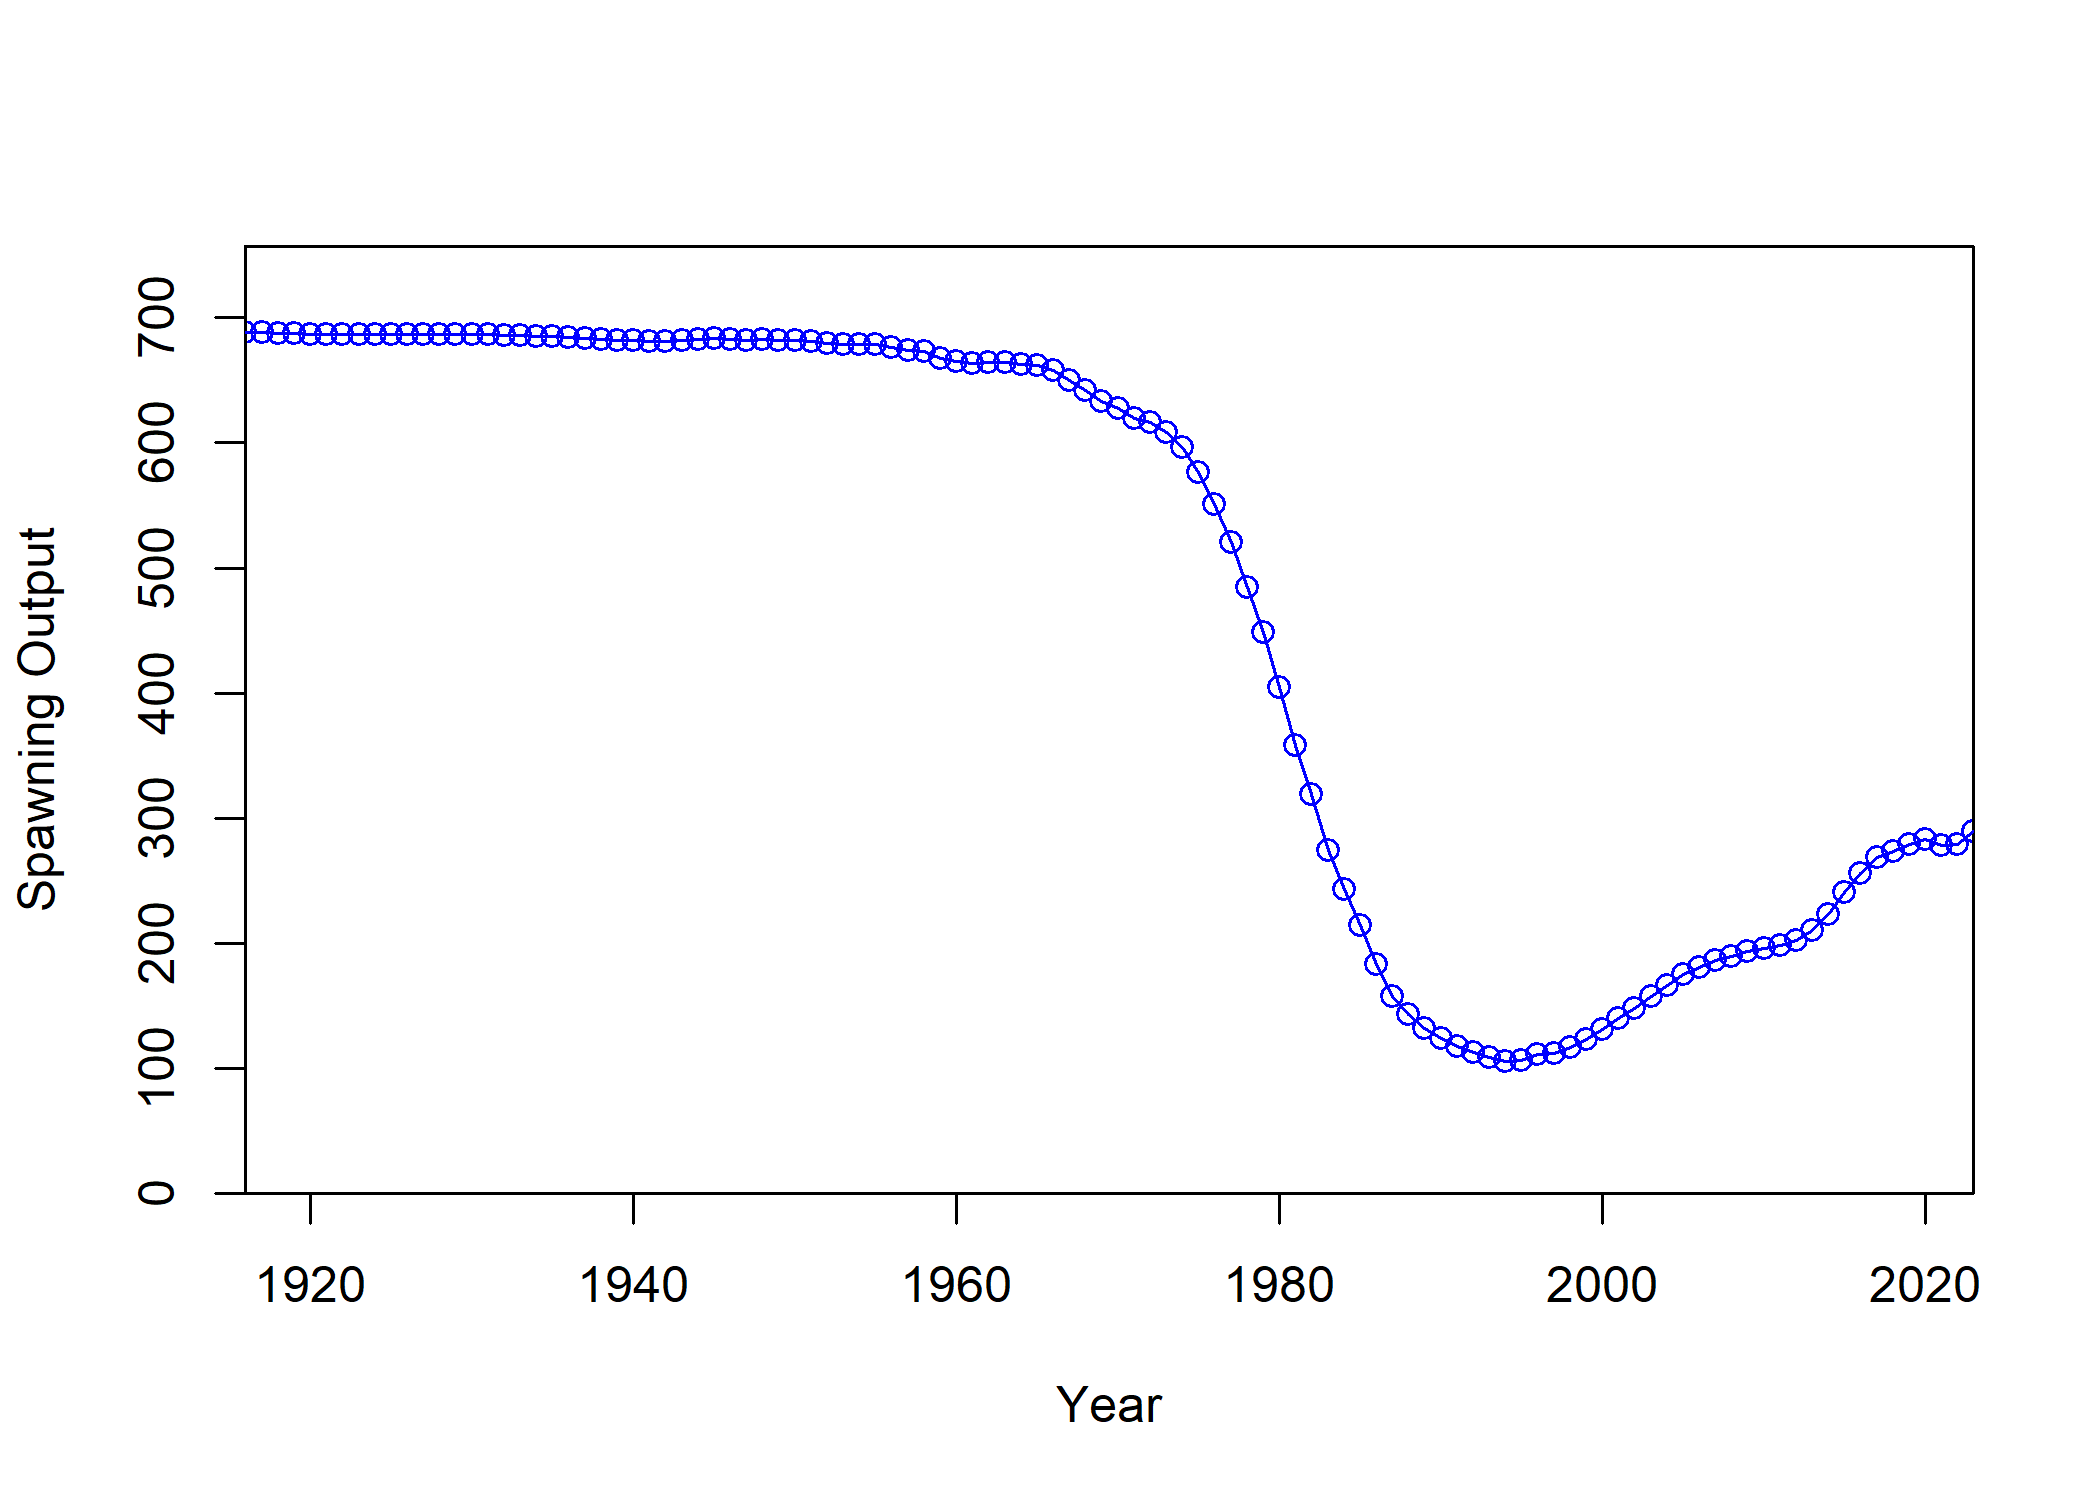
\includegraphics[alt=See Table 23.,width=1\textwidth,height=1\textheight]{C:/Users/melissa.monk/Documents/GitHub/copper_rockfish_2023/documents/shared_figures/spawning_output_combined.png}
}
\caption{Estimated combined time series of spawning output for copper rockfish in California waters.\label{fig:es-sb-all}}
\end{figure}

\begin{figure}
{\centering
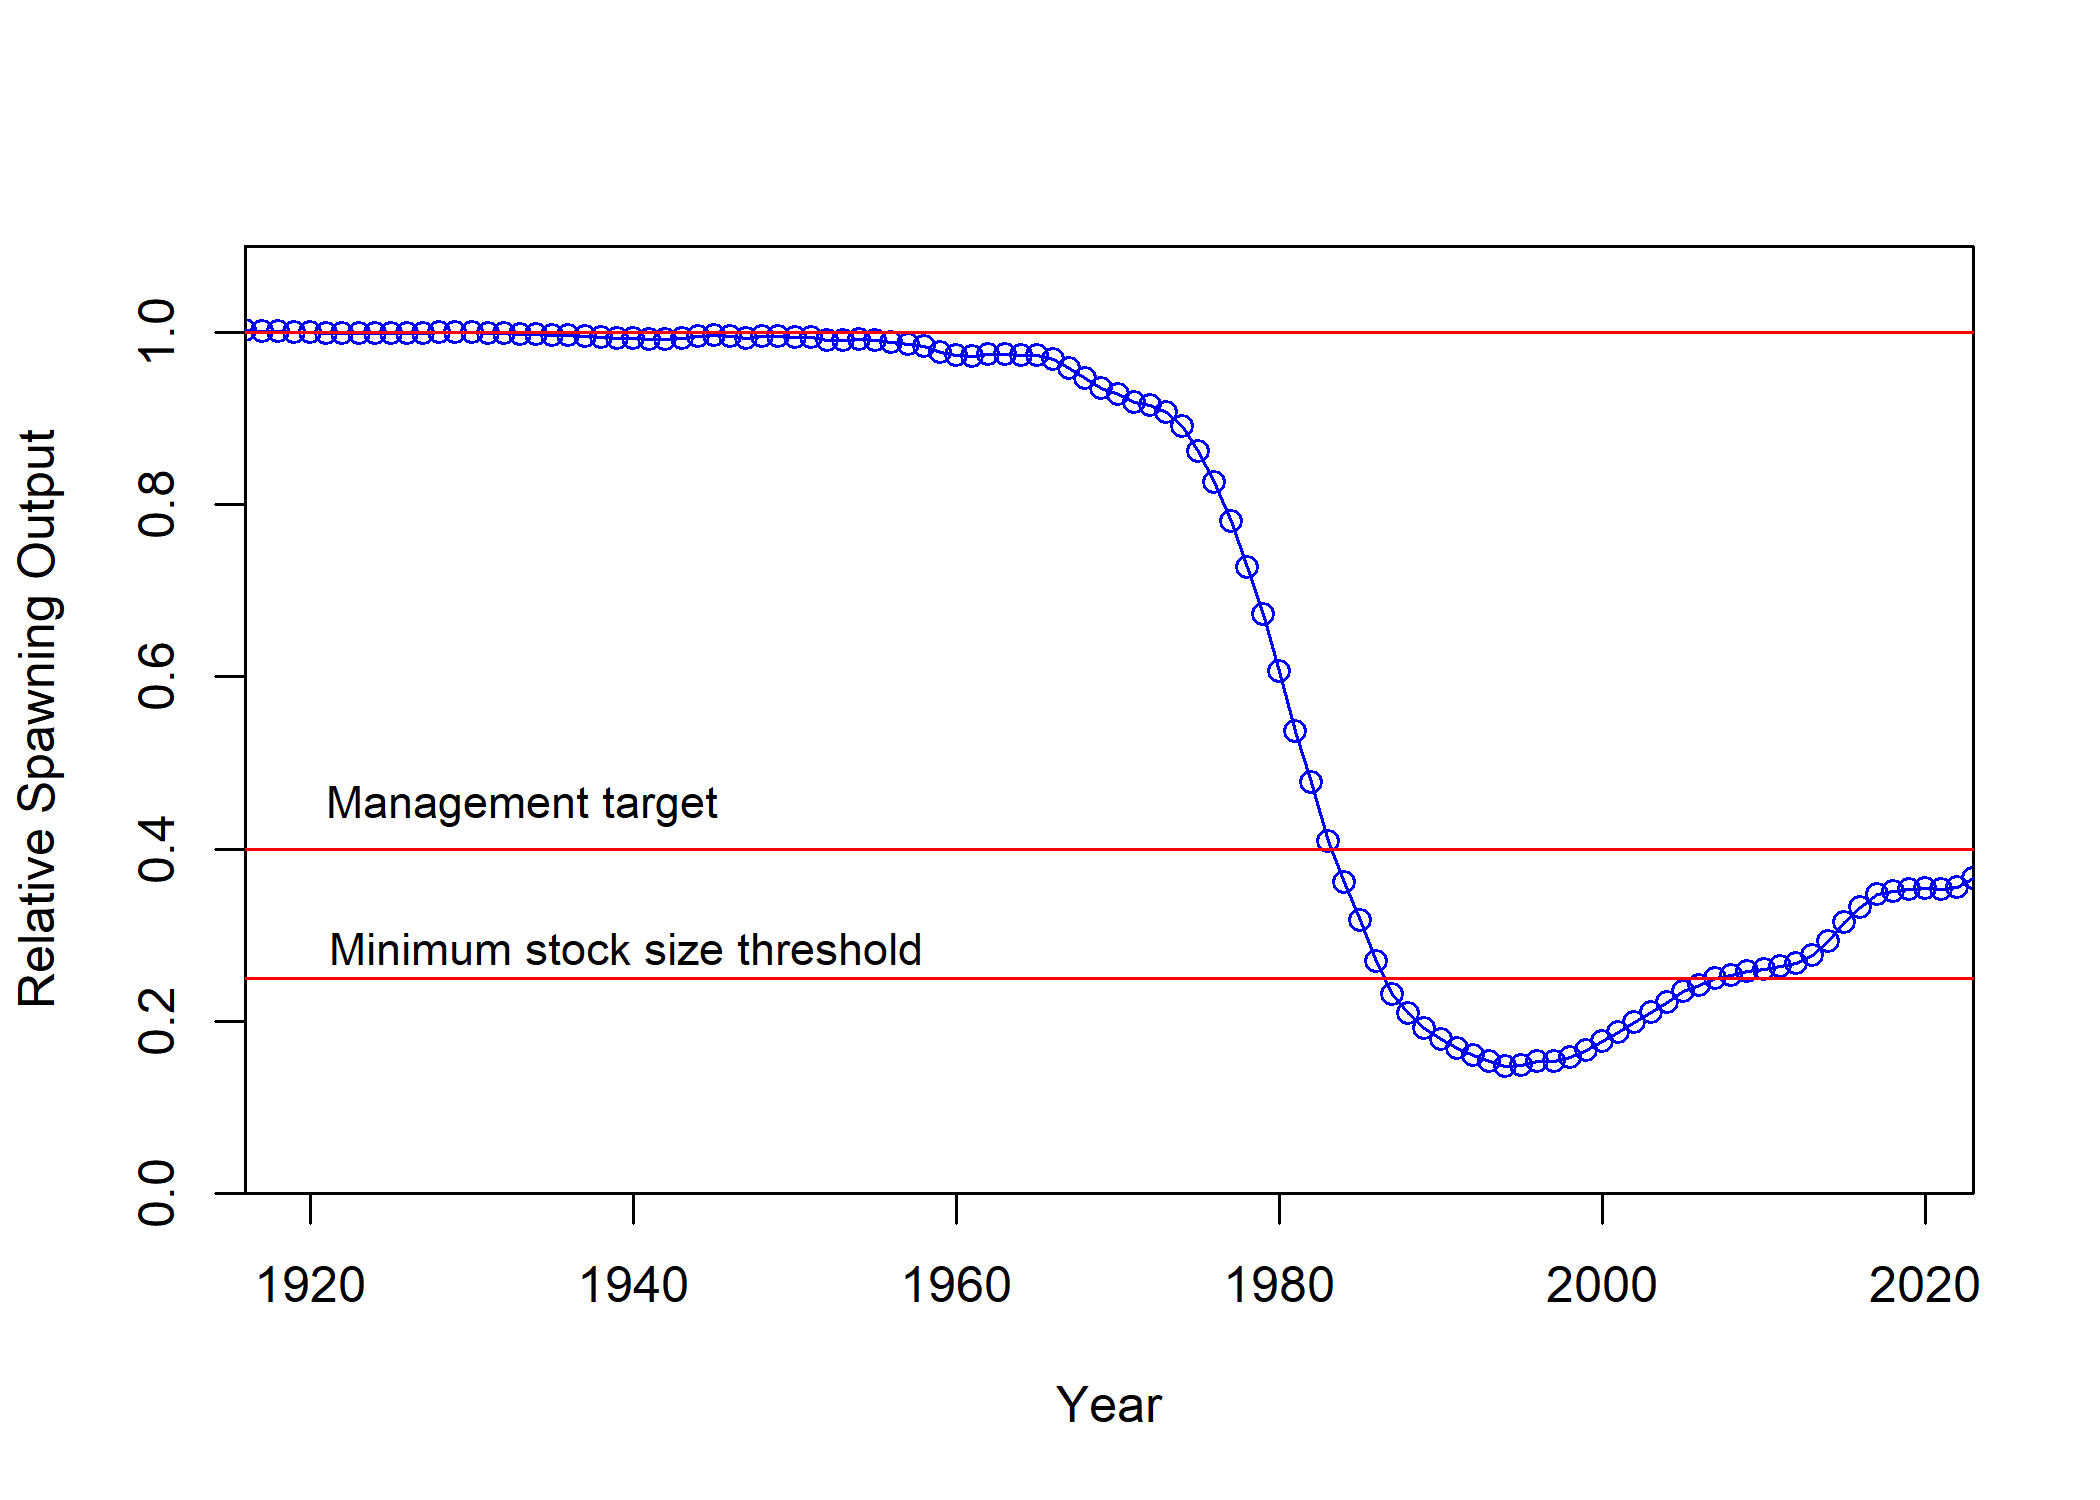
\includegraphics[alt=See Table 23.,width=1\textwidth,height=1\textheight]{C:/Users/melissa.monk/Documents/GitHub/copper_rockfish_2023/documents/shared_figures/depletion_combined.png}
}
\caption{Estimated combined time series of fraction of relative spawning output for copper rockfish in California waters.\label{fig:es-depl-all}}
\end{figure}

\begin{figure}
{\centering
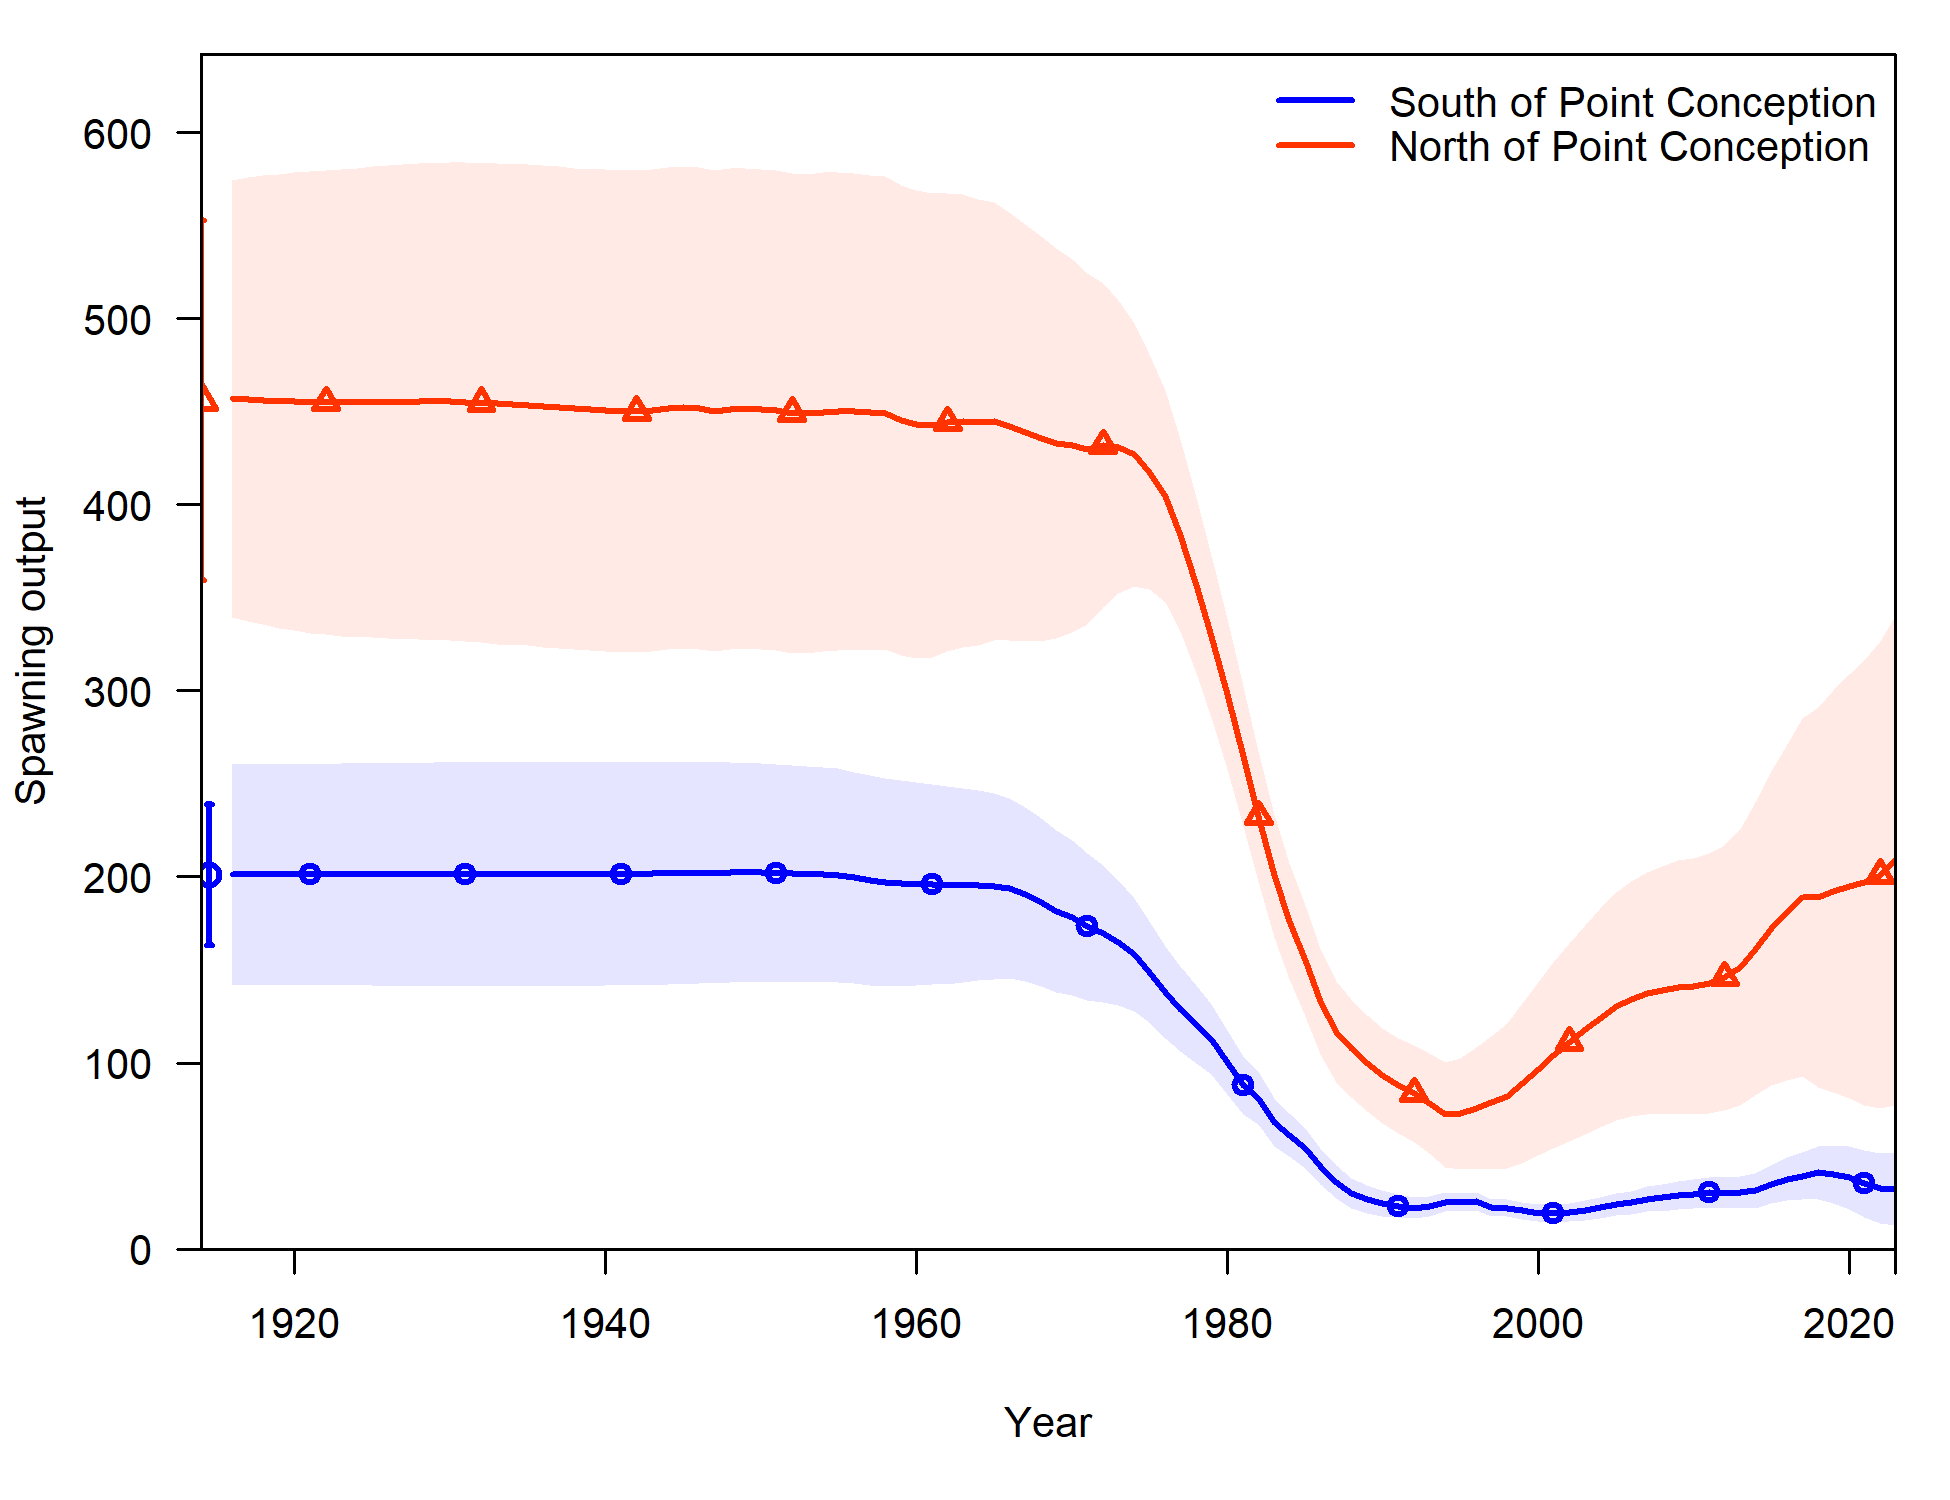
\includegraphics[alt=See Table 22 in this document and Table 15 in the north of Point Conception assessment document.,width=1\textwidth,height=1\textheight]{C:/Users/melissa.monk/Documents/GitHub/copper_rockfish_2023/documents/shared_figures/compare2_spawnbio_uncertainty.png}
}
\caption{Estimated time series of spawning output (circles and line: median; light broken lines: 95 percent intervals) for the model areas south and north of Point Conception.\label{fig:es-sb}}
\end{figure}

\begin{figure}
{\centering
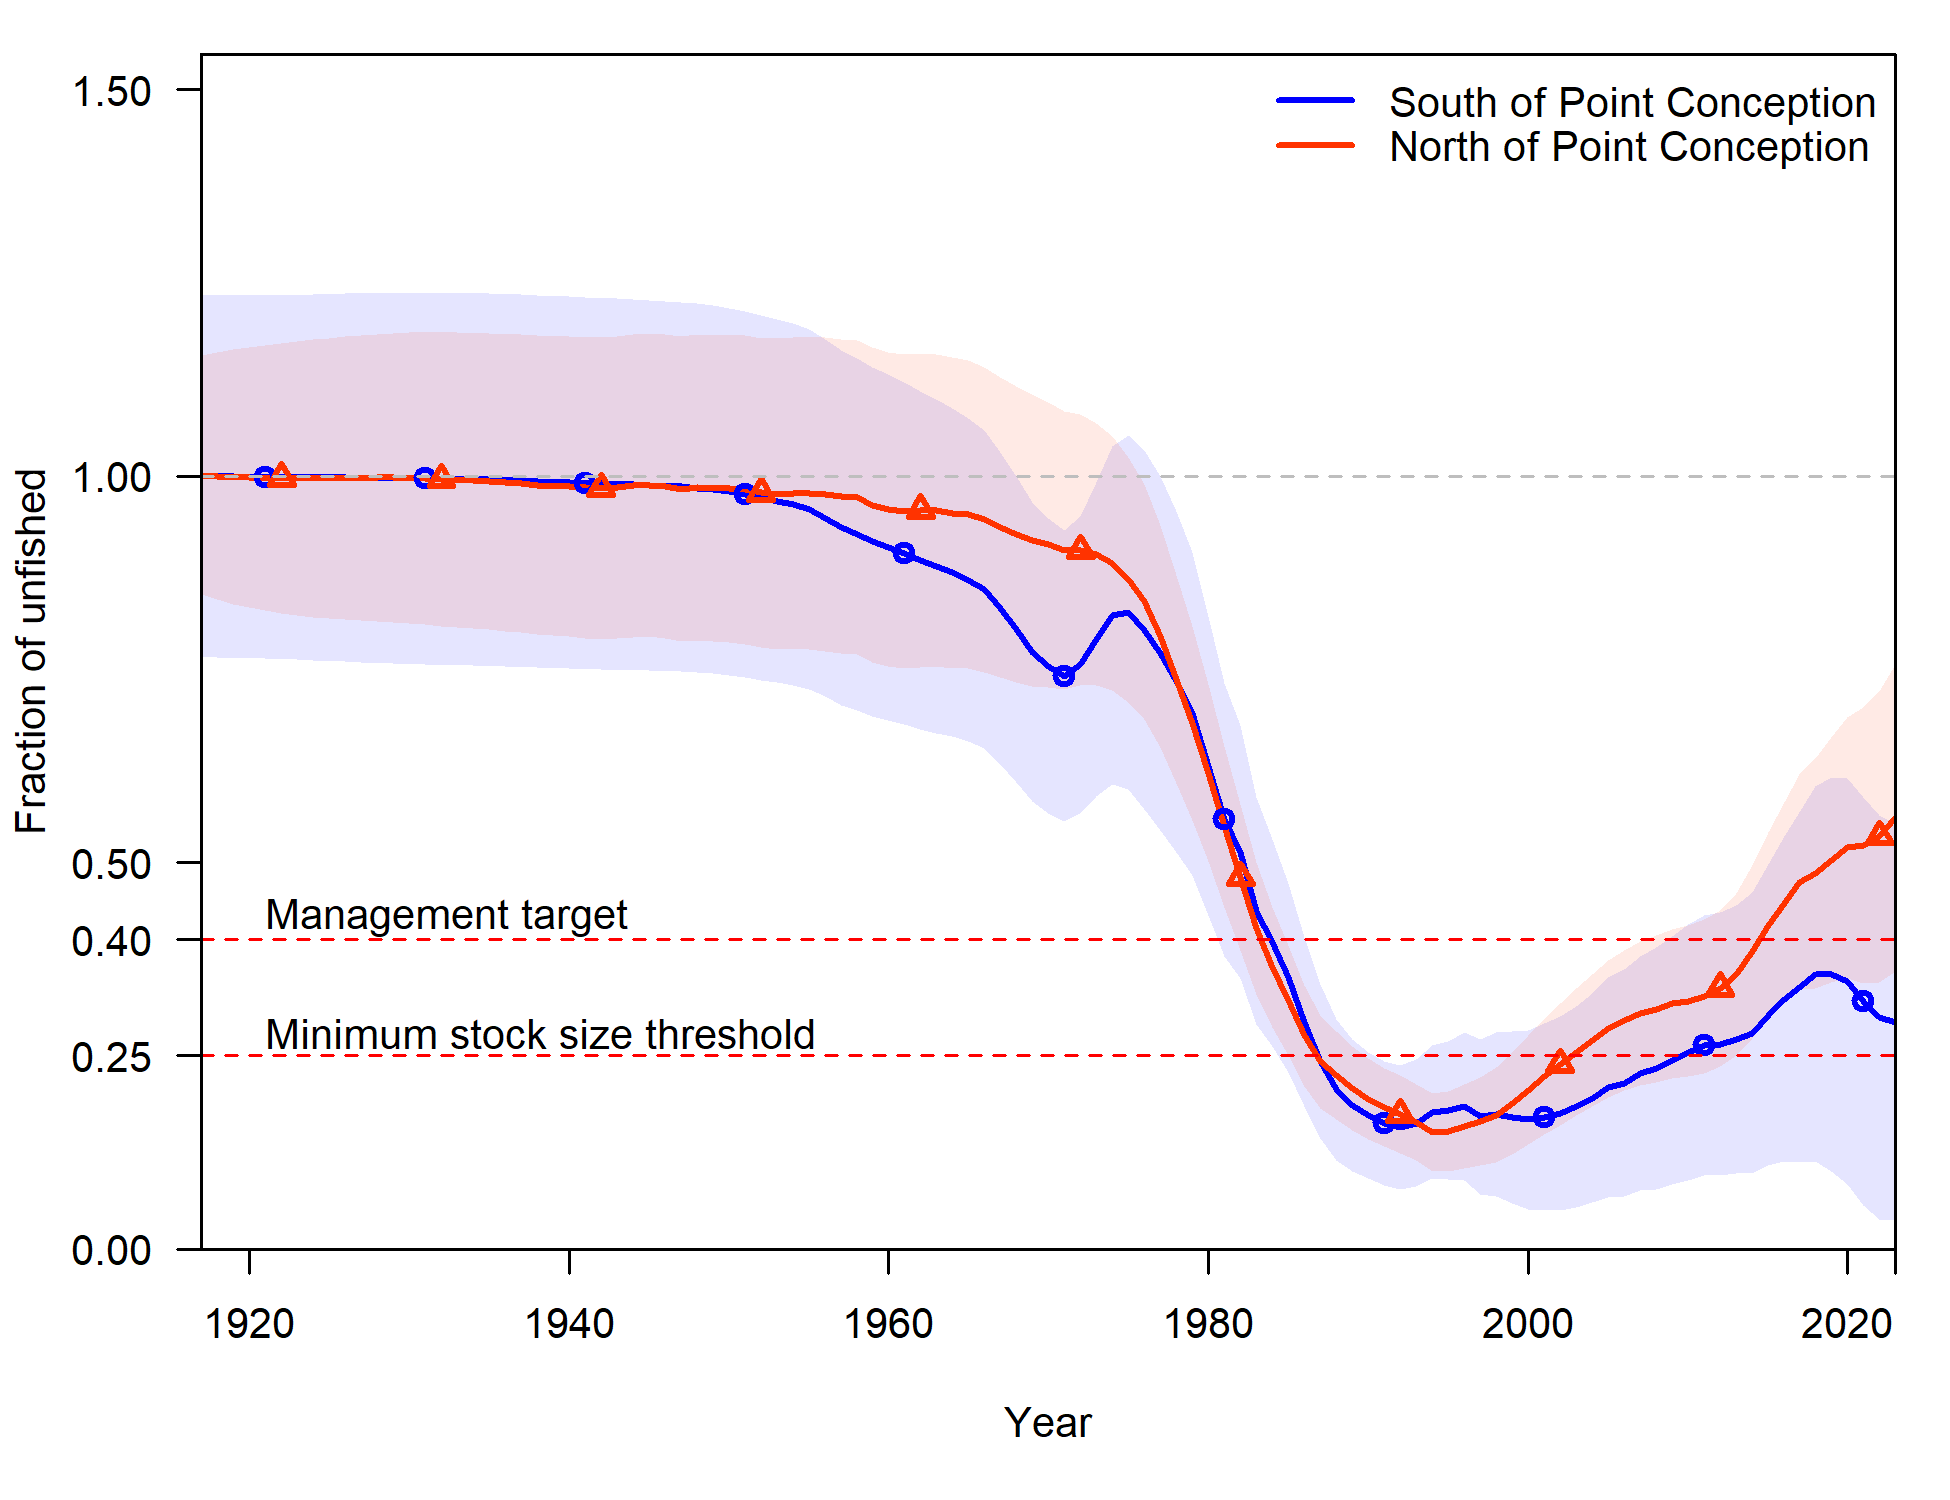
\includegraphics[alt=See Table 22 in this document and Table 15 in the north of Point Conception assessment document.,width=1\textwidth,height=1\textheight]{C:/Users/melissa.monk/Documents/GitHub/copper_rockfish_2023/documents/shared_figures/compare4_Bratio_uncertainty.png}
}
\caption{Estimated time series of fraction of relative spawning output (circles and line: median; light broken lines: 95 percent intervals) for the model areas south and north of Point Conception.\label{fig:es-depl}}
\end{figure}

\pagebreak

\subsection*{Recruitment}\label{recruitment}
\addcontentsline{toc}{subsection}{Recruitment}

Recruitment deviations were estimated from 1965-2020 south of Point Conception and from 1970-2019 north of Point Conception. The estimated magnitude of recruitment deviations and years of strong or weak recruitment varied for each sub-area. The base model south of Point Conception estimated strong recruitment in 2009, 2010, and 2013 with multiple poor recruitment years at the end of the time series (Table \ref{tab:south-recrES} and Figures \ref{fig:es-recruits} and \ref{fig:es-rec-devs}). The sub-area model north of Point Conception estimated the largest recent recruitment deviations in 2007, 2009, and 2017 with series of poor recruitment occurring in the late 1990s and early 2000s (Table \ref{tab:north-recrES} and Figures \ref{fig:es-recruits} and \ref{fig:es-rec-devs}). The magnitude of overall estimated relative recruitment variation, highs and lows, was greater in the sub-area south of Point Conception compared to the sub-area north of Point Conception.

\begingroup\fontsize{10}{12}\selectfont
\begingroup\fontsize{10}{12}\selectfont

\begin{longtable}[t]{r>{\centering\arraybackslash}p{1.57cm}>{\centering\arraybackslash}p{1.57cm}>{\centering\arraybackslash}p{1.57cm}>{\centering\arraybackslash}p{1.57cm}>{\centering\arraybackslash}p{1.57cm}>{\centering\arraybackslash}p{1.57cm}}
\caption{\label{tab:south-recrES}Estimated recent trend in recruitment and recruitment deviations and the 95 percent intervals for the sub-area model south of Point Conception.}\\
\toprule
Year & Recruitment & Lower Interval & Upper Interval & Recruitment Deviations & Lower Interval & Upper Interval\\
\midrule
\endfirsthead
\caption[]{Estimated recent trend in recruitment and recruitment deviations and the 95 percent intervals for the sub-area model south of Point Conception. \textit{(continued)}}\\
\toprule
Year & Recruitment & Lower Interval & Upper Interval & Recruitment Deviations & Lower Interval & Upper Interval\\
\midrule
\endhead

\endfoot
\bottomrule
\endlastfoot
2013 & 613.62 & 381.00 & 988.26 & 1.18 & 0.94 & 1.41\\
2014 & 168.22 & 86.76 & 326.18 & -0.13 & -0.64 & 0.39\\
2015 & 81.26 & 39.81 & 165.88 & -0.88 & -1.45 & -0.30\\
2016 & 114.55 & 59.49 & 220.57 & -0.55 & -1.00 & -0.09\\
2017 & 91.14 & 44.28 & 187.61 & -0.79 & -1.33 & -0.25\\
2018 & 91.39 & 42.11 & 198.33 & -0.80 & -1.40 & -0.19\\
2019 & 119.56 & 51.10 & 279.76 & -0.53 & -1.24 & 0.18\\
2020 & 119.75 & 43.77 & 327.64 & -0.60 & -1.54 & 0.34\\
2021 & 231.44 & 144.36 & 371.04 & 0.00 & 0.00 & 0.00\\
2022 & 227.42 & 138.88 & 372.42 & 0.00 & 0.00 & 0.00\\
2023 & 226.18 & 137.68 & 371.57 & 0.00 & 0.00 & 0.00\\*
\end{longtable}
\endgroup{}
\endgroup{}


\newpage

\begingroup\fontsize{10}{12}\selectfont
\begingroup\fontsize{10}{12}\selectfont

\begin{longtable}[t]{r>{\centering\arraybackslash}p{1.57cm}>{\centering\arraybackslash}p{1.57cm}>{\centering\arraybackslash}p{1.57cm}>{\centering\arraybackslash}p{1.57cm}>{\centering\arraybackslash}p{1.57cm}>{\centering\arraybackslash}p{1.57cm}}
\caption{\label{tab:north-recrES}Estimated recent trend in recruitment and recruitment deviations and the 95 percent intervals for the sub-area model north of Point Conception.}\\
\toprule
Year & Recruitment & Lower Interval & Upper Interval & Recruitment Deviations & Lower Interval & Upper Interval\\
\midrule
\endfirsthead
\caption[]{Estimated recent trend in recruitment and recruitment deviations and the 95 percent intervals for the sub-area model north of Point Conception. \textit{(continued)}}\\
\toprule
Year & Recruitment & Lower Interval & Upper Interval & Recruitment Deviations & Lower Interval & Upper Interval\\
\midrule
\endhead

\endfoot
\bottomrule
\endlastfoot
2013 & 556.60 & 282.67 & 1095.99 & 0.23 & -0.38 & 0.84\\
2014 & 466.50 & 233.22 & 933.12 & 0.04 & -0.59 & 0.67\\
2015 & 590.78 & 316.19 & 1103.84 & 0.26 & -0.27 & 0.79\\
2016 & 285.96 & 134.46 & 608.15 & -0.47 & -1.18 & 0.24\\
2017 & 869.76 & 474.53 & 1594.18 & 0.63 & 0.13 & 1.12\\
2018 & 618.32 & 318.82 & 1199.18 & 0.25 & -0.34 & 0.84\\
2019 & 345.34 & 159.74 & 746.57 & -0.37 & -1.11 & 0.37\\
2020 & 502.19 & 394.01 & 640.08 & 0.00 & 0.00 & 0.00\\
2021 & 503.74 & 394.44 & 643.32 & 0.00 & 0.00 & 0.00\\
2022 & 505.86 & 395.70 & 646.68 & 0.00 & 0.00 & 0.00\\
2023 & 509.39 & 398.85 & 650.56 & 0.00 & 0.00 & 0.00\\*
\end{longtable}
\endgroup{}
\endgroup{}


\begin{figure}
{\centering
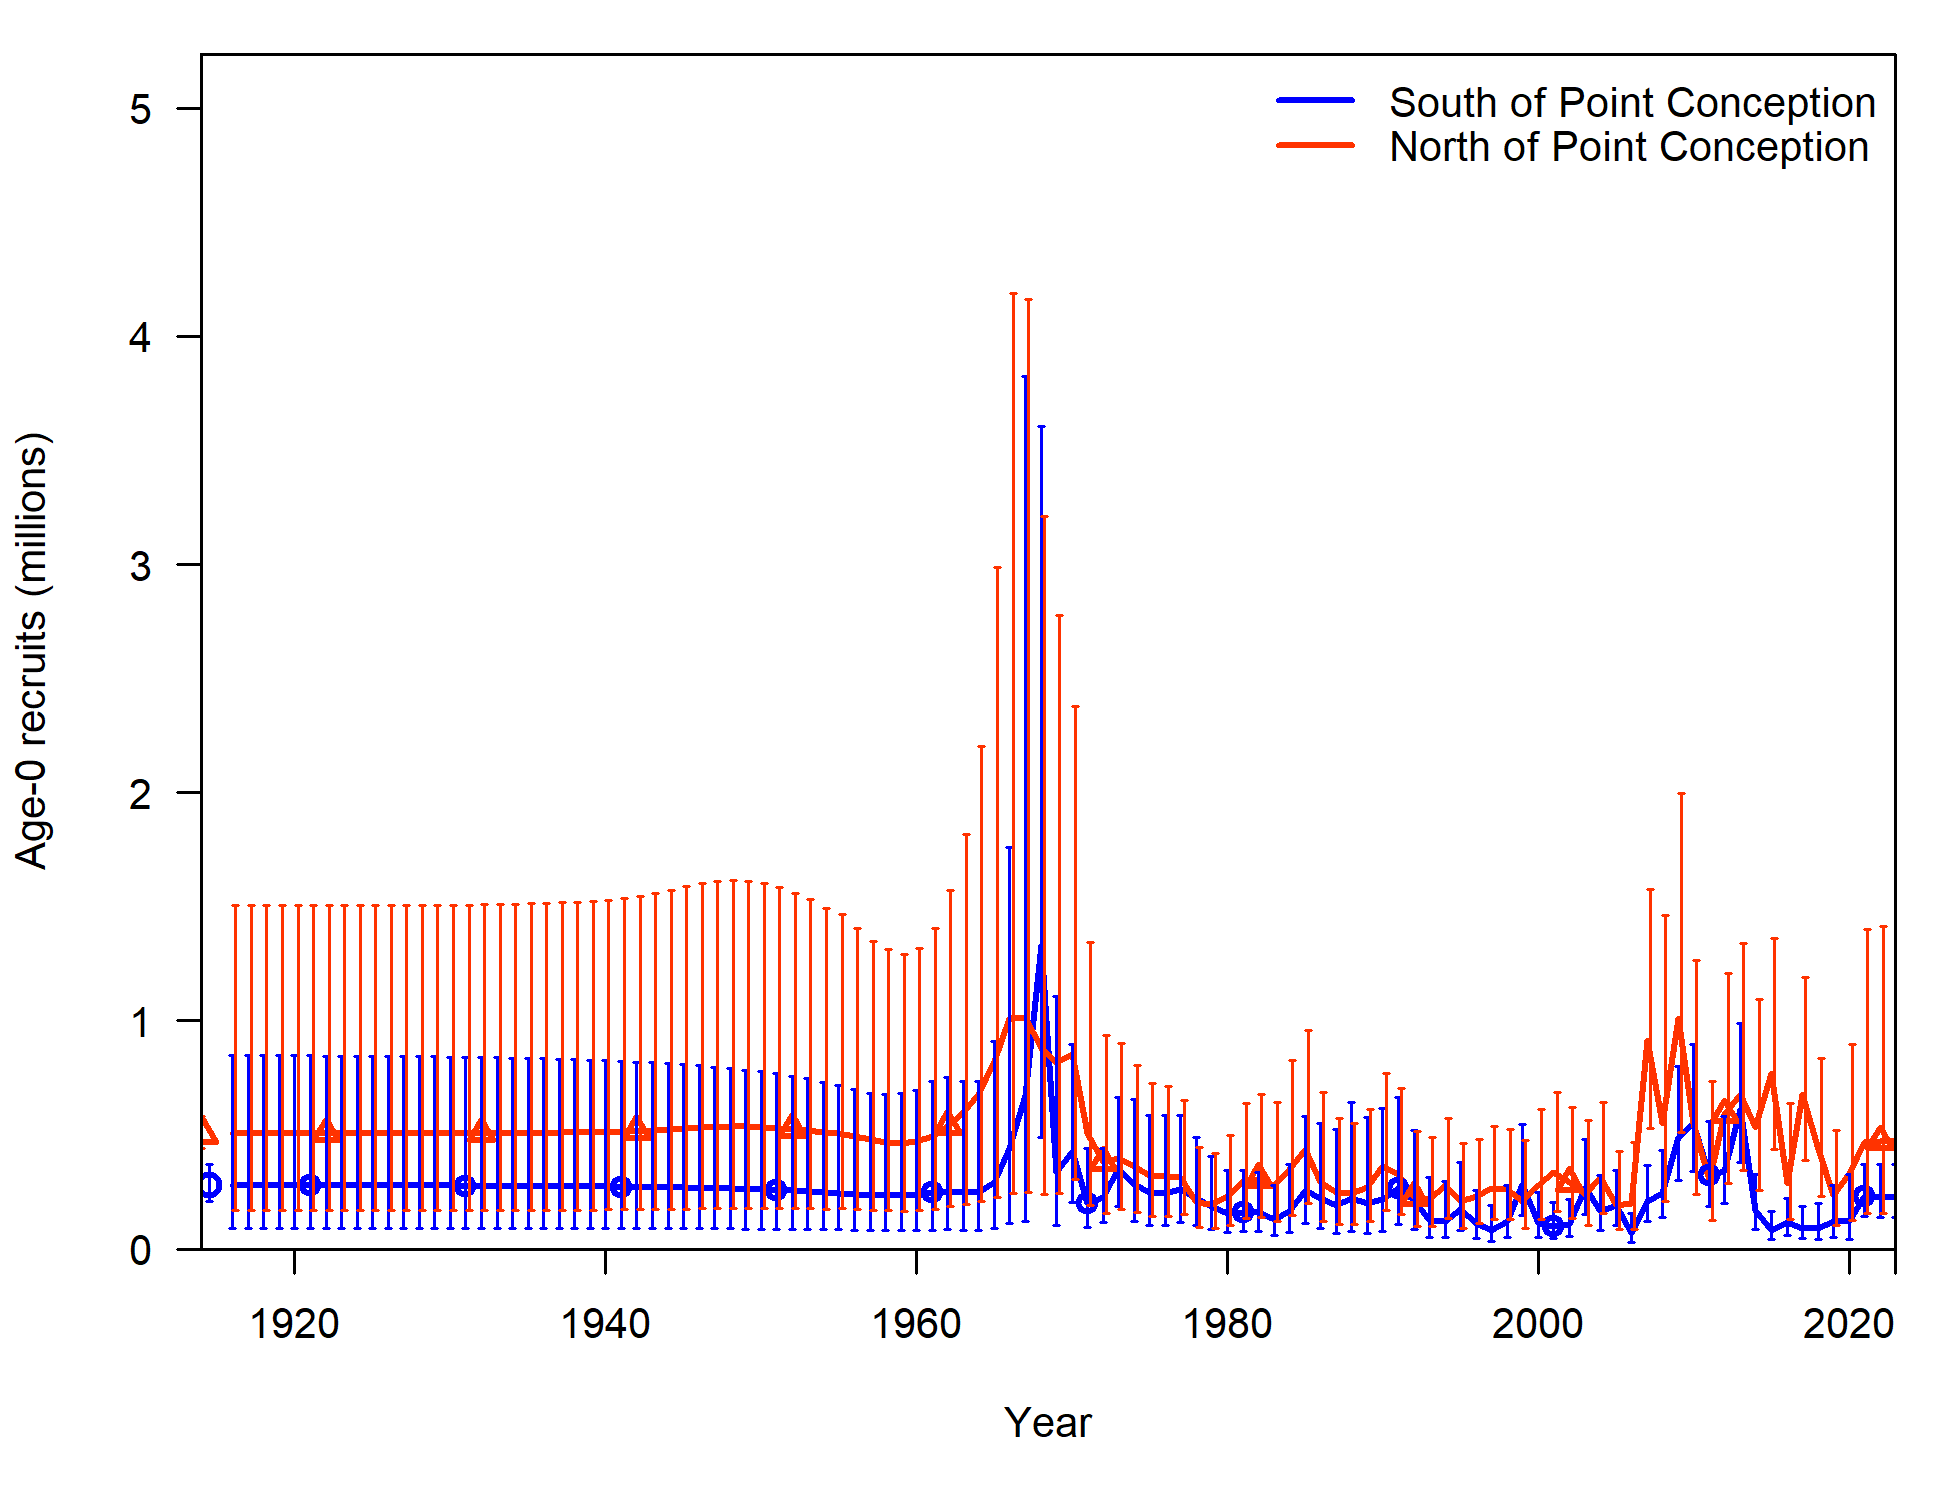
\includegraphics[alt=See Table 22 in this document and Table 15 in the north of Point Conception assessment document.,width=1\textwidth,height=1\textheight]{C:/Users/melissa.monk/Documents/GitHub/copper_rockfish_2023/documents/shared_figures/compare10_recruits_uncertainty.png}
}
\caption{Estimated time series of age-0 recruits (1000s) for the model areas south and north of Point Conception with 95 percent intervals.\label{fig:es-recruits}}
\end{figure}

\begin{figure}
{\centering
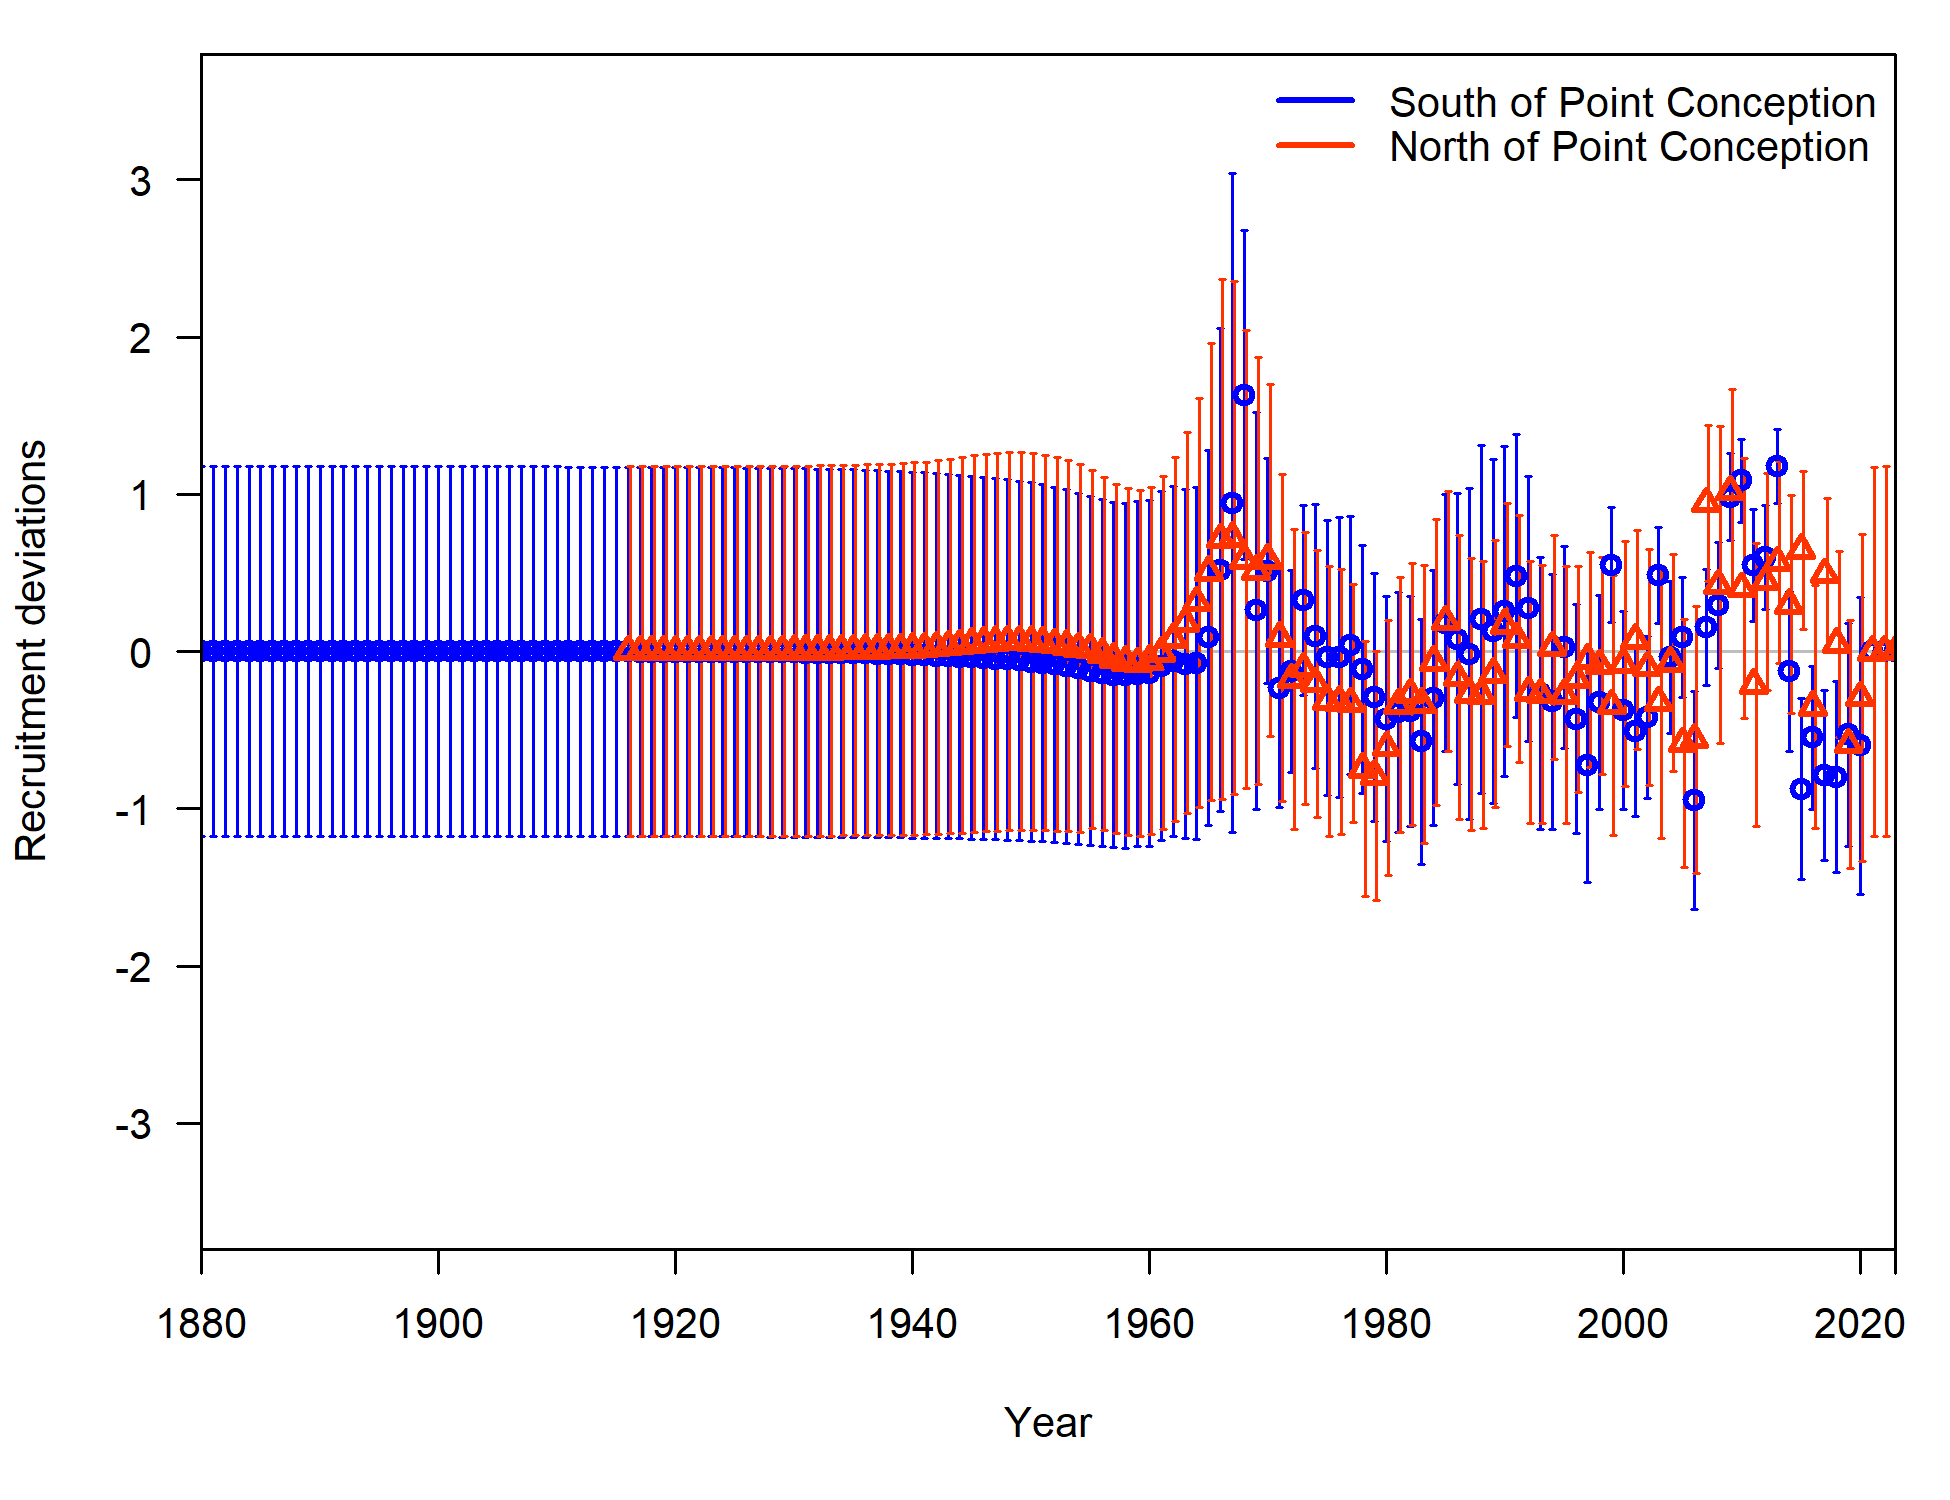
\includegraphics[alt=See Table vi and vii.,width=1\textwidth,height=1\textheight]{C:/Users/melissa.monk/Documents/GitHub/copper_rockfish_2023/documents/shared_figures/compare12_recdevs_uncertainty.png}
}
\caption{Estimated time series of recruitment deviations for the model areas south and north of Point Conception.\label{fig:es-rec-devs}}
\end{figure}

\clearpage

\subsection*{Exploitation status}\label{exploitation-status}
\addcontentsline{toc}{subsection}{Exploitation status}

Trends in fishing intensity (1 - SPR) for both sub-areas dramatically increased in the 1970s, exceeded the management target \(\text{SPR}_{50\%}\), and remained high until at least the late 1990s (Figure \ref{fig:es-1-spr}). The fishing intensity south of Point Conception declined in the early 2000s but remained above the target for the rest of the time series except for 2006 (Table \ref{tab:south-exploitES}). The fishing intensity sharply decreased around 2000 north of Point Conception with fishing intensity remaining below the management target since, excluding a recent spike in 2017 (Table \ref{tab:north-exploitES}).

As a percentage of biomass (ages 3+), harvest rates south of Point Conception between 2013-2021 ranged between 0.13-0.19, with harvest rates declining in 2022 to 0.06 based on inseason management actions by California Department of Fish and Wildlife (CDFW) that reduced the sub-bag limit for copper rockfish to one fish across the state (Table \ref{tab:south-exploitES}). The harvest rates in the sub-area north of Point Conception since 2013 have ranged between 0.01-0.07 (Table \ref{tab:north-exploitES}).

\begingroup\fontsize{10}{12}\selectfont
\begingroup\fontsize{10}{12}\selectfont

\begin{longtable}[t]{r>{\centering\arraybackslash}p{1.57cm}>{\centering\arraybackslash}p{1.57cm}>{\centering\arraybackslash}p{1.57cm}>{\centering\arraybackslash}p{1.57cm}>{\centering\arraybackslash}p{1.57cm}>{\centering\arraybackslash}p{1.57cm}}
\caption{\label{tab:south-exploitES}Estimated recent trend in the 1-SPR where SPR is the spawning potential ratio the exploitation rate, and the 95 percent intervals for the sub-area model south of Point Conception.}\\
\toprule
Year & 1-SPR & Lower Interval & Upper Interval & Exploitation Rate & Lower Interval & Upper Interval\\
\midrule
\endfirsthead
\caption[]{Estimated recent trend in the 1-SPR where SPR is the spawning potential ratio the exploitation rate, and the 95 percent intervals for the sub-area model south of Point Conception. \textit{(continued)}}\\
\toprule
Year & 1-SPR & Lower Interval & Upper Interval & Exploitation Rate & Lower Interval & Upper Interval\\
\midrule
\endhead

\endfoot
\bottomrule
\endlastfoot
2013 & 0.71 & 0.52 & 0.90 & 0.11 & 0.05 & 0.17\\
2014 & 0.59 & 0.39 & 0.79 & 0.08 & 0.04 & 0.13\\
2015 & 0.66 & 0.46 & 0.86 & 0.10 & 0.05 & 0.16\\
2016 & 0.71 & 0.51 & 0.90 & 0.12 & 0.05 & 0.18\\
2017 & 0.67 & 0.46 & 0.88 & 0.10 & 0.04 & 0.16\\
2018 & 0.75 & 0.55 & 0.95 & 0.12 & 0.05 & 0.20\\
2019 & 0.72 & 0.50 & 0.94 & 0.11 & 0.03 & 0.18\\
2020 & 0.80 & 0.59 & 1.01 & 0.12 & 0.03 & 0.21\\
2021 & 0.72 & 0.47 & 0.98 & 0.09 & 0.02 & 0.17\\
2022 & 0.40 & 0.15 & 0.64 & 0.03 & 0.01 & 0.06\\*
\end{longtable}
\endgroup{}
\endgroup{}


\newpage

\begingroup\fontsize{10}{12}\selectfont
\begingroup\fontsize{10}{12}\selectfont

\begin{longtable}[t]{r>{\centering\arraybackslash}p{1.57cm}>{\centering\arraybackslash}p{1.57cm}>{\centering\arraybackslash}p{1.57cm}>{\centering\arraybackslash}p{1.57cm}>{\centering\arraybackslash}p{1.57cm}>{\centering\arraybackslash}p{1.57cm}}
\caption{\label{tab:north-exploitES}Estimated recent trend in the 1-SPR where SPR is the spawning potential ratio the exploitation rate, and the 95 percent intervals for the sub-area model north of Point Conception.}\\
\toprule
Year & 1-SPR & Lower Interval & Upper Interval & Exploitation Rate & Lower Interval & Upper Interval\\
\midrule
\endfirsthead
\caption[]{Estimated recent trend in the 1-SPR where SPR is the spawning potential ratio the exploitation rate, and the 95 percent intervals for the sub-area model north of Point Conception. \textit{(continued)}}\\
\toprule
Year & 1-SPR & Lower Interval & Upper Interval & Exploitation Rate & Lower Interval & Upper Interval\\
\midrule
\endhead

\endfoot
\bottomrule
\endlastfoot
2013 & 0.16 & 0.10 & 0.22 & 0.01 & 0.01 & 0.02\\
2014 & 0.20 & 0.13 & 0.27 & 0.02 & 0.01 & 0.02\\
2015 & 0.31 & 0.21 & 0.41 & 0.03 & 0.02 & 0.04\\
2016 & 0.31 & 0.20 & 0.41 & 0.03 & 0.02 & 0.04\\
2017 & 0.50 & 0.37 & 0.63 & 0.05 & 0.03 & 0.08\\
2018 & 0.41 & 0.28 & 0.53 & 0.04 & 0.02 & 0.06\\
2019 & 0.40 & 0.27 & 0.53 & 0.04 & 0.02 & 0.06\\
2020 & 0.53 & 0.38 & 0.67 & 0.06 & 0.03 & 0.08\\
2021 & 0.41 & 0.27 & 0.55 & 0.04 & 0.02 & 0.06\\
2022 & 0.21 & 0.12 & 0.30 & 0.02 & 0.01 & 0.03\\*
\end{longtable}
\endgroup{}
\endgroup{}


\begin{figure}
{\centering
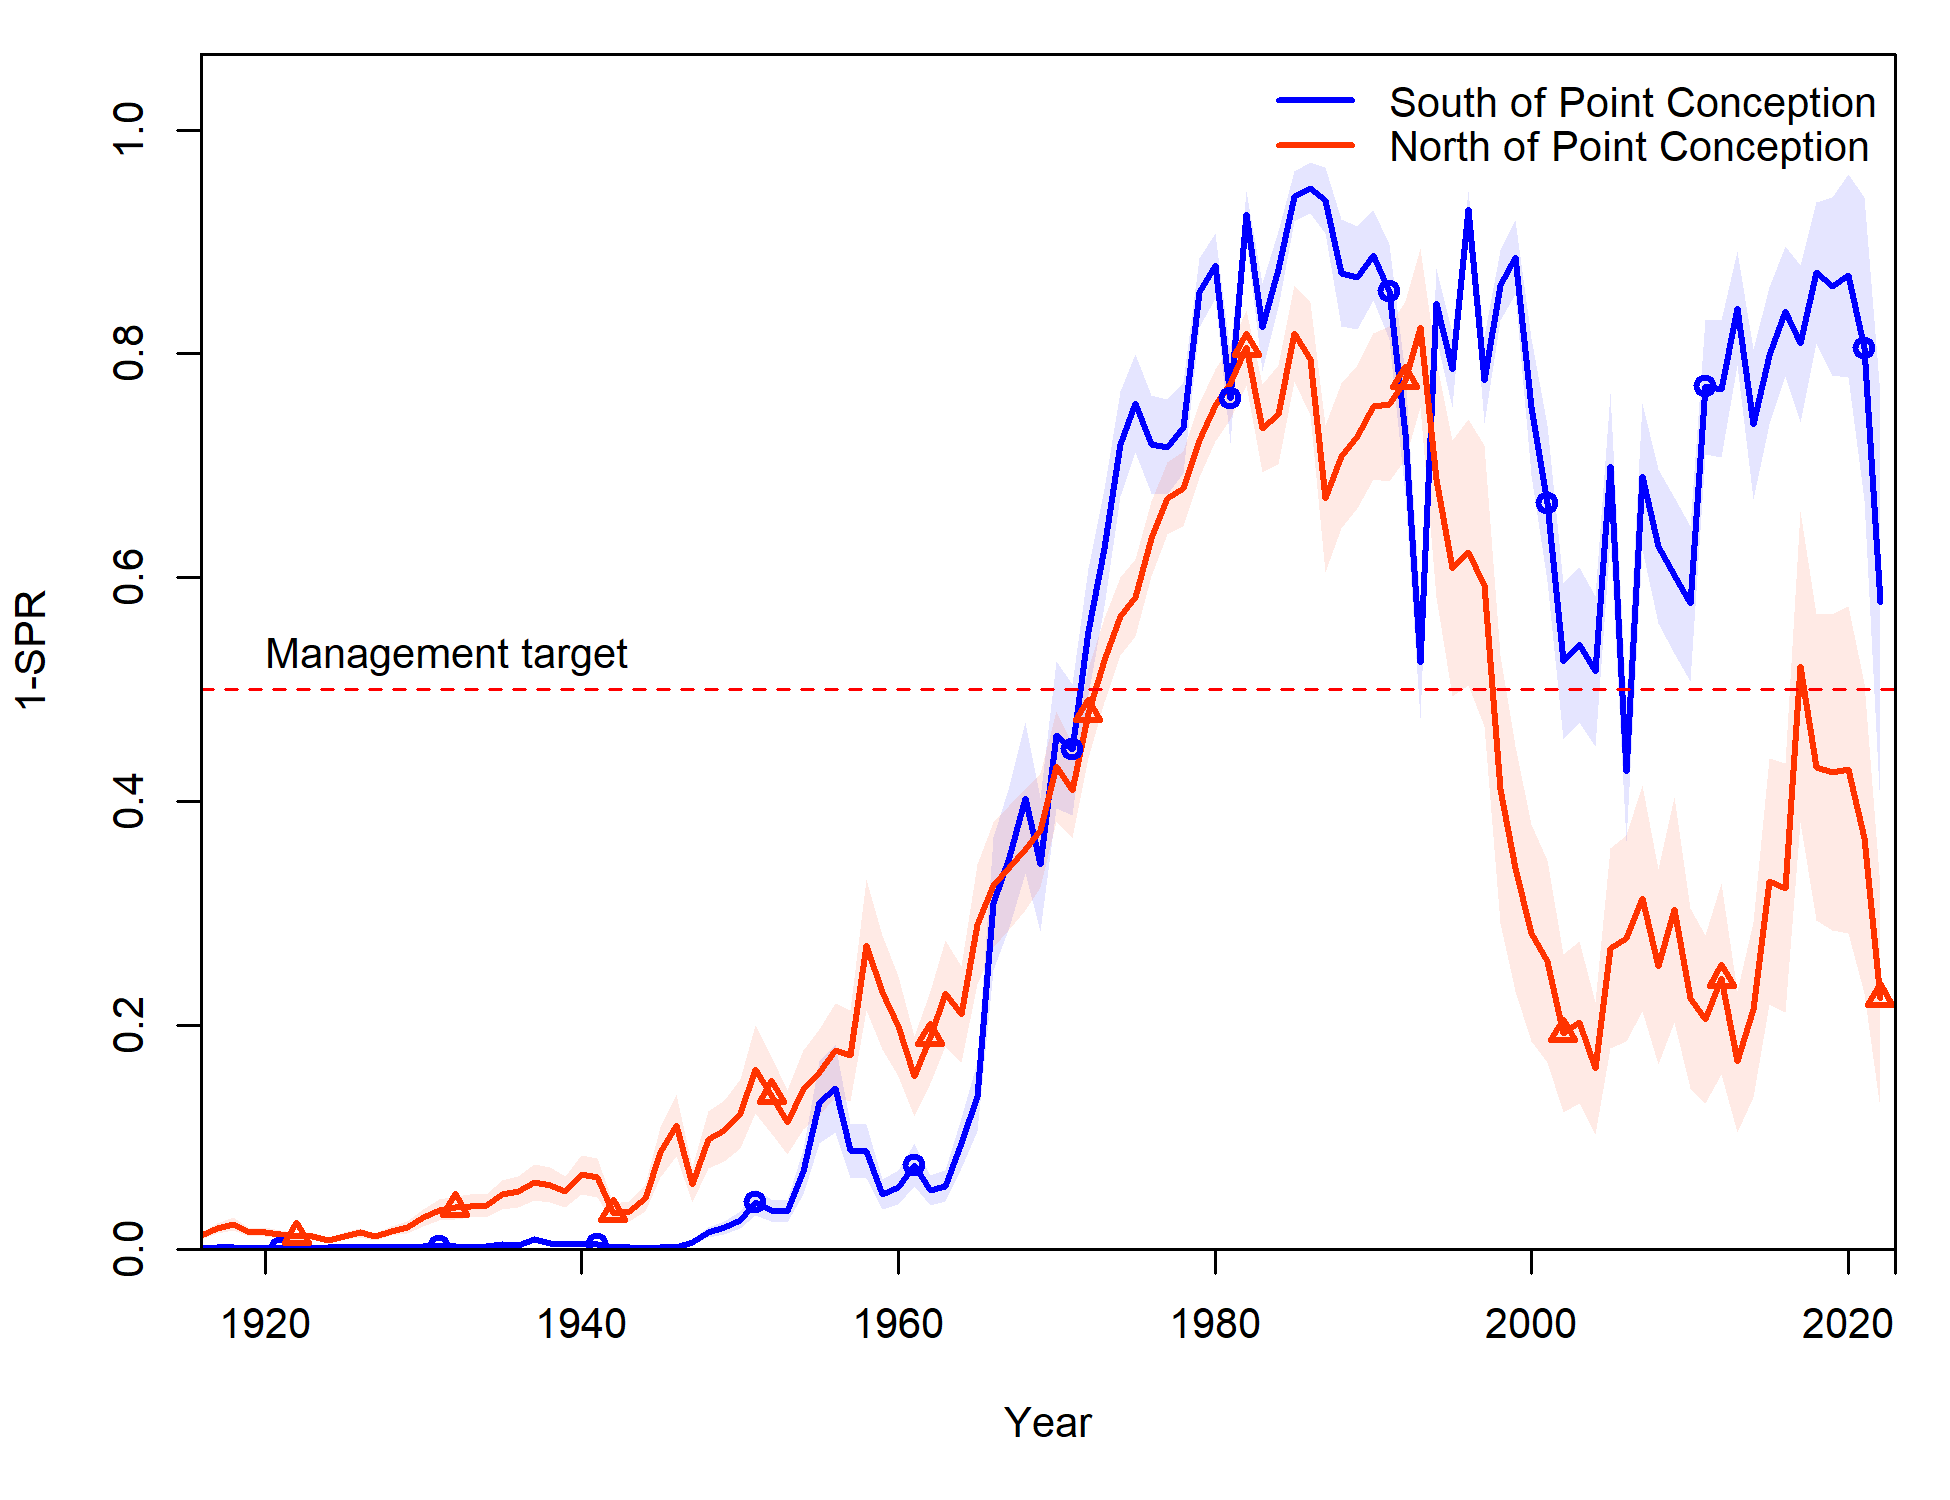
\includegraphics[alt=See Table 22 in this document and Table 15 in the north of Point Conception assessment document.,width=1\textwidth,height=1\textheight]{C:/Users/melissa.monk/Documents/GitHub/copper_rockfish_2023/documents/shared_figures/compare6_SPRratio_uncertainty.png}
}
\caption{Estimated 1 - relative spawning ratio (SPR) by year for the model areas south and north of Point Conception. The management target is plotted as a red horizontal line and values above this reflect harvest in excess of the proxy harvest rate.\label{fig:es-1-spr}}
\end{figure}

\pagebreak

\subsection*{Ecosystem considerations}\label{ecosystem-considerations}
\addcontentsline{toc}{subsection}{Ecosystem considerations}

This stock assessment does not explicitly incorporate trophic interactions, habitat factors (other than as they inform relative abundance indices) or environmental factors into the assessment model, but a brief description of likely or potential ecosystem considerations is provided below.

As with most other rockfish and groundfish in the California Current, recruitment or cohort (year-class) strength appears to be highly variable for copper rockfish, with only a modest apparent relationship to estimated levels of spawning output. Oceanographic and ecosystem factors are widely recognized to be key drivers of recruitment variability for most species of groundfish, as well as most elements of California Current food webs. Empirical estimates of recruitment from pelagic juvenile rockfish surveys have been used to inform incoming year class strength for some of these stocks, however copper rockfish are infrequently encountered in these surveys. Between 1998 and 2013 the California Cooperative Oceanic Fisheries Investigation (CalCOFI) survey had 34 positive observations of copper rockfish out of over 500 bongo net tows.

\subsection*{Reference points}\label{reference-points}
\addcontentsline{toc}{subsection}{Reference points}

Reference points were calculated using the estimated selectivities and catch distribution among fleets in the final year of each sub-area model, 2022. Reference points are presented in Tables \ref{tab:south-referenceES} and \ref{tab:north-referenceES} for each sub-model area and are informational only. Copper rockfish off the California coast are managed as a single stock by the Pacific Fishery Management Council. Combined reference point quantities for the California stock are shown in Table \ref{tab:ref-point-all-es}.

Sustainable total yield (landings plus discards) across California is estimated to 164.24 mt when using an \(\text{SPR}_{50\%}\) reference harvest rate. The spawning output equivalent to 40 percent of the unfished level (\(\text{SO}_{40\%}\)) was 262.8 billions of eggs.

The 2022 combined California spawning output relative to unfished equilibrium spawning biomass is at 37 percent of unfished, below the management target of 40 percent (Table \ref{tab:es-ca-status}). The fishing intensity, \(1-\text{SPR}\), for each model area varied where the portion of the stock north of Point Conception has been below that target in recent years (Figures \ref{fig:es-1-spr} and \ref{fig:es-phase}). In contrast, the fishing intensity south of Point Conception has been estimated to be above the target in recent years.

Tables \ref{tab:south-referenceES} and \ref{tab:north-referenceES} show the full suite of estimated reference points for each sub-area model and Figures \ref{fig:south-es-yield} and \ref{fig:north-es-yield} show the equilibrium yield curves and net production based on a steepness value fixed at 0.72.

\newpage

\begingroup\fontsize{10}{12}\selectfont
\begingroup\fontsize{10}{12}\selectfont

\begin{longtable}[t]{r>{\centering\arraybackslash}p{2cm}>{\centering\arraybackslash}p{2cm}>{\centering\arraybackslash}p{2cm}}
\caption{\label{tab:south-referenceES}Summary of reference points and management quantities, including estimates of the 95 percent intervals for the sub-area model south of Point Conception.}\\
\toprule
 & Estimate & Lower Interval & Upper Interval\\
\midrule
\endfirsthead
\caption[]{Summary of reference points and management quantities, including estimates of the 95 percent intervals for the sub-area model south of Point Conception. \textit{(continued)}}\\
\toprule
 & Estimate & Lower Interval & Upper Interval\\
\midrule
\endhead

\endfoot
\bottomrule
\endlastfoot
Unfished Spawning Output & 201.06 & 163.43 & 238.70\\
Unfished Age 3+ Biomass (mt) & 1999.51 & 1624.90 & 2374.12\\
Unfished Recruitment (R0) & 241.18 & 196.04 & 286.32\\
Spawning Output (2023) & 32.06 & 12.70 & 51.42\\
Fraction Unfished (2023) & 0.16 & 0.06 & 0.25\\
Reference Points Based SB40\% &  &  & \\
Proxy Spawning Output SB40\% & 80.43 & 65.37 & 95.48\\
SPR Resulting in SB40\% & 0.46 & 0.46 & 0.46\\
Exploitation Rate Resulting in SB40\% & 0.06 & 0.05 & 0.06\\
Yield with SPR Based On SB40\% (mt) & 49.99 & 40.74 & 59.25\\
Reference Points Based on SPR Proxy for MSY &  &  & \\
Proxy Spawning Output (SPR50) & 89.71 & 72.92 & 106.50\\
SPR50 & 0.50 & - & -\\
Exploitation Rate Corresponding to SPR50 & 0.05 & 0.05 & 0.05\\
Yield with SPR50 at SB SPR (mt) & 47.78 & 38.93 & 56.62\\
Reference Points Based on Estimated MSY Values &  &  & \\
Spawning Output at MSY (SB MSY) & 55.51 & 45.15 & 65.87\\
SPR MSY & 0.35 & 0.34 & 0.35\\
Exploitation Rate Corresponding to SPR MSY & 0.08 & 0.08 & 0.08\\
MSY (mt) & 52.94 & 43.14 & 62.74\\*
\end{longtable}
\endgroup{}
\endgroup{}


\newpage

\begingroup\fontsize{10}{12}\selectfont
\begingroup\fontsize{10}{12}\selectfont

\begin{longtable}[t]{r>{\centering\arraybackslash}p{2cm}>{\centering\arraybackslash}p{2cm}>{\centering\arraybackslash}p{2cm}}
\caption{\label{tab:north-referenceES}Summary of reference points and management quantities, including estimates of the 95 percent intervals for the sub-area model north of Point Conception.}\\
\toprule
 & Estimate & Lower Interval & Upper Interval\\
\midrule
\endfirsthead
\caption[]{Summary of reference points and management quantities, including estimates of the 95 percent intervals for the sub-area model north of Point Conception. \textit{(continued)}}\\
\toprule
 & Estimate & Lower Interval & Upper Interval\\
\midrule
\endhead

\endfoot
\bottomrule
\endlastfoot
Unfished Spawning Output & 486.15 & 387.43 & 584.87\\
Unfished Age 3+ Biomass (mt) & 4719.91 & 3777.92 & 5661.90\\
Unfished Recruitment (R0) & 567.77 & 452.48 & 683.06\\
Spawning Output (2023) & 262.10 & 124.28 & 399.92\\
Fraction Unfished (2023) & 0.54 & 0.32 & 0.76\\
Reference Points Based SB40\% &  &  & \\
Proxy Spawning Output SB40\% & 194.46 & 154.97 & 233.95\\
SPR Resulting in SB40\% & 0.46 & 0.46 & 0.46\\
Exploitation Rate Resulting in SB40\% & 0.06 & 0.06 & 0.06\\
Yield with SPR Based On SB40\% (mt) & 129.86 & 104.05 & 155.67\\
Reference Points Based on SPR Proxy for MSY &  &  & \\
Proxy Spawning Output (SPR50) & 216.90 & 172.85 & 260.94\\
SPR50 & 0.50 &  & \\
Exploitation Rate Corresponding to SPR50 & 0.05 & 0.05 & 0.05\\
Yield with SPR50 at SB SPR (mt) & 124.05 & 99.39 & 148.71\\
Reference Points Based on Estimated MSY Values &  &  & \\
Spawning Output at MSY (SB MSY) & 134.17 & 106.84 & 161.51\\
SPR MSY & 0.35 & 0.34 & 0.35\\
Exploitation Rate Corresponding to SPR MSY & 0.09 & 0.08 & 0.09\\
MSY (mt) & 137.59 & 110.25 & 164.92\\*
\end{longtable}
\endgroup{}
\endgroup{}


\begingroup\fontsize{10}{12}\selectfont
\begingroup\fontsize{10}{12}\selectfont

\begin{longtable}[t]{>{\raggedright\arraybackslash}p{6cm}l}
\caption{\label{tab:ref-point-all-es}Summary of reference points and management quantities for copper rockfish in California waters}\\
\toprule
Quantity & Estimate\\
\midrule
\endfirsthead
\caption[]{Summary of reference points and management quantities for copper rockfish in California waters (\textit{continued)}}\\
\toprule
Quantity & Estimate\\
\midrule
\endhead

\endfoot
\bottomrule
\endlastfoot
Unfished Spawning Output & 657.11\\
Unfished Age 3+ Biomass (mt) & 6430.7\\
Unfished Recruitment & 775.36\\
Spawning Output (2023) & 240.8\\
Relative Spawning Ouput (2023) & 0.366\\
Proxy Spawning Output (SO40\%) & 262.84\\
Yield with SPR Based on SO40\% (mt) & 171.92\\
Proxy Spawning Output (SPR50) & 293.17\\
Yield with SPR50 (mt) & 164.24\\
Spawning Output at MSY & 181.31\\
MSY (mt) & 182.14\\*
\end{longtable}
\endgroup{}
\endgroup{}

\begin{figure}
{\centering
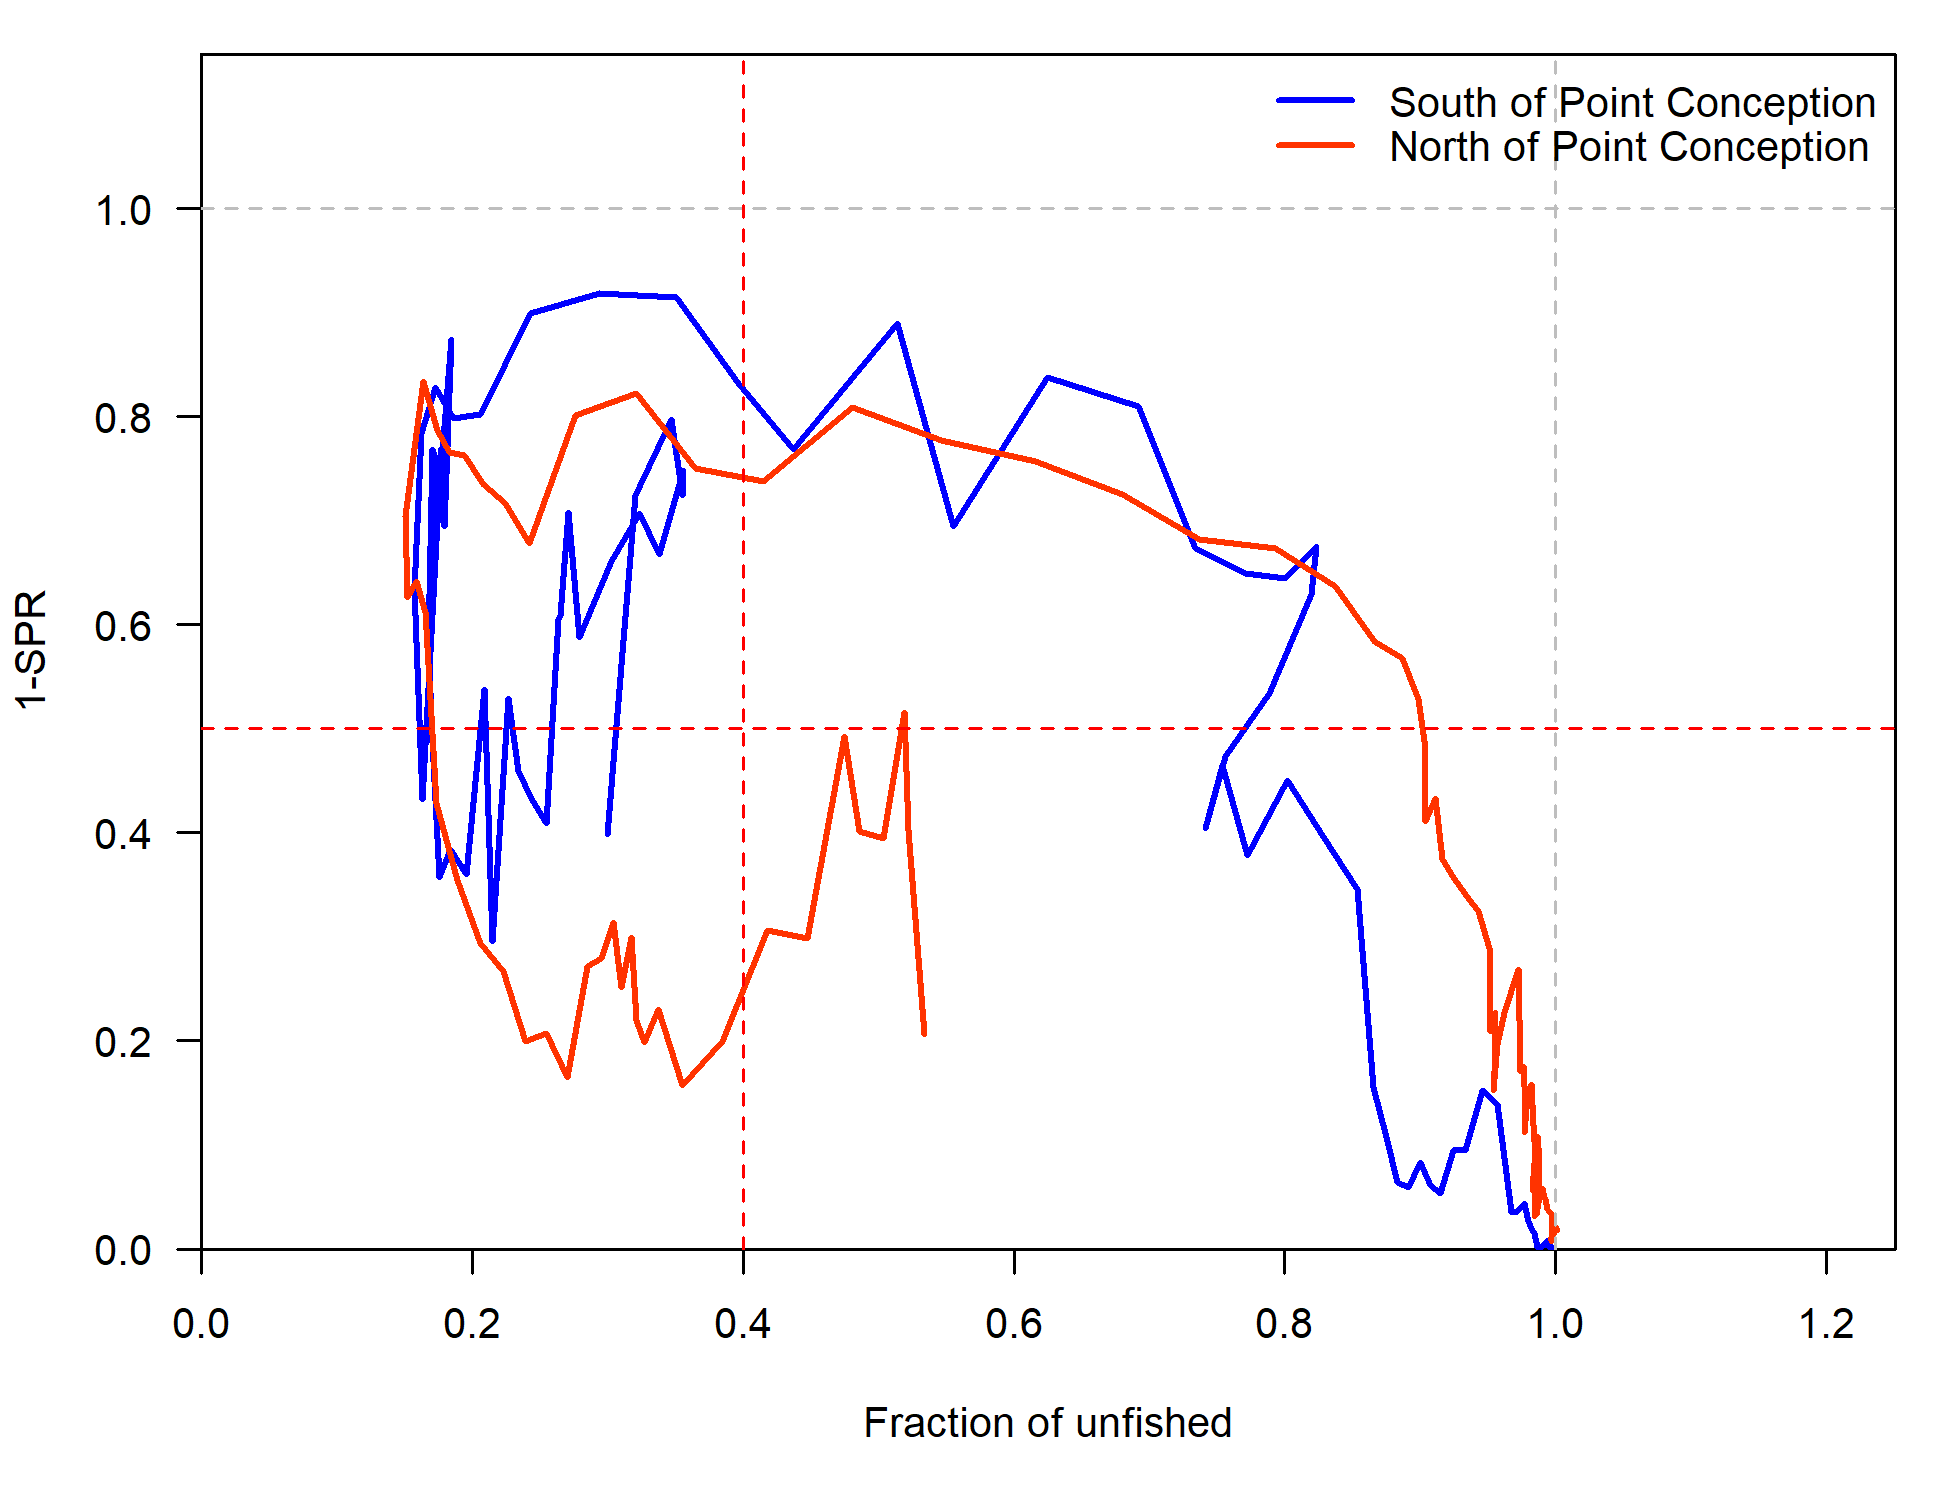
\includegraphics[alt=See Table 22 in this document and Table 15 in the north of Point Conception assessment document.,width=1\textwidth,height=1\textheight]{C:/Users/melissa.monk/Documents/GitHub/copper_rockfish_2023/documents/shared_figures/compare15_phase_plot.png}
}
\caption{Phase plot of estimated 1-SPR versus fraction unfished for the model areas south and north of Point Conception.\label{fig:es-phase}}
\end{figure}

\begin{figure}
{\centering
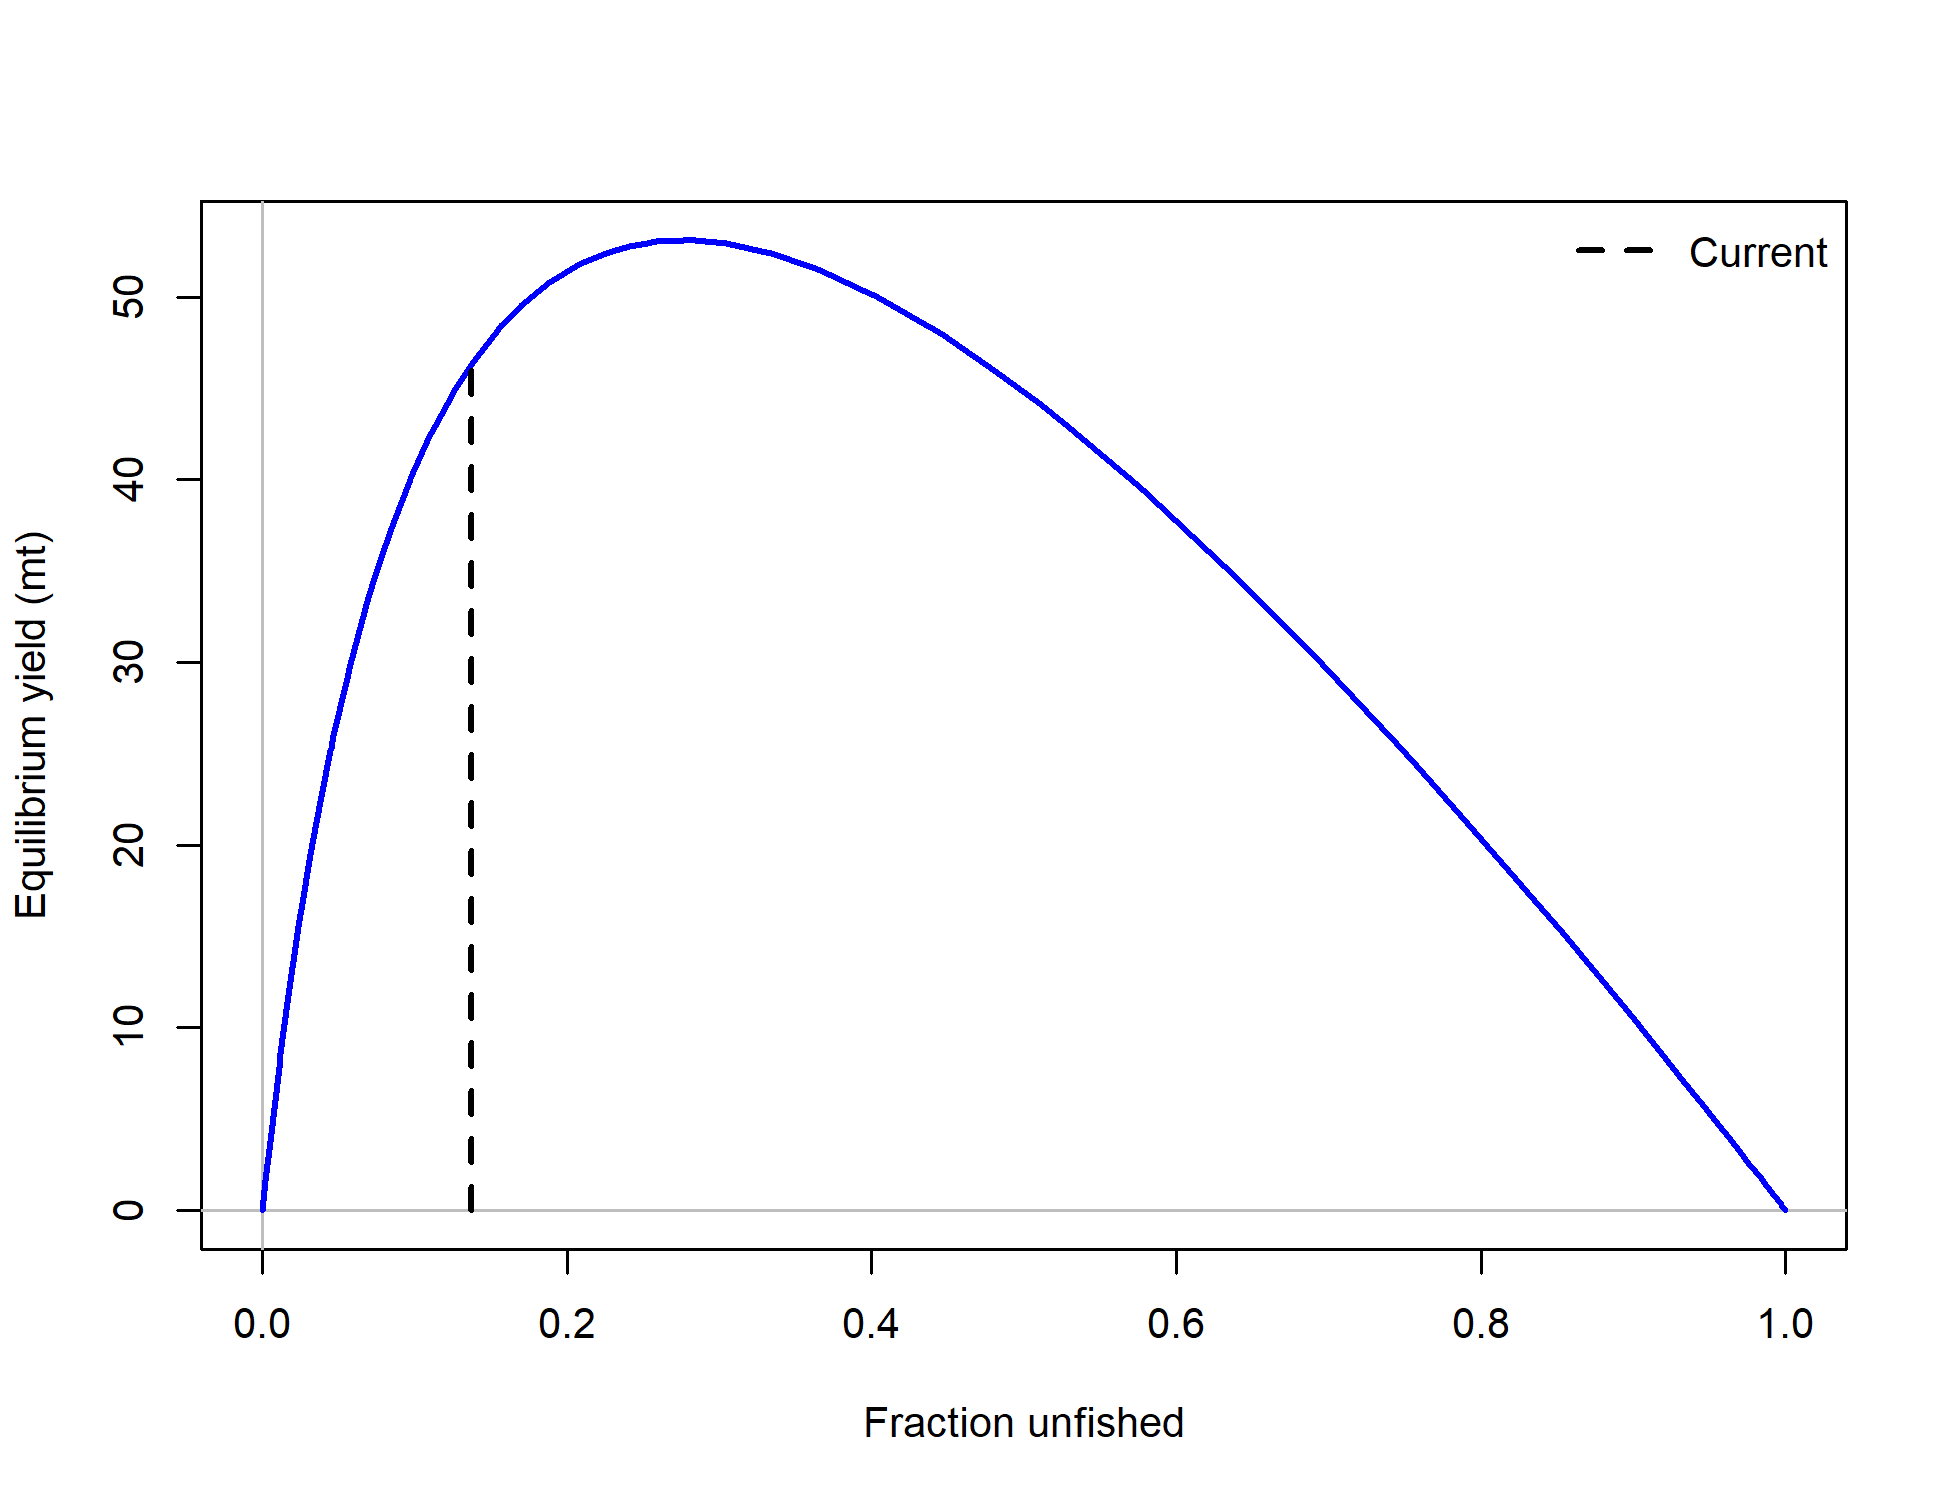
\includegraphics[alt=Equilibrium curve peaks around 0.30 fraction of unfished with the estimated current fraction of unfished at 0.16.,width=1\textwidth,height=1\textheight]{C:/Users/melissa.monk/Documents/GitHub/copper_rockfish_2023/documents/shared_figures/south_yield2_yield_curve_with_refpoints.png}
}
\caption{Equilibrium yield curve for the base case model south of Point Conception. Values are based on the 2022
fishery selectivities and with steepness fixed at 0.72.\label{fig:south-es-yield}}
\end{figure}

\begin{figure}
{\centering
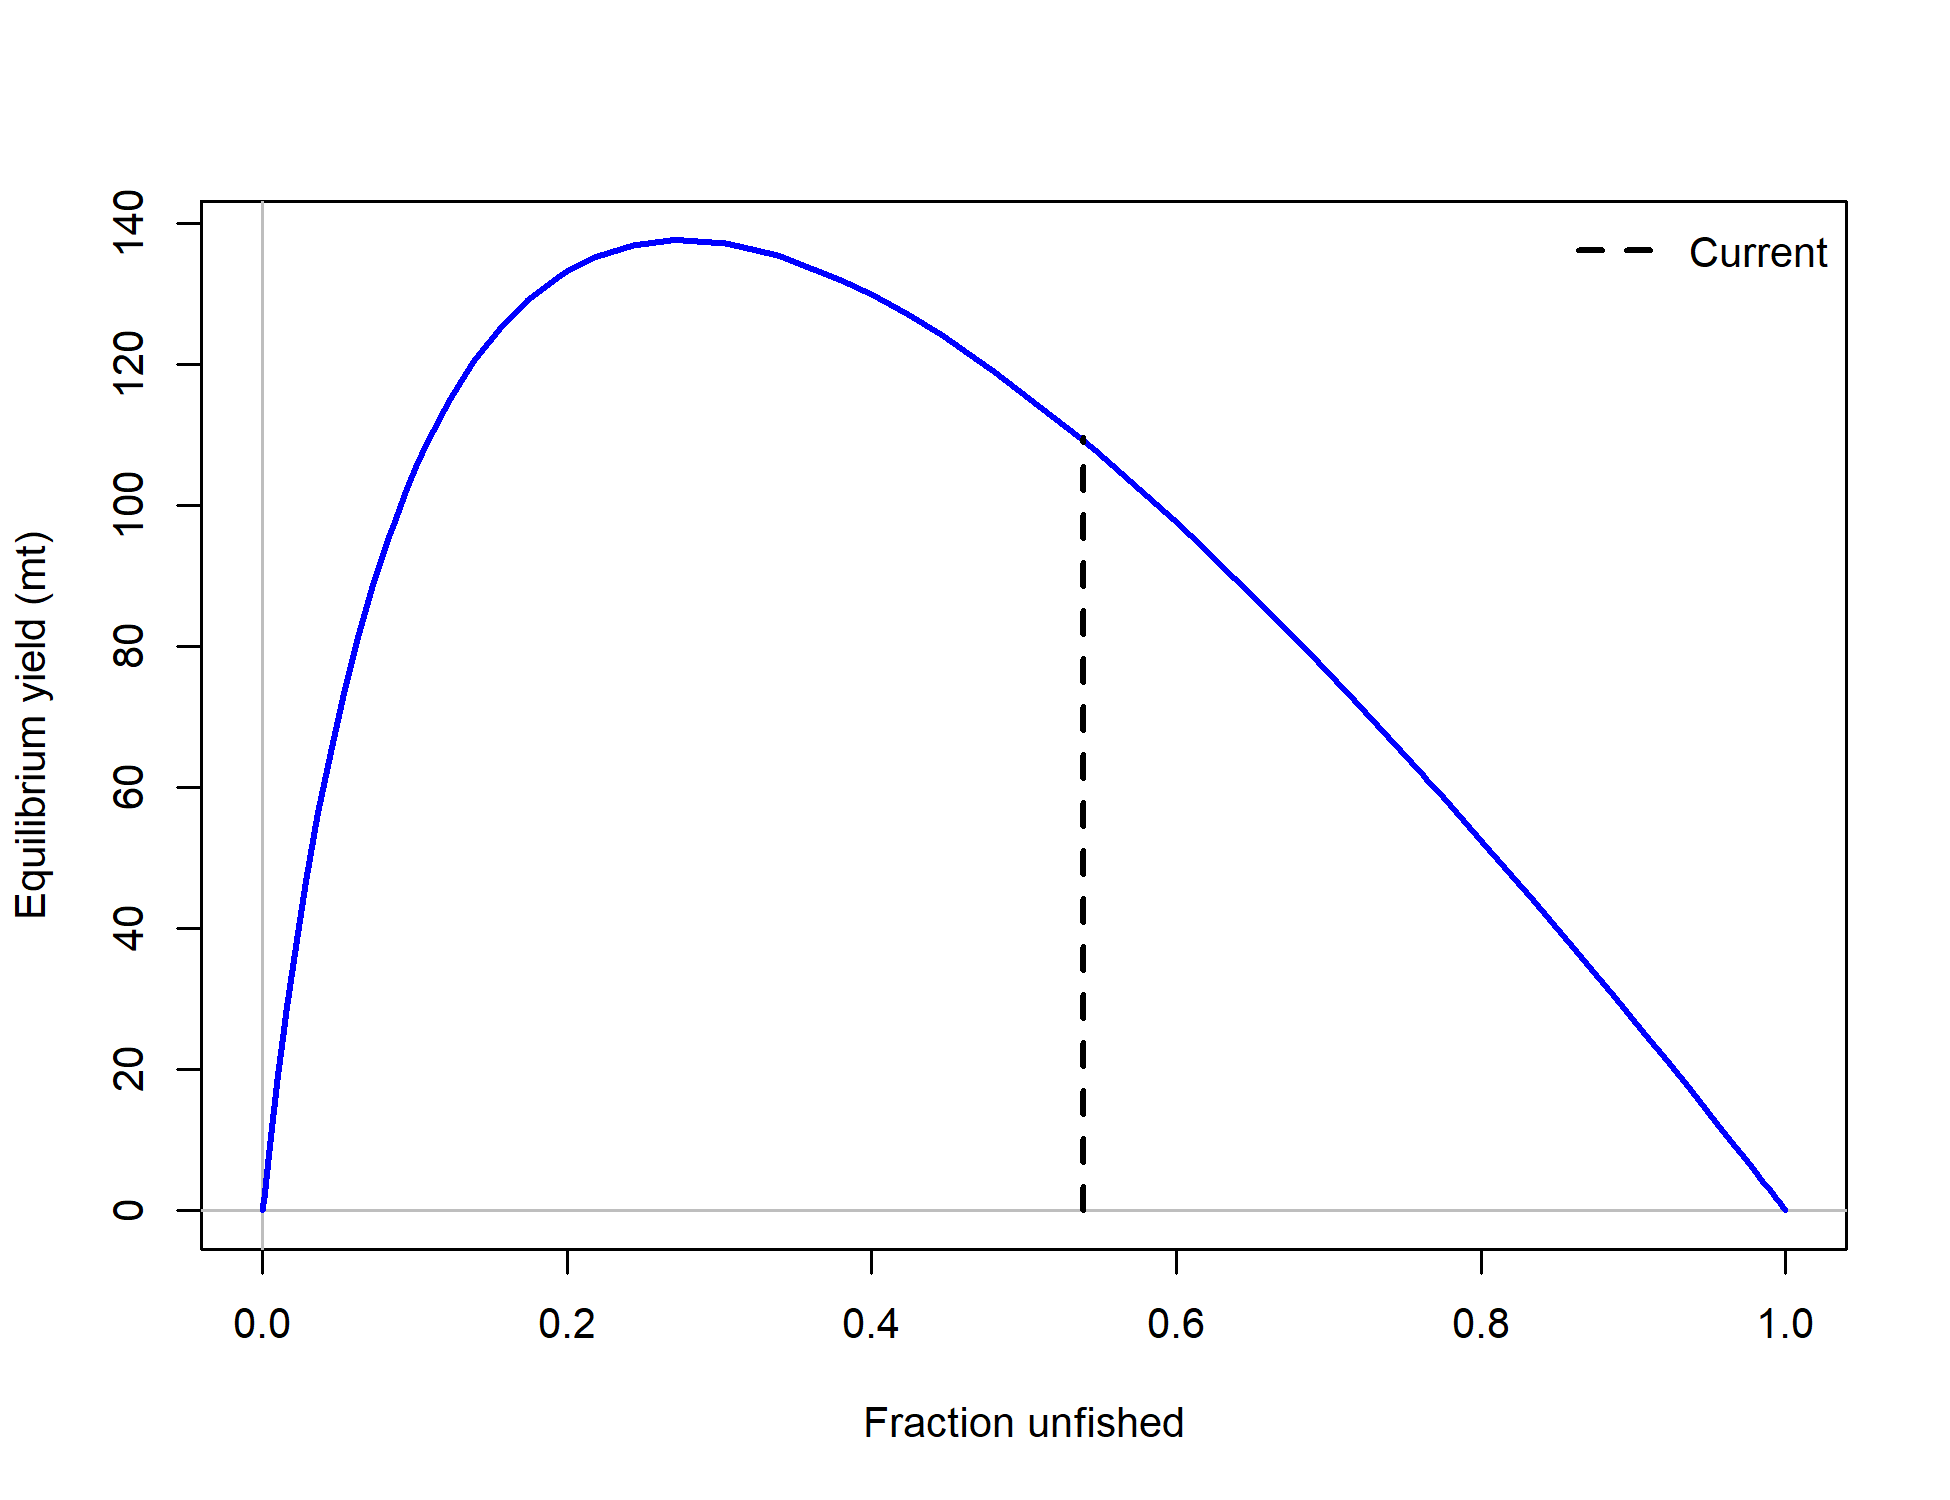
\includegraphics[alt=Equilibrium curve peaks around 0.30 fraction of unfished with the estimated current fraction of unfished at 0.46.,width=1\textwidth,height=1\textheight]{C:/Users/melissa.monk/Documents/GitHub/copper_rockfish_2023/documents/shared_figures/north_yield2_yield_curve_with_refpoints.png}
}
\caption{Equilibrium yield curve for the base case model north of Point Conception. Values are based on the 2022
fishery selectivities and with steepness fixed at 0.72.\label{fig:north-es-yield}}
\end{figure}

\pagebreak

\subsection*{Management performance}\label{management-performance}
\addcontentsline{toc}{subsection}{Management performance}

Copper rockfish are currently managed within two Nearshore Rockfish Complexes, split north and south of 40\(^\circ\) 10' N. lat. The complexes are managed based on overfishing limits (OFL) and annual catch limits (ACL) that are determined by summing the species-specific OFLs and ACLs (ACLs set equal to the Acceptable Biological Catches {[}ABCs{]}) contributions for all stocks managed in the complexes. Limits are shared among all commercial and recreational fleets with the various management procedures intended to maintain removals below the total OFL and ACL for the Nearshore Rockfish north and south complexes as a whole, rather than on a species by species basis.

The species-specific OFL and ACL contribution for copper rockfish that is allocated to California waters, Nearshore Rockfish South and 25 percent of the Nearshore Rockfish North, is shown in Table \ref{tab:es-ca-management} as well as the total catch across California. Over the last ten years the catches of copper rockfish have been below the species-specific ACLs in California. In 2021 all U.S. West Coast stocks of copper rockfish were assessed that informed the 2023-24 harvest specifications species-specific OFLs and ACLs. In California waters the new OFLs and ACLs for the 2023-24 management cycle were significantly lower than early years, resulting in in-season management action by CDFW for 2022 to reduce removals based on the latest stock assessment.

\begingroup\fontsize{10}{12}\selectfont
\begingroup\fontsize{10}{12}\selectfont

\begin{longtable}[t]{c>{\centering\arraybackslash}p{2cm}>{\centering\arraybackslash}p{2cm}>{\centering\arraybackslash}p{2cm}}
\caption{\label{tab:es-ca-management}The species-specific Overfishing Limit (OFL) and Annual Catch Limit (ACL) allocated to California and the total catch (mt) in California waters by year.}\\
\toprule
Year & OFL (mt) & ACL (mt) & Catch (mt)\\
\midrule
\endfirsthead
\caption[]{The species-specific Overfishing Limit (OFL) and Annual Catch Limit (ACL) allocated to California and the total catch (mt) in California waters by year. (\textit{continued)}}\\
\toprule
Year & OFL (mt) & ACL (mt) & Catch (mt)\\
\midrule
\endhead

\endfoot
\bottomrule
\endlastfoot
2012 & 163.2 & 136.2 & 86.0\\
2013 & 148.0 & 123.4 & 105.2\\
2014 & 148.0 & 123.4 & 98.7\\
2015 & 303.8 & 277.3 & 147.6\\
2016 & 286.9 & 262.0 & 165.3\\
2017 & 313.7 & 286.4 & 225.5\\
2018 & 319.6 & 291.8 & 203.7\\
2019 & 325.1 & 296.8 & 182.6\\
2020 & 330.4 & 301.6 & 173.4\\
2021 & 249.8 & 206.4 & 127.8\\
2022 & 249.5 & 204.0 & 66.7\\*
\end{longtable}
\endgroup{}
\endgroup{}

\subsection*{Unresolved problems and major uncertainties}\label{unresolved-problems-and-major-uncertainties}
\addcontentsline{toc}{subsection}{Unresolved problems and major uncertainties}

This assessment models the sub-areas north and south of Point Conception as separate non-mixing sub-populations, but there is likely larval or juvenile dispersal, and potentially some adult movement among these areas. Dispersal and movement rates are not well known. Improved understanding around the dispersal rates of copper rockfish across California, particularly around Point Conception, are needed to support spatial modeling of the stock.

The primary fishery-independent survey for West Coast groundfish, the Northwest Fisheries Science Center (NWFSC) West Coast Groundfish Bottom Trawl (WCGBT) survey, does not sample rocky habitats where most copper rockfish are found, and thus does not provide a robust index of abundance. An alternative survey, the CCFRP Hook and Line survey, provides a reasonable signal for copper rockfish, including relative abundance and demographic structure inside and outside a number of Marine Protect Areas (MPAs).

Age data are limited and consequently growth estimates are uncertain and the available age data contained little to no information to support the estimation of natural mortality. There is some tension among limited data sources and types inferred by the likelihood profiles, with age data suggesting a higher natural mortality rate and length data suggesting a lower value, particularly for the area north of Point Conception. Conflicting signals in the information between length and age data is commonly encountered for many West Coast groundfish stock assessments. The mechanisms driving these differences are uncertain.

Each of the sub-area models estimates high recruitment events over the most recent decade, especially relative to previous time periods. The base model for the sub-area north of Point Conception estimated overall lower variation in recruitment relative to the model south of Point Conception. Oceanographic conditions likely drive periods of either poor or above average recruitment, particularly for rockfish species. However, it is unclear what conditions may be contributing to the differing levels of recruitment variation across the California coast.

\subsection*{Decision table and projections}\label{decision-table-and-projections}
\addcontentsline{toc}{subsection}{Decision table and projections}

Both sub-area models for the California stock of copper rockfish was assigned a category 1 determination by the Scientific and Statistical Committee to the PFMC. A ten-year projection using the combined estimates from each sub-area base model, south and north of Point Conception in California, with catches equal to the estimated Annual Catch Limit (ACL) based on the category 1 time-varying \(\sigma\) with \(P^*\) = 0.45 for years 2025-2034 is shown in Table \ref{tab:es-ca-proj} (i.e., termed the ``buffer''). The removals in 2023 and 2024 were set equal to the portion of copper rockfish species-specific adopted ACLs for California determined by summing the adopted ACLs south of $40^\circ 10^\prime$ N. lat. and the portion of the north of $40^\circ 10^\prime$ N. lat. allocated to California (25 percent - PFMC Groundfish Management Team pers. comm.). The portion of ACL to allocate to each sub-area for 2023-24 was determined based on the proportion of the total removals by area in 2022 (71 percent north and 29 percent south) as recommended by the GMT (Mel Mandrup, CDFW, personal communication). The projections were conducted in an iterative fashion based on the combined estimates of spawning output, relative spawning output, OFL, ABC, and ACL for each year. The estimated proportion of the ACL removed from each sub-area model was based on the proportion of the contribution to the total annual OFL estimate. The allocation of the OFL, ABC, and ACL north and south of $40^\circ 10^\prime$ N. lat. based on the estimates of rocky habitat and the density of copper rockfish in the area are given in Table \ref{tab:es-ca-proj-split}.

At the end of the projection period, 2034, the projected ACL removals result in the California stock increasing to be above the biomass target at percent of the relative spawning output, with the portion of the stock south at 24.5 percent of the sub-area estimated relative spawning output and north of Point Conception at 48.2 percent.

The axes of uncertainty in the decision table are based on the uncertainty around steepness. The estimated uncertainty around the 2023 OFL was used to identify the low and high states of nature that would align with the 12.5 and 87.5 percentiles from the base model where the base model is assigned a 50 percent probability of being the true state of nature and both the low and high states of nature being assigned a 25 percent probability. A search across steepness (\(h\)) values for each sub-area model was conducted to identify the corresponding steepness values that would create the low and high states of nature relative to the base model. The sub-area north of Point Conception applied values of \(h\) of: 0.655, 0.72, and 0.859. The sub-area south of Point Conception applied values of \(h\) of: 0.54, 0.72, and 0.929. The proposed decision table assumes full ACL removal during the projection period under P* alternative catch stream (Table \ref{tab:dec-tab-es}).

\begingroup\fontsize{9}{11}\selectfont

\begin{landscape}\begingroup\fontsize{9}{11}\selectfont

\begin{longtable}[t]{c>{\centering\arraybackslash}p{1.3cm}>{\centering\arraybackslash}p{1.1cm}>{\centering\arraybackslash}p{1.1cm}>{\centering\arraybackslash}p{1.1cm}>{\centering\arraybackslash}p{1.1cm}>{\centering\arraybackslash}p{1.4cm}>{\centering\arraybackslash}p{1.4cm}>{\centering\arraybackslash}p{1.6cm}>{\centering\arraybackslash}p{1.6cm}>{\centering\arraybackslash}p{1.3cm}}
\caption{\label{tab:es-ca-proj}The estimated OFL (mt), ABC (mt), ACL (mt), buffer, spawning output in billions of eggs across California, and relative spawning outut by year along with the sub-area allocations of the ACL south of Point Conception (south, $34^\circ 27^\prime$ N. lat.), north of Point Conception to $40^\circ 10^\prime$ N. lat. (central), and $40^\circ 10^\prime$ to $42^\circ$ N. lat. (north).}\\
\toprule
Year & Assumed Catch (mt) & OFL (mt) & ABC (mt) & ACL (mt) & Buffer & Spawning Output & Fraction Unfished & Sub-ACL South (mt) & Sub-ACL Central (mt) & Sub-ACL North (mt)\\
\midrule
\endfirsthead
\caption[]{The estimated OFL (mt), ABC (mt), ACL (mt), buffer, spawning output in billions of eggs across California, and relative spawning outut by year along with the sub-area allocations of the ACL south of Point Conception (south, $34^\circ 27^\prime$ N. lat.), north of Point Conception to $40^\circ 10^\prime$ N. lat. (central), and $40^\circ 10^\prime$ to $42^\circ$ N. lat. (north). (\textit{continued)}}\\
\toprule
Year & Assumed Catch (mt) & OFL (mt) & ABC (mt) & ACL (mt) & Buffer & Spawning Output & Fraction Unfished & Sub-ACL South (mt) & Sub-ACL Central (mt) & Sub-ACL North (mt)\\
\midrule
\endhead

\endfoot
\bottomrule
\endlastfoot
2023 & 91.5 & - & - & - & - & 240.80 & 0.366 & - & - & -\\
2024 & 94.7 & - & - & - & - & 245.88 & 0.374 & - & - & -\\
2025 & - & 143.5 & 134.1 & 131.9 & 0.935 & 250.60 & 0.381 & 15.8 & 109.2 & 6.8\\
2026 & - & 145.3 & 135.2 & 133.1 & 0.93 & 251.62 & 0.383 & 18 & 108.4 & 6.7\\
2027 & - & 147.2 & 136.3 & 134.5 & 0.926 & 252.91 & 0.385 & 20.1 & 107.7 & 6.7\\
2028 & - & 148.9 & 137.3 & 135.8 & 0.922 & 254.64 & 0.388 & 22 & 107.1 & 6.7\\
2029 & - & 150.4 & 137.9 & 136.7 & 0.917 & 256.75 & 0.391 & 23.5 & 106.6 & 6.6\\
2030 & - & 151.6 & 138.5 & 137.7 & 0.913 & 259.10 & 0.394 & 24.8 & 106.3 & 6.6\\
2031 & - & 152.8 & 138.9 & 138.6 & 0.909 & 261.54 & 0.398 & 26 & 106 & 6.6\\
2032 & - & 153.9 & 139.1 & 139.1 & 0.904 & 264.02 & 0.402 & 27 & 105.6 & 6.6\\
2033 & - & 155 & 139.5 & 139.5 & 0.9 & 266.52 & 0.406 & 27.9 & 105.1 & 6.5\\
2034 & - & 156.2 & 139.9 & 139.9 & 0.896 & 269.04 & 0.409 & 28.8 & 104.6 & 6.5\\*
\end{longtable}
\endgroup{}
\end{landscape}
\endgroup{}

\pagebreak

'

\begingroup\fontsize{10}{12}\selectfont
\begingroup\fontsize{10}{12}\selectfont

\begin{longtable}[t]{c>{\centering\arraybackslash}p{1.3 cm}>{\centering\arraybackslash}p{1.3 cm}>{\centering\arraybackslash}p{1.3 cm}>{\centering\arraybackslash}p{1.3 cm}>{\centering\arraybackslash}p{1.3 cm}>{\centering\arraybackslash}p{1.3 cm}>{\centering\arraybackslash}p{1.3 cm}}
\caption{\label{tab:es-ca-proj-split}The estimated California OFL (mt), ABC (mt), and ACL (mt) split south and north $40^\circ 10^\prime$ N. lat. The estimated percent allocated to the north $40^\circ 10^\prime$ N. lat. in California is 5.86 percent based on estimates of rocky habitat and density of copper rockfish in the area.}\\
\toprule
Year & Assumed Catch (mt) & South OFL (mt) & South ABC (mt) & South ACL (mt) & North OFL (mt) & North ABC (mt) & North ACL (mt)\\
\midrule
\endfirsthead
\caption[]{The estimated California OFL (mt), ABC (mt), and ACL (mt) split south and north $40^\circ 10^\prime$ N. lat. The estimated percent allocated to the north $40^\circ 10^\prime$ N. lat. in California is 5.86 percent based on estimates of rocky habitat and density of copper rockfish in the area. (\textit{continued)}}\\
\toprule
Year & Assumed Catch (mt) & South OFL (mt) & South ABC (mt) & South ACL (mt) & North OFL (mt) & North ABC (mt) & North ACL (mt)\\
\midrule
\endhead

\endfoot
\bottomrule
\endlastfoot
2023 & 91.5 & - & - & - & - & - & -\\
2024 & 94.7 & - & - & - & - & - & -\\
2025 & - & 136.06 & 127.22 & 125.08 & 7.4 & 6.92 & 6.8\\
2026 & - & 137.97 & 128.31 & 126.33 & 7.37 & 6.85 & 6.75\\
2027 & - & 139.91 & 129.55 & 127.79 & 7.34 & 6.8 & 6.7\\
2028 & - & 141.63 & 130.58 & 129.11 & 7.32 & 6.74 & 6.67\\
2029 & - & 143.09 & 131.21 & 130.1 & 7.3 & 6.69 & 6.64\\
2030 & - & 144.36 & 131.8 & 131.1 & 7.28 & 6.65 & 6.61\\
2031 & - & 145.53 & 132.28 & 131.99 & 7.28 & 6.61 & 6.6\\
2032 & - & 146.65 & 132.57 & 132.57 & 7.27 & 6.57 & 6.57\\
2033 & - & 147.77 & 132.99 & 132.99 & 7.27 & 6.54 & 6.54\\
2034 & - & 148.92 & 133.43 & 133.43 & 7.27 & 6.51 & 6.51\\*
\end{longtable}
\endgroup{}
\endgroup{}

\pagebreak

\begingroup\fontsize{9}{11}\selectfont
\begingroup\fontsize{9}{11}\selectfont

\begin{longtable}[t]{l>{\raggedright\arraybackslash}p{0.8cm}>{\raggedright\arraybackslash}p{0.8cm}>{\raggedright\arraybackslash}p{1.45cm}>{\raggedright\arraybackslash}p{1.45cm}>{\raggedright\arraybackslash}p{1.45cm}>{\raggedright\arraybackslash}p{1.45cm}>{\raggedright\arraybackslash}p{1.45cm}>{\raggedright\arraybackslash}p{1.45cm}}
\caption{\label{tab:dec-tab-es}Decision table summary of 10-year projections beginning in 2025 for alternative states of nature based on an axis of uncertainty around steepness for both California sub-area models. The spawning output and depletion is for the whole California stock with the annual projected catch removed from each sub-area model equal to the contribution proportion for each sub-area OFL. Columns range over low, mid, and high states of nature and rows range over different catch P* values. The removals in 2023 and 2025 are set equal to the adopted ACL for the California stock.}\\
\toprule
\multicolumn{3}{c}{ } & \multicolumn{2}{c}{Low Steepness} & \multicolumn{2}{c}{Base Steepness} & \multicolumn{2}{c}{High Steepness} \\
\cmidrule(l{3pt}r{3pt}){4-5} \cmidrule(l{3pt}r{3pt}){6-7} \cmidrule(l{3pt}r{3pt}){8-9}
  & Year & Catch & Spawning Output & Fraction Unfished & Spawning Output & Fraction Unfished & Spawning Output & Fraction Unfished\\
\hline
&	2023	&	91.5	&	176.2	&	0.255	&	240.8	&	0.366	&	337.3	&	0.533	\\
&	2024	&	94.7	&	178.2	&	0.258	&	245.9	&	0.374	&	345.7	&	0.546	\\
&	2025	&	131.9	&	180.2	&	0.261	&	250.6	&	0.381	&	352.9	&	0.558	\\
&	2026	&	133.1	&	178.9	&	0.259	&	251.6	&	0.382	&	355.4	&	0.562	\\
&	2027	&	134.5	&	178.2	&	0.258	&	252.9	&	0.384	&	357.3	&	0.564	\\
ACL	&	2028	&	135.8	&	178.0	&	0.258	&	254.6	&	0.387	&	358.9	&	0.567	\\
P* 0.45	&	2029	&	136.7	&	178.3	&	0.258	&	256.7	&	0.390	&	360.4	&	0.569	\\
&	2030	&	137.7	&	178.9	&	0.259	&	259.1	&	0.394	&	361.8	&	0.572	\\
&	2031	&	138.6	&	179.6	&	0.260	&	261.5	&	0.397	&	363.1	&	0.574	\\
&	2032	&	139.1	&	180.4	&	0.261	&	264.0	&	0.401	&	364.3	&	0.575	\\
&	2033	&	139.5	&	181.2	&	0.262	&	266.5	&	0.405	&	365.3	&	0.577	\\
&	2034	&	139.9	&	182.0	&	0.264	&	269.0	&	0.409	&	366.2	&	0.578	\\
\hline																	
&	2023	&	91.5	&	176.2	&	0.255	&	240.8	&	0.366	&	337.3	&	0.533	\\
&	2024	&	94.7	&	178.2	&	0.258	&	245.9	&	0.374	&	345.7	&	0.546	\\
&	2025	&	123.1	&	180.2	&	0.261	&	250.6	&	0.381	&	352.9	&	0.558	\\
&	2026	&	124.2	&	179.7	&	0.260	&	252.4	&	0.384	&	356.3	&	0.563	\\
&	2027	&	125.4	&	179.9	&	0.261	&	254.6	&	0.387	&	359.1	&	0.567	\\
ACL	&	2028	&	126.5	&	180.7	&	0.262	&	257.3	&	0.391	&	361.6	&	0.571	\\
P* 0.40	&	2029	&	127.4	&	181.9	&	0.263	&	260.3	&	0.396	&	364.1	&	0.575	\\
&	2030	&	128.1	&	183.4	&	0.266	&	263.6	&	0.401	&	366.4	&	0.579	\\
&	2031	&	128.2	&	185.1	&	0.268	&	267.1	&	0.406	&	368.7	&	0.582	\\
&	2032	&	128.4	&	186.9	&	0.271	&	270.6	&	0.411	&	370.8	&	0.586	\\
&	2033	&	128.4	&	188.8	&	0.273	&	274.1	&	0.416	&	372.8	&	0.589	\\
&	2034	&	128.5	&	190.7	&	0.276	&	277.7	&	0.422	&	374.7	&	0.592	\\
\hline																	
&	2023	&	91.5	&	176.2	&	0.255	&	240.8	&	0.366	&	337.3	&	0.533	\\
&	2024	&	94.7	&	178.2	&	0.258	&	245.9	&	0.374	&	345.7	&	0.546	\\
&	2025	&	114.7	&	180.2	&	0.261	&	250.6	&	0.381	&	352.9	&	0.558	\\
&	2026	&	115.6	&	180.5	&	0.261	&	253.3	&	0.385	&	357.1	&	0.564	\\
ACL	&	2027	&	116.7	&	181.5	&	0.263	&	256.3	&	0.389	&	360.7	&	0.570	\\
P* 0.35	&	2028	&	117.5	&	183.2	&	0.265	&	259.8	&	0.395	&	364.2	&	0.575	\\
&	2029	&	118.2	&	185.3	&	0.268	&	263.8	&	0.401	&	367.6	&	0.581	\\
&	2030	&	118.1	&	187.8	&	0.272	&	268.1	&	0.407	&	370.9	&	0.586	\\
&	2031	&	118.0	&	190.5	&	0.276	&	272.5	&	0.414	&	374.1	&	0.591	\\
&	2032	&	117.9	&	193.4	&	0.280	&	277.0	&	0.421	&	377.2	&	0.596	\\
&	2033	&	117.6	&	196.3	&	0.284	&	281.5	&	0.428	&	380.2	&	0.601	\\
&	2034	&	117.4	&	199.2	&	0.289	&	286.1	&	0.435	&	383.1	&	0.605	\\*
 \hline
\end{longtable}
\endgroup{}
\endgroup{}


\pagebreak

\subsection*{Scientific uncertainty}\label{scientific-uncertainty}
\addcontentsline{toc}{subsection}{Scientific uncertainty}

The model estimated uncertainty around the 2023 spawning output for the sub-area model south of Point Conception is \(\sigma\) = 0.3 and the uncertainty for the sub-area model north of Point Conception is \(\sigma\) = 0.31. The uncertainty around the OFL south and north of Point Conception was \(\sigma\) = 0.28 and 0.3, respectively. Each of these are likely underestimates of overall uncertainty due to the necessity to fix several key population dynamics parameters (e.g., steepness, recruitment variance, natural mortality) and also because there is no explicit incorporation of model structural uncertainty (although see the decision table for alternative states of nature).

\subsection*{Research and data needs}\label{research-and-data-needs}
\addcontentsline{toc}{subsection}{Research and data needs}

There were some major sources of uncertainty within the assessments for copper rockfish. To improve our understanding of the copper rockfish stock in California waters the following research and data collection should be prioritized:

\begin{enumerate}

    \item  The NWFSC Hook and Line survey is the only long-term fishery-independent survey in rocky (untrawlable) habitat in the Southern California Bight. Efforts should continue to explore how best to model hook and line catch data to develop indices of abundance. We also recommend evaluating how to structure the NWFSC Hook and Line survey index, given its expansion into the CCAs and increase in sites within designated MPAs, and independent analysis of information content in NWFSC Hook and Line survey across observed species. Finally, increased spatiotemporal sampling around Point Conception would aid in identifying stock boundaries.

    \item The assessment area south of Point Conception appears to have a mixture of observations from areas experiencing variable fishing mortality. In the region there are likely a mixture of areas: open access rocky reefs that are close to port that are heavily fished, open access rocky reefs that are inaccessible via day-trips that are fished but likely at lower levels, and rocky reefs that fall within marine protected areas (MPAs). A spatially-explicit assessment model may be able to capture this complexity but will require data (indices of abundance and composition data) from each of the regions. 
    
    \item Future nearshore assessments would greatly benefit from additional CDFW ROV surveys which could increase the power of these data to inform assessments.

    \item There are very limited age data for copper rockfish across California arising from fishery-dependent sources. Establishing regular collections of otoliths from the recreational fishery, a large source of mortality, would support future assessments and would improve the understanding of the population structure and life history of copper rockfish. 

    \item There is limited information for copper rockfish on maturity and fecundity and the variability of these parameters with increasing latitude.  The NWFSC WCGBT and Hook and Line surveys provided the only available information on the maturity ogive and the timing of these surveys does not overlap with the expected peak spawning season. The Southwest Fisheries Science Center has egg samples from a total of ten copper rockfish, which is too few to draw conclusions regarding fecundity.

    \item Some of the PR mode recreational data that should be available via RecFIN were found to contain information in that database inconsistent with datasheets available from CDFW. There is also a question if length data collected by the Deb Wilson-Vandenberg onboard observer survey is duplicated within RecFIN and attributed to MRFSS dockside samples of the CPFV fleet.

    \item The interpreted substrate data for the areas north of Point Conception within state waters is incomplete. Additional data needs include high resolution interpreted substrate maps for areas outside of state waters. The available interpreted bathymetry data from south of Point Conception is incomplete within state waters  around the northern and southern Channel Islands. This poses a challenge for estimating available rocky substrate both by district and also inside and outside closed areas. 

    \item The genetic stock structure of copper rockfish warrants further investigation to ensure appropriate management of copper rockfish along the West Coast. 

    \item The Marine Recreational Fisheries Statistics Survey (MRFSS) index was excluded from both California assessment models. The standardized trends in abundance were marked by extreme peaks in the data throughout the time series. The STAT was unable to identify what may driving extreme changes fishing behavior in these select years. These data should be reviewed to better understand whether these data reflect true changes in fishing behavior in those years or errors in data collection. 

    \item Additional research on the effect of the MPA network on copper rockfish and other nearshore rockfish species needs to be conducted. The trend inside the MPAs in northern California exhibited an increasing trend compared to outside the MPAs, similar to what was observed during the 2021 assessment of vermilion/sunset rockfish. However, the trends inside MPAs south of Point Conception varied by location with a number of sites showing flat or declining trends.  

    \item Further investigations of other available fishery-independent data such as the Partnership for Interdisciplinary Studies of Coastal Oceans (PISCO) kelp forest index would benefit future assessments of nearshore species, including copper rockfish. 

    \item Larval and smaller young-of-the-year copper rockfish can only be identified with certainty genetically. Existing sources of data (CalCOFI and Standard Monitoring Units for the Recruitment of Fishes [SMURFs]) where genetic samples can be analyzed would provide key information to inform spawning output estimates for copper rockfish.
 
    \item Continue to improve historical catch reconstructions, including attempting to quantify uncertainty with these and other historical data.
  
    \item Existing catch estimates within Recreational Fisheries Information Network (RecFIN) that are currently assigned only to "rockfish, general" should be investigated to determine if these removals can be assigned to specific species.

\end{enumerate}

\pagebreak
\setlength{\parskip}{5mm plus1mm minus1mm}
\pagenumbering{arabic}
\setcounter{page}{1}
\renewcommand{\thefigure}{\arabic{figure}}
\renewcommand{\thetable}{\arabic{table}}
\setcounter{table}{0}
\setcounter{figure}{0}

\section{Introduction}\label{introduction}

This assessment report describes the sub-area population of copper rockfish (\emph{Sebastes caurinus}) off the California coast north of Point Conception in U.S. waters, using data through 2022 (Figure \ref{fig:ca-map}). The sub-area population south of Point Conception in California waters was also evaluated and is described in a separate assessment report. The copper rockfish status for the California stock is determined by the combined estimates of spawning output from both sub-areas and is detailed in the \hyperref[management]{management} Section. This assessment does not account for populations located in Mexican waters or other areas off the U.S. West Coast and assumes that these southern and northern populations do not contribute to nor take from the population being assessed here.

\subsection{Basic Information and Life History}\label{basic-information-and-life-history}

Copper rockfish have historically been a part of both commercial and recreational fisheries throughout its range. Copper rockfish are a demersal, relatively nearshore species within the subgenus \emph{Pteropodus.} The core range of copper rockfish is comparatively large, ranging from northern Baja Mexico to the Gulf of Alaska, with copper rockfish also found in Puget Sound. Copper rockfish range from the sub-tidal (as juveniles) to depths of around 180 m (Love et al. 2002). Copper rockfish are commonly found in waters less than 100 m in depth inhabiting nearshore kelp forests and complex low-relief rocky habitat (Love 1996). Adult copper rockfish have high site fidelity and are thought to not make long-range movements. An acoustic telemetry study displaced copper rockfish 4 km from their capture location to an artificial reef and within 10 days, half of the copper rockfish returned to the original capture location (Reynolds et al. 2010).

Copper rockfish have a clearly defined long white band the posterior two-thirds of the lateral line. Copper rockfish have high variation in coloration throughout its range, taking on coloration from dark brown, olive, orange-red and pink, with patches of yellow and pink (Miller and Lea 1972). In general, the copper rockfish towards the northern part of the range are often darker in color than fish encountered in southern California. The distinct change in coloration resulted in copper rockfish initially being described as two separate species, copper rockfish (\emph{S. caurinus}) and whitebelly rockfish (\emph{S. vexillaris}).

The \emph{Sebastes} genus is viviparous with internal fertilization, many species exhibit dimorphic growth with females larger at size-at-age than males, and a number of species have reproductive strategies that vary with latitude. There are very few fecundity samples from copper rockfish available from California, although copper rockfish are assumed to produce a single brood annually during the winter months.

The pelagic larvae are encountered in the California Cooperative Oceanic Fisheries Investigations (CalCOFI) surveys, but neither larval nor young-of-the-year can be identified visually (Thompson et al. 2017). The size at birth ranges from 5-6 mm and the larvae remain pelagic until approximately 22-23 mm standard length at which time they recruit to the kelp forest canopy (Anderson 1983).

Juvenile copper rockfish are indistinguishable from kelp (\emph{S. atrovirens}), black-and-yellow (\emph{S. chrysomelas}), and gopher (\emph{S. carnatus}) rockfishes, all of which recruit to the kelp forest canopy in the spring months. Copper rockfish is the first of the species group to recruit to the kelp forest from April to May and can be distinguished from the other species once it reaches a size around 5 cm standard length (Anderson 1983). Baetscher et al. (2019) genetically identified young-of-the-year rockfish from surveys in Carmel and Monterey Bays in California and provided the authors with the length and genotyped species identifications from her study. The average total length of young-of-the-year copper rockfish in July was 3-4 cm (Figure \ref{fig:copper-smurf-length}). Anderson (1983) observed benthic copper rockfish nocturnally active over sandy bottom outside the kelp forest.

Copper rockfish are a relatively long-lived rockfish, estimated to live at least 50 years (Love 1996). Copper rockfish were determined to have the highest vulnerability (V = 2.27) of any West Coast groundfish stock evaluated in a productivity susceptibility analysis (Cope et al. 2011). This analysis calculated species-specific vulnerability scores based on two dimensions: productivity characterized by the life history and susceptibility that characterized how the stock could be impacted by fisheries and other activities.

Copper rockfish are opportunistic carnivores and commonly consume crustaceans, mollusks, and fish whole (Lea et al. 1999; Bizzarro et al. 2017). Prince (1972) observed a shift in a diet dominated by arthropods in age 0 and 1 fish to a more diverse diet including molluscs and fish as they aged. The study also noted that juvenile copper rockfish were preyed upon by harbor seals and lingcod. Two tagging studies of copper rockfish indicated that most individuals have a small home range, with 91 percent of recaptures from CCFRP (unpublished data) and 49 percent of individuals from Hanan (2012) within 1 km (straight line distance) of the original release site. Of the 117 recaptures from Hanan (2012), four traveled greater than 50 km, with a maximum distance of 488 km (1,222 days at liberty), and four individuals crossed the biogeographic boundary of Point Conception. Of the 133 copper rockfish recaptures from CCFRP, four traveled greater than 50 km, and the maximum distance traveled was 169 km by two different fish (291 and 524 days at liberty).

There is currently little evidence of significant stock structure from genetic studies of copper rockfish across the west coast. Buonaccorsi et al. (2002) looked at genetic variation across six micosatellite DNA loci from samples ranging from British Columbia to southern California. Significant population subdivision was detected between the Puget Sound and coastal samples which supports the model of isolation-by-distance for copper rockfish. Sivasundar and Palumbi (2010) conducted a genetic study to determine the potential for biogeographic boundaries to prohibit gene flow for 15 \emph{Sebastes} species. The study included 45 observations of copper rockfish with samples from Oregon (N = 18), Monterey Bay (N = 18), and Santa Barbara (N = 9). Sivasundar and Palumbi (2010) used mtDNA and could differentiate samples from Santa Barbara from those collected in Oregon and Monterey Bay, but the Monterey Bay and Oregon samples could not be distinguished. Micosatellite data did not reveal any genetic differentiation among the samples from the three locations for copper rockfish and suggests low genetic differentiation coastwide. An earlier genetic analysis of copper rockfish was conducted by Johansson et al. (2008). The study included 749 samples from along the west coast ranging from Neah Bay, Washington to San Diego, California with the majority of sampling locations clustered north of Cape Mendocino in northern California. The study included 185 samples collected within California. Eleven microsatellite DNA loci were analyzed. The study found significant evidence to support isolation by distance at the coast wide scale. Weak, but significant, genetic structure was identified from samples collected along the Oregon coast suggesting that habitat barriers may limit larval dispersal.

\subsection{Ecosystem Considerations}\label{ecosystem-considerations-1}

This stock assessment does not explicitly incorporate trophic interactions, habitat factors (other than as they inform relative abundance indices) or environmental factors into the assessment model, but a brief description of likely or potential ecosystem considerations is provided below.

As with most other rockfish and groundfish in the California Current, recruitment or cohort (year-class) strength appears to be highly variable for copper rockfish, with only a modest apparent relationship to estimated levels of spawning output. Oceanographic and ecosystem factors are widely recognized to be key drivers of recruitment variability for most species of groundfish, as well as most elements of California Current food webs. Empirical estimates of recruitment from pelagic juvenile rockfish surveys have been used to inform incoming year class strength for some of these stocks, however copper rockfish are infrequently encountered in these surveys. Between 1998 and 2013 the California Cooperative Oceanic Fisheries Investigation (CalCOFI) survey had 34 positive observations of copper rockfish out of over 500 bongo net tows.

\subsection{Historical and Current Fishery Information}\label{historical-and-current-fishery-information}

Off the coast of California north of Point Conception, copper rockfish is caught in both commercial and recreational fisheries. Recreational removals have been the largest source of fishing mortality of copper rockfish across all years (Table \ref{tab:allcatches} and Figure \ref{fig:catch}). The recreational fishery is comprised of individual recreational fishers (Private/Rental, PR) and commercial passenger fishing vessels (CPFV) also known as party/charter (PC) which take groups of individuals out for day fishing trips. Across both types of recreational fishing, the majority of effort occurs around rocky reefs that can be accessed via day-trips.

The recreational fishery in the early part of the 20th century was focused on nearshore waters near ports, with expanded activity further from port and into deeper depths over time (Miller et al. 2014). Prior to the groundfish fishery being declared a federal disaster in 2000, and the subsequent rebuilding period, there were no time or area closures for groundfish. Access to deeper depths during this period spread effort over a larger area and filled bag limits with a greater diversity of species from both the shelf and nearshore. This resulted in lower catch of nearshore rockfish relative to the period after 2000. Between 1999 and 2002, gear regulations went from unlimited hooks and lines to one line per person with no more than two hooks, the current 10 rockfish, cabezon, greenling (RCG) bag limit was enacted, and CDFW created management areas to restrict fishing shoreward of the 20 to 60 fathoms (fm). Depth restrictions ranged from 20 fm in the Northern Management Area (California/Oregon Border to $40^\circ 10^\prime$ N. lat.) to 60 fm in the Southern Management Area (south of Point Conception, $34^\circ 27^\prime$ N. lat.). The latitudinal boundaries of the management areas and depth closures have fluctuated since 2002, but have remained fairly consistent since 2011. This shifting effort onto the nearshore, concomitantly increased catch rates for nearshore rockfish including copper rockfish in the remaining open depths. California's network of Marine Protected Areas (MPAs) also closed approximately 20 to 27 percent of state waters to recreational fishing, with the majority of MPAs developed in 2007.

The depth restrictions have slowly been relaxed following the rebuilding of all previously overfished groundfish species as of 2019, other than yelloweye rockfish (\emph{S. ruberrimus}). The Southern Management area gained access to a depth of 75 fm in 2019, and out to 100 fm in 2021 and 2022. To the north of Point Conception, where yelloweye rockfish are more prevalent, depth constraints persist with most northern areas limited to 30 fm and shallower and more southern areas limited to fishing 50 fm and shallower through 2022. The recreational regulations for 2023 differ from the most recent years and are described in the management section.

Prior to development of the live fish market in the 1980s, there was very little commercial catch of copper rockfish, with dead copper rockfish yielding a low ex-vessel price per pound. Copper rockfish were targeted along with other rockfish to some degree in the nearshore or caught as incidental catch by vessels targeting other more valuable stocks such as lingcod. Most fish were caught using hook and line gear, though some were caught using traps, gill nets and, rarely, trawl gear. Trawling was prohibited within three miles of shore in 1953 and gill netting within three miles of shore was prohibited in 1994, preventing access to a high proportion of the species habitat with these gear types.

In the late 1980s and early 1990s a market for fish landed live arose out of Los Angeles and the San Francisco Bay area, driven by demand from Asian restaurants and markets. The growth of the live fish market was driven by consumers willing to pay a higher price for live fish, ideally plate-sized (12 - 14 inches or 30.5 - 35.6 cm). Live fish landed for the restaurant market are lumped into two categories, small (1 - 3 lbs.) or large (3 - 6 lbs.), with small, plate-sized, fish fetching higher prices at market ranging between \$5 - 8 per fish (Bill James, personal communication, 2021). Copper rockfish is one of the many rockfish species that is included in the commercial live fish fishery. The proportion of copper rockfish being landed live vs.~dead since 2000 by California commercial fleets ranges between 50 to greater than 70 percent in the southern and northern areas, respectively.

With the development and expansion of the nearshore live fish fishery during the 1980s and 1990s, new entrants in this open access fishery were drawn by a premium ex-vessel price per pound for live fish, resulting in over-capitalization of the fishery. Since 2002, the California Department of Fish and Wildlife (CDFW) has managed 19 nearshore species in accordance with the Nearshore Fisheries Management Plan (Wilson-Vandenberg et al. 2014). In 2003, CDFW implemented a Nearshore Restricted Access Permit system, including the requirement of a Deeper Nearshore Fishery Species Permit to retain copper rockfish. Permits were issued based on prior landings history and the overall goal of reducing the number of participants to a more sustainable level. The result was a reduction in permits issued from 1,127 in 1999 to 505 in 2003. In addition, reduced trip limits, season closures in March and April, and depth restrictions were implemented to address bycatch of overfished species and associated constraints from their low catch limits.

Copper rockfish residing between Point Conception and the California/Oregon border are assessed here as a separate sub-area (Figure \ref{fig:ca-map}). This designation was made based on oceanographic, geographic, and fishery conditions. The copper rockfish population in California waters was split at Point Conception due to water circulation patterns that create a natural barrier between nearshore rockfish populations to the north and south. The northern border for this assessment was defined as the California/Oregon border due to substantial differences in historical and current exploitation levels. Additionally, the fairly sedentary nature of adult copper rockfish likely limits flow of fish between south and north of Point Conception.

\subsection{Summary of Management History and Performance}\label{summary-of-management-history-and-performance}

Prior to the adoption of the Pacific Coast Groundfish Fishery Management Plan (FMP) in 1982, copper rockfish were managed through a regulatory process that included the California Department of Fish and Wildlife (CDFW), the California State Legislature, and the Fish and Game Commission (FGC). With implementation of the Pacific Coast Groundfish FMP, copper rockfish came under the management authority of the Pacific Fishery Management Council (PFMC) and were managed as part of the \emph{Sebastes} complex. Because copper rockfish had not undergone rigorous stock assessment and did not compose a large fraction of the landings it was classified and managed as part of the ``Minor Nearshore Rockfish'' group (\emph{Status of the pacific coast groundfish fishery} 2008).

Since the early 1980s, a number of federal regulatory measures have been used to manage the commercial rockfish fishery including cumulative trip limits (generally for two- month periods) and seasons. Starting in 1994 the commercial groundfish fishery sector was divided into two components: limited entry and open access with specific regulations designed for each component. Limited entry programs were designed in part to limit bottom contact gears and the open access sector includes gears not making bottom contact, e.g., hook and line. Other regulatory actions for the general rockfish categories included area closures and gear restrictions set for the four different commercial sectors - limited entry fixed gear, limited entry trawl, open access trawl, and open access non-trawl (which includes the nearshore fishery).

During the late 1990s and early 2000s, major changes also occurred in the way that California managed its nearshore fishery. The Marine Life Management Act (MLMA), which was passed in 1998 by the California Legislature and enacted in 1999, required that the FGC adopt an FMP for nearshore finfish (Wilson-Vandenberg et al. 2014). It also gave authority to the FGC to regulate commercial and recreational nearshore fisheries through FMPs and provided broad authority to adopt regulations for the nearshore fishery during the time prior to adoption of the nearshore finfish FMP. Within this legislation, the Legislature also included a requirement that commercial fishermen landing nearshore species possess a nearshore fishery permit.

In 2000, the PFMC's rockfish management structure changed significantly with the replacement of the \emph{Sebastes} complex -north and -south areas with Minor Rockfish North (Vancouver, Columbia, and Eureka, International North Pacific Fisheries Commission (INPFC) areas) and Minor Rockfish South (Monterey and Conception INPFC areas only). The optimum yield for these two groups was further divided (between north and south of $40^\circ 10^\prime$ N. lat., near Cape Mendocino, California) into nearshore, shelf, and slope rockfish categories with allocations set for Limited Entry and Open Access fisheries within each of these three categories. Species were parceled into these new categories depending on primary catch depths and geographical distribution. Copper rockfish was included in the nearshore rockfish category.

Following adoption of the Nearshore FMP and accompanying regulations by the FGC in fall of 2002, the FGC adopted regulations in November 2002 which established a set of marine protected areas (MPAs) around the Channel Islands in southern California (which became effective April 2003). The FGC also adopted a restricted access program in December 2002 which established the Deeper Nearshore Species Fishery Permit, to be effective starting in the 2003 fishing year. Also, since the enactment of the MLMA, the PFMC and State coordinated to develop and adopt various management specifications to keep harvest within the harvest targets, including seasonal and area closures, depth restrictions, and bag limits to regulate the recreational fishery and license and permit regulations, finfish trap permits, gear restrictions, seasonal and area closures, depth restrictions, trip limits, and minimum size limits to regulate the commercial fishery. The MPAs were later expanded under authority of the Marine Life Protection Act (MLPA) enacted in 1999, creating a network of MPAs which went into place in phases beginning with the central coast in 2007, north central coast in 2010, and the south and north coasts in 2012. The implementation of the cowcod conservation area (CCA) in 2001 closed a large area of the Southern California Bight west of Santa Catalina and San Clemente Islands and offshore of San Diego. The CCA prohibited retention of groundfish, except for some take of nearshore species in depths less than 20 fm around islands and banks, and later, less than 40 fm. The rockfish conservation areas (RCAs) are seasonally adjusted depth limits impacting trawl and non-trawl gears that were initially established in 2002 to protect overfished species. The RCAs also restricted catch of nearshore species to depths less than 30 fm, and in some areas along California to less than 20 fm. Thus, the MPAs, CCAs and RCAs represent three types of spatial and/or depth closures impacting rockfish.

The state of California has adopted regulatory measures to manage the nearshore fishery based on the harvest guidelines set by the PFMC for the minor nearshore rockfish complexes north and south of $40^\circ 10^\prime$ N. lat.. The complexes are managed based on overfishing limits (OFL) and annual catch limits (ACL) that are determined by summing the species-specific OFLs and ACLs (ACLs set equal to the Acceptable Biological Catches) contributions for all stocks managed in the complexes. Limits are shared among all commercial and recreational fleets with the various management procedures intended to maintain removals below the total OFL and ACL for the nearshore rockfish north and south complexes as a whole, rather than on a species by species basis. The nearshore commercial fishery is managed based on bimonthly allowable catches per vessel, that have ranged from 200 pounds to 2,000 pounds per two months since 2000. The limited entry trawl fleet is managed on monthly limits on an annual basis. Since 2011, the limit has been 300 pounds per month for non-IFQ species, such as nearshore rockfish.

The species-specific OFL and ACL contribution for copper rockfish that is allocated to California waters, Nearshore Rockfish South and 25 percent of the Nearshore Rockfish North, is shown in Table \ref{tab:ca-management} as well as the total catch, south and north of Point Conception in California combined, for the last ten years. Over the last ten years the catches of copper rockfish have been below the species-specific ACLs. In 2021 all U.S. West Coast stocks of copper rockfish were assessed that informed the 2023-24 harvest specifications species-specific OFLs and ACLs for copper rockfish. In California waters the new OFLs and ACLs for the 2023-24 management cycle were significantly lower than earlier years, resulting in inseason management action by CDFW for 2022 to reduce removals based on the latest stock assessment. January 1, 2022, a statewide commercial sub-trip limit of 75 lbs. per 2-month and statewide recreational sub-bag limit of 1 fish within the overall 10 fish allowed for the RCG complex went into effect. No change in recreational seasons or depth limits occurred in 2022 but changes were implemented in 2023. In 2022, the Northern and Mendocino management areas were closed January through April and allowed fishing to 30 fathoms May through October and at all depths November through December. The San Francisco and Central management areas were closed January through March and allowed fishing to 50 fathoms the remainder of the year. The Southern management area was closed January and February and allowed fishing to 100 fathoms the remainder of the year. Beginning in 2023, closed seasons are extended in all management areas. Depth restrictions are eased during some months and tightened in others.These new recreational depth restrictions will be particularly impactful to the CPFV fleet south of Point Conception where it represents the majority of recreational catch.

Most commercial catch of copper rockfish since about 2000 has been from the hook and line gear type and thus the most impactful management actions have been non-trawl RCA depth adjustments. Adjustment of that boundary north of 40\(^\circ\) 10' N. lat. in 2009, restricting the nearshore fishery to waters less than 20 fathoms from their previous 30 fathom allowance, may have resulted in a shift in the size of copper rockfish being landed to smaller fish as the fleet adjusted and markets developed for smaller ``plate-sized'' fish within the live fishery.

\subsection{Foreign Fisheries}\label{foreign-fisheries}

Copper rockfish have not been formally assessed in Mexican waters. Landings data are collected by the federal government agency Mexican National Commission of Fisheries and Aquaculture (CONAPESCA), but catch statistics are not available for individual species. All rockfish are pooled together into the Rocoto group. A recent publication by Saldaña-Ruiz et al. (2022) conducted a productivity-susceptibility analysis of 531 species found in Mexico. They identified copper rockfish in the ``low'' vulnerability category and as having moderate data quality. The determination of low vulnerability for copper rockfish in Mexican waters is in contrast to the findings of a high vulnerability by the U.S. West Coast productivity susceptibility analysis (Cope et al. 2011). Catches in Mexican waters by U.S. fleets are not included in this assessment.

Copper rockfish in Canadian waters are managed as a part of a species complex termed ``Inshore Rockfish''. Inshore Rockfish are a group of \emph{Sebastes} species that are caught by hook and line gear in subsistence, recreational, and commercial fisheries. The species included in this management group are yellow, quillback, copper, China, black, and tiger rockfishes. Fisheries and Oceans Canada implement a system of rockfish conservation areas in British Columbia as part of a Rockfish Conservation Strategy. The abundance of rockfish within the Inshore Complex is currently unknown.

Copper rockfish extend into the Gulf of Alaska at the northern edge of their range where they are assessed as part of an Other Rockfish stock complex that includes 27 \emph{Sebastes} species (Tribuzio and Omori 2021). Within that complex, copper rockfish is apart of a sub-complex group termed Demersal Shelf Rockfish with canary, China, quillback, rosethorn, tiger, and yellloweye rockfishes. The most recent assessment conducted in 2021 recommended a reduction in the ABC and OFL for the complex but noted that overfishing was not occurring.

Off the U.S. West Coast, the portions of the populations of copper rockfish off Washington and Oregon were last assessed in 2021 (Wetzel et al. 2021d, 2021c). The estimated unfished spawning output for these areas are substantially lower than the estimated population size off California. In 2021, the Washington and Oregon populations were estimated to be at 42 and 71 percent of the unfished spawning output, respectively.

\section{Data}\label{data}

Data comprise the foundational components of stock assessment models. The decision to include or exclude particular data sources in an assessment model depends on many factors. These factors often include, but are not limited to, the way in which data were collected (e.g., measurement method and consistency); the spatial and temporal coverage of the data; the quantity of data available per desired sampling unit; the representativeness of the data to inform the modeled processes of importance; timing of when the data were provided; limitations imposed by the Terms of Reference; and the presence of an avenue for the inclusion of the data in the assessment model. Attributes associated with a data source can change through time, as can the applicability of the data source when different modeling approaches are explored (e.g., stock structure or time-varying processes). Therefore, the specific data sources included or excluded from this assessment should not necessarily constrain the selection of data sources applicable to future stock assessments for copper rockfish. Even if a data source is not directly used in the stock assessment it may provide valuable insights into biology, fishery behavior, or localized dynamics.

Data from a wide range of programs were available for possible inclusion in the current assessment model. Descriptions of each data source included in the model (Figure \ref{fig:data-plot}) and sources that were explored but not included in the base model are provided below. A map of the available fishery-dependent data considered and the expected range of copper rockfish by CDFW blocks is in Figure \ref{fig:survey-map}. Data that were excluded from the base model were excluded only after being explicitly explored during the development of this stock assessment and found to be inappropriate for use or had not changed since their past exploration in a previous copper rockfish stock assessment when they were not used. In some cases, the inclusion of excluded data sources was explored through sensitivity analyses (see Section \ref{assessment-model}).

\subsection{Fishery-Dependent Data}\label{fishery-dependent-data}

\subsubsection{Commercial Fishery}\label{commercial-fishery}

\paragraph{Landings and Discards}\label{landings-and-discards}

\hfill\break

Commercial landings prior to 1969 were extracted from the Southwest Fisheries Science Center (SWFSC) landings reconstruction database for estimates from the California Catch Reconstruction (Ralston et al. 2010). Landings in this database are divided into trawl, non-trawl, and unknown gear categories. Regions 7 and 8 as defined by Ralston et al. (2010) were assigned to south of Point Conception in California. Regions 2, 4, and 5 are associated with areas north of Point Conception. Region 6 in Ralston et al. (2010) included Santa Barbara County (mainly south of Point Conception), plus some major ports north of Point Conception. To allocate landings from Region 6 to the areas north and south of Point Conception, we followed an approach used by Dick et al. (2007) for the assessment of cowcod. Specifically, port-specific landings of total rockfish from the CDFW Fish Bulletin series were used to determine the annual fraction of landings in Region 6 that was north and south of Point Conception (Table \ref{tab:com-ratio}). Rockfish landings at that time were not reported at the species level. Although the use of total rockfish landings to partition landings in Region 6 is not ideal, we see this as the best available option in the absence of port-specific species composition data. Landings from unknown locations (Region 0) were allocated proportional to the landings from known regions.

In September 2005, the California Cooperative Groundfish Survey (CCGS) incorporated newly acquired commercial landings statistics from 1969-1980 into the CALCOM database (Pearson et al. 2008). The data consisted of landing receipts (``fish tickets''), including mixed species categories for rockfish. In order to assign rockfish landings to individual species, the earliest available species composition samples were applied to the fish ticket data by port, gear, and quarter. These `ratio estimator' landings are coded (internally) as market category 977 in the CALCOM database, and are used in this and past assessments as the best available landings for the time period 1969-1980 for all port complexes. See Appendix A of Dick et al. (2007) for further details.

Commercial fishery landings from 1981-2022 were extracted from the Pacific Fisheries Information Network (PacFIN) database (extracted February 6, 2023). Landings were separated north and south of Point Conception based on port of landing. Commercial landings for copper rockfish were split into two fleets based on the fish landed condition, live or dead, and aggregated across gear types (Table \ref{tab:allcatches} and Figure \ref{fig:catch}). The selection of this fleet structure was based on potential differences in selectivity by the fishery based on fish landed condition where the live fish fishery may be targeting fish of particular sizes (i.e., plate sized). The first year where fish were observed to be landed live for copper rockfish in the area south of Point Conception was 1994.

Discarding was not estimated within the model. The commercial catches, landings plus discards, were estimated external to the model based on data from the West Coast Groundfish Observer Program (WCGOP) data provided in the Groundfish Expanded Mortality Multiyear (GEMM) product. The GEMM provides expanded estimates of landings, discard, and catches based on observed trips by sector split north and south of $40^\circ 10^\prime$ N. lat. for the commercial fishery. Estimated landings and discards south of $40^\circ 10^\prime$ N. lat. from select sectors (Limited Entry Fixed Gear Daily Trip Limit - Hook and Line, Nearshore, Catch Share - Hook and Line, Open Access Fixed Gear - Hook and Line, Open Access Fixed Gear - Pot, and Limited Entry Fixed Gear Daily Trip Limit - Pot) were used to calculate a discard rate (total discard divided by the sum of landings and discards by year) for 2002-2021. The annual discard rates were applied to the total landings by year to calculate catches for both areas south and north of Point Conception. The median discard rate south of $40^\circ 10^\prime$ N. lat. from the select sectors between 2002-2021 in the GEMM was 3 percent. This discard rate was applied to landings between 1916-2001 and 2022 to determine catch by year. The assumptions around the estimated total discards by year had limited impact to the assumed total catches given the limited scale of removals by the commercial fishery for copper rockfish.

\paragraph{Composition Data}\label{composition-data}

\hfill\break

Biological data were extracted from the PacFIN Biological Data System on March 20, 2023. Length data for the commercial fleet were extracted from the PacFIN Biological Data System (BDS) with samples from north of Point Conception beginning in 1978 (Tables \ref{tab:dead-com-len} and \ref{tab:live-com-len}). The commercial data was split by landed condition, live or dead, with the first data for the live fish fishery beginning in 1994. The number of length samples by fleet were highly variable with the largest number of samples by year being recorded in the 1990s for the dead fish fishery. In recent years, the number of length samples by year are limited for both fleets with annual sample sizes less than 100 per year. The number of samples prior to the 1990s and in the 2000s for the dead fish fishery were sparse and variable across sizes. During model explorations any years with less than 20 sampled fish were considered too sparse to accurately reflect the fleet selectivity for that year (see Appendix Section \ref{excluded-data} for implied fits to these lengths).

The majority of lengths observed by the commercial fleet landing dead copper rockfish ranged between approximately 25 - 50 cm (Figure \ref{fig:com-dead-len-data}, detailed length compositions by year can be found in the Appendix, Section \ref{length-data}). Notably, fewer small fish were observed in the early years of data prior to 1990 compared to later years. The mean length observed by year ranged between approximately 30 - 45 cm (Figure \ref{fig:mean-com-dead-len-data}). The mean observed length since 2010 slowly increased through 2018 with a drop in the mean observed age in the most recent years data. The age data from 2019-2022 commercial dead fleet contained enough samples for inclusion in the model and show the preference for larger/older fish than encountered in the live fish fishery (Figure \ref{fig:com-dead-age-data})

The observed distribution of sizes sampled from the commercial live fish fleet were generally variable prior to 2011 with the length distributions thereafter indicating a smaller range of sizes being landed (Figure \ref{fig:com-live-len-data}). The observed mean length of fish landed live also clearly shows a drop starting in 2011 (Figure \ref{fig:mean-com-live-len-data}).

The input sample sizes for all commercial data were calculated based on a combination of trips and fish sampled:

\begin{centering}

Input effN = $N_{\text{trips}} + 0.138 * N_{\text{fish}}$ if $N_{\text{fish}}/N_{\text{trips}}$ is $<$ 44

Input effN = $7.06 * N_{\text{trips}}$ if $N_{\text{fish}}/N_{\text{trips}}$ is $\geq$ 44

\end{centering}

\subsubsection{Recreational Fishery}\label{recreational-fishery}

\paragraph{Landings and Discards}\label{landings-and-discards-1}

\hfill\break

The recreational fishery is the main source of exploitation of copper rockfish across California. The recreational catches of copper rockfish in California waters peaked in the late 1970s and early 1980s. Catches declined in the 1990s and early 2000s (Table \ref{tab:allcatches} and Figure \ref{fig:catch}). The removals remained relatively low until the mid-2010s, at which point they began to increase over the last decade, and then sharply declined in 2021 and relatively low in 2022 due to implementation of the sub-bag limit in California for copper rockfish. The recreational fishery was split into two fleets based on fishing type (termed `modes'), a commercial passenger fishing vessel (CPFV, party/charter mode) fleet and a combined private or rental boats (PR mode). Shoreside fishing (man-made and beach/bank modes) was combined with the PR mode. The catches associated with the shoreside mode for copper rockfish are limited and did not justify a separate fishing fleet within the model.

Recreational landing estimates from 1928 to 1980 were obtained from the historical reconstruction (Ralston et al. 2010). The historical landings reconstruction split removals north and south of Point Conception and by recreational modes. CPFV landings of all rockfish were based on logbook data (which do not report rockfish to the species level), scaled by compliance estimates, while total recreational landings from PR vessels were based on a combination of the relative catch rates observed in the CPFV fleet and a linear ramp between catch estimates in the early 1960s and those in the early 1980s (as described in Ralston et al. (2010)). The species composition of rockfish landings was estimated using a combination of the 1980s Marine Recreational Fisheries Statistics Survey (MRFSS) data as well as limited CPFV mode species composition data from onboard observer programs in the late 1970s (south of Point Conception) and dockside recreational creel surveys in the late 1950s and early 1960s (north of Point Conception).

Recreational removals from 1981-1989 and 1993-2003 were obtained from MRFSS downloaded from the Recreational Fisheries Information Network (RecFIN). Historically, copper rockfish were occasionally referred to as whitebelly rockfish in select California areas. MRFSS catches were pulled for both species names and for all ocean areas. MRFSS includes estimates of removals for 1980. However, due to inconsistencies in the estimates of this year in MRFSS, likely due to it being the first year of the survey with low sample sizes, the value for recreational landings from the historical reconstruction were used (2010).

Some known issues with the MRFSS estimates include 1) a change in the spatial definition of California subregions after 1989, 2) missing or imprecise estimates of catch in weight for some strata that reported catch in numbers, and 3) a hiatus in sampling from 1990-1992 (all modes) and also 1993-1995 in the party/charter mode north of Point Conception. The Stock Assessment Team Members (STAT) attempted to address each of these issues, as described below. The CDFW California Recreational Fisheries Survey (CRFS) estimates from 2004 were also included in the MRFSS analysis, as they were not available on the current RecFIN website but are included with the MRFSS catch estimate tables

The MRFSS definition of ``Southern California'' included San Luis Obispo County between 1981-1989, requiring the catches from this county to be split out and removed from the recreational catch south of Point Conception. The MRFSS catches between southern and northern California were adjusted in a similar fashion as previous assessments split at Point Conception. Albin et al. (1993) used MRFSS data to estimate catch at a finer spatial scale from the California/Oregon border to the southern edge of San Luis Obispo (SLO) County. Over the period 1981-1986, numbers of copper rockfish landed in SLO County were found to be approximately one third (0.317) of the numbers of copper rockfish landed in all California counties north of SLO County (Albin et al. 1993). Therefore, to approximate catches north and south of Point Conception from 1980-1989, the STAT reduced the `southern' subregion annual catch (which included SLO County) from 1980-1989 by 0.317 during the same period, and added this amount to the northern subregion catch. On average, this `moves' the estimated SLO County catch from the southern region to the northern region from 1980-1989, creating a spatially consistent time series of landings over the entire time series.

The STAT chose to use catch in terms of weight (WGT\_AB1 column) within MRFSS. The catch weights were converted from kilograms to metric tons and any records with missing catch weights were examined. The number of records with missing catch weights for copper rockfish in MRFSS were limited (only 18 out of 713). The missing catch weights were imputed based on the number of fish (TOT\_CAT column) and the calculated average fish weight by year and area north and south of Point Conception.

MRFSS sampling was halted from 1990-1992 due to funding issues. The survey resumed in 1993 in all modes, except for the PC boat mode which resumed in 1996 for counties north of Santa Barbara County. To produce catch estimates for the missing subregion, mode, and year combinations linear interpolations were used to fill in the missing data.

Two additional revisions were applied to select years and modes in the MRFSS data based on conversations with California Department of Fish and Wildlife (CDFW). The catches for the PR mode north of Point Conception in MRFSS for 1981 were 50 to 90 percent greater than the catches in 1980 and 1982, respectively. The high catches in this year were assumed to be a result of issues in the catch expansions due to limited sampling. The catches for the PR fleet were revised downward to be equal to the average removals in surrounding years (1979, 1980, 1982, and 1983). The catches in MRFSS south of Point Conception in 1987 were identified as abnormally low by CDFW (John Budrick, pers. communication, 13 to 27 percent of catches in 1986 and 1988) which was due to no catch information for waves 1-3 (January - June) for either mode. Absence of data in 1987 for these waves was not observed across other rockfish species in southern California indicating that the absence of catch data was likely not due to closures in the fishery. The catches for this year and mode were set equal to the average catch by mode 2 years before and after 1987.

Recreational landings from 2004-2022 were obtained from CRFS available on RecFIN for for all ocean areas. This survey improves upon the MRFSS sampling design, employing higher sampling rates and producing estimates with finer spatial and temporal resolution. CRFS also employs onboard CPFV observers, providing spatially referenced, drift-level estimates of catch and discard for a subset of anglers on observed groundfish trips. Any CRFS records of fish caught in Mexican waters were removed and catch estimates were split north and south of Point Conception for each fleet. Due to database issues, catches for 2004 are currently not available on RecFIN. The catches for this year were set equal to data pulled in 2021 for the previous assessment of copper rockfish.

Adjustments to the recreational catches for 2020-2022 were provided directly by CDFW to account for sampling issues due to COVID-19. During 2020, dockside sampling by observers was halted April through June leading to missing catch data within the CRFS database for this period. CDFW provided proxy catch values for these months directly by CRFS district (personal communication, Melanie Parker, CDFW). The total proxy catches south of Point Conception (districts 1 and 2) for these months were 18.9 mt and 15.0 mt north of Point Conception in California (districts 3 - 6). These catches were split by mode (CPFV and PR) equally for both areas, noting that effort by mode during this period varied across district based on varying COVID-19 restrictions. When sampling resumed in 2020 a large number of rockfish catches were not identified to species, and rather were recorded as \emph{Sebastes} genus, for the remainder of 2020 and 2021 due to social distancing for health and safety. The second adjustment to catches was to allocate some of those unidentified rockfish catches to specific species. CDFW provided estimates of catch values that allocated a subset of the \emph{Sebastes} genus removals by recreational mode north and south of Point Conception for these years to copper rockfish. Finally, the completed catch estimates for 2022 were not available within CRFS on RecFIN by the data deadline for this assessment and estimates were provided directly to the STAT from CDFW.

MRFSS and CRFS both provide estimates of total mortality which combine observed landings plus estimates of discarded fish using depth-dependent mortality rates. While the recreational removals from the historical reconstruction from 1928-1980 account for only landed fish. There is limited information on historical discarding in the recreational fishery. A report by Miller and Gotshall (1965) looked at the number of retained and discarded fish in the recreational fishery in California for a select year which showed essentially no discarding of copper rockfish. Based on this information, no additional discards were applied to the historical data between 1926-1980.

\paragraph{Indices of Abundance}\label{indices-of-abundance}

\hfill\break

A number of indices of abundance were explored for the recreational fleet. Discarded catch is available from onboard observer surveys, but was not included in indices. Indices developed for the assessment include:

\begin{enumerate}

\item Deb-Wilson Vandenberg survey of the CPFV/PC fleet (1988-1998),
\item CDFW CPFV/PC onboard observer index (2004-2019), and
\item CRFS PR1 sites dockside survey (2004-2019).

\end{enumerate}

Due to limited sampling during 2020 due to the COVID-19 pandemic and inseason action taken by CDFW for 2022 reducing sub-bag limits for copper rockfish across California, both recreational fishery indices of abundance excluded data collected after 2019.

The Deb Wilson-Vandenberg data set originated from an onboard observer survey conducted by CDFW survey in California north of Point Conception from 1988-1998 and is referred to as the Deb Wilson-Vandenberg onboard observer survey (Reilly et al. 1998). During an observer trip the sampler rode along on the CPFV and recorded location-specific catch and discard information to the species level for a subset of anglers onboard the vessel. The subset of observed anglers is usually a maximum of 15 people and the observed anglers change during each fishing stop. The catch cannot be linked to an individual, but rather to a specific fishing location. The sampler also records the starting and ending time, number of anglers observed, starting and ending depth, and measured retained and discarded fish. The fine-scale catch and effort data allow us to better filter the data for indices to fishing stops within suitable habitat for the target species. See Appendix Section \ref{dwv-cpfv-index} for details on the data filtering, processing, and model selection. The Deb Wilson-Vandenberg CPFV index of abundance increased between 1988-1990 and then generally declined between 1991-1998 (Figure \ref{fig:dwv-index-main}).

The state of California implemented a statewide onboard observer sampling program in 1999 (Monk et al. 2014). California Polytechnic State University (Cal Poly) has conducted an independent onboard sampling program as of 2003 for boats in Port San Luis and Morro Bay, and follows the protocols established in Reilly et al. (1998). During an onboard observer trip the sampler rides along on the CPFV and records location-specific catch and discard information to the species level for a subset of anglers onboard the vessel. The subset of observed anglers is usually a maximum of 15 people and the observed anglers change during each fishing stop.

The catch cannot be linked to an individual, but rather to a specific fishing location. The sampler also records the starting and ending time, number of anglers observed, starting and ending depth, and measures discarded fish. The fine-scale catch and effort data allow us to better filter the data for indices to fishing stops within suitable habitat for copper rockfish. Cal Poly has modified protocols to reflect sampling changes that CDFW has also adopted, e.g., observing fish as they are encountered instead of at the level of a fisher's bag. Therefore, the Cal Poly data are incorporated in the same index as the CDFW data. The only difference is that Cal Poly measures the length of both retained and discarded fish.

The CRFS CPFV index of abundance was stable in the early years of the time series and then shifted upwards in 2016 and was stable until 2019 (Figure \ref{fig:crfs-index-main}). See Appendix Section \ref{onboard-cpfv-index} for details on the data filtering, processing, and model selection.

Catch and effort data from CRFS dockside sampling of private boats from 2004-2019 and 2021-2022 were provided by CDFW for use in this assessment. The data include catch (number of fish) by species, number of anglers (i.e., effort units are angler trips), angler-reported distance from shore (Area X: inside/outside of 3 nm), county, port, interview site, year, month, and CRFS district. Only data through 2019 were used to develop an index of abundance due to potential changes in angler behavior in 2021 and management changes in 2022. See Appendix Section \ref{crfs-pr-index} for details on the data filtering, processing, and model selection. The CRFS PR index of abundance generally increased between 2004-2016, with the final years of the index stabilizing or slightly declining (Figure \ref{fig:crfs-pr-index-main}).

\paragraph{Composition Data}\label{composition-data-1}

Length compositions were available from the following sources:

Recreational party/charter mode (CPFV/PC)

\begin{enumerate}
  \item Miller and Gotshall dockside survey (1959-1961, 1966)
  \item Don Pearson onboard PC survey (1978-1984)
  \item MRFSS CPFV/PC dockside survey (1980-1989, 1993-2003)
  \item CRFS CPFV/PC onboard dockside survey (2004-2022)
  \item Deb Wilson-Vandenberg onboard CPFV survey (1988-1998)
\end{enumerate}

Recreational private/rental mode (PR)

\begin{enumerate}
  \item Miller and Gotshall dockside PR survey (1959)
  \item MRFSS dockside PR survey (1980-1989, 1993-2003)
  \item CRFS dockside PR survey (2004-2022)
\end{enumerate}

The number of available fish and unique trips by year and fleet are in Table \ref{tab:rec-len-samps}. MRFSS historical biological data were downloaded from the RecFIN website in December 2022. CRFS biological data were also downloaded from RecFIN on February 18, 2023. The Miller and Goshall, Don Pearson, and Deb Wilson-Vandenberg recreational survey data were downloaded from the SWFSC databases in February 2023.

Between 1987-1989 and 1993-1998 there were recreational length data for the CPFV fleet from both MRFSS and the Deb Wilson-Vandenberg data sets. During data exploration it was determined that the lengths in MRFSS from 1997 and 1998 were also included in the Deb Wilson-Vandenberg data, indicating that these data sources were duplicated for these years but also potentially other years where they overlapped. In order to avoid duplicate data, the length data from MRFSS, which had far fewer length samples for the overlapping years with Deb Wilson-Vandenberg for the CPFV fleet, were removed from the data used within the model (see \hyperref[excluded-data]{Appendix A} for implied fits to these lengths).

The majority of length samples for both recreational fleets, CPFV and PR, were unsexed. A wide range of sampled lengths from the recreational CPFV fleet were observed across all years with lengths generally ranging between 25 - 45 cm except for the late 1970s and early 1980s where a higher proportion of larger fish were sampled (Figure \ref{fig:rec-cpfv-len-data}). The mean of lengths observed in the recreational CPFV fleet since approximately the 1990s has been relatively stable, varying between 35 - 40 cm, with high variability within the data in the early years (Figure \ref{fig:mean-rec-cpfv-len-data}). The range of lengths sampled from the recreational PR fleet are similar to those from the CPFV fleet with lengths in recent years ranging between 25 - 45 cm with a slightly larger proportion of larger fish observed in the 1980s (Figures \ref{fig:rec-pr-len-data} and \ref{fig:mean-rec-pr-len-data}).

Age composition data were available for select years from both the recreational CPFV and PR fleets. Historical age data collected from the CPFV fishery were available from this fleet from 1978, 1981, and 1984. The majority of these fish were sexed (only 4 total unsexed ages from 1978 and 1984) with an average age ranging from 10 to 14 across these years (Figures \ref{fig:rec-cpfv-caal-data} and \ref{fig:mean-rec-cpfv-age-data}). The historical age data from this fleet were input as marginal ages. There were a total of 250 age samples from the final model year, 2022, collected by a cooperative sampling program with the fleet coordinated by the SWFSC (Figures \ref{fig:rec-cpfv-caal-data} and \ref{fig:rec-cpfv-marg-age-data}). These data were collected by three CPFV vessels that operate north of Point Conception following random sampling protocols. These same vessels are also observed by the CRFS onboard sampling program that collects length data. The cooperative ages were compared to all the CPFV lengths collected by the CRFS sampling program to ensure that the sampling was representative of the fleet as a whole (Figure \ref{fig:coop-len-comparison}). These ages were incorporated as either marginal or conditional age-at-length data depending upon how fish length was measured: carcass or whole fish. The carcass lengths were included as marginals in order to avoid any potential measurement bias in the use of these ages. Finally, a total of 139 ages were collected from the PR fleet in 2022 (Figure \ref{fig:rec-pr-caal-data}). These data were used in the model as conditional age-at-length data as well.

The approach to determine the number of unique trips by data source varied. Some data sources had unique trip numbers within the data (Don Pearson, Deb Wilson-Vandenberg). Other data sources that lacked a clear trip identifier used combinations of multiple fields to attempt to estimate unique combinations that represented the number of trips sampled. The number of trips for MRFSS data was estimated using the year, wave, ID code, sampling site (INSITE), area, and mode. A similar methodology was applied for the CRFS and Miller and Gotshall data, where county, water area, interview site, and mode were used to determine the number of unique trips.

\subsection{Fishery-Independent Data}\label{fishery-independent-data}

Two fishery-independent data sources with indices of abundance were included in the base model. These surveys sampled rocky habitat across the area north of Point Conception (Figure \ref{fig:survey-locations}) in both areas open to fishing (termed reference areas) and Marine Protected Areas (MPAs, Figure \ref{fig:ref-mpa}).

\subsubsection{California Cooperative Fisheries Research Program Survey}\label{california-cooperative-fisheries-research-program-survey}

\paragraph{Index of Abundance}\label{index-of-abundance}

\hfill\break

Since 2007, the \gls{s-ccfrp} has monitored several areas in California to evaluate the performance of \glspl{mpa} and understand nearshore fish populations (Wendt and Starr 2009; Starr et al. 2015b). In 2017, the survey expanded beyond the four \Gls{mpa}s in central California (Año Nuevo, Point Lobos, Point Buchon, and Piedras Blancas) to include the entire California coast. Fish are collected by volunteer anglers aboard \glspl{cpfv} guided by one of the following academic institutions based on proximity to fishing location: Humboldt State University; Bodega Marine Laboratories; Moss Landing Marine Laboratories; Cal Poly San Luis Obispo; University of California, Santa Barbara; and Scripps Institution of Oceanography.

Surveys consist of fishing with hook-and-line gear for 30-45 minutes within randomly chosen 500 by 500 m grid cells within and outside \glspl{mpa}. Prior to 2017, all fish were measured for length and released or descended to depth; since then, some were sampled for otoliths and fin clips.

The CCFRP Hook and Line survey is one the longest fishery-independent time series available north of Point Conception for nearshore rockfish, having occurred annually between 2007-2022. See the \hyperref[ccfrp-index]{CCFRP Index of Abundance} appendix section for details on the data filtering, processing, and model selection for these data. The estimated index of abundance was weighted based sample locations outside (reference) and inside MPAs (73 and 80 percent of areas open to fishing in the north and south, respectively, see \href{cdfw-rov-index}{CDFW ROV} appendix for additional information about the development of rocky habitat estimates). Interpreted bathymetry classifying substrate as rock or sand is available at high resolution for state waters north of Point Conception, but is not complete for southern California (Figure \ref{fig:ccfrp-map}). The estimated index of abundance was variable but generally flat between 2007-2016, increased in 2017 when sampling locations expanded across the northern coast with an increasing trend up until 2020, and slightly declined in the final two years in the dataset (Figure \ref{fig:ccfrp-index-main}). To account for the range expansion of this survey in areas with potentially larger copper rockfish and/or areas with lower fishing pressure starting in 2017, a time block in selectivity was assumed in the model.

\paragraph{Composition Data}\label{composition-data-2}

~

Length measurements were available for 2007-2022 from the CCFRP survey north of Point Conception and age data were collected between 2017-2022 (Table \ref{tab:ccfrp-samps}). The length data by designation, MPA and Reference, were weighted based on the estimated rocky habitat within each designation north of Point Conception (80 percent of areas open to fishing). The lengths observed by the survey ranged between 25-50 cm across the sample years with the mean length observed ranging between 33-40 cm (Figures \ref{fig:ccfrp-len-data} and \ref{fig:ccfrp-mean-len-data}). The survey collected age data from a subset of fish sampled between 2017-2022 (Figure \ref{fig:ccfrp-age-data}). The read ages from these sampled fish ranged between 2-33 years of age.

\subsubsection{Growth Data}\label{growth-data}

A significant amount of additional length-at-age data, not associated with fishery fleets or surveys, were available for copper rockfish and incorporated in the model to inform growth. These independent age data collection efforts were derived from four programs north of Point Conception since 2001: 227 otoliths collected by the NWFSC WCGBT survey, 430 otoliths collected by a research survey conducted by Don Pearson, 45 otoliths from CDFW special collections, and 77 otoliths collected by Jeff Abrams research program, and (Table \ref{tab:growth-age-samps}). The ages collected by these four sources were included in the model as a ``growth'' fleet that was not associated with removals or an index of abundance. These collections had a wide distribution of lengths and ages observed (Figures \ref{fig:growth-len-dist} and \ref{fig:growth-age-dist}).

\subsection{Additional Considered Data Sources}\label{additional-considered-data-sources}

\subsubsection{Partnership for Interdisciplinary Studies of Coastal Oceans}\label{partnership-for-interdisciplinary-studies-of-coastal-oceans}

The Partnership for Interdisciplinary Studies of Coastal Oceans \href{https://www.piscoweb.org/}{(PISCO)} is an academic consortium conducting monitoring of coastal ecosystems in California as well as research to support marine protected area design. Their work includes SCUBA surveys and fish recruitment monitoring within rocky reef habitats at a suite of sites across the state using standardized protocols so that multiple participating universities collect compatible data.

The PISCO kelp forest fish survey data were downloaded from \href{https://www.dataone.org/}{DataONE}. We examined fish transect data collected by participating PISCO researchers at the University of California Santa Cruz (UCSC), University of California Santa Barbara (UCSB), the Vantuna Research Group (VRG) and Humboldt State University (HSU, now Cal Poly Humboldt) for potential development of a fishery-independent abundance index for use in the assessment model. We ultimately concluded that the number of detections of copper rockfish on transects was too low to be representative of relative abundance over time and the spatial distribution of sites having copper rockfish were not well distributed across the coast. Below we outline the structure of PISCO fish transect data, the procedure we used to filter to include copper rockfish habitat, and resulting sample sizes. Each fish transect location is surveyed by divers who count fish within a 30 x 2 x 2-m volume on the bottom, mid-way up the water column, and near the surface just below the kelp canopy. Three replicate transects are performed within inner, inner-mid, outer-mid, and deep zones of the reef corresponding to depths between 5 and 20 m. This results in 12 transect locations per reef site and 36 transect swims incorporating the three levels. Divers count fish by species and estimate sizes. Survey sites are typically grouped within a geographic area, i.e., there are three sites on Naples reef near Santa Barbara (Naples Central, Naples East, and Naples West).

The full dataset was filtered for quality and habitat appropriate for copper rockfish. Data was limited to surveys conducted by UCSC and UCSB because copper rockfish were not observed by HSU and sites surveyed by VRG typically either saw very few copper rockfish or were not consistently sampled across the time series. The UCSC and UCSB campus sites were separated to develop two indices for the northern and southern models. We eliminated sites that were sampled in less than 80 percent of the survey years for each campus. Copper rockfish were only observed on bottom transects and so mid-water and canopy transects were removed. The inner reef (shallow) transects were removed due to rare copper rockfish observations. Divers noted approximate water visibility and transects with visibility less than 3 m were removed. We also retained only fish greater than 17 cm to construct an adult index.

Early years with less consistent sampling were eliminated such that the time series for UCSC began in 2001 and extended through 2021. The majority of UCSC sites occurred within sites that became MPAs. Three sites that did not become MPAs were removed to create an index with a consistent change in selectivity following MPA implementation. After filtering, sites that remained in the UCSC dataset were centered around the Monterey peninsula. Sample sizes of copper rockfish observed by year at all retained UCSC sites ranged from 1 to 28 fish (Table \ref{tab:pisco-data}).

The PISCO program also conducts larval fish recruitment monitoring by sampling artificial settlement substrates called Standard Monitoring Units for Recruitment of Fishes (SMURFs). Similar to the SCUBA surveys, SMURF surveys are conducted by multiple universities using standardized protocols. We examined data collected by the UCSB and UCSC campuses in southern and central California. Surveys by UCSB were conducted between 2000 and 2018 and by UCSC between 1999 and 2016. Juvenile copper rockfish are difficult to distinguish from juvenile gopher rockfish (\emph{Sebastes carnatus}) and the data from UCSB combines counts of these species into a complex. For this reason, we determined this data to be inappropriate for construction of a copper rockfish recruitment index to be used within the assessment. While data from UCSC reports distinct counts of copper and gopher rockfish, the concern remains that the copper rockfish counts may not be accurate due to this morphological identification difficulty. Additionally, collections of copper rockfish in this data set were very sparse with many years seeing none. However, an extremely high number were recorded for 2016.

\subsubsection{Reef Check}\label{reef-check}

\href{https://www.reefcheck.org/}{Reef Check} is an international non-profit organization utilizing citizen scientists to monitor reef habitats. Data from SCUBA surveys of fish in California are available since 2006. Given the low proportion of copper rockfish detections on PISCO surveys, we did not dedicate time to analysis of Reef Check survey data for the purpose of abundance index development.

\subsubsection{Visual Surveys}\label{visual-surveys}

The SWFSC and UCSB both conduct visual surveys using ROVs and submersible vehicles. We used the observations of copper rockfish from these data to inform our understanding of the species' distribution (Figure \ref{fig:visual-surveys}). We also used these data as a visualization of data gaps that can inform future research. The visual surveys ranged from 1993 to 2018 from Monterey south to the California/Mexico border. A total of 3,976 individual copper rockfish were observed at average transect depths ranging from 20 to 156 m, with an average of 67 m. The depth ranges of these surveys, especially dives from the 2007 submersible survey of the Southern California Bight extended into much deeper waters to cover the depth range of cowcod (Yoklavich et al. 2007). The UCSB submersible survey sampled the natural reefs and the oil platforms southern California from 1995-2011 and could be explored as an index of abundance for copper rockfish in the future (Love et al. 2006).

\subsubsection{MRFSS Dockside Survey of CPFV/PC Vessels}\label{mrfss-dockside-survey-of-cpfvpc-vessels}

From 1980 to 2003 the MRFSS program conducted dockside intercept surveys of the recreational CPFV fishing fleet. No MRFSS CPUE data are available for the years 1990-1992, due to a hiatus in sampling related to funding issues. Sampling of California CPFVs north of Point Conception was further delayed, and CPFV samples in 1993 and 1994 are limited to San Luis Obispo County. For the purposes of this assessment, the MRFSS time series was truncated at 1999 due to sampling overlap with the onboard observer program (i.e., the same observer samples the catch while onboard the vessel and also conducts the dockside intercept survey for the same vessel).The onboard observer data provide higher resolution data of retained and discarded catch.

Each entry in the RecFIN Type 3 database corresponds to a single fish examined by a sampler at a particular survey site. Since only a subset of the catch may be sampled, each record also identifies the total number of that species possessed by the group of anglers being interviewed. The number of anglers and the hours fished are also recorded. The data, as they exist in RecFIN, do not indicate which records belong to the same boat trip.

The data were filtered to identify rockfish trips, standardized across the time series, and modeled to estimate and index of abundance for copper rockfish. The MRFSS CPFV index of abundance between 1980-1999 is quite variable with notable periods of an increasing trend followed by a decline and then another increasing trend, e.g., increasing between 1982-1984, drop in 1985, and increasing between 1985-1987. These same patterns in increases and decreases in the index for select years were also observed in the raw data. The unstandardized data indicated similar peaks in average CPUE during the time series, but also years and area of unexpedectly high average CPUE (Figure \ref{fig:mrfss-cpue-county}). The MRFSS survey was inactive from 1990-1994, years during which the Deb Wilson-Vandenberg survey was able to operate. Given the limited information in the data to understand what was behind these unexpected spikes in the time series, the MRFSS index of abundance was not used in the final base model.

\subsubsection{CDFW ROV Survey}\label{cdfw-rov-not-included}

The California Department of Fish and Wildlife (CDFW) in collaboration with Marine Applied Research and Exploration (MARE) have been conducting remotely operated vehicle (ROV) surveys along the California coast in Marine Protected Areas (MPAs) and reference sites adjacent to them since 2004 for the purposes of long-term monitoring of changes in size, density (fish/square meter) and length of fish and invertebrate species along the California coast. Surveys of the entire coast have now been undertaken twice, each taking three years to complete, during 2014-2016 and again in 2019-2021. The survey conducted multiple 500 meter transects across rocky reef survey sites. Transect locations within a site were selected by first randomly selecting the deepest transect at a given site, then placing additional transects on a constant interval into shallower depths. Transects were designed to be oriented parallel to general depth contours, though they were carried out using a fixed bearing that crossed depths in some cases.

Given that each pass of the California coast took a three year period, the STAT initially opted to explore using the data either by year or grouping it into super years. The selected super years were 2015 and 2020, the middle year of the time grouped sampling efforts. Based on the life history of copper rockfish and the generally limited movement of adult copper rockfish, the super year approach was considered to generate separate indices for north and south of Point Conception. The two sub-area models for copper rockfish represent disparate proportions of the California coast where the model south of Point Conception has a greatly reduced spatial range compared to the model area north of Point Conception. South of Point Conception, nearly all sampling locations were visited either three or four times within the six year sampling period (only one reference location only visited one year) while sampling locations north of Point Conception were visited between two to four times within the six sampling years. These differences in sampling frequency and the areas being sampled informed the decision to attempt to model these data differently by area. The data south of Point Conception were modeled using the sample year, while the data north of Point Conception were modeled using super years.

Revised data for the CDFW ROV survey were provided to the STAT late on Thursday May 18, 2023. CDFW determined that the line identifiers for the 500m transects, which we used to represent a sample, were not unique as previously described in the original data delivery on February 24, 2023. A small subset of transects were identified to have disparate 10 m sampling segments aggregated to incorrect transects (i.e., data collected across separate transects were combined into incorrect transects). This issue was identified in a total of 12 transects across all years and areas and when corrected resulted in 12 revised transects and 12 newly identified transects. Unfortunately, a clear summary of the number of 10 m segments, which transect they were subtracted or added from and which transects were impacted by area, year, and sites were not provided by CDFW. The STAT examined the number of unique transects by year north and south of Point Conception in the revised data. The new data south of Point Conception contains a total of 894 transects across all years with 2 new transects in both 2014 and 2019. North of Point Conception there were a total of 916 transects with a total of 8 new transects, 3 in both 2016 and 2020 and 1 new transect in both 2019 and 2021. The number of transects impacted by area was relatively small and was not expected to result in a meaningful change in the estimated indices of abundance. However, when the revised data were analyzed there was a non-negligible shift in the estimated scale of the index of abundance south of Point Conception. This change in scale was not expected given the limited changes in the data described by CDFW. There was no significant change in the index north of Point Conception, which may be a result of using super-years and the sparser sampling. Further analysis of the data there revealed non-trivial changes in attributes for each transect, e.g., proportion substrate type, depth, effort estimated through usable transect area. The STAT observed these changes across transects that should not have been modified given the description that the revised data affected only 8 transects south of Point Conception (4 new and 4 revised transects). The STAT communicated these unexpected findings to CDFW on May 24, 2023. The response provided by CDFW on May 26th indicated that the estimates of the proportion of substrate types did differ from the original values based on an alternative calculation but the differences would be expected to by trivial. A description of the alternative calculations was provided, however, the STAT was unable to calculate matching values to those in the original dataset.

Given the limited time to properly review and analyze any potential data corrections and fully understand the changes to the data, the STAT decided the decision to remove the CDFW ROV data from both sub-area models. While the STAT identified significant issues with the revised data only south of Point Conception, there were overall concerns that all of the CDFW ROV data requires additional quality control, further descriptions of variable calculations, and further description and analyses of the aggregation of 10 m segments to the 500 m sampling unit to ensure that the data are accurate. The STAT is supportive of considering these data in future assessments of copper rockfish or other nearshore species once the issues identified this assessment cycle have been adequately addressed.

A sensitivity to including the original dataset with errors estimated index of abundance and length compositions is provided in the Sensitivities Section \ref{sensitivities}.

\subsubsection{Northwest Fisheries Science Center West Coast Groundfish Bottom Trawl Survey}\label{northwest-fisheries-science-center-west-coast-groundfish-bottom-trawl-survey}

The Northwest Fisheries Science Center (NWFSC) West Coast Groundfish Bottom Trawl (WCGBT) survey is based on a random-grid design; covering the coastal waters from a depth of 55-1,280 m (Bradburn et al. 2011). This design generally uses four industry-chartered vessels per year assigned to a roughly equal number of randomly selected grid cells and divided into two `passes' of the coast. Two vessels fish from north to south during each pass between late May to early October. Therefore, this design incorporates both vessel-to-vessel differences in catchability, as well as variance associated with selecting a relatively small number (approximately 700) of possible cells from a very large set of possible cells spread from the Mexican to the Canadian borders.

The observations of copper rockfish by the NWFSC WCGBT survey are limited. The NWFSC WCGBT survey uses trawl gear to sample sandy bottom areas off the West Coast and \emph{a priori} it would not be expected to be an informative data source for copper rockfish, which are generally more closely associated with rock substrate. The NWFSC WCGBT survey had very limited positive tows by year that observed copper rockfish within this area, preventing the calculation of an index of abundance for copper rockfish (Table \ref{tab:wcgbt-pos-tows}). The catch-per-unit-effort across all years for the NWFSC WCGBT survey is low across all years (Figure \ref{fig:wcgbt-cpue}). The observations of copper rockfish by the NWFSC WCGBT survey commonly occur between 50 - 120 meters (Figure \ref{fig:wcgbt-depth}). The NWFSC WCGBT survey has regularly collected length and age samples from positive tows for copper rockfish north of Point Conception (Figure \ref{fig:wcgbt-len-age}). These data were used as conditional-age-at-length data to inform the estimation of growth within the model. See the \hyperref[length-at-age]{Length-at-Age} section for data used to inform growth estimation.

\subsection{Biological Data}\label{biological-data}

\subsubsection{Natural Mortality}\label{natural-mortality}

Natural mortality was not directly measured, so life-history based empirical relationships were used. The Natural Mortality Tool (NMT), a Shiny-based graphical user interface allowing for the application of a variety of natural mortality estimators based on measures such as longevity, size, age and growth, and maturity, was used to obtain estimates of natural mortality (Cope and Hamel 2022). The NMT currently provides 19 options, including the Hamel and Cope (2022) method, which is a corrected form of the Then et al. (2015) functional regression model and is a commonly applied method for West Coast groundfish. The NMT also allows for the construction of a natural mortality prior weighted across methods by the user.

The Hamel and Cope (2022) method for developing a prior on natural mortality for West Coast groundfish stock assessments combines meta-analytic approaches relating the \(M\) rate to other life-history parameters such as longevity, size, growth rate, and reproductive effort to provide a prior for \(M\). The Hamel and Cope (2022) method re-evaluated the data used by Then et al. (2015) by fitting the one-parameter \(A_{\text{max}}\) model under a log-log transformation (such that the slope is forced to be -1 in the transformed space (Hamel 2015), the point estimate and median of the prior for \(M\) is:

\begin{centering}

$M=\frac{5.4}{A_{\text{max}}}$

\end{centering}

\vspace{0.5cm}

where \(A_{\text{max}}\) is the maximum age. The prior is defined as a lognormal distribution with median \(ln(5.4/A_{\text{max}})\) and standard error = 0.31. Using a maximum age of 50, the point estimate and median of the prior is 0.108 yr\textsuperscript{-1}. The maximum age was selected based on available age data from all West Coast data sources and literature values. The oldest aged copper rockfish observed in California waters was 52 years of age sampled in 2020 in northern California with 15 additional fish aged to be 40 years and older across all data sources.

The maximum age in the model was set at 50 years. This selection was consistent with the literature examining the longevity of copper rockfish within California (Love 1996) and was supported by the observed ages that had multiple observations of fish between 40 and 52 years of age. The 2021 data moderate stock assessments for copper rockfish off the coasts of Washington, Oregon, and California all assumed a maximum age of 50 years (Wetzel et al. 2021a, 2021b, 2021d, 2021c). The oldest aged copper rockfish from the 2021 assessment data was 51 years with two observations, one each off the coast of Washington and Oregon in 2019. Additionally, coastwide there are a total of 31 observations of copper rockfish aged to be between the 40-51 comprised of 4 within Washington, 10 within Oregon, and 17 within California waters (5 south and 12 north of Point Conception). Densities of aged fish from the West Coast and 25 age fish from the Gulf of Alaska are shown in Figure \ref{fig:west-coast-age-density}.

\subsubsection{Maturation and Fecundity}\label{maturation-and-fecundity}

Maturity-at-length was based on maturity reads conducted by Melissa Head at the NWFSC examining a total of 112 samples (4 north of Point Conception and 105 south of Point Conception) collected across California by the NWFSC Hook and Line survey and the NWFSC WCGBT surveys in September and October. Given the limited sample size north of Point Conception, all samples were pooled across California to inform maturity north of Point Conception, while only samples south of Point Conception were used to inform maturity in this region.

The maturity-at-length curve is based on an estimate of functional maturity rather than biological maturity. Biological maturity can include multiple behaviors that functional maturity will exclude (e.g., abortive maturation and skip spawning). Biological maturity indicates that some energy reserves were used to create vitellogenin, but it does not mean that eggs will continue to develop and successfully spawn. This includes juvenile abortive maturation. Female rockfish commonly go through the first stages of spawning the year before they reach actual spawning capability. This is most likely a factor related to their complicated reproductive process of releasing live young. A subset of oocytes will develop early yolk, and then get aborted during the spawning season. Biological maturity also does not account for the proportion of oocytes in atresia (cellular breakdown and reabsorption), which means that fish that were skipping spawning for the season could be listed as biologically mature and functionally immature (Melissa Head, personal communication, NWFSC, NOAA).

The 50 percent size-at-maturity was estimated at 34 cm with a slope of -0.41 (Figure \ref{fig:maturity}). This area-specific maturity-at-length estimate is relatively similar but with fish maturing at a slightly larger size compared to the biological maturity curve assumed for copper rockfish south of Point Conception. Additionally, these values are both slightly smaller compared to estimates by Hannah (2014) for fish observed in Oregon waters. Hannah (2014) estimated the size at 50 percent maturity of copper rockfish at 34.8 cm with a slope of -0.60.

The fecundity-at-length was based on research from Dick et al. (2017). The fecundity relationship for copper rockfish was estimated to be equal to 3.362e-07\(L\)\textsuperscript{3.68} in billions of eggs where \(L\) is length in cm. Fecundity-at-length is shown in Figure \ref{fig:fecundity}.

\subsubsection{Sex Ratio}\label{sex-ratio}

There were limited sex-specific observations by length or age of young fish across biological data sources. The NWFSC WCGBT survey had the highest frequency of small fish observed. However, many of the small fish observed by the survey were too small for sex determination (Figure \ref{fig:frac-sex-len}). In the absence of evidence of a differential sex ratio at birth the sex ratio of young fish was assumed to be 1:1.

\subsubsection{Length-Weight Relationship}\label{length-weight-relationship}

The length-weight relationship for copper rockfish was estimated outside the model using all coastwide biological data available from fishery-independent data from the NWFSC WCGBT and the NWFSC Hook and Line surveys. The estimated length-weight relationship for female fish was W = 9.6e-06\(L\)\textsuperscript{3.19} and males 1.11e-05\(L\)\textsuperscript{3.15} where \(L\) is length in cm and W is weight in kilograms (Figure \ref{fig:weight-length}).

\subsubsection{Growth (Length-at-Age)}\label{length-at-age}

Length-at-age was estimated for male and female copper rockfish informed by age data from the fisheries, the CCFRP survey, and independent age data collection efforts from four programs north of Point Conception since 2002: 207 otoliths collected by the NWFSC WCGBT survey, 426 otoliths collected by a research survey conducted by Don Pearson, 74 from a research survey conducted by Abrams, and 45 from CDFW special collections (Table \ref{tab:growth-age-samps}). The ages collected by these sources were included in the model as a ``growth'' fleet that was not associated with removals or an index of abundance.

Sex-specific growth parameters north of Point Conception were initially estimated external to the model using the von Bertanlaffy growth curve as parameterized within Stock Synthesis at the following values:

\begin{centering}

Females $L_{age=2}$ = 21.4 cm; $L_{age=20}$ = 47.3 cm; $k$ = 0.174 per year

Males $L_{age=2}$ = 20.3 cm; $L_{age=20}$ = 46.4 cm; $k$ = 0.201 per year

\end{centering}

\vspace{0.50cm}

These values were used as starting parameter values within the base model prior to estimating each parameter for male and female copper rockfish.

\subsubsection{Ageing Precision and Bias}\label{ageing-precision-and-bias}

Uncertainty surrounding the age-reading process for copper rockfish was incorporated by estimating ageing error by age. Age composition data used in the model were from break-and-burn otolith reads. Aged copper rockfish used in the assessment were aged by the Cooperative Ageing Project (CAP) in Newport, Oregon. Within-lab ageing error was estimated by the CAP based on one primary age reader and a second reader producing double reads from 875 otoliths provided by the CAP lab (Figure \ref{fig:age-error-dist}).

An ageing error estimate was made based on these double reads using a computational tool specifically developed for estimating ageing error (Punt et al. 2008) and using release 1.1.0 of the R package \href{https://github.com/pfmc-assessments/nwfscAgeingError}{nwfscAgeingError} (Thorson et al. 2012) for input and output diagnostics. A linear standard error was estimated by age where there is more variability in the age of older fish (Figures \ref{fig:age-error} and \ref{fig:age-error-matrix}). Sensitivities to alternative ageing error estimates were conducted during model development and the model was relatively insensitive to alternative ageing error assumptions.

\subsection{Environmental and Ecosystem Data}\label{environmental-and-ecosystem-data}

This assessment did not explicitly incorporate environmental data.

\section{Assessment Model}\label{assessment-model}

\subsection{Summary of Previous Assessments and Reviews}\label{summary-of-previous-assessments-and-reviews}

\subsubsection{History of Modeling Approaches}\label{history-of-modeling-approaches}

Copper rockfish was first assessed in 2013 (Cope et al. 2013) using extended depletion-based stock reduction analysis (XDB-SRA), a data-moderate approach, which incorporated catch and index data with priors on select parameters (natural mortality, stock status in a specified year, productivity, and the relative status). Copper rockfish was assessed as two separate stocks, split north and south of Point Conception where the population north of Point Conception included the population off California, Oregon, and Washington. The 2013 assessment estimated the stock south of Point Conception at 75 percent of unfished spawning output and the stock north of Point Conception at 48 percent of unfished spawning output.

Copper rockfish was most recently assessed in 2021 using a length-based data-moderate assessment approach that included catch, fishery-independent index data, and length composition data (Wetzel et al. 2021a, 2021b). The 2021 assessments comprised four regional assessment models for copper rockfish with two model-areas within California split north and south of Point Conception. The 2021 assessments estimated \(R_0\) and select selectivity parameters with fixed growth and deterministic annual recruitment for the proportion of the population south of Point Conception and annual recruitment deviations estimated in the model for California north of Point Conception. The estimated stock status in 2021 for the portion of the population south of Point Concept was 18 percent of unfished spawning output, while the California portion of the population north of Point Conception was 39 percent of unfished spawning output.

\subsubsection{Most Recent STAR Panel and SSC Recommendations}\label{most-recent-star-panel-and-ssc-recommendations}

This is the first benchmark assessment for copper rockfish off the coast of California. The previous assessment of this species was a data-moderate assessment conducted in 2021 that was reviewed by the Scientific and Statistical Committee. The following items were identified at that time for future assessments of copper rockfish to consider:

\textbf{Issue}: The model for Northern California estimated a pattern of high recruitment during the 1960s and lower recruitment during the 1970s, which is not consistent with trends in the recruitment for other rockfishes during that time.

\textbf{Response}: The estimated recruitment deviations for the model area north of Point Conception in California for this assessment also estimates a similar pattern despite the addition of historical recreational length and ages. The assessment for the sub-area north of Point Conception estimated a series of positive recruitment deviations in the early 1960s that are not well informed by data.

\textbf{Issue}: Concerns were raised regarding the declining trend in the recent time period of the Southern California model, which is inconsistent with population trends from other southern California stocks for which data are available (e.g., bocaccio, cowcod), most of which have seen signs of strong recruitment over the past decade.

\textbf{Response}: The previous data-moderate assessment that incorporated catch, length, and survey indices was unable to estimate annual recruitment deviations in the south of Point Conception model due to lack of information in the data to inform these estimates. This assessment included additional data sources including available age data that supported the estimation of annual recruitment. The south of Point Conception model estimated high recruitment since 2010 similar to trends observed for other rockfish species that have been recently assessed (bocaccio, vermilion/sunset rockfish). Estimates of recruitment were not compared to the most recent cowcod assessment since this model did not estimate annual recruitment deviations.

\textbf{Issue}: Age-length estimates (and hence the growth curve) for northern California may not be representative because they rely on data from Oregon and Washington where water temperatures are different and growth may differ as a result.

\textbf{Response}: Available age data from a range of sources were included within each sub-area model to support area-specific growth for copper rockfish. The majority of the age data that were available to support estimation of growth within the model in the area north of Point Conception (e.g., otoliths collected by the CPFV fleet within a cooperative sampling program coordinated by the SWFSC) were not available for consideration in 2021.

\textbf{Issue}: The fit to the {[}NWFSC{]} hook-and-line survey in the Southern California assessment was poor. This likely reflects differences in the composition from the fishery disproportionately reflecting areas open to fishing closer to port as compared to the more spatially balanced sampling of the survey, more equally representing habitat offshore and in the Cowcod Conservation Areas (CCAs) and in the Rockfish Conservation Areas (RCAs).

\textbf{Response}: It is important to note that the 2021 assessment of copper rockfish south of Point Conception did not estimate annual recruitment deviations which likely limited the ability to fit the variable trends in the index of abundance from the NWFSC Hook and Line survey. However, the NWFSC Hook and Line survey data did appear to see the largest proportion of larger sizes compared to the other surveys and was the only survey with asymptotic selectivity. This survey does include a number of of sampling sites that are protected from fishing and other sampling sites that may experience lower fishing pressure due to locations that would require overnight trips to access from many mainland ports. Analysis of the data from the NWFSC Hook and Line survey for copper rockfish did not identify significant differences in the catch rate between areas open and closed to fishing. This should be revisited in subsequent assessments to determine if catch rates do increase in closed areas given longer periods of closures.

\textbf{Issue}: California Department of Fish and Wildlife (CDFW) quantified the percent of habitat in Marine Protected Areas (MPAs), CCAs and RCAs, along with charts for further consideration to make clear the amount of habitat that is not represented in recent years. Data from the recreational fishery only represents areas open to fishing, potentially making the stock appear more depleted than it is as a whole. Two-area models, estimates of biomass from recently reviewed CDFW remotely operated vehicle (ROV) surveys, and inclusion of the California Collaborative Fisheries Research Program that sample in MPAs can be incorporated in future assessments to help reflect differences in composition and fishing mortality in open and closed areas. Additional data to represent the composition in closed areas would be beneficial.

\textbf{Response}: Data from the CDFW ROV survey were not available for consideration in 2021. Additionally, estimates of the percent of habitat within and outside of MPAs and CCAs were provided by CDFW the date of the SSC review in 2021 which precluded their consideration for how to process available data or model sensitivities for copper rockfish in 2021. This assessment was able to include survey data from the CCFRP Hook and Line survey that does sampling inside and outside of MPAs. Additionally, a sensitivity was conducted that included CDFW ROV survey index of abundance and length data that sampled both inside and outside MPAs. In order to properly weight composition data and abundance data collected within and outside MPAs estimates of rocky habitat were developed for the area south of Point Conception from partial seafloor mapping data (see Appendix Section \ref{ccfrp-index} for detailed information). The area north of Point Conception has complete seafloor mapping data which has been used to inform data weighting as was done in the 2021 assessment of vermilion/sunset rockfish.

\subsubsection{Response to Groundfish Subcommittee Requests}\label{response-to-groundfish-subcommittee-requests}

To be completed post-STAR panel.

\subsection{Model Structure and Assumptions}\label{model-structure-and-assumptions}

\subsubsection{Modeling Platform and Structure}\label{modeling-platform-and-structure}

The assessment was conducted using Stock Synthesis version 3.30.21.00 developed by Dr.~Richard Methot at the NOAA, NWFSC (Methot and Wetzel 2013). This most recent version was used because it included improvements and corrections to older model versions. The previous assessment of copper rockfish also used Stock Synthesis but an earlier version, 3.30.16.00; model bridging was performed between both versions of Stock Synthesis and is discussed below. The R package \href{https://github.com/r4ss/r4ss}{r4ss}, version 1.38.0, along with R version 4.0.1 were used to investigate and plot model fits.

\subsubsection{Model Selection and Evaluation}\label{model-selection-and-evaluation}

The base assessment model for copper rockfish was developed to balance parsimony and realism, and the goal was to estimate a spawning output trajectory for the population of copper rockfish off the coast of California, north and south of Point Conception. The model contains many assumptions to achieve parsimony and uses many different sources of data to estimate reality. A series of investigative model runs were done to achieve the final base model.

\subsubsection{Model Changes from the Last Assessment}\label{model-changes-from-the-last-assessment}

The assessment model structures for both the sub-area south and north of Point Conception have been substantially changed from the structure used in the 2021 assessments. The 2021 assessments were length-based data-moderate assessments which, per the Terms of Reference, assume a more simplified structure and limited data sources. The changes between the 2021 and the base models identified in 2023 are described below.

First, the fishery fleets were broken out into four specific fleets: commercial fishery that lands dead fish, commercial fishery that lands fish for the live market, recreational fishery CPFV vessels, and private/rental recreational anglers. This fleet structure is in contrast to the combined commercial and recreational fleets used in the 2021 assessment. The more disaggregated fleet structure used for the 2023 assessments allowed the model structure to account for varying selectivity and historical management actions that may have impacted the fishery and the available data in specific ways.

This assessment also included one additional survey dataset that were not included in the 2021 assessments: the CCFRP Hook and Line survey. This survey collect data in areas that are open to fishing and MPAs. These data were weighted according the estimates of the percentage of rocky habitat area within open and MPA areas. Using these data in the assessment allowed it to account for dynamics that may not be reflected in the fishery data alone and give a more informed picture of the whole population.

A major change relative to the 2021 assessment is the estimation of biological parameters. Since the 2021 assessments used length-based data-moderate models that did not include age data within the models, growth parameters were externally estimated and fixed within the models. This assessment estimates all growth parameters in the model except for the \(L_{age=2}\) parameter which was fixed in the model north of Point Conception at the estimated values due to limited observations of length-at-age of young fish leading to high uncertainty within the model. Additionally, the maturity-at-length parameters were updated from the values used in the 2021 assessments. Maturity estimates conducted by Melissa Head (NWFSC) in 2021 were re-evaluated limiting the samples to the fall months when copper rockfish are preparing for spawning. The updated length-at-50-percent maturity was marginally smaller for each assessment area compared to the values used in the 2021 assessments.

\subsubsection{Bridging Analysis}\label{bridging-analysis}

The exploration of models began by bridging from the 2021 data-moderate assessment to Stock Synthesis version 3.30.21, which produced the same estimates for spawning output and relative spawning output across the time series (Figures \ref{fig:bridge-ssb} and \ref{fig:bridge-depl}). Additional bridging analyses were conducted examining the impact of revised model structure and updating existing data sources, and adding new data into the model. First, the fishery fleet structure was modified from the 2021 structure where the new assessment separated commercial data into two fleets based on fish landed condition, dead or live, and the recreational data into two fleets, CPFV and PR. The 2021 recreational and commercial data were reprocessed into the new model structure through 2021 and new selectivity parameters were added to the 2021 for the newly split data. The new data available in for this assessment were then added to the model retaining the same model structure where feasible in the following order:

\begin{enumerate}
    \item Update externally estimated biology parameters for length-at-age, weight-at-age, and maturity.
    \item Add new catch data for all fishery fleets.
    \item Add all updated commercial and recreational length and age data.
    \item Add the new fishery-dependent indices of abundance.
    \item Add the CDFW ROV survey index of abundance and length data.
    \item Add the CCFRP Hook and Line survey index of abundance, length, and age data.
    \item Add selectivity blocks for the commercial and recreational fleets.
    \item Adjust the estimation of annual recruitment deviations.
    \item Add conditional-age-at-length data for the growth fleet and estimate growth parameters for both sexes.
\end{enumerate}

The data bridging results are shown in Figures \ref{fig:data-bridge-ssb-1}-\ref{fig:data-bridge-depl-2}. Revising the model structure, and updating biology and removals resulted in small changes to the estimated spawning output and stock status (Figures \ref{fig:data-bridge-ssb-1} and \ref{fig:data-bridge-depl-1}). Updating and adding the fishery lengths, ages, and indices resulted in a less depleted final population at the end of the time series. Adding and updating survey data, adding selectivity blocks, and estimating annual recruitment deviations and growth resulted in only minimal revisions in the population estimates (Figures \ref{fig:data-bridge-ssb-2} and \ref{fig:data-bridge-depl-2}). Adjusting the annual recruitment deviations (years estimates and bias adjustment) resulted in a small decline in final spawning output and relative spawning output. The final bridging step that added the conditional-age-at-length data for the growth fleet and allowed the estimation of growth resulted in an increase in spawning output and relative spawning output at the end of the time series.

To arrive at a final base model additional revisions to the model structure, selectivity blocks, and selectivity parameterization were done in order to determine the best fit to the data.

\subsubsection{Key Assumptions and Structural Choices}\label{key-assumptions-and-structural-choices}

A decision was made by the STAT after discussions with the Pacific Fishery Management Council's Groundfish Management Team and Groundfish Advisory Panel to model the areas north and south of Point Conception independently for a number of reasons. These included a discussion of the evidence of a change in growth with latitude and the fundamental differences in the fisheries north and south of Point Conception. The preliminary exploration of length data also suggested that the size composition of landed fish north and south of Point Conception differed in both the commercial and recreational fleets. The STAT maintained consistency across the two models when the data supported the decisions, i.e., maintaining the same recreational and commercial fleet structures and sharing biological data across models when appropriate.

The specifications of the assessment are listed in Table \ref{tab:model-structure}. The structure of the California models north and south of Point Conception are very similar. Population dynamics in both regions operate on an annual time step and are initialized from an unfished equilibrium condition in 1916. The model is a two-sex, age-structured model with an accumulated age group at 50 years. Growth and natural mortality were assumed time invariant with constant growth estimated and natural mortality fixed at the median of the prior for both sexes. Sex-specific age and length structure is modeled from age 0 (recruitment age) to an accumulator age (plus group) of 50, with 1-cm population length bins ranging from 10-54 cm in the south and 10-58 cm in the north. Length data bins are 2-cm wide, and range from 10-54 cm for both model areas. Expected recruitment is assumed to follow a Beverton-Holt function of spawning output, with lognormally-distributed recruitment deviations.

Stock Synthesis estimates growth in the age and size plus group. To avoid issues with additional estimated growth in the plus groups, the selection of the maximum age and length bins was made to ensure that the numbers of fish in the plus group would be low. Growth (male and female) is modeled using the Schnute parameterization of von Bertalanffy growth, with two estimated lengths (ages 2 and 20) and a growth rate coefficient (\emph{k}). The major differences between the two models are the availability of fishery-independent data sources that are region-specific, and the parameterization of male growth and mortality parameters (details below).

The models in both regions are conditioned on catches from the commercial and recreational sectors. The commercial sector is divided into two fleets, one representing fish landed for the live-fish market and the second representing all other landings. The recreational fleets were divided into two groups according to boat mode: CPFV (party/charter) and PR (private/rental/shoreside) and includes both estimated retained and discarded catch.

Copper rockfish is a desirable species and discards are a small component of total fishing mortality in both the commercial and recreational sectors. Estimated discards based on WCGOP were used to estimate discard mortality for both commercial fleets and were added to the landings to estimate total catch. The size distribution of recreational discards from the CDFW and Cal Poly onboard observer programs represented smaller fish than those retained prior to the one fish sub-bag for copper rockfish enacted in January 2023. The estimates of discard mortality available in RecFIN were combined with retained catch to estimate total recreational landings.

The northern California model is fit to two fishery-dependent indices of relative abundance: 1) CDFW CRFS onboard observer survey, and 2) CDFW CRFS private/rentals PR1 dockside survey. Additionally, a MRFSS CPFV dockside index was generated, but due to data concerns, was not included in the base model. The MRFSS CPFV dockside index is assumed to be proportional to changes in the relative abundance of the recreational party/charter fleet and represents retained fish only. The CDFW onboard observer index represents the same recreational party/charter fleet and includes both retained and discarded fish. The onboard index is specified as a separate ``survey'' fleet in the model because it overlaps in time with the MRFSS dockside time series. Both the MRFSS and onboard indices use the recreational party/charter fleet's selectivity curve to define vulnerable size classes. The CRFS PR1 dockside index is linked to the recreational private/rental boat fleet, and had a selectivity curve differed from the party/charter fleet.

Recreational length measurements are included as marginal length compositions (proportions at length, sexes combined) by year starting in 1959 for both the CPFV and PR modes. Fishery-dependent length composition data are also included for the commercial fleets starting in 1980 for the dead fishery and 1994 for the live fishery. There were limited historical age data available for copper rockfish. Age data available from the CPFV fleet in 1978, 1981, and 1984 were included as marginal ages in the base model. In recent years, age data was available from the commercial dead, CPFV, and PR fleets and were input as conditional-age-at-length data, except for a subset of ages based on filleted length from the CPFV fleet in 2022 which were used as marginal ages.

The northern California model is fit to two fishery-dependent indices of relative abundance: 1) CDFW CRFS onboard observer survey, and 2) CDFW CRFS private/rentals PR1 dockside survey. Additionally, a MRFSS CPFV dockside index was generated but due to data concerns was not included in the base model. The MRFSS CPFV dockside index is assumed to be proportional to changes in the relative abundance of the recreational party/charter fleet and represents retained fish only. The CDFW onboard observer index represents the same recreational party/charter fleet and includes both retained and discarded fish. The onboard index is specified as a separate ``survey'' fleet in the model because it overlaps in time with the MRFSS dockside time series. Both the MRFSS and onboard indices use the recreational party/charter fleet's selectivity curve to define vulnerable size classes. The CRFS PR1 dockside index is linked to the recreational private/rental boat fleet, and had selectivity curve different from the party/charter fleet. The indices were assumed to have a lognormal distribution standard error structure.

Recreational length measurements are included as marginal length compositions (proportions at length, sexes combined) by year starting in 1959 for both the CPFV and PR modes. Fishery-dependent length composition data are also included for the commercial fleets starting in 1980 for the dead fishery and 1994 for the commercial live fleet. There were limited historical age data available for copper rockfish. Age data available from the CPFV fleet in 1978, 1981, and 1984 were included as marginal ages in the base model. In recent years, age data was available from the commercial dead, CPFV, and PR fleets and were input as conditional-age-at-length data, except for a subset of ages based on filleted length from the CPFV fleet in 2022 which were used as marginal ages. All composition data were fit with a multinomial error structure.

Fishery-independent data sources in the southern California model are organized into two fleets: 1) CDFW ROV survey and 2) CCFRP Hook and Line survey. Each of the survey data sources were used to create an index of relative abundance and included marginal length compositions by sex and year. Age data from the CCFRP Hook and Line survey were included as conditional-age-at-length data by sex and year.

Additional available age structures that could not be linked to one of the fleets above or represented a subset of information from a fleet were included in a growth fleet. The NWFSC WCGBT survey was not considered for an index of abundance, but is a source of conditional-age-at-length data and associated marginal length comps, both by sex and year. Additional age data collected by Adams and Pearson Research studies were inlcuded in the growth fleet. Selectivity by the growth fleet was age-based and estimated to have full selectivity starting at age-1.

Time blocks on selectivity were explored extensively when setting up the initial model structure. A range of management changes to the commercial fishery were considered when determining periods when selectivity may have been expected to change. Commercial removals for copper rockfish are relatively low when compared to recreational removals for this species which limited the amount of composition data available to support estimation of changes in selectivity. Given this and the limited evidence in the available length data, time-invariant selectivity was selected for the commercial dead fleet. A single time block was assumed in the commercial live fleet due to a sharp decline in the mean size observed in this fleet starting in 2010. The STAT contacted various participants in the live fish fishery to determine what regulations and/or market changes may have created this shift in targeting but no clear cause was identified.

The same time block structure was assumed both the recreational CPFV and PR fleets based on gear restrictions and depth closures (Figure \ref{fig:depth-closures}). Selectivity blocked into three periods: 1916-2001, 2002-2016, and 2017-2022. In 2022 the sub-bag limit in the California recreational fishery was reduce to only allow one copper rockfish. However, the amount of length samples in 2022 were not informative about a change in selectivity. Finally, time blocks on selectivity and catchability (\(q\)) were applied to the CCFRP Hook and Line survey starting in 2017 when the survey extended their sampling across California.

The specification of when to estimate recruitment deviations is an assumption that affects the estimate of early model uncertainty around stock scale and status. Recruitment deviations were estimated from 1970 - 2019 to appropriately quantify uncertainty in the early model years. The earliest length-composition data occur in 1959 and limited age-composition data available in between 1975-1984. However, age data were not collected on a yearly basis until 2002. The most informed years for estimating recruitment deviations were from about the early-1980s to 2018. The period from 1900 - 1969 was fit using an early recruitment deviation series with little or no bias adjustment, the main period of recruitment deviates occurred from 1970 - 2019 with an upward and downward ramping of bias adjustment, and 2020 onward recruitment deviations were assumed to be 0 due to limited information at the end of the time-series. Methot (2011) summarize the reasoning behind varying levels of bias adjustment based on the information available to estimate the deviates. The standard deviation of recruitment variability was assumed to be 0.50 based on the estimated variation in recruitment from the base model. Annual recruitment deviations were not forced to be fully zero centered during the main recruitment period in order to allow the data to fully inform the estimation and to avoid this constraint altering the annual estimates. Early model explorations revealed that forcing annual deviations to be zero-centered, and the selected period of the main recruitment, impacted the annual estimates. Allowing annual recruitment deviations to not be fully zero-centered allowed the annual estimates to be informed by data rather than the model structure.

\subsubsection{Priors}\label{priors}

Priors were used to determine fixed parameter values for natural mortality and steepness in the base model. The prior distribution for natural mortality was based on the Hamel and Cope (2022) meta-analytic approach with an assumed maximum age of 50 years. The prior assumed a log normal distribution for natural mortality. The log normal prior has a median of 0.108 yr\textsuperscript{-1} and a standard error of 0.31.

The prior for steepness assumed a beta distribution with mean of 0.72 and standard error of 0.15. The prior parameters are based on the Thorson-Dorn rockfish prior (commonly used in past West Coast rockfish assessments) conducted by James Thorson (personal communication, NWFSC, NOAA), which was reviewed and endorsed by the Scientific and Statistical Committee (SSC) in 2017. However, this approach was subsequently rejected for future analysis in 2019 when the new meta-analysis resulted in a mean value of approximately 0.95. In the absence of a new method for generating a prior for steepness the default approach reverts to the previously endorsed method, the 2017 value.

\subsubsection{Data Weighting}\label{data-weighting}

Length composition data for the commercial fishery started with a sample size determined from the equation listed in Sections \ref{commercial-fishery}. The input sample size for the length composition data from the recreational fisheries was determined based on the number of estimated trips (described in Sections \ref{recreational-fishery}), the CCFRP Hook and Line survey was set equal to the number of positive drops by year, and the CDFW ROV were set equal to the number of positive transects. The majority of age-composition data were input as conditional-age-at-length with input sample size equal to the number of ages. The age-composition data from the historical CPFV samples were used as marginal age-composition with the input sample size set equal to the number of ages.

The base model was weighted using the ``Francis method'', based on equation TA1.8 in Francis (2011), and selected based on model stability and consistency to identify the minimum likelihood estimate (MLE). This formulation looks at the mean length or age and the variance of the mean to determine if across years, the variability is explained by the model. If the variability around the mean does not encompass the model predictions, then that data source should be down-weighted. This method accounts for correlation in the data (i.e., the multinomial distribution). Since Francis data weighting is determined by the mean and variance in observations across years, the age data from the PR fleet, which had only one year of composition data, were weighted based on recommended values from the McAllister-Ianelli Harmonic Mean Weight (1997).

Sensitivities were performed examining the difference in the model fits and results due to weighting using McAllister-Ianelli Harmonic Mean Weighting (McAllister and Ianelli 1997) and the Dirichlet Multinomial Weighting (Thorson et al. 2017).

\subsubsection{Model Parameters}\label{model-parameters}

There were 153 estimated parameters in the base model. These included one parameter for \(R_0\), 8 parameters for growth, 4 parameters for extra variability for the fishery and survey indices, 18 parameters for length-based selectivity and time blocking of the fleets and the surveys, 2 parameters for time-blocked catchability and 120 recruitment deviations including 16 pre-model estimates (Table \ref{tab:params}).

Fixed parameters in the model were as follows. Steepness was fixed at 0.72, the mean of the prior. A sensitivity analysis and a likelihood profile were performed for steepness. Natural mortality was fixed at 0.108 yr\textsuperscript{-1} for females and males, the median of the prior. Estimation of natural mortality was explored during model development. The estimate of natural mortality is uncertain and poorly informed by the data. When estimated, natural mortality was low (around 0.090 yr\textsuperscript{-1}) relative to the median of the prior which was based on maximum age; however, well within the prior distribution (SE = 0.31). The observations of fish greater than 50 years of age is rare in this assessment area as well as across the West Coast, so a natural mortality that would be associated with a maximum around 60 years of age did not seem well supported. Natural mortality was fixed in the base model but estimation of this parameter for both sexes was explored via sensitivities.

The standard deviation of recruitment deviates was fixed at 0.50 (\(\sigma_R\)). Maturity-at-length was fixed as described above in Section \ref{maturation-and-fecundity}. A single California sex-specific length-weight relationship was fixed at externally derived estimates using the NWFSC Hook and Line survey and NWFSC WCGBT survey length-weight observations (Figure \ref{fig:est-len-wght}). Finally, the length at age 2 for both sexes in the growth function was fixed based on the model estimates due to large uncertainty around these values (Figure \ref{fig:mod-est-len-age}).

\subsection{Base Model Results}\label{base-model-results}

The base model described here is only for the portion of the copper rockfish stock in California from Point Conception, $34^\circ 27^\prime$ N. lat. to the California/Oregon border, $42^\circ 00^\prime$ N. lat. Descriptions of the summed biomass and stock status for the California stock of copper rockfish are described in later sections.

The base model parameter estimates along with approximate asymptotic standard errors are shown in Table \ref{tab:params} and the likelihood components are shown in Table \ref{tab:north-likes}. Estimates of stock size and status over time are shown in Table \ref{tab:north-timeseries}.

The full r4ss plotting output is available in the supplementary material on the \href{pcouncil.org}{Pacific Fishery Management Council website}.

\subsubsection{Parameter Estimates}\label{parameter-estimates}

Estimated parameter values are provided in Table \ref{tab:params}. The log(\(R_0\)) was estimated at 6.28.

The northern California base model estimated reasonable growth parameters for \(k\) and lengths at age 2 and age 20 for males and females. The estimates differed from those estimated externally, which was not unexpected given the lack of consistent age data across fleets and years. The direct estimation of male \(L_{age=2}\) = 12 cm was reasonable compared to female \(L_{age=2}\) = 14.6 cm. While \(k\) was estimated larger for males (0.20 yr\textsuperscript{-1}) than females (0.15 yr\textsuperscript{-1}), female \(L_{age=20}\) of 48.3 cm was larger than males at 46.4 cm. These results are consistent with other studies that have looked at sex-specific growth in copper rockfish and similar to estimates from the southern California pre-STAR base model.

Length-based selectivity curves were estimated for the fishery and survey fleets, and age-based selectivity of 1.0 starting at age 1 for the growth fleet. Model explorations included parameterizing the fleets with double normal selectivity. Selectivity of the commercial dead fleet was consistently estimated as asymptotic through base model development and was simplified to two parameter logistic selectivity in the base model. Peak selectivity for the commercial dead fleet was estimated at 34 cm. Plots of the estimated selectivities are shown in Figure \ref{fig:est-selex}.

Length-based selectivity curves were estimated for the fishery and survey fleets, and age-based selectivity of 1.0 starting at age 1 for the growth fleet. Model explorations included parameterizing the fleets with double normal selectivity. Selectivity of the commercial dead fleet was continually estimated as asymptotic through base model development and was simplified to two parameter logistic selectivity in the base model. Peak selectivity for the commercial dead fleet was estimated at 34 cm. Plots of the estimated selectivities are shown in Figure \ref{fig:est-selex}.

The commercial live fishery selectivity was estimated in two blocks of time; 1916 - 2010 and 2011 - 2022. The block in selectivity was included to capture a shift from asymptotic selectivity prior to 2011 to the selection of plate-sized (approx. 2 pounds) fish preferred in the live-fish fishery (Figure \ref{fig:com-live-len-data}). Both recreational fleets were fit to the same three time blocks. From 1916-2001, peak selectivity was estimated around 36 cm with selectivity decreasing for larger fish; dome-shaped selectivity was estimated from 2002-2016 representing the years the fishery was restricted to shallower depths, and asymptotic selectivity starting in 2017 when the fishery gained access to deeper depths. The two estimated PR fleet selectivities were both dome-shaped with the wider peak selectivity estimated in 2017-2022 representing the change in depth regulations.

The CCFRP survey estimated peak selectivity at 33 cm in both time blocks with the first time block estimating decreased selectivity of larger fish. The survey expanded to northern California in 2017 where larger copper rockfish were observed and estimated asymptotic selectivity for fish larger than 33 cm.

The catchability for each of the surveys was analytically solved comparing observed to expected vulnerable biomass across all years. The analytical values for catchability were small given the survey methodologies and are reported in Table \ref{tab:params} in log-space. Additional fishery and survey index variability were added directly to each year's input standard deviation for the were estimated within the model. The model estimated the largest added variance of for the recreational PR fishery index, the survey with the largest samples size. In contrast the model estimated only limited additional variability in order to fit the recreational CRFS CPFV fishery index (0.072). The model fit the trend in the CCFRP survey with time-blocked \(q\) added variance estimated to fit the time series of 0.184, while the model added and still did not fit the trend in the index.

The estimated annual recruitment and recruitment deviations are shown in Figures \ref{fig:recruits} and \ref{fig:rec-devs}. The bias adjustment applied to the annual recruitment deviations across time is shown in Figure \ref{fig:bias-adjust}. Strong recruitment events are estimated to have occurred in 1966-1967, 2007 and 2017 with the years of lowest estimated recruitment being 1979 and 1980. The uncertainty in recruitment deviations is highest for the first two years, 1970 and 1971, and relatively consistent for the remainder of the time series. There is limited information in the data on recruitment variability from the available data. During model explorations, the recruitment deviations were most sensitive to the removal of the available age and fishery index data.

Recruitment is estimated based on the spawner-recruit curve in 2021 and 2022 (Figure \ref{fig:bh-curve}). The recruitment bias adjustment was applied within the model across years is shown in Figure \ref{fig:bias-adjust}.

\subsubsection{Fits to the Data}\label{fits-to-the-data}

\paragraph{Fits to length and age composition}\label{fits-to-length-and-age-composition}

Fits to the length data are shown based on the Pearson residuals-at-length, the annual mean lengths, and aggregated length composition data for the commercial and recreational fleets. Annual length composition fits are shown in the Appendix, Section \ref{detailed-fit-comps}. Aggregate fits by fleet are shown in Figure \ref{fig:len-agg-fit}.

The aggregated lengths for the commercial dead fleet reflected a wide selection across sizes, with the model under-predicting the selection for both small males and females. The majority of the length data for the commercial dead fleet consisted of unsexed fish with sex-specific lengths available from 1980, 1984, 1999, and 2019-2022. The aggregate length composition fit well with the asymptotic selectivity curve for the commercial dead fleet. Multiple sensitivities were conducted to explore alternative parameterization of commercial dead fleet selectivity. The Pearson residuals for the commercial dead fishery length data are shown in Figure \ref{fig:com-dead-pearson}. The commercial mean lengths of unsexed fish were generally stable between 1990 - 2019 and decreased to smaller sizes from 2019 - 2022, with high uncertainty in the mean lengths of unsexed fish in 2022 (Figure \ref{fig:com-dead-mean-len-fit}). The observations of larger fish, greater than 40 cm, are minimally greater than the model expectations after 2010. A limited number of ages from the commercial dead fleet were available from 2019-2022. The model estimated mean conditional age was within the bounds of uncertainty, but was not well fit (Figure \ref{fig:com-dead-mean-age}).

Starting in 2010, the commercial live fleet length data shifts to smaller fish with observations greater than model expectations for fish between 25 - 30 cm. All available lengths for the commercial live fleet were from unsexed fish and the aggregated length data were fit relatively well given the change in selectivity in 2011. There were no ages available from the commercial live fleet. The Pearson residuals for the commercial live fishery length data area shown in Figure \ref{fig:com-live-pearson}. The means of observed commercial lengths of unsexed fish were not stable prior to 2011 (Figure \ref{fig:com-live-mean-len-fit}). From 2011-2022 the mean lengths of fish in the live fishery are relatively stable, with a notable decrease in 2016.

The length compositions for the recreational CPFV fleet were relatively well fit throughout the time series, except for a few years where a number of fish in a single size class were observed that the model did not expect given the selectivity. The Pearson residuals do not show an indication of any strong year classes from the available lengths (Figure \ref{fig:rec-cpfv-pearson}). The mean length of observed unsexed fish from the CPFV fleet was fit relatively well, indicating a slight increase in mean size around 2000, a decrease from 2007-2011 and a slight increase again from 2013-2018 (Figure \ref{fig:rec-cpfv-mean-len-fit}). The number of sexed fish available from the CPFV fleet is small. The last year of data was not well fit and was estimated with high uncertainty. Age data were only available from 2022 from a combination of NMFS SWFSC Cooperative Research Sampling collections and the CDFW groundfish group. A small fraction of these fish were unsexed, and the Pearson residuals indicate these data were generally well-fit (Figure \ref{fig:rec-cpfv-age-pearson}).

The Pearson residuals for the recreational PR length data were variable by year (Figure \ref{fig:rec-pr-pearson}). Pearson residuals were positive, with observations greater than expected, for small fish prior to 1997 and were generally variable showing no clear misfit in the model in recent years. The aggregate length composition data from the PR fleet had a slightly higher peak around 29 cm with fewer observations. The length composition across years is fit well from 2004-2022 when CDFW implemented the CRFS sampling program. A wide range of sizes were observed from 1959-1987 with poorer fits in years with less data such as 1989 and 1996-2002. The mean length by year for the recreational PR fleet was highly variable across years (Figure \ref{fig:rec-pr-mean-len-fit}). The implementation of the MPA network may have impacted the shift to smaller mean sizes in those years. CDFW collected ages from the recreational PR fleet in 2022. The peak of the age distribution was underestimated by the model(Figure \ref{fig:rec-pr-age-pearson}).

The aggregated length compositions for the fishery-independent survey, CCFRP, was fit reasonably well. The annual fits to the CCFRP length data were not as well fit as other data sources in any given year, but the observation of larger fish when the survey expanded north in 2017 is pronounced. The Pearson residuals are presented in Figure \ref{fig:ccfrp-len-pearson} and exhibit no clear pattern. The model estimated mean length was increasing from 2014-2016 prior to the survey's expansion (Figure \ref{fig:ccfrp-mean-len-fit}). The model did not fit the decrease in observed mean length in 2019, but did capture the increase in mean age in 2022. Age data were available from 2018, 2019 and 2022 from the CCFRP survey and were input as conditional age-at-length data. The data had a slightly higher proportion of older fish given estimated growth (Figure \ref{fig:ccfrp-age-pearson}). Of note is that all of these ages represent the time period after the survey expanded and selectivity was estimated to be asymptotic. No trend was observed from the Pearson residuals (Figure \ref{fig:ccfrp-len-pearson}).

\paragraph{Fits to Indices of Abundance}\label{fits-to-indices-of-abundance}

\hfill\break

Fits to the indices vary in quality. The Deb Wilson-Vandenberg onboard survey from 1988-1998 indicated a decline from 1992-1998 that was not fit well by the model. However, this is the highest quality data source for the time period and with the added variance, the model fit was fairly flat and uninformative (Figure \ref{fig:dwv-cpfv-index-fit}). The index spans the years where the stock biomass begins to increase, creating a conflict between the index and the population trend. The Deb Wilson-Vandenberg survey effort was concentrated in central California, similar to the area surveyed from 2007-2016 in the CCFRP survey.

The CDFW and Cal Poly onboard index was relatively flat from 2004-2015 and the increase in relative CPUE in the ending years, 2017-2019. These ending years represent the time period when the fishery had access to deeper water, but the increase in relative CPUE in 2016 was not due to changes in regulations (Figure \ref{fig:crfs-cpfv-index-fit}). The model fit the ending years of data to the upper bound of the added variability.

The recreational dockside PR index showed a similar trend as the CPFV onboard index (Figure \ref{fig:crfs-pr-index-fit}). The index was well fit during the first part of the time series when it was relatively flat (2004-2015), but the increase in relative CPUE in the ending years, 2017-2019, was not well captured by the model. Even with selectivity time blocks for these periods, the index was not fit in 2017.

The CCFRP index reflects the same increase in relative CPUE in 2016 as the CPFV and PR indices, prior to the survey expansion and release of recreational depth restrictions. This index was weighted by the area within the MPAs, which exhibits an increasing trend compared to sites outside the survey at the end of the time series (Figure \ref{fig:ccfrp-index-fit}). The fit to the early part of the time series was reasonable given the available data. Similar to the 2019 gopher/black-and-yellow rockfish complex CCFRP survey, the lowest estimated year in the CCFRP index was 2013, which was also not fit in the 2019 gopher stock assessment. No explanation for the decrease in relative CPUE was identified.

\subsubsection{Population Trajectory in the Modeled Area}\label{population-trajectory-in-the-modeled-area}

The predicted spawning output (in millions of eggs) is given in Table \ref{tab:north-timeseries} and shown in Figure \ref{fig:ssb}. The estimated spawning output decreases sharply in the late-1970s and continues to decline until reaching low levels in the late-1990s. The spawning output slowly increases between 2000 - 2010 with the rate of population growth increasing after 2011 as fish from recent years of above average recruitment begin to mature. The estimate of total biomass follows the same trend over time and is shown in Figure \ref{fig:tot-bio}. The estimated spawning output relative to unfished equilibrium spawning output for the sub-area north of Point Conception reached a minimum of 0.17 in 1994 and then increased over the recent time period, with an ending year estimate of 0.52 in 2022 (Figure \ref{fig:depl}).

\subsubsection{Population Trajectory for the Stock}\label{population-trajectory-for-the-stock}

The predicted spawning output (in billions of eggs) for the California stock of copper rockfish is given in Table \ref{tab:ca-status} and shown in Figure \ref{fig:sb-all}. The predicted trajectory of spawning output for the stock is generally similar to the trend observed for each area north and south of Point Conception with spawning output declining starting late 1970s when catches across California peaked. The spawning output of the stock declined to the lowest level in the mid-1990s and then began to steadily increase through the end of the time series. The spawning output relative to unfished spawning output declined to the stock's lowest point in 1993, 1994, 1995, 1996, 1997 at 15 percent (Figure \ref{fig:depl-all}). After hitting a low in 1994, the relative spawning output of the stock has steadily increased with an estimated final stock status of 37 percent of unfished in 2023.

\subsection{Model Diagnostics}\label{model-diagnostics}

\subsubsection{Convergence}\label{convergence}

Proper convergence was determined by starting the minimization process from dispersed values of the maximum likelihood estimates to determine if the model found a better minimum. Starting parameters were jittered using the jitter function built into Stock Synthesis, using jitter input of 0.10. This was repeated 100 times with 89 out of 100 runs returning to the base model likelihood. A better, lower negative log-likelihood, model fit was not found. Through the jittering and likelihood profiles, we are confident that the base model, as presented, represents the best fit to the data given the assumptions made. There were no difficulties in inverting the Hessian to obtain estimates of variability, although much of the early model investigation was done without attempting to estimate a Hessian.

\subsubsection{Sensitivity Analyses}\label{sensitivities}

Sensitivity analyses were conducted to examine the relative influence of specific changes to data inputs and model structural assumptions to further address uncertainty associated with the base model estimates and derived management quantities. The majority of the sensitivity models are the result of a single change relative to the base model (i.e., they are not the result of cumulative changes such as the modeling approach used with the bridging analysis). Comparisons of likelihood values and estimates of key parameters from the sensitivity analysis are shown in Tables \ref{tab:sensitivities-1}-\ref{tab:sensitivities-3}. Comparison of all sensitivities relative to the base model are shown in Figures \ref{fig:sens-structure} and \ref{fig:sens-data}, with Figures \ref{fig:sens-ssb-1}-\ref{fig:sens-depl-3} showing the change in spawning output and the relative spawning output trajectories. Many additional sensitivity runs were explored during development and testing of the base model. This section focuses on the main data and structural sensitivity model runs and includes the following:

Structural Sensitivities

\begin{enumerate}
   
  \item  Estimate natural mortality ($M$) for each sex.
  
  \item Estimate steepness ($h$).
  
  \item Estimate $M$ for each sex and $h$.
  
  \item Remove added variance from all fishery-dependent and -independent indices of abundance (fixed equal to 0.01).
  
  \item Fix recruitment to be equal to the stock-recruitment curve (no recruitment deviations).
  
  \item Apply Dirichlet data weights.
  
  \item Apply McAllister-Ianelli data weights.

\end{enumerate}

Data Sensitivities

\begin{enumerate}

  \item Fix the length-at-age 2 equal to the average of the sex-specific values, 13.6 cm.
  
  \item Fix the length-at-age 2 equal to the estimated values by sex from the model south of Point Conception.
   
  \item Reduce the CPFV and PR catch between 1970-1982 to half of each fleet's average catch for that period of time.
  
  \item Move the historical CPFV ages into the growth fleet.
  
  \item Remove all age data and fix growth at the estimates.
  
  \item Retain only length data within the model (no indices or ages) and fix growth at the estimates.
  
  \item Add the CDFW ROV survey index of abundance using super-years and lengths by year.
  
  \item Remove the CPFV cooperative collection ages in 2022.
  
  \item Remove the CCFRP Hook and Line survey data (index, lengths, and ages).
  
  \item Remove the CRFS CPFV index of abundance.
  
  \item Remove the Deb-Wilson Vandenberg CPFV index of abundance.
  
  \item Remove the CRFS PR index of abundance.
  
  \item Remove all fishery-dependent indices of abundance.
  
\end{enumerate}

Across all the sensitivities conducted, only a subset resulted in distinct changes in the model estimates and the discussion here will focus on the sensitivities that were identified as resulting in the most significant changes. There are shown in Figures \ref{fig:sens-structure} and \ref{fig:sens-data}. For the sensitivity without recruitment deviations and predicting recruitment directly from the stock-recruitment curve, the estimate of initial unfished recruitment (\(R_0\)) increased and the contribution of the length contributed to the increased model likelihood (Table \ref{tab:sensitivities-1}, Figures \ref{fig:sens-ssb-1} and \ref{fig:sens-depl-1}). In addition, the model estimated a 63\% increase in the 2023 spawning biomass.

The sensitivities estimating natural mortality and/or steepness all indicated a stock less productive than the base model, and resulted in a decreased 2023 spawning biomass. When only natural mortality was estimated, the NLL decreased by 10, female natural mortality was estimated at 0.066yr\textsuperscript{-1} and male natural mortality was estimated at 0.071yr\textsuperscript{-1}. If only steepness was estimated, the model estimated is at 0.45 and the likelihood changed by 4 from the base model. The model estimating both natural mortality and steepness balanced estimates between the models estimating the values based on the prior fixed values; \(h\) = 0.64, female \(M\) = 0.72 and male \(M\) = 0.77. In both sensitivities where natural mortality was estimated, the estimates were considered too low for a rockfish with a maximum age of less than 55. The model estimating only steepness also resulted in an estimate of less than half the prior (Table \ref{tab:sensitivities-1}). The models estimating natural mortality and/or steepness are the only models that fit a flat, uninformative trend to Deb Wilson-Vandenberg's onboard data. The models with estimated natural mortality and/or steepness estimated a more depleted stock.

The sensitivities removing each survey, one at a time, from the model provided insight into the contribution of each data stream to the base model. While the Deb Wilson-Vandenberg index was not fit well by the model, the removal of the index results in the same directional increase in estimated 2023 spawning biomass as the removal of the more recent onboard observer CPFV survey (Figure \ref{fig:sens-data}).

The sensitivity of the the reduced recreational catches from 1970-1982 address a question of uncertainty in the Ralston et al. (2010). Information on the minor nearshore rockfish species was more limited when the catch reconstruction was developed. and the estimates of catch during this time period in the north was estimated at twice that in southern California. The sensitivity produced the expected shift to a smaller estimated stock size.

There were few otolith available from young fish north of Point Conception to estimate the length at age 2. A sensitivity fixing length at age 2 to the mean of the estimates for the north did not result in a relative change to any of the parameters. The southern model estimated the length at age 2 larger than the estimate for either sex in the north. Fixing length at age 2 to the higher estimates from the southern increased the 2023 spawning biomass. The lower values for the northern model area reasonable. The CAP lab observed the width of the first annuli from otoliths in California around 2mm (Patrick McDonald, pers. communication, CAP ageing lab) where as the first annuli is estimated around 1.1-1.3 mm from fish around 1.5 years of age captured near Prince William Sound and Sitka, Alaska (Kevin McNeel, pers. communication, Alaska Department of Fish and Game). This is a possible indicator of the change in growth associated with latitude during the juvenile years.

\subsubsection{Retrospective Analysis}\label{retrospective-analysis}

A five-year retrospective analysis was conducted by successively removing years of data ranging from 2017 - 2021 (i.e., ``Data -1 Years'' corresponds to data through 2021). The estimated spawning output for all retrospectives was lower at the start of the time series and lower for the final model years (Figure \ref{fig:retro-ssb}). The retrospective model through 2020 was very similar to the base model. Removing all five years of data produces a more similar estimate in spawning biomass than removing three years of data, suggesting data in the most recent three years provide information. The recent years of positive recruitment deviations were largest in the base model. The estimates of relative spawning output to unfished were similar between the base model and the model with data through 2017, with intermediate peels of the data estimating a more depleted stock (Figure \ref{fig:retro-depl}). The estimated relative spawning output to unfished in the retrospectives were within the bounds of uncertainty in the base model.

\subsubsection{Likelihood Profiles}\label{likelihood-profiles}

Likelihood profiles were conducted for \(R_0\), steepness, and sex-specific natural mortality values separately. These likelihood profiles were conducted by fixing the parameter at specific values and estimated the remaining parameters based on the fixed parameter value. The priors for all parameters, including the parameter being profiled, were included in every likelihood model. For example, including the prior on natural mortality across the profiled values of natural mortality provides information on the likelihood contribution of that prior as if it were estimated in the model.

The negative-log-likelihood was minimized at a log(\(R_0\))value of 6.28 (Figure \ref{fig:r0-profile}). The likelihood profile was most informed by the recruitment and length components of the likelihood. The length composition supported lower values of \(R_0\) and the age composition supported larger values of \(R_0\) across the values profiled. Across the values of log(\(R_0\)) profiled, the range of end year spawning output was larger than the estimates of unfished biomass (Figure \ref{fig:r0-ssb}). Ending year depletion ranged from 37-107 percent of unfished biomass (Figure \ref{fig:r0-depl}).

The majority of data types did not provide consistent information on the estimate of steepness given the data included in the base model (Figure \ref{fig:h-profile}). As with the profile over \(R_0\), the contribution of recruitment to the likelihood was the most informative for steepness. The two recreational length composition components of the likelihood support a higher estimate of steepness than the the minimum identified by the profile (approx. 0.45). The estimated value was much lower than the fixed value in the base model (0.72). The model responded as expected to the values over which steepness was profiled, with high values of \(h\) resulting in both a higher ending spawning output and a less depleted stock (Figures \ref{fig:h-ssb} and \ref{fig:h-depl}). The ending year depletion ranged from 10-71 percent, a smaller range than the profile over \(R_0\).

The profile over female natural mortality suggested the negative log-likelihood was minimized at around 0.095 yr\textsuperscript{-1}, which was much lower than the fixed value of 0.108 yr\textsuperscript{-1} in the base model (Figure \ref{fig:m-profile}). The change in the likelihood when natural mortality was a little over 10. The length component of the likelihood provided the most influential information in estimation of natural mortality. Within the length likelihood component, the recreational CPFV length supported the lower value of natural mortality whereas the length data from CCFRP and both commercial fleets supported higher values of natural mortality. The profile over female natural mortality had an overall smaller impact on the end year spawning biomass (Figure \ref{fig:m-ssb}). However, the end year estimates of depletion ranged from 24-67 percent (Figure \ref{fig:m-depl}). This range is outside the 95\% asymptotic interval from the base model on the lower end, but is within the bounds for the higher values of natural mortality in the profile.

\subsubsection{Historical Analysis}\label{historical-analysis}

The estimated spawning output from both the 2013 and 2021 assessments for the portion of copper rockfish north of Point Conception compared to the base model are shown in Figures \ref{fig:comp-assess-sb} and \ref{fig:comp-assess-depl}. The model structure and the approach used in the 2013, index-based data-moderate assessment using Extended-Depletion-Based Stock Reduction Analysis, was significantly different from both the 2021 and this assessment. While the estimates from the 2013 model were converted to spawning output for this comparison, the assumed growth, maturity, and selectivity in that assessment resulted in a significantly larger estimate of spawning output with a less depleted population. The estimated scale of the population and relative fraction of spawning output among the 2021 assessment and this base model were consistent despite the number of additional data sources, changes in biology (estimated vs.~fixed at external estimates), and recruitment dynamics (estimation of annual recruitment deviations in the base model which fixed to 0 in the 2021 assessment).

The majority of data types did not provide consistent or information on the estimate of steepness given the data included in the base model (Figure \ref{fig:h-profile}). As with the profile over \(R_0\), the contribution of recruitment to the likelihood was the most informative for steepness. The two recreational length composition components of the likelihood support a higher estimate of steepness than the the minimum identified by the profile (approx. 0.45). The estimated value was much lower than the fixed value in the base model (0.72). The The model responded as expected to the values over which steepness was profiled, with high values of \(h\) resulting in both a higher ending spawning out and a less depleted stock (Figures \ref{fig:h-ssb} and \ref{fig:h-depl}). The range of ending year depletion ranged from 10-71 percent, a smaller range than the profile over \(R_0\).

The profile over female natural mortality suggested the negative log-likelihood was minimized data around 0.095 yr\textsuperscript{-1}, which was lower than the fixed value of 0.108 yr\textsuperscript{-1} in the base model (Figure \ref{fig:m-profile}), and the change in likelihood was less than two. The length component of the likelihood provided the most influential information in estimation of natural mortality. Within the length likelihood component, the recreational CPFV length supported the lower value of natural mortality whereas the length data from CCFRP and both commercial fleets supported higher values of natural mortality. The profile over female natural mortality had an overall smaller impact on the end year spawning biomass (Figure \ref{fig:m-ssb}). However, the end year estimates of depletion ranged from 24-67 percent (Figure \ref{fig:m-depl}). This range is outside the 95\% asymptotic interval from the base model on the lower end, but but within the bounds for the higher values of natural mortality in the profile.

\section{Management}\label{management}

\subsection{Reference Points}\label{reference-points-1}

Reference points were calculated using the estimated selectivities and catch distribution among fleets in the final year of each sub-area model, 2022. Reference points are presented in Tables \ref{tab:south-reference} and \ref{tab:north-reference} for each sub-model area and are informational only. Copper rockfish off the California coast are managed as a single stock by the Pacific Fishery Management Council. Combined reference point quantities for the California stock are shown in Table \ref{tab:ref-point-all}.

Sustainable total yield (landings plus discards) across California is estimated to be 164.24 mt when using an \(SPR_{50\%}\) reference harvest rate. The spawning output equivalent to 40 percent of the unfished level (\(SO_{40\%}\)) was 262.8 billions of eggs.

The 2022 combined California spawning biomass relative to unfished equilibrium spawning output at 37 percent,below the management target of 40 percent (Table \ref{tab:ca-status} and Figures \ref{fig:sb-all} and \ref{fig:depl-all}). The fishing intensity, \(1-\text{SPR}\), for each model area varied where the portion of the stock north of Point Conception has been below that target in recent years (Figures \ref{fig:1-spr} and \ref{fig:phase}). In contrast, the fishing intensity south of Point Conception has been estimated to be above the target in recent years.

Tables \ref{tab:south-reference} and \ref{tab:north-reference} shows the full suite of estimated reference points for each sub-area model and Figures \ref{fig:yield-north} and \ref{fig:yield-south} show the equilibrium yield curves and net production based on a steepness value fixed at 0.72.

\subsection{Unresolved Problems and Major Uncertainties}\label{unresolved-problems-and-major-uncertainties-1}

This assessment models the sub-areas north and south of Point Conception as separate non-mixing sub-populations, but there is likely larval or juvenile dispersal, and potentially some adult movement among these areas. Dispersal and movement rates are not well known. Improved understanding around the dispersal rates of copper rockfish across California, particularly around Point Conception, are needed to support spatial modeling of the stock.

The primary fishery-independent survey for West Coast groundfish, the Northwest Fisheries Science Center (NWFSC) West Coast Groundfish Bottom Trawl (WCGBT) survey, does not sample rocky habitats where most copper rockfish are found, and thus does not provide a robust index of abundance. An alternative survey, the CCFRP Hook and Line survey, provides a reasonable signal for copper rockfish, including relative abundance and demographic structure inside and outside a number of Marine Protect Areas (MPAs).

Age data are limited and consequently growth estimates are uncertain and the available age data contained little to no information to support the estimation of natural mortality. There is some tension among limited data sources and types inferred by the likelihood profiles, with age data suggesting a higher natural mortality rate and length data suggesting a lower value, particularly for the area north of Point Conception. Conflicting signals in the information between length and age data is commonly encountered for many West Coast groundfish stock assessments. The mechanisms driving these differences are uncertain.

Each of the sub-area models estimates high recruitment events over the most recent decade, especially relative to previous time periods. The base model for the sub-area north of Point Conception estimated overall lower variation in recruitment relative to the model south of Point Conception. Oceanographic conditions likely drive periods of either poor or above average recruitment, particularly for rockfish species. However, it is unclear what conditions may be contributing to the differing levels of recruitment variation across the California coast.

\subsection{Harvest Projections and Decision Tables}\label{harvest-projections-and-decision-tables}

A ten-year projection using the combined estimates from each sub-area base model, south and north of Point Conception in California, with catches equal to the estimated Annual Catch Limit (ACL) based on the category 1 time-varying \(\sigma\) with \(P^*\) = 0.45 for years 2025-2034 is shown in Table \ref{tab:ca-proj} (i.e., termed the ``buffer''). The removals in 2023 and 2024 were set equal to the portion of copper rockfish species-specific adopted ACLs for California determined by summing the adopted ACLs South of $40^\circ 10^\prime$ N. lat. and the portion of the North of $40^\circ 10^\prime$ N. lat. allocated to California (25 percent - PFMC Groundfish Management Team pers. comm.). The portion of ACL to allocate to each sub-area for 2023-24 was determined based on the proportion of the total removals by area in 2022 (71 percent north and 29 percent south) as recommended by the GMT (Mel Mandrup, CDFW, personal communication). The projections were conducted in an iterative fashion based on the combined estimates of spawning output, relative spawning output, OFL, ABC, and ACL for each year. The estimated proportion of the ACL removed from each sub-area model based on the proportion of the contribution to the total annual OFL estimate.

At the end of the projection period, 2034, the projected ACL removals result in the California stock increasing to be above the biomass target at percent of the relative spawning output, with the portion of the stock south at 24.5 percent of the sub-area estimated relative spawning output and north of Point Conception at 48.2 percent.

The axes of uncertainty in the decision table are based on the uncertainty around steepness. The estimated uncertainty around the 2023 OFL was used to identify the low and high states of nature that would align with the 12.5 and 87.5 percentiles from the base model where the base model is assigned a 50 percent probability of being the true state of nature and both the low and high states of nature being assigned a 25 percent probability. A search across steepness (\(h\)) values for each sub-area model was conducted to identify the corresponding steepness values that would create the low and high states of nature relative to the base model. The sub-area north of Point Conception applied values of \(h\) of: 0.655, 0.72, and 0.859. The sub-area south of Point Conception applied values of \(h\) of: 0.54, 0.72, and 0.929. The proposed decision table assumes full ACL removal during the projection period under P* alternative catch stream (Table \ref{tab:dec-tab}).

\subsection{Evaluation of Scientific Uncertainty}\label{evaluation-of-scientific-uncertainty}

The model estimated uncertainty around the 2023 spawning output for the sub-area model south of Point Conception is \(\sigma\) = 0.3 and the uncertainty for the sub-area model north of Point Conception is \(\sigma\) = 0.31. The uncertainty around the OFL south and north of Point Conception was \(\sigma\) = 0.28 and 0.3, respectively. Each of these are likely underestimates of overall uncertainty due to the necessity to fix several key population dynamics parameters (e.g., steepness, recruitment variance, natural mortality) and also because there is no explicit incorporation of model structural uncertainty (although see the decision table for alternative states of nature).

\subsection{Research and Data Needs}\label{research-and-data-needs-1}

There were some major sources of uncertainty within the assessments for copper rockfish. To improve our understanding of the copper rockfish stock in California waters the following research and data collection should be prioritized:

\begin{enumerate}

    \item  The NWFSC Hook and Line survey is the only long-term fishery-independent survey in rocky (untrawlable) habitat in the Southern California Bight. Efforts should continue to explore how best to model hook and line catch data to develop indices of abundance. We also recommend evaluating how to structure the NWFSC Hook and Line survey index, given its expansion into the CCAs and increase in sites within designated MPAs, and independent analysis of information content in NWFSC Hook and Line survey across observed species. Finally, increased spatiotemporal sampling around Point Conception would aid in identifying stock boundaries.

    \item The assessment area south of Point Conception appears to have a mixture of observations from areas experiencing variable fishing mortality. In the region there are likely a mixture of areas: open access rocky reefs that are close to port that are heavily fished, open access rocky reefs that are inaccessible via day-trips that are fished but likely at lower levels, and rocky reefs that fall within marine protected areas (MPAs). A spatially-explicit assessment model may be able to capture this complexity but will require data (indices of abundance and composition data) from each of the regions. 
    
    \item Future nearshore assessments would greatly benefit from additional CDFW ROV surveys which could increase the power of these data to inform assessments.

    \item There are very limited age data for copper rockfish across California arising from fishery-dependent sources. Establishing regular collections of otoliths from the recreational fishery, a large source of mortality, would support future assessments and would improve the understanding of the population structure and life history of copper rockfish. 

    \item There is limited information for copper rockfish on maturity and fecundity and the variability of these parameters with increasing latitude.  The NWFSC WCGBT and Hook and Line surveys provided the only available information on the maturity ogive and the timing of these surveys does not overlap with the expected peak spawning season. The Southwest Fisheries Science Center has egg samples from a total of ten copper rockfish, which is too few to draw conclusions regarding fecundity.

    \item Some of the PR mode recreational data that should be available via RecFIN were found to contain information in that database inconsistent with datasheets available from CDFW. There is also a question if length data collected by the Deb Wilson-Vandenberg onboard observer survey is duplicated within RecFIN and attributed to MRFSS dockside samples of the CPFV fleet.

    \item The interpreted substrate data for the areas north of Point Conception within state waters is incomplete. Additional data needs include high resolution interpreted substrate maps for areas outside of state waters. The available interpreted bathymetry data from south of Point Conception is incomplete within state waters  around the northern and southern Channel Islands. This poses a challenge for estimating available rocky substrate both by district and also inside and outside closed areas. 

    \item The genetic stock structure of copper rockfish warrants further investigation to ensure appropriate management of copper rockfish along the West Coast. 

    \item The Marine Recreational Fisheries Statistics Survey (MRFSS) index was excluded from both California assessment models. The standardized trends in abundance were marked by extreme peaks in the data throughout the time series. The STAT was unable to identify what may driving extreme changes fishing behavior in these select years. These data should be reviewed to better understand whether these data reflect true changes in fishing behavior in those years or errors in data collection. 

    \item Additional research on the effect of the MPA network on copper rockfish and other nearshore rockfish species needs to be conducted. The trend inside the MPAs in northern California exhibited an increasing trend compared to outside the MPAs, similar to what was observed during the 2021 assessment of vermilion/sunset rockfish. However, the trends inside MPAs south of Point Conception varied by location with a number of sites showing flat or declining trends.  

    \item Further investigations of other available fishery-independent data such as the Partnership for Interdisciplinary Studies of Coastal Oceans (PISCO) kelp forest index would benefit future assessments of nearshore species, including copper rockfish. 

    \item Larval and smaller young-of-the-year copper rockfish can only be identified with certainty genetically. Existing sources of data (CalCOFI and Standard Monitoring Units for the Recruitment of Fishes [SMURFs]) where genetic samples can be analyzed would provide key information to inform spawning output estimates for copper rockfish.
 
    \item Continue to improve historical catch reconstructions, including attempting to quantify uncertainty with these and other historical data.
  
    \item Existing catch estimates within Recreational Fisheries Information Network (RecFIN) that are currently assigned only to "rockfish, general" should be investigated to determine if these removals can be assigned to specific species.

\end{enumerate}

\section{Acknowledgments}\label{acknowledgments}

Many people were instrumental in the successful completion of this assessment and their contribution is greatly appreciated. We are very grateful to all the agers at the CAP lab for their hard work reading numerous otoliths and availability to answer questions when needed. Kayleigh Sommers and Kate Richardson assisted with data from the WCGOP and entertained our many questions. We would like to acknowledge our survey team and their dedication to improving the assessments we do. Peter Frey and John Harms were incredibly helpful in helping the STAT team to understand the data and as to why and when each of our assessments either encounter or do not copper rockfish along the coast. Melissa Head provided an area-specific maturity estimate for copper rockfish and provided insight in the complex biological processes that govern maturity processes. We thank all of the CCFRP program partners for conducting and providing the available data. Thank you to CDFW and MARE for providing the ROV data and helping us interpret and model these data. This assessment greatly benefited by data collection efforts between the SWFSC and the CPFV fleet (F/V Amigo, F/V Coral Sea, F/V Legacy, F/V Mirage, F/V Salty Lady, F/V Sea Wolf, F/V Stardust) conducted cooperatively with the Sportfishing Association of California that collected critical length and age data used in this assessment.

This assessment were greatly benefited by the numerous individuals who took the time to participate in the pre-assessment data webinar and/or the pre-assessment industry meetings. Gerry Richter, Merit McCrea, Louis Zimm, Jamie Diamond, Mike Thompson, Ken Franke, Harison Ibach, Jon Law, Daniel Platt, and others provided insight to the data and the complexities of the commercial and recreational fisheries off the coast of California which were essential in the production of all of the copper rockfish assessments conducted this year.

The assessment was greatly improved through the streamlining of data processing tools (Kelli Johnson and Ian Taylor, NWFSC) and the many discussions within the Population Ecology team in the FRAM division at the NWFSC and the Habitat and Groundfish Ecology Team at the SWFSC.

\clearpage

\section{References}\label{references}

\phantomsection\label{refs}
\begin{CSLReferences}{1}{0}
\bibitem[\citeproctext]{ref-albin_effort_1993}
Albin, D.P., Karpov, K.A., and Van Buskirk, W.H. 1993. Effort and catch estimates for {Northern} and {Central} {California} marine recreational fisheries, 1981-1986. State of California The Resources Agency Department of Fish; Game.

\bibitem[\citeproctext]{ref-anderson_identification_1983}
Anderson, T.W. 1983. Identification and development of nearshore juvenile rockfishes (genus sebastes) in central california kelp forests. PhD thesis, California State University, Fresno.

\bibitem[\citeproctext]{ref-baetscher_dispersal_2019}
Baetscher, D.S., Anderson, E.C., Horvath, E.A.G., Malone, D.P., Saarman, E.T., Carr, M.H., and Garza, J.C. 2019. Dispersal of a nearshore marine fish connects marine reserves and adjacent fished areas along an open coast. Molecular Ecology \textbf{28}: 1611--1623. doi:\href{https://doi.org/10.1111/mec.15044}{10.1111/mec.15044}.

\bibitem[\citeproctext]{ref-bizzarro_diet_2017}
Bizzarro, J.J., Yoklavich, M.M., and Wakefield, W.W. 2017. Diet composition and foraging ecology of {U}.{S}. {Pacific} {Coast} groundfishes with applications for fisheries management. Environmental Biology of Fishes \textbf{100}(4): 375--393. doi:\href{https://doi.org/10.1007/s10641-016-0529-2}{10.1007/s10641-016-0529-2}.

\bibitem[\citeproctext]{ref-bradburn_2003_2011}
Bradburn, M.J., Keller, A.A., and Horness, B.H. 2011. The 2003 to 2008 {US} {West} {Coast} bottom trawl surveys of groundfish resources off {Washington}, {Oregon}, and {California}: Estimates of distribution, abundance, length, and age composition. US Department of Commerce, National Oceanic; Atmospheric Administration, National Marine Fisheries Service.

\bibitem[\citeproctext]{ref-buonaccorsi_population_2002}
Buonaccorsi, V.P., Kimbrell, C.A., Lynn, E.A., and Vetter, R.D. 2002. Population structure of copper rockfish (\emph{{Sebastes} caurinus}) reflects postglacial colonization and contemporary patterns of larval dispersal. Canadian Journal of Fisheries and Aquatic Sciences \textbf{59}(8): 1374--1384. doi:\href{https://doi.org/10.1139/f02-101}{10.1139/f02-101}.

\bibitem[\citeproctext]{ref-cope_data-moderate_2013}
Cope, J., Dick, E.J., MacCall, A., Monk, M., Soper, B., and Wetzel, C. 2013. Data-moderate stock assessments for brown, {China}, copper, sharpchin, stripetail, and yellowtail rockfishes and {English} and rex soles in 2013. Pacific Fishery Management Council, 7700 Ambassador Place NE, Suite 200, Portland, OR. Available from \url{http://www.academia.edu/download/44999856/CopeetalDataModerate2013.pdf} {[}accessed 24 June 2016{]}.

\bibitem[\citeproctext]{ref-cope_approach_2011}
Cope, J.M., DeVore, J., Dick, E.J., Ames, K., Budrick, J., Erickson, D.L., Grebel, J., Hanshew, G., Jones, R., Mattes, L., Niles, C., and Williams, S. 2011. An {Approach} to {Defining} {Stock} {Complexes} for {U}.{S}. {West} {Coast} {Groundfishes} {Using} {Vulnerabilities} and {Ecological} {Distributions}. North American Journal of Fisheries Management \textbf{31}(4): 589--604. doi:\href{https://doi.org/10.1080/02755947.2011.591264}{10.1080/02755947.2011.591264}.

\bibitem[\citeproctext]{ref-cope_upgrading_2022}
Cope, J.M., and Hamel, O.S. 2022. Upgrading from {M} version 0.2: {An} application-based method for practical estimation, evaluation and uncertainty characterization of natural mortality. Fisheries Research \textbf{256}: 106493. doi:\href{https://doi.org/10.1016/j.fishres.2022.106493}{10.1016/j.fishres.2022.106493}.

\bibitem[\citeproctext]{ref-dick_meta-analysis_2017}
Dick, E.J., Beyer, S., Mangel, M., and Ralston, S. 2017. A meta-analysis of fecundity in rockfishes (genus \emph{sebastes}). Fisheries Research \textbf{187}: 73--85. doi:\href{https://doi.org/10.1016/j.fishres.2016.11.009}{10.1016/j.fishres.2016.11.009}.

\bibitem[\citeproctext]{ref-dick_status_2007}
Dick, E.J., Ralston, S., and Pearson, D.E. 2007. Status of cowcod, \emph{{Sebastes} levis}, in the {Southern} {California} {Bight}. Pacific Fishery Management Council, 7700 Ambassador Place NE, Suite 200, Portland, OR 97220.

\bibitem[\citeproctext]{ref-francis_data_2011}
Francis, R.I.C.C., and Hilborn, R. 2011. Data weighting in statistical fisheries stock assessment models. Canadian Journal of Fisheries and Aquatic Sciences \textbf{68}(6): 1124--1138. doi:\href{https://doi.org/10.1139/f2011-025}{10.1139/f2011-025}.

\bibitem[\citeproctext]{ref-hamel_method_2015}
Hamel, O.S. 2015. A method for calculating a meta-analytical prior for the natural mortality rate using multiple life history correlates. ICES Journal of Marine Science \textbf{72}(1): 62--69. doi:\href{https://doi.org/doi:10.1093/icesjms/fsu131}{doi:10.1093/icesjms/fsu131}.

\bibitem[\citeproctext]{ref-hamel_development_2022}
Hamel, O.S., and Cope, J.M. 2022. Development and considerations for application of a longevity-based prior for the natural mortality rate. Fisheries Research \textbf{256}: 106477. doi:\href{https://doi.org/10.1016/j.fishres.2022.106477}{10.1016/j.fishres.2022.106477}.

\bibitem[\citeproctext]{ref-hanan_longterm_2012}
Hanan, D.A. 2012. Long-term movement patterns and habitat use of nearshore groundfish: Tag-recapture in central and southern {California} waters. The Open Fish Science Journal \textbf{5}(1): 30--43. doi:\href{https://doi.org/10.2174/1874401x01205010030}{10.2174/1874401x01205010030}.

\bibitem[\citeproctext]{ref-hannah_length_2014}
Hannah, R.W. 2014. Length and age at maturity of female copper rockfish (\emph{{Sebastes} caurinus}) from {Oregon} waters based on histological evaluation of ovaries. Information \{Reports\}, Oregon Department of Fish; Wildlife.

\bibitem[\citeproctext]{ref-johansson_influence_2008}
Johansson, M.L., Banks, M.A., Glunt, K.D., Hassel-Finnegan, H.M., and Buonaccorsi, V.P. 2008. Influence of habitat discontinuity, geographical distance, and oceanography on fine-scale population genetic structure of copper rockfish ( \emph{{Sebastes} caurinus} ). Molecular Ecology \textbf{17}(13): 3051--3061. doi:\href{https://doi.org/10.1111/j.1365-294X.2008.03814.x}{10.1111/j.1365-294X.2008.03814.x}.

\bibitem[\citeproctext]{ref-lea_biological_1999}
Lea, R.N., McAllister, R.D., and VenTresca, D.A. 1999. Biological sspects of nearshore rockfishes of the genus sebastes from {Central} {California} with notes on ecologically related sport fishes. State of California The Resources Agency Department of Fish; Game.

\bibitem[\citeproctext]{ref-love_probably_1996}
Love, M. 1996. Probably more than you want to know about the fishes of the {Pacific} {Coast}. Really Big Press, Santa Barbara, California.

\bibitem[\citeproctext]{ref-love_potential_2006}
Love, M.S., Schroeder, D.M., Lenarz, W., MacCall, A., Bull, A.S., and Thorsteinson, L. 2006. Potential use of offshore marine structures in rebuilding an overfished rockfish species, bocaccio (genus{\textbackslash{}}emph\{{Sebastes} paucispinis\}). Fishery Bulletin \textbf{104}(3): 383--390.

\bibitem[\citeproctext]{ref-love_rockfishes_2002}
Love, M.S., Yoklavich, M.M., and Thorsteinson, L. 2002. Rockfishes of the {Northeast} {Pacific}. University of California Press, Berkeley, CA.

\bibitem[\citeproctext]{ref-mcallister_bayesian_1997}
McAllister, M.K., and Ianelli, J.N. 1997. Bayesian stock assessment using catch-age data and the sampling - importance resampling algorithm. Canadian Journal of Fisheries and Aquatic Sciences \textbf{54}: 284--300.

\bibitem[\citeproctext]{ref-methot_adjusting_2011a}
Methot, R.D., and Taylor, I.G. 2011. Adjusting for bias due to variability of estimated recruitments in fishery assessment models. Canadian Journal of Fisheries and Aquatic Sciences \textbf{68}(10): 1744--1760. doi:\href{https://doi.org/10.1139/f2011-092}{10.1139/f2011-092}.

\bibitem[\citeproctext]{ref-methot_stock_2013}
Methot, R.D., and Wetzel, C.R. 2013. Stock synthesis: A biological and statistical framework for fish stock assessment and fishery management. Fisheries Research \textbf{142}: 86--99. doi:\href{https://doi.org/10.1016/j.fishres.2012.10.012}{10.1016/j.fishres.2012.10.012}.

\bibitem[\citeproctext]{ref-miller_ocean_1965}
Miller, D.J., and Gotshall, D. 1965. Ocean {Sportfish} {Catch} and {Effort} {From} {Oregon} to {Point} {Arguello}, {California} {July} 1, 1957--{June} 30, 196. California Department of Fish; Game.

\bibitem[\citeproctext]{ref-miller_guide_1972}
Miller, D.J., and Lea, R.N. 1972. Guide to coastal {Marine} {Fishes} of {California}. State of California Department of Fish; Game Bureau of Marine Fisheries.

\bibitem[\citeproctext]{ref-miller_spatially_2014}
Miller, R.R., Field, J.C., Santora, J.A., Schroeder, I.D., Huff, D.D., Key, M., Pearson, D.E., and MacCall, A.D. 2014. A {Spatially} {Distinct} {History} of the {Development} of {California} {Groundfish} {Fisheries}. PLoS ONE \textbf{9}(6): e99758. doi:\href{https://doi.org/10.1371/journal.pone.0099758}{10.1371/journal.pone.0099758}.

\bibitem[\citeproctext]{ref-monk_documentation_2014}
Monk, M.H., Dick, E.J., and Pearson, D. 2014. Documentation of a relational database for the {California} recreational fisheries survey onboard observer sampling program, 1999-2011. NOAA-TM-NMFS-SWFSC-529.

\bibitem[\citeproctext]{ref-monk_documentation_2016}
Monk, M.H., Miller, R.R., Field, J., Dick, E.J., Wilson-Vandenberg, D., and Reilly, P. 2016. Documentation for {California} {Department} of {Fish} and {Wildlife}'s {Onboard} {Sampling} of the {Rockfish} and {Lingcod} {Commercial} {Passenger} {Fishing} {Vessel} {Industry} in {Northern} and {Central} {California} (1987-1998) as a relational database. NOAA-TM-NMFS-SWFSC-558.

\bibitem[\citeproctext]{ref-pearson_reliability_2008}
Pearson, D., Erwin, B., and Key, M. 2008. Reliability of {California}'s groundfish landing estimates from 1969-2006. \{NOAA\} \{Technical\} \{Memorandum\}, US Department of Commerce, National Oceanic; Atmospheric Administration, National Marine Fisheries Service.

\bibitem[\citeproctext]{ref-prince_food_1972}
Prince, E.D. 1972. The food and behavior of the copper rockfish, {Sebastes} caurinus {Richardson}, associated with an artificial reef in {South} {Humboldt} {Bay}, {California}. \{PhD\} \{Thesis\}, California State University.

\bibitem[\citeproctext]{ref-punt_quantifying_2008}
Punt, A.E., Smith, D.C., KrusicGolub, K., and Robertson, S. 2008. Quantifying age-reading error for use in fisheries stock assessments, with application to species in {Australia}'s southern and eastern scalefish and shark fishery. Canadian Journal of Fisheries and Aquatic Sciences \textbf{65}(9): 1991--2005. doi:\href{https://doi.org/10.1139/F08-111}{10.1139/F08-111}.

\bibitem[\citeproctext]{ref-ralston_documentation_2010}
Ralston, S., Pearson, D.E., Field, J.C., and Key, M. 2010. Documentation of the {California} catch reconstruction project. US Department of Commerce, National Oceanic; Atmospheric Adminstration, National Marine.

\bibitem[\citeproctext]{ref-reilly_onboard_1998}
Reilly, P.N., Wilson-Vandenberg, D., Wilson, C.E., and Mayer, K. 1998. Onboard sampling of the rockfish and lingcod commercial passenger fishing vessel industry in northern and central {California}, {January} through {December} 1995. Marine region, Admin. Rep. \textbf{98-1}: 1--110.

\bibitem[\citeproctext]{ref-reynolds_application_2010}
Reynolds, B.F., Powers, S.P., and Bishop, M.A. 2010. Application of {Acoustic} {Telemetry} to {Assess} {Residency} and {Movements} of {Rockfish} and {Lingcod} at {Created} and {Natural} {Habitats} in {Prince} {William} {Sound}. PLoS ONE \textbf{5}(8): e12130. doi:\href{https://doi.org/10.1371/journal.pone.0012130}{10.1371/journal.pone.0012130}.

\bibitem[\citeproctext]{ref-saldana-ruiz_risk-based_2022}
Saldaña-Ruiz, L.E., Flores-Guzmán, A., Cisneros-Soberanis, F., Cuevas-Gómez, G.A., Gastélum-Nava, E., Rocha-Tejeda, L., Chavez, J.F., Hernandez-Pimienta, R.E., and Fernández-Rivera Melo, F.J. 2022. A {Risk}-{Based} {Assessment} to {Advise} the {Responsible} {Consumption} of {Invertebrates}, {Elasmobranch}, and {Fishes} of {Commercial} {Interest} in {Mexico}. Frontiers in Marine Science \textbf{9}: 866135. doi:\href{https://doi.org/10.3389/fmars.2022.866135}{10.3389/fmars.2022.866135}.

\bibitem[\citeproctext]{ref-sivasundar_life_2010}
Sivasundar, A., and Palumbi, S.R. 2010. Life history, ecology and the biogeography of strong genetic breaks among 15 species of {Pacific} rockfish, {Sebastes}. Marine Biology \textbf{157}(7): 1433--1452. doi:\href{https://doi.org/10.1007/s00227-010-1419-3}{10.1007/s00227-010-1419-3}.

\bibitem[\citeproctext]{ref-starr_variation_2015a}
Starr, R.M., Wendt, D.E., Barnes, C.L., Marks, C.I., Malone, D., Waltz, G., Schmidt, K.T., Chiu, J., Launer, A.L., and Hall, N.C. 2015a. Variation in responses of fishes across multiple reserves within a network of marine protected areas in temperate waters. PLoS ONE \textbf{10}(3): 1--24. doi:\href{https://doi.org/10.5061/dryad.6hk4h.Funding}{10.5061/dryad.6hk4h.Funding}.

\bibitem[\citeproctext]{ref-starr_variation_2015}
Starr, R.M., Wendt, D.E., Barnes, C.L., Marks, C.I., Malone, D., Waltz, G., Schmidt, K.T., Chiu, J., Launer, A.L., Hall, N.C., and Yochum, N. 2015b. Variation in responses of fishes across multiple reserves within a network of marine protected areas in temperate waters. PLoS One2 \textbf{10}(3): p.e0118502.

\bibitem[\citeproctext]{ref-pfmc_final_2008}
Status of the pacific coast groundfish fishery: Stock assessment and fishery evaluation. 2008. Pacific Fishery Management Council.

\bibitem[\citeproctext]{ref-stephens_multispecies_2004}
Stephens, A., and MacCall, A. 2004. A multispecies approach to subsetting logbook data for purposes of estimating {CPUE}. Fisheries Research \textbf{70}(2-3 SPEC. ISS.): 299--310. doi:\href{https://doi.org/10.1016/j.fishres.2004.08.009}{10.1016/j.fishres.2004.08.009}.

\bibitem[\citeproctext]{ref-then_evaluating_2015}
Then, A.Y., Hoenig, J.M., Hall, N.G., and Hewitt, D.A. 2015. Evaluating the predictive performance of empirical estimators of natural mortality rate using information on over 200 fish species. ICES Journal of Marine Science \textbf{72}(1): 82--92. doi:\href{https://doi.org/10.1093/icesjms/fsu136}{10.1093/icesjms/fsu136}.

\bibitem[\citeproctext]{ref-thompson_larval_2017}
Thompson, A.R., Chen, D.C., Guo, L.W., Hyde, J.R., and Watson, W. 2017. Larval abundances of rockfishes that were historically targeted by fishing increased over 16 years in association with a large marine protected area. Royal Society Open Science \textbf{4}(9). doi:\href{https://doi.org/10.1098/rsos.170639}{10.1098/rsos.170639}.

\bibitem[\citeproctext]{ref-thorson_modelbased_2017}
Thorson, J.T., Johnson, K.F., Methot, R.D., and Taylor, I.G. 2017. Model-based estimates of effective sample size in stock assessment models using the {Dirichlet}-multinomial distribution. Fisheries Research \textbf{192}: 84--93. doi:\href{https://doi.org/10.1016/j.fishres.2016.06.005}{10.1016/j.fishres.2016.06.005}.

\bibitem[\citeproctext]{ref-thorson_nwfscageingerror_2012}
Thorson, J.T., Stewart, I.J., and Punt, A.E. 2012. {nwfscAgeingError}: A user interface in {R} for the {Punt} {\textbackslash{}}emphet al. (2008) method for calculating ageing error and imprecision. Available from: http://github.com/pfmc-assessments/nwfscAgeingError/.

\bibitem[\citeproctext]{ref-tribuzio_assessment_2021}
Tribuzio, E., Cindy A., and Omori, K. 2021. Assessment of the {Other} {Rockfish} stock complex in the {Gulf} of {Alaska}. North Pacific Fishery Management Council.

\bibitem[\citeproctext]{ref-wendt_collaborative_2009}
Wendt, D.E., and Starr, R.M. 2009. Collaborative research: An effective way to collect data for stock assessments and evaluate marine protected areas in {California}. Marine and Coastal Fisheries \textbf{1}(1): 315--324. doi:\href{https://doi.org/10.1577/c08-054.1}{10.1577/c08-054.1}.

\bibitem[\citeproctext]{ref-wetzel_status_2021}
Wetzel, C.R., Langseth, B.J., Cope, J.M., and Budrick, J. 2021a. The status of copper rockfish (\emph{{Sebastes} caurinus}) in {U}.{S}. Waters off the coast of {California} south of {Point} {Conception} in 2021 using catch and length data. Pacific Fishery Management Council, Portland, Oregon.

\bibitem[\citeproctext]{ref-wetzel_status_2021-1}
Wetzel, C.R., Langseth, B.J., Cope, J.M., and Budrick, J.E. 2021b. The status of copper rockfish (\emph{{Sebastes} caurinus}) in {U}.{S}. Waters off the coast of {California} north of {Point} {Conception} in 2021 using catch and length data. Pacific Fishery Management Council, 7700 Ambassador Place NE, Suite 101, Portland, OR 97220.

\bibitem[\citeproctext]{ref-wetzel_status_2021-3}
Wetzel, C.R., Langseth, B.J., Cope, J.M., and Whitman, A.D. 2021c. The status of copper rockfish (\emph{{Sebastes} caurinus}) in {U}.{S}. Waters off the coast of {Oregon} in 2021 using catch and length data. Pacific Fishery Management Council, Portland, Oregon.

\bibitem[\citeproctext]{ref-wetzel_status_2021-2}
Wetzel, C.R., Langseth, B.J., Cope, T., Jason M. Tien-Shui, and Hinton, K.E. 2021d. The status of copper rockfish (\emph{{Sebastes} caurinus}) in {U}.{S}. Waters off the coast of {Washington} in 2021 using catch and length data. Pacific Fishery Management Council, Portland, Oregon.

\bibitem[\citeproctext]{ref-wilson-vandenberg_implementing_2014}
Wilson-Vandenberg, D., Larinto, T., and Key, M. 2014. Implementing {California}'s {Nearshore} {Fishery} {Management} {Plan} --- twelve years later. California Department of Fish and Game \textbf{100}(2): 32.

\bibitem[\citeproctext]{ref-yoklavich_fisheryindependent_2007}
Yoklavich, M.M., Love, M.S., and Forney, K.A. 2007. A fishery-independent assessment of an overfished rockfish stock, cowcod ({\textbackslash{}}emph\{{Sebastes} levis\}), using direct observations from an occupied submersible. Canadian Journal of Fisheries and Aquatic Sciences \textbf{64}(12): 1795--1804. doi:\href{https://doi.org/10.1139/F07-145}{10.1139/F07-145}.

\end{CSLReferences}

\clearpage

\section{Tables}\label{tables}

\begingroup\fontsize{10}{12}\selectfont
\begingroup\fontsize{10}{12}\selectfont

\begin{longtable}[t]{l>{\raggedright\arraybackslash}p{1.33cm}>{\raggedright\arraybackslash}p{1.33cm}>{\raggedright\arraybackslash}p{1.33cm}>{\raggedright\arraybackslash}p{1.33cm}>{\raggedright\arraybackslash}p{1.33cm}}
\caption{\label{tab:allcatches}Removals (mt) by fleet and the summed total landings (mt).}\\
\toprule
Year & Commercial Dead & Commercial Live & CPFV & PR & Total Landings\\
\midrule
\endfirsthead
\caption[]{Removals (mt) by fleet and the summed total landings (mt). (\textit{continued)}}\\
\toprule
Year & Commercial Dead & Commercial Live & CPFV & PR & Total Landings\\
\midrule
\endhead

\endfoot
\bottomrule
\endlastfoot
1916 & 4.0 & 0.0 & 0.0 & 0.0 & 4.0\\
1917 & 6.2 & 0.0 & 0.0 & 0.0 & 6.2\\
1918 & 7.5 & 0.0 & 0.0 & 0.0 & 7.5\\
1919 & 4.9 & 0.0 & 0.0 & 0.0 & 4.9\\
1920 & 5.1 & 0.0 & 0.0 & 0.0 & 5.1\\
1921 & 4.3 & 0.0 & 0.0 & 0.0 & 4.3\\
1922 & 3.7 & 0.0 & 0.0 & 0.0 & 3.7\\
1923 & 3.9 & 0.0 & 0.0 & 0.0 & 3.9\\
1924 & 2.6 & 0.0 & 0.0 & 0.0 & 2.6\\
1925 & 3.8 & 0.0 & 0.0 & 0.0 & 3.8\\
1926 & 4.9 & 0.0 & 0.0 & 0.0 & 4.9\\
1927 & 3.6 & 0.0 & 0.0 & 0.0 & 3.6\\
1928 & 3.6 & 0.0 & 1.0 & 0.6 & 5.2\\
1929 & 3.0 & 0.0 & 1.9 & 1.2 & 6.2\\
1930 & 5.3 & 0.0 & 2.2 & 1.4 & 9.0\\
1931 & 6.3 & 0.0 & 3.0 & 1.9 & 11.1\\
1932 & 5.7 & 0.0 & 3.7 & 2.4 & 11.7\\
1933 & 4.9 & 0.0 & 4.4 & 2.8 & 12.1\\
1934 & 3.6 & 0.0 & 5.2 & 3.3 & 12.0\\
1935 & 5.7 & 0.0 & 5.9 & 3.8 & 15.3\\
1936 & 5.2 & 0.0 & 6.6 & 4.2 & 16.1\\
1937 & 5.9 & 0.0 & 7.9 & 5.0 & 18.8\\
1938 & 5.2 & 0.0 & 7.7 & 5.0 & 17.9\\
1939 & 5.0 & 0.0 & 6.8 & 4.3 & 16.1\\
1940 & 4.8 & 0.0 & 9.7 & 6.2 & 20.8\\
1941 & 5.2 & 0.0 & 9.0 & 5.8 & 20.0\\
1942 & 1.8 & 0.0 & 4.8 & 3.1 & 9.6\\
1943 & 2.9 & 0.0 & 4.6 & 2.9 & 10.4\\
1944 & 8.7 & 0.0 & 3.8 & 2.4 & 14.8\\
1945 & 21.4 & 0.0 & 5.0 & 3.2 & 29.6\\
1946 & 23.9 & 0.0 & 8.6 & 5.5 & 38.0\\
1947 & 7.2 & 0.0 & 6.8 & 4.4 & 18.3\\
1948 & 9.6 & 0.0 & 13.6 & 8.7 & 31.9\\
1949 & 5.2 & 0.0 & 17.6 & 11.3 & 34.1\\
1950 & 4.1 & 0.0 & 21.5 & 13.8 & 39.3\\
1951 & 8.9 & 0.0 & 24.5 & 20.5 & 53.9\\
1952 & 5.9 & 0.0 & 21.3 & 17.8 & 45.1\\
1953 & 2.9 & 0.0 & 18.2 & 15.2 & 36.3\\
1954 & 5.5 & 0.0 & 22.6 & 18.9 & 46.9\\
1955 & 2.9 & 0.0 & 26.9 & 22.5 & 52.4\\
1956 & 4.9 & 0.0 & 30.1 & 25.1 & 60.1\\
1957 & 5.6 & 0.0 & 28.1 & 24.5 & 58.3\\
1958 & 6.5 & 0.0 & 52.4 & 40.3 & 99.2\\
1959 & 7.4 & 0.0 & 39.2 & 33.7 & 80.3\\
1960 & 10.0 & 0.0 & 32.3 & 26.1 & 68.3\\
1961 & 7.3 & 0.0 & 24.1 & 19.7 & 51.1\\
1962 & 5.2 & 0.0 & 27.1 & 31.3 & 63.6\\
1963 & 6.2 & 0.0 & 32.3 & 40.8 & 79.3\\
1964 & 4.2 & 0.0 & 22.5 & 44.0 & 70.7\\
1965 & 4.5 & 0.0 & 37.1 & 63.3 & 104.9\\
1966 & 5.5 & 0.0 & 40.8 & 74.8 & 121.0\\
1967 & 6.2 & 0.0 & 38.3 & 83.8 & 128.4\\
1968 & 3.3 & 0.0 & 37.6 & 95.1 & 136.0\\
1969 & 2.4 & 0.0 & 36.8 & 106.6 & 145.8\\
1970 & 2.5 & 0.0 & 53.7 & 125.0 & 181.2\\
1971 & 4.4 & 0.0 & 39.8 & 125.0 & 169.2\\
1972 & 6.9 & 0.0 & 60.9 & 147.5 & 215.2\\
1973 & 6.7 & 0.0 & 69.3 & 170.4 & 246.3\\
1974 & 15.7 & 0.0 & 70.4 & 184.3 & 270.4\\
1975 & 8.4 & 0.0 & 67.3 & 192.2 & 268.0\\
1976 & 15.9 & 0.0 & 69.5 & 211.1 & 296.5\\
1977 & 13.9 & 0.0 & 78.6 & 213.7 & 306.1\\
1978 & 2.5 & 0.0 & 62.3 & 216.7 & 281.5\\
1979 & 2.8 & 0.0 & 56.4 & 233.6 & 292.8\\
1980 & 39.6 & 0.0 & 55.1 & 210.4 & 305.2\\
1981 & 9.6 & 0.0 & 106.9 & 171.2 & 287.8\\
1982 & 12.9 & 0.0 & 106.7 & 164.4 & 284.0\\
1983 & 69.0 & 0.0 & 64.4 & 76.3 & 209.8\\
1984 & 43.2 & 0.0 & 49.0 & 92.9 & 185.1\\
1985 & 25.4 & 0.0 & 42.6 & 138.4 & 206.5\\
1986 & 10.4 & 0.0 & 47.6 & 106.9 & 165.0\\
1987 & 13.8 & 0.0 & 17.6 & 68.8 & 100.2\\
1988 & 17.9 & 0.0 & 25.5 & 69.2 & 112.7\\
1989 & 33.8 & 0.0 & 42.3 & 46.3 & 122.4\\
1990 & 43.3 & 0.0 & 28.5 & 61.4 & 133.2\\
1991 & 52.4 & 0.0 & 25.7 & 53.7 & 131.8\\
1992 & 71.3 & 0.0 & 24.7 & 46.0 & 142.0\\
1993 & 68.6 & 0.2 & 22.8 & 71.2 & 162.7\\
1994 & 25.4 & 6.0 & 17.1 & 44.9 & 93.5\\
1995 & 34.3 & 8.5 & 11.3 & 21.9 & 76.1\\
1996 & 36.5 & 17.3 & 10.3 & 19.9 & 84.0\\
1997 & 38.6 & 7.1 & 18.5 & 15.8 & 80.0\\
1998 & 23.2 & 5.3 & 5.2 & 11.1 & 44.9\\
1999 & 8.0 & 7.8 & 11.8 & 9.4 & 37.0\\
2000 & 2.9 & 4.8 & 19.8 & 4.2 & 31.6\\
2001 & 4.3 & 7.4 & 12.3 & 4.9 & 28.9\\
2002 & 3.2 & 6.2 & 10.3 & 2.1 & 21.8\\
2003 & 1.0 & 1.6 & 3.8 & 17.4 & 23.8\\
2004 & 1.3 & 2.0 & 6.5 & 9.1 & 18.9\\
2005 & 0.9 & 2.8 & 18.2 & 13.0 & 34.9\\
2006 & 0.8 & 2.2 & 16.8 & 16.5 & 36.2\\
2007 & 1.1 & 4.7 & 17.4 & 18.8 & 42.0\\
2008 & 1.0 & 4.0 & 9.8 & 17.0 & 31.8\\
2009 & 0.8 & 1.7 & 14.7 & 22.0 & 39.2\\
2010 & 0.6 & 1.1 & 14.3 & 11.5 & 27.5\\
2011 & 0.6 & 1.9 & 8.8 & 14.6 & 25.9\\
2012 & 0.9 & 2.3 & 12.2 & 19.5 & 34.9\\
2013 & 0.7 & 2.1 & 8.8 & 14.0 & 25.6\\
2014 & 0.7 & 2.5 & 16.1 & 17.6 & 36.9\\
2015 & 0.8 & 2.7 & 24.2 & 37.8 & 65.5\\
2016 & 0.8 & 2.6 & 28.7 & 34.2 & 66.3\\
2017 & 1.4 & 4.6 & 56.5 & 76.1 & 138.6\\
2018 & 3.0 & 6.4 & 44.0 & 49.0 & 102.4\\
2019 & 2.5 & 6.9 & 39.2 & 53.4 & 101.9\\
2020 & 3.9 & 7.5 & 36.5 & 55.2 & 103.2\\
2021 & 3.1 & 7.5 & 25.0 & 41.4 & 77.1\\
2022 & 1.2 & 1.9 & 11.5 & 32.5 & 47.1\\*
\end{longtable}
\endgroup{}
\endgroup{}

\newpage

\begingroup\fontsize{10}{12}\selectfont
\begingroup\fontsize{10}{12}\selectfont

\begin{longtable}[t]{c>{\centering\arraybackslash}p{2cm}>{\centering\arraybackslash}p{2cm}>{\centering\arraybackslash}p{2cm}}
\caption{\label{tab:ca-management}The species-specific Overfishing Limit (OFL) and Annual Catch Limit (ACL) allocated to California and the total catch (mt) in California waters by year.}\\
\toprule
Year & OFL (mt) & ACL (mt) & Catch (mt)\\
\midrule
\endfirsthead
\caption[]{The species-specific Overfishing Limit (OFL) and Annual Catch Limit (ACL) allocated to California and the total catch (mt) in California waters by year. (\textit{continued)}}\\
\toprule
Year & OFL (mt) & ACL (mt) & Catch (mt)\\
\midrule
\endhead

\endfoot
\bottomrule
\endlastfoot
2012 & 163.2 & 136.2 & 86.0\\
2013 & 148.0 & 123.4 & 105.2\\
2014 & 148.0 & 123.4 & 98.7\\
2015 & 303.8 & 277.3 & 147.6\\
2016 & 286.9 & 262.0 & 165.3\\
2017 & 313.7 & 286.4 & 225.5\\
2018 & 319.6 & 291.8 & 203.7\\
2019 & 325.1 & 296.8 & 182.6\\
2020 & 330.4 & 301.6 & 173.4\\
2021 & 249.8 & 206.4 & 127.8\\
2022 & 249.5 & 204.0 & 66.7\\*
\end{longtable}
\endgroup{}
\endgroup{}

\begingroup\fontsize{10}{12}\selectfont
\begingroup\fontsize{10}{12}\selectfont

\begin{longtable}[t]{r>{\centering\arraybackslash}p{2cm}>{\centering\arraybackslash}p{2cm}}
\caption{\label{tab:com-ratio}Ratio estimates of total rockfish landings north and south of Point Conception. "Ratio years" are the range of years over which ratio estimates were calculated. Sources include the NMFS SWFSC ERD Live Access Server and several volumes of the CDFG Fish Bulletin series.}\\
\toprule
Year & Ratio & Ratio Years\\
\midrule
\endfirsthead
\caption[]{Ratio estimates of total rockfish landings north and south of Point Conception. "Ratio years" are the range of years over which ratio estimates were calculated. Sources include the NMFS SWFSC ERD Live Access Server and several volumes of the CDFG Fish Bulletin series. \textit{(continued)}}\\
\toprule
Year & Ratio & Ratio Years\\
\midrule
\endhead

\endfoot
\bottomrule
\endlastfoot
1916 & 0.33 & 1928-33\\
1917 & 0.33 & 1928-33\\
1918 & 0.33 & 1928-33\\
1919 & 0.33 & 1928-33\\
1920 & 0.33 & 1928-33\\
1921 & 0.33 & 1928-33\\
1922 & 0.33 & 1928-33\\
1923 & 0.33 & 1928-33\\
1924 & 0.33 & 1928-33\\
1925 & 0.33 & 1928-33\\
1926 & 0.33 & 1928-33\\
1927 & 0.33 & 1928-33\\
1928 & 0.33 & 1949-51\\
1929 & 0.33 & 1949-51\\
1930 & 0.33 & 1949-51\\
1931 & 0.33 & 1949-51\\
1932 & 0.33 & 1949-51\\
1933 & 0.33 & 1949-51\\
1934 & 0.33 & 1949-51\\
1935 & 0.33 & 1949-51\\
1936 & 0.33 & 1949-51\\
1937 & 0.33 & 1949-51\\
1938 & 0.33 & 1949-51\\
1939 & 0.33 & 1949-51\\
1940 & 0.33 & 1949-51\\
1941 & 0.33 & 1949-51\\
1942 & 0.33 & 1949-51\\
1943 & 0.33 & 1949-51\\
1944 & 0.33 & 1949-51\\
1945 & 0.33 & 1949-51\\
1946 & 0.33 & 1949-51\\
1947 & 0.33 & 1949-51\\
1948 & 0.33 & 1949-51\\
1949 & 0.30 & data\\
1950 & 0.19 & data\\
1951 & 0.44 & data\\
1952 & 0.46 & 1949-51\\
1953 & 0.31 & 1954-57\\
1954 & 0.14 & data\\
1955 & 0.01 & data\\
1956 & 0.06 & data\\
1957 & 0.10 & data\\
1958 & 0.14 & 1954-57\\
1959 & 0.24 & 1954-57\\
1960 & 0.23 & 1954-57\\
1961 & 0.44 & 1954-57\\
1962 & 0.28 & data\\
1963 & 0.25 & data\\
1964 & 0.19 & data\\
1965 & 0.37 & data\\
1966 & 0.27 & data\\
1967 & 0.38 & data\\
1968 & 0.46 & data\\*
\end{longtable}
\endgroup{}
\endgroup{}


\newpage

\begingroup\fontsize{10}{12}\selectfont
\begingroup\fontsize{10}{12}\selectfont

\begin{longtable}[t]{r>{\centering\arraybackslash}p{2cm}>{\centering\arraybackslash}p{2cm}}
\caption{\label{tab:dead-com-len}Summary of the number of trips and length samples for fish landed dead by commercial fisheries.}\\
\toprule
Year & Trips & Lengths\\
\midrule
\endfirsthead
\caption[]{Summary of the number of trips and length samples for fish landed dead by commercial fisheries. \textit{(continued)}}\\
\toprule
Year & Trips & Lengths\\
\midrule
\endhead

\endfoot
\bottomrule
\endlastfoot
1978 & 1 & 2\\
1979 & 3 & 26\\
1980 & 4 & 34\\
1981 & 2 & 4\\
1982 & 3 & 6\\
1983 & 5 & 13\\
1984 & 2 & 25\\
1985 & 1 & 1\\
1986 & 1 & 2\\
1987 & 2 & 2\\
1988 & 3 & 4\\
1990 & 2 & 2\\
1991 & 6 & 126\\
1992 & 106 & 662\\
1993 & 169 & 808\\
1994 & 85 & 334\\
1995 & 66 & 255\\
1996 & 87 & 348\\
1997 & 28 & 116\\
1998 & 16 & 32\\
1999 & 58 & 336\\
2000 & 6 & 36\\
2001 & 5 & 10\\
2002 & 2 & 8\\
2003 & 3 & 21\\
2004 & 3 & 14\\
2005 & 1 & 13\\
2007 & 1 & 5\\
2008 & 2 & 5\\
2009 & 3 & 7\\
2010 & 1 & 1\\
2011 & 5 & 7\\
2012 & 7 & 11\\
2013 & 3 & 3\\
2014 & 4 & 4\\
2015 & 3 & 4\\
2016 & 11 & 22\\
2017 & 9 & 14\\
2018 & 7 & 26\\
2019 & 8 & 53\\
2020 & 14 & 56\\
2021 & 19 & 59\\
2022 & 17 & 79\\*
\end{longtable}
\endgroup{}
\endgroup{}


\newpage

\begingroup\fontsize{10}{12}\selectfont
\begingroup\fontsize{10}{12}\selectfont

\begin{longtable}[t]{r>{\centering\arraybackslash}p{2cm}>{\centering\arraybackslash}p{2cm}}
\caption{\label{tab:live-com-len}Summary of the number of trips and length samples for fish landed live by commercial fisheries.}\\
\toprule
Year & Trips & Lengths\\
\midrule
\endfirsthead
\caption[]{Summary of the number of trips and length samples for fish landed live by commercial fisheries. \textit{(continued)}}\\
\toprule
Year & Trips & Lengths\\
\midrule
\endhead

\endfoot
\bottomrule
\endlastfoot
1978 & 1 & 2\\
1979 & 3 & 26\\
1980 & 4 & 34\\
1981 & 2 & 4\\
1982 & 3 & 6\\
1983 & 5 & 13\\
1984 & 2 & 25\\
1985 & 1 & 1\\
1986 & 1 & 2\\
1987 & 2 & 2\\
1988 & 3 & 4\\
1990 & 2 & 2\\
1991 & 6 & 126\\
1992 & 106 & 662\\
1993 & 169 & 808\\
1994 & 85 & 334\\
1995 & 66 & 255\\
1996 & 87 & 348\\
1997 & 28 & 116\\
1998 & 16 & 32\\
1999 & 58 & 336\\
2000 & 6 & 36\\
2001 & 5 & 10\\
2002 & 2 & 8\\
2003 & 3 & 21\\
2004 & 3 & 14\\
2005 & 1 & 13\\
2007 & 1 & 5\\
2008 & 2 & 5\\
2009 & 3 & 7\\
2010 & 1 & 1\\
2011 & 5 & 7\\
2012 & 7 & 11\\
2013 & 3 & 3\\
2014 & 4 & 4\\
2015 & 3 & 4\\
2016 & 11 & 22\\
2017 & 9 & 14\\
2018 & 7 & 26\\
2019 & 8 & 53\\
2020 & 14 & 56\\
2021 & 19 & 59\\
2022 & 17 & 79\\*
\end{longtable}
\endgroup{}
\endgroup{}


\newpage

\begingroup\fontsize{8}{10}\selectfont
\begingroup\fontsize{8}{10}\selectfont

\begin{longtable}[t]{l>{\raggedright\arraybackslash}p{5cm}>{\raggedright\arraybackslash}p{1.5cm}>{\raggedright\arraybackslash}p{1.5cm}>{\raggedright\arraybackslash}p{1.5cm}>{\raggedright\arraybackslash}p{1.5cm}}
\caption{\label{tab:rec-len-samps}Summary of the recreational length samples and estimated trips for the CPFV and PR fleets.}\\
\toprule
Year & Source & CPFV Trips & CPFV Samples & PR Trips & PR Samples\\
\midrule
\endfirsthead
\caption[]{Summary of the recreational length samples and estimated trips for the CPFV and PR fleets. (\textit{continued)}}\\
\toprule
Year & Source & CPFV Trips & CPFV Samples & PR Trips & PR Samples\\
\midrule
\endhead

\endfoot
\bottomrule
\endlastfoot
1959 & MILLER & 1 & 202 & 4 & 337\\
1960 & MILLER & 4 & 715 & - & -\\
1961 & MILLER & 2 & 8 & - & -\\
1966 & MILLER & 2 & 20 & - & -\\
1978 & DON PEARSON & 98 & 343 & - & -\\
1979 & DON PEARSON & 75 & 233 & - & -\\
1980 & DON PEARSON & 115 & 199 & - & -\\
1980 & MRFSS & 53 & 92 & 125 & 286\\
1981 & DON PEARSON & 53 & 92 & - & -\\
1981 & MRFSS & 61 & 172 & 91 & 188\\
1982 & DON PEARSON & 78 & 148 & - & -\\
1982 & MRFSS & 41 & 59 & 118 & 310\\
1983 & DON PEARSON & 55 & 98 & - & -\\
1983 & MRFSS & 50 & 82 & 109 & 209\\
1984 & DON PEARSON & 40 & 102 & - & -\\
1984 & MRFSS & 79 & 193 & 122 & 216\\
1985 & MRFSS & 110 & 175 & 148 & 314\\
1986 & MRFSS & 138 & 248 & 152 & 257\\
1987 & DEB WILSON-VANDENBERG & 15 & 26 & - & -\\
1987 & MRFSS & 23 & 67 & 56 & 134\\
1988 & DEB WILSON-VANDENBERG & 92 & 551 & - & -\\
1988 & MRFSS & 39 & 57 & 41 & 94\\
1989 & DEB WILSON-VANDENBERG & 130 & 824 & - & -\\
1989 & MRFSS & 89 & 187 & 39 & 68\\
1990 & DEB WILSON-VANDENBERG & 44 & 378 & - & -\\
1991 & DEB WILSON-VANDENBERG & 49 & 272 & - & -\\
1992 & DEB WILSON-VANDENBERG & 126 & 735 & - & -\\
1993 & DEB WILSON-VANDENBERG & 136 & 977 & - & -\\
1993 & MRFSS & 27 & 37 & 234 & 428\\
1994 & DEB WILSON-VANDENBERG & 130 & 530 & - & -\\
1994 & MRFSS & 22 & 29 & 140 & 270\\
1995 & DEB WILSON-VANDENBERG & 148 & 725 & - & -\\
1995 & MRFSS & 32 & 59 & 62 & 92\\
1996 & DEB WILSON-VANDENBERG & 120 & 457 & - & -\\
1996 & MRFSS & 134 & 194 & 56 & 76\\
1997 & DEB WILSON-VANDENBERG & 142 & 554 & - & -\\
1997 & MRFSS & 126 & 490 & 31 & 56\\
1998 & DEB WILSON-VANDENBERG & 84 & 252 & - & -\\
1998 & MRFSS & 62 & 99 & 29 & 43\\
1999 & MRFSS & 140 & 191 & 35 & 53\\
2000 & MRFSS & 53 & 85 & 14 & 19\\
2001 & MRFSS & 72 & 94 & 9 & 18\\
2002 & MRFSS & 82 & 107 & 18 & 20\\
2003 & MRFSS & 87 & 107 & 45 & 60\\
2004 & CRFS & 65 & 179 & 130 & 396\\
2005 & CRFS & 61 & 353 & 259 & 880\\
2006 & CRFS & 80 & 416 & 335 & 1354\\
2007 & CRFS & 153 & 679 & 305 & 1284\\
2008 & CRFS & 93 & 412 & 283 & 1125\\
2009 & CRFS & 97 & 490 & 276 & 994\\
2010 & CRFS & 101 & 535 & 240 & 826\\
2011 & CRFS & 130 & 422 & 270 & 912\\
2012 & CRFS & 140 & 563 & 291 & 884\\
2013 & CRFS & 148 & 537 & 326 & 1245\\
2014 & CRFS & 138 & 584 & 359 & 1327\\
2015 & CRFS & 153 & 531 & 469 & 2397\\
2016 & CRFS & 136 & 646 & 438 & 2184\\
2017 & CRFS & 157 & 1088 & 516 & 2904\\
2018 & CRFS & 128 & 808 & 477 & 2226\\
2019 & CRFS & 143 & 723 & 483 & 2099\\
2021 & CRFS & 81 & 249 & 268 & 1014\\
2022 & CRFS & 106 & 279 & 430 & 1278\\*
\end{longtable}
\endgroup{}
\endgroup{}

\newpage

\begingroup\fontsize{10}{12}\selectfont
\begingroup\fontsize{10}{12}\selectfont

\begin{table}[t]{r>{\centering\arraybackslash}p{2cm}>{\centering\arraybackslash}p{2cm}>{\centering\arraybackslash}p{2cm}}
\caption{\label{tab:ccfrp-samps}The total number of drifts, length, and age samples collected by year from the CCFRP survey north of Point Conception.}\\
\toprule
Year & Drifts & Lengths & Ages\\
\midrule
\endfirsthead
\caption[]{The total number of drifts, length, and age samples collected by year from the CCFRP survey north of Point Conception. \textit{(continued)}}\\
\toprule
Year & Drifts & Lengths & Ages\\
\midrule
\endhead

\endfoot
\bottomrule
\endlastfoot
2007 & 60 & 92 & 0\\
2008 & 70 & 88 & 0\\
2009 & 67 & 92 & 0\\
2010 & 52 & 73 & 0\\
2011 & 60 & 78 & 0\\
2012 & 76 & 108 & 0\\
2013 & 53 & 70 & 0\\
2014 & 109 & 163 & 0\\
2015 & 30 & 43 & 0\\
2016 & 114 & 214 & 0\\
2017 & 117 & 230 & 7\\
2018 & 185 & 335 & 20\\
2019 & 201 & 403 & 27\\
2020 & 182 & 340 & 11\\
2021 & 193 & 355 & 4\\
2022 & 181 & 393 & 45\\
\end{table}
\endgroup{}
\endgroup{}


\newpage

\FloatBarrier

\FloatBarrier

\newpage

\begingroup\fontsize{10}{12}\selectfont
\begingroup\fontsize{10}{12}\selectfont

\begin{longtable}[t]{l>{\raggedright\arraybackslash}p{4cm}l}
\caption{\label{tab:growth-age-samps}Available age data by year and source used in the growth fleets.}\\
\toprule
Year & Source & Number of Ages\\
\midrule
\endfirsthead
\caption[]{Available age data by year and source used in the growth fleets. (\textit{continued)}}\\
\toprule
Year & Source & Number of Ages\\
\midrule
\endhead

\endfoot
\bottomrule
\endlastfoot
2001 & Pearson Research & 3\\
2002 & Pearson Research & 68\\
2003 & Pearson Research & 260\\
2004 & NWFSC WCGBT & 49\\
2004 & Pearson Research & 82\\
2005 & NWFSC WCGBT & 9\\
2005 & Pearson Research & 13\\
2006 & NWFSC WCGBT & 7\\
2007 & NWFSC WCGBT & 1\\
2008 & NWFSC WCGBT & 25\\
2009 & NWFSC WCGBT & 6\\
2010 & Abrams & 27\\
2010 & NWFSC WCGBT & 10\\
2011 & Abrams & 47\\
2012 & NWFSC WCGBT & 4\\
2013 & NWFSC WCGBT & 8\\
2014 & NWFSC WCGBT & 16\\
2015 & NWFSC WCGBT & 10\\
2016 & NWFSC WCGBT & 2\\
2017 & NWFSC WCGBT & 11\\
2018 & CDFW & 3\\
2018 & NWFSC WCGBT & 12\\
2019 & CDFW & 27\\
2019 & NWFSC WCGBT & 10\\
2021 & CDFW & 15\\
2021 & NWFSC WCGBT & 14\\
2022 & NWFSC WCGBT & 13\\*
\end{longtable}
\endgroup{}
\endgroup{}

\newpage

\begingroup\fontsize{10}{12}\selectfont
\begingroup\fontsize{10}{12}\selectfont

\begin{longtable}[t]{l>{\raggedright\arraybackslash}p{1.6cm}>{\raggedright\arraybackslash}p{1.6cm}>{\raggedright\arraybackslash}p{1.6cm}>{\raggedright\arraybackslash}p{1.6cm}}
\caption{\label{tab:pisco-data}All and filtered observations by year and sampling institution for PISCO.}\\
\toprule
Year & UCSC Raw Count & UCSC Filtered Count & UCSB Raw Count & UCSB Filtered Count\\
\midrule
\endfirsthead
\caption[]{All and filtered observations by year and sampling institution for PISCO. (\textit{continued)}}\\
\toprule
Year & UCSC Raw Count & UCSC Filtered Count & UCSB Raw Count & UCSB Filtered Count\\
\midrule
\endhead

\endfoot
\bottomrule
\endlastfoot
1999 & 2 & NA & 7 & NA\\
2000 & 1 & NA & 11 & NA\\
2001 & 6 & 4 & 4 & NA\\
2002 & 25 & 21 & 8 & NA\\
2003 & 34 & 25 & 73 & NA\\
2004 & 30 & 9 & 65 & 19\\
2005 & 40 & 6 & 45 & 18\\
2006 & 27 & 12 & 51 & 25\\
2007 & 17 & 4 & 58 & 19\\
2008 & 21 & 5 & 44 & 22\\
2009 & 20 & 7 & 60 & 29\\
2010 & 34 & 10 & 85 & 32\\
2011 & 36 & 1 & 44 & 20\\
2012 & 9 & 4 & 77 & 39\\
2013 & 40 & 17 & 59 & 23\\
2014 & 50 & 28 & 50 & 39\\
2015 & 51 & 16 & 18 & 15\\
2016 & 29 & 17 & 51 & 45\\
2017 & 30 & 11 & 28 & 22\\
2018 & 37 & 15 & 42 & 28\\
2019 & 26 & 15 & 41 & 37\\
2020 & 58 & 26 & 35 & 29\\
2021 & 23 & 12 & 37 & 27\\*
\end{longtable}
\endgroup{}
\endgroup{}

\newpage

\begingroup\fontsize{10}{12}\selectfont
\begingroup\fontsize{10}{12}\selectfont

\begin{longtable}[t]{r>{\centering\arraybackslash}p{1.83cm}>{\centering\arraybackslash}p{1.83cm}>{\centering\arraybackslash}p{1.83cm}>{\centering\arraybackslash}p{1.83cm}>{\centering\arraybackslash}p{1.83cm}}
\caption{\label{tab:wcgbt-pos-tows}The total number of tows between 55-183 m,  the number of positive tows, the total number of copper rockfish observed, and the number of lengths and agec collected north of Point Conception in California by the NWFSC WCGBT survey.}\\
\toprule
Year & Tows & Positive Tows & Numbers & Lengths & Ages\\
\midrule
\endfirsthead
\caption[]{The total number of tows between 55-183 m,  the number of positive tows, the total number of copper rockfish observed, and the number of lengths and agec collected north of Point Conception in California by the NWFSC WCGBT survey. \textit{(continued)}}\\
\toprule
Year & Tows & Positive Tows & Numbers & Lengths & Ages\\
\midrule
\endhead

\endfoot
\bottomrule
\endlastfoot
2003 & 73 & 4 & 12 & 12 & 0\\
2004 & 75 & 4 & 49 & 49 & 49\\
2005 & 97 & 2 & 9 & 9 & 9\\
2006 & 79 & 2 & 7 & 7 & 7\\
2007 & 80 & 1 & 1 & 1 & 1\\
2008 & 93 & 5 & 25 & 25 & 25\\
2009 & 100 & 5 & 6 & 6 & 6\\
2010 & 103 & 5 & 10 & 10 & 10\\
2011 & 102 & 0 & 0 & 0 & 0\\
2012 & 106 & 3 & 4 & 4 & 4\\
2013 & 74 & 3 & 8 & 8 & 8\\
2014 & 91 & 1 & 23 & 23 & 16\\
2015 & 98 & 4 & 10 & 10 & 10\\
2016 & 91 & 1 & 2 & 2 & 2\\
2017 & 93 & 2 & 11 & 11 & 11\\
2018 & 93 & 5 & 12 & 12 & 12\\
2019 & 48 & 3 & 10 & 10 & 10\\
2021 & 101 & 7 & 14 & 14 & 14\\
2022 & 90 & 5 & 13 & 13 & 13\\*
\end{longtable}
\endgroup{}
\endgroup{}


\newpage

\begingroup\fontsize{10}{12}\selectfont
\begingroup\fontsize{10}{12}\selectfont

\begin{longtable}[t]{r>{\centering\arraybackslash}p{2cm}}
\caption{\label{tab:model-structure}Specifications and structure of the base model}\\
\toprule
\textbackslash{}underline\{Model Setup\} & Base Model\\
\midrule
\endfirsthead
\caption[]{Specifications and structure of the base model \textit{(continued)}}\\
\toprule
\textbackslash{}underline\{Model Setup\} & Base Model\\
\midrule
\endhead

\endfoot
\bottomrule
\endlastfoot
Starting year & 1916\\
 \vphantom{3} \vphantom{2} \vphantom{1} & \\
\textbackslash{}underline\{Population characteristics\} & \\
Maximum age & 50\\
Gender & 2\\
Population lengths & 4-58 cm by 1 cm bins\\
Summary biomass (mt) & Age 3+\\
 & \\
\textbackslash{}underline\{Data characteristics\} & \\
Data lengths & 10-54 cm by 2 cm bins\\
Data ages & 0-50 ages\\
Minimum age for growth calculations & 2\\
Maximum age for growth calculations & 20\\
First mature age & 0\\
Starting year of estimated recruitment in main period & 1970\\
 & \\
\textbackslash{}underline\{Fishery characteristics\} & \\
Fishing mortality method & Hybrid F\\
Maximum F & 3.5\\
Catchability & Analytical estimate\\
Commercial Dead Selectivity & Length-Based Double Normal\\
Commercial Live Selectivity & Length-Based Double Normal\\
Recreational CPFV Selectivity & Length-Based Double Normal\\
Recreational PR Selectivity & Length-Based Double Normal\\
CCFRP Selectivity & Length-Based Double Normal\\
CDFW ROV Selectivity & Length-Based Double Normal\\
Growth Selectivity & Age-Based Double Normal\\
 & \\
\textbackslash{}underline\{Fishery time blocks\} & \\
Commercial Live & 1916-2010, 2011-2022\\
Recreational CPFV & 1916-2001, 2002-2016, 2017-2022\\
Recreational PR & 1916-1999, 2000-2022\\*
\end{longtable}
\endgroup{}
\endgroup{}


\newpage

\begingroup\fontsize{9}{11}\selectfont

\begin{landscape}\begingroup\fontsize{9}{11}\selectfont

\begin{longtable}[t]{>{\raggedright\arraybackslash}p{7.5cm}lllll>{\raggedright\arraybackslash}p{3.5cm}}
\caption{\label{tab:params}List of parameters used in the base model, including estimated values and standard deviations (SD), bounds (minimum and maximum), estimation phase (negative values not estimated), status (indicates if parameters are near bounds), and prior type information (mean and SD).}\\
\toprule
Parameter & Value & Phase & Bounds & Status & SD & Prior (Exp.Val, SD)\\
\midrule
\endfirsthead
\caption[]{List of parameters used in the base model, including estimated values and standard deviations (SD), bounds (minimum and maximum), estimation phase (negative values not estimated), status (indicates if parameters are near bounds), and prior type information (mean and SD). (\textit{continued)}}\\
\toprule
Parameter & Value & Phase & Bounds & Status & SD & Prior (Exp.Val, SD)\\
\midrule
\endhead

\endfoot
\bottomrule
\endlastfoot
NatM uniform Fem GP 1 & 0.108 & -2 & (0.05, 0.4) & NA & NA & Log Norm (-2.2256, 0.31)\\
L at Amin Fem GP 1 & 14.5828 & -2 & (6, 25) & NA & NA & None\\
L at Amax Fem GP 1 & 48.2891 & 2 & (35, 54) & OK & 0.415 & None\\
VonBert K Fem GP 1 & 0.15294 & 2 & (0.03, 0.35) & OK & 0.008 & None\\
CV young Fem GP 1 & 0.156651 & 2 & (0.01, 0.3) & OK & 0.021 & None\\
CV old Fem GP 1 & 0.0737291 & 2 & (0.01, 0.3) & OK & 0.006 & None\\
Wtlen 1 Fem GP 1 & 9.6e-06 & -9 & (0, 0.1) & NA & NA & None\\
Wtlen 2 Fem GP 1 & 3.19 & -9 & (2, 4) & NA & NA & None\\
Mat50\% Fem GP 1 & 34.04 & -9 & (10, 50) & NA & NA & None\\
Mat slope Fem GP 1 & -0.41 & -9 & (-1, 0) & NA & NA & None\\
Eggs scalar Fem GP 1 & 3.362e-07 & -9 & (-3, 3) & NA & NA & None\\
Eggs exp len Fem GP 1 & 3.679 & -9 & (-3, 4) & NA & NA & None\\
NatM uniform Mal GP 1 & 0.108 & -2 & (0.05, 0.4) & NA & NA & Log Norm (-2.2256, 0.31)\\
L at Amin Mal GP 1 & 12.6375 & -2 & (6, 25) & NA & NA & None\\
L at Amax Mal GP 1 & 46.4817 & 2 & (35, 54) & OK & 0.389 & None\\
VonBert K Mal GP 1 & 0.194 & 2 & (0.03, 0.3) & OK & 0.009 & None\\
CV young Mal GP 1 & 0.156688 & 2 & (0.01, 0.3) & OK & 0.025 & None\\
CV old Mal GP 1 & 0.073 & 2 & (0.01, 0.3) & OK & 0.008 & None\\
Wtlen 1 Mal GP 1 & 1.11e-05 & -9 & (0, 0.1) & NA & NA & None\\
Wtlen 2 Mal GP 1 & 3.15 & -9 & (2, 4) & NA & NA & None\\
CohortGrowDev & 1 & -9 & (0, 1) & NA & NA & None\\
FracFemale GP 1 & 0.5 & -9 & (0.01, 0.99) & NA & NA & None\\
SR LN(R0) & 6.28073 & 1 & (2, 20) & OK & 0.107 & None\\
SR BH steep & 0.72 & -7 & (0.22, 1) & NA & NA & Normal (0.72, 0.16)\\
SR sigmaR & 0.5 & -99 & (0.15, 0.9) & NA & NA & None\\
SR regime & 0 & -99 & (-2, 2) & NA & NA & None\\
SR autocorr & 0 & -99 & (0, 0) & NA & NA & None\\
Early InitAge 16 & 0.003 & 5 & (-5, 5) & act & 0.501 & dev (NA, NA)\\
Early InitAge 15 & 0.003 & 5 & (-5, 5) & act & 0.501 & dev (NA, NA)\\
Early InitAge 14 & 0.003 & 5 & (-5, 5) & act & 0.501 & dev (NA, NA)\\
Early InitAge 13 & 0.004 & 5 & (-5, 5) & act & 0.501 & dev (NA, NA)\\
Early InitAge 12 & 0.004 & 5 & (-5, 5) & act & 0.501 & dev (NA, NA)\\
Early InitAge 11 & 0.004 & 5 & (-5, 5) & act & 0.501 & dev (NA, NA)\\
Early InitAge 10 & 0.005 & 5 & (-5, 5) & act & 0.501 & dev (NA, NA)\\
Early InitAge 9 & 0.005 & 5 & (-5, 5) & act & 0.501 & dev (NA, NA)\\
Early InitAge 8 & 0.006 & 5 & (-5, 5) & act & 0.501 & dev (NA, NA)\\
Early InitAge 7 & 0.006 & 5 & (-5, 5) & act & 0.502 & dev (NA, NA)\\
Early InitAge 6 & 0.007 & 5 & (-5, 5) & act & 0.502 & dev (NA, NA)\\
Early InitAge 5 & 0.008 & 5 & (-5, 5) & act & 0.502 & dev (NA, NA)\\
Early InitAge 4 & 0.008 & 5 & (-5, 5) & act & 0.502 & dev (NA, NA)\\
Early InitAge 3 & 0.009 & 5 & (-5, 5) & act & 0.502 & dev (NA, NA)\\
Early InitAge 2 & 0.01 & 5 & (-5, 5) & act & 0.502 & dev (NA, NA)\\
Early InitAge 1 & 0.01 & 5 & (-5, 5) & act & 0.503 & dev (NA, NA)\\
Early RecrDev 1916 & 0.011 & 5 & (-5, 5) & act & 0.503 & dev (NA, NA)\\
Early RecrDev 1917 & 0.012 & 5 & (-5, 5) & act & 0.503 & dev (NA, NA)\\
Early RecrDev 1918 & 0.013 & 5 & (-5, 5) & act & 0.503 & dev (NA, NA)\\
Early RecrDev 1919 & 0.014 & 5 & (-5, 5) & act & 0.504 & dev (NA, NA)\\
Early RecrDev 1920 & 0.016 & 5 & (-5, 5) & act & 0.504 & dev (NA, NA)\\
Early RecrDev 1921 & 0.017 & 5 & (-5, 5) & act & 0.504 & dev (NA, NA)\\
Early RecrDev 1922 & 0.018 & 5 & (-5, 5) & act & 0.504 & dev (NA, NA)\\
Early RecrDev 1923 & 0.02 & 5 & (-5, 5) & act & 0.505 & dev (NA, NA)\\
Early RecrDev 1924 & 0.022 & 5 & (-5, 5) & act & 0.505 & dev (NA, NA)\\
Early RecrDev 1925 & 0.023 & 5 & (-5, 5) & act & 0.506 & dev (NA, NA)\\
Early RecrDev 1926 & 0.025 & 5 & (-5, 5) & act & 0.506 & dev (NA, NA)\\
Early RecrDev 1927 & 0.027 & 5 & (-5, 5) & act & 0.507 & dev (NA, NA)\\
Early RecrDev 1928 & 0.03 & 5 & (-5, 5) & act & 0.507 & dev (NA, NA)\\
Early RecrDev 1929 & 0.032 & 5 & (-5, 5) & act & 0.508 & dev (NA, NA)\\
Early RecrDev 1930 & 0.035 & 5 & (-5, 5) & act & 0.509 & dev (NA, NA)\\
Early RecrDev 1931 & 0.039 & 5 & (-5, 5) & act & 0.509 & dev (NA, NA)\\
Early RecrDev 1932 & 0.042 & 5 & (-5, 5) & act & 0.510 & dev (NA, NA)\\
Early RecrDev 1933 & 0.046 & 5 & (-5, 5) & act & 0.511 & dev (NA, NA)\\
Early RecrDev 1934 & 0.05 & 5 & (-5, 5) & act & 0.512 & dev (NA, NA)\\
Early RecrDev 1935 & 0.055 & 5 & (-5, 5) & act & 0.514 & dev (NA, NA)\\
Early RecrDev 1936 & 0.06 & 5 & (-5, 5) & act & 0.515 & dev (NA, NA)\\
Early RecrDev 1937 & 0.065 & 5 & (-5, 5) & act & 0.516 & dev (NA, NA)\\
Early RecrDev 1938 & 0.071 & 5 & (-5, 5) & act & 0.518 & dev (NA, NA)\\
Early RecrDev 1939 & 0.077 & 5 & (-5, 5) & act & 0.519 & dev (NA, NA)\\
Early RecrDev 1940 & 0.084 & 5 & (-5, 5) & act & 0.521 & dev (NA, NA)\\
Early RecrDev 1941 & 0.092 & 5 & (-5, 5) & act & 0.523 & dev (NA, NA)\\
Early RecrDev 1942 & 0.101 & 5 & (-5, 5) & act & 0.526 & dev (NA, NA)\\
Early RecrDev 1943 & 0.111 & 5 & (-5, 5) & act & 0.528 & dev (NA, NA)\\
Early RecrDev 1944 & 0.122 & 5 & (-5, 5) & act & 0.531 & dev (NA, NA)\\
Early RecrDev 1945 & 0.133 & 5 & (-5, 5) & act & 0.534 & dev (NA, NA)\\
Early RecrDev 1946 & 0.145 & 5 & (-5, 5) & act & 0.538 & dev (NA, NA)\\
Early RecrDev 1947 & 0.157 & 5 & (-5, 5) & act & 0.541 & dev (NA, NA)\\
Early RecrDev 1948 & 0.168 & 5 & (-5, 5) & act & 0.544 & dev (NA, NA)\\
Early RecrDev 1949 & 0.177 & 5 & (-5, 5) & act & 0.547 & dev (NA, NA)\\
Early RecrDev 1950 & 0.185 & 5 & (-5, 5) & act & 0.549 & dev (NA, NA)\\
Early RecrDev 1951 & 0.19 & 5 & (-5, 5) & act & 0.550 & dev (NA, NA)\\
Early RecrDev 1952 & 0.195 & 5 & (-5, 5) & act & 0.551 & dev (NA, NA)\\
Early RecrDev 1953 & 0.2 & 5 & (-5, 5) & act & 0.551 & dev (NA, NA)\\
Early RecrDev 1954 & 0.207 & 5 & (-5, 5) & act & 0.552 & dev (NA, NA)\\
Early RecrDev 1955 & 0.216 & 5 & (-5, 5) & act & 0.553 & dev (NA, NA)\\
Early RecrDev 1956 & 0.229 & 5 & (-5, 5) & act & 0.557 & dev (NA, NA)\\
Early RecrDev 1957 & 0.228 & 5 & (-5, 5) & act & 0.561 & dev (NA, NA)\\
Early RecrDev 1958 & 0.229 & 5 & (-5, 5) & act & 0.562 & dev (NA, NA)\\
Early RecrDev 1959 & 0.235 & 5 & (-5, 5) & act & 0.564 & dev (NA, NA)\\
Early RecrDev 1960 & 0.259 & 5 & (-5, 5) & act & 0.571 & dev (NA, NA)\\
Early RecrDev 1961 & 0.309 & 5 & (-5, 5) & act & 0.586 & dev (NA, NA)\\
Early RecrDev 1962 & 0.374 & 5 & (-5, 5) & act & 0.609 & dev (NA, NA)\\
Early RecrDev 1963 & 0.431 & 5 & (-5, 5) & act & 0.635 & dev (NA, NA)\\
Early RecrDev 1964 & 0.516 & 5 & (-5, 5) & act & 0.678 & dev (NA, NA)\\
Early RecrDev 1965 & 0.642 & 5 & (-5, 5) & act & 0.753 & dev (NA, NA)\\
Early RecrDev 1966 & 0.741 & 5 & (-5, 5) & act & 0.824 & dev (NA, NA)\\
Early RecrDev 1967 & 0.719 & 5 & (-5, 5) & act & 0.774 & dev (NA, NA)\\
Early RecrDev 1968 & 0.573 & 5 & (-5, 5) & act & 0.654 & dev (NA, NA)\\
Early RecrDev 1969 & 0.351 & 5 & (-5, 5) & act & 0.549 & dev (NA, NA)\\
Main RecrDev 1970 & 0.158 & 2 & (-5, 5) & act & 0.473 & dev (NA, NA)\\
Main RecrDev 1971 & -0.131 & 2 & (-5, 5) & act & 0.424 & dev (NA, NA)\\
Main RecrDev 1972 & -0.369 & 2 & (-5, 5) & act & 0.396 & dev (NA, NA)\\
Main RecrDev 1973 & -0.317 & 2 & (-5, 5) & act & 0.369 & dev (NA, NA)\\
Main RecrDev 1974 & -0.377 & 2 & (-5, 5) & act & 0.366 & dev (NA, NA)\\
Main RecrDev 1975 & -0.332 & 2 & (-5, 5) & act & 0.351 & dev (NA, NA)\\
Main RecrDev 1976 & -0.424 & 2 & (-5, 5) & act & 0.343 & dev (NA, NA)\\
Main RecrDev 1977 & -0.498 & 2 & (-5, 5) & act & 0.314 & dev (NA, NA)\\
Main RecrDev 1978 & -0.738 & 2 & (-5, 5) & act & 0.312 & dev (NA, NA)\\
Main RecrDev 1979 & -0.938 & 2 & (-5, 5) & act & 0.315 & dev (NA, NA)\\
Main RecrDev 1980 & -0.779 & 2 & (-5, 5) & act & 0.316 & dev (NA, NA)\\
Main RecrDev 1981 & -0.331 & 2 & (-5, 5) & act & 0.271 & dev (NA, NA)\\
Main RecrDev 1982 & -0.663 & 2 & (-5, 5) & act & 0.321 & dev (NA, NA)\\
Main RecrDev 1983 & -0.634 & 2 & (-5, 5) & act & 0.343 & dev (NA, NA)\\
Main RecrDev 1984 & 0.037 & 2 & (-5, 5) & act & 0.328 & dev (NA, NA)\\
Main RecrDev 1985 & 0.223 & 2 & (-5, 5) & act & 0.320 & dev (NA, NA)\\
Main RecrDev 1986 & -0.305 & 2 & (-5, 5) & act & 0.374 & dev (NA, NA)\\
Main RecrDev 1987 & -0.41 & 2 & (-5, 5) & act & 0.362 & dev (NA, NA)\\
Main RecrDev 1988 & -0.305 & 2 & (-5, 5) & act & 0.361 & dev (NA, NA)\\
Main RecrDev 1989 & 0.097 & 2 & (-5, 5) & act & 0.317 & dev (NA, NA)\\
Main RecrDev 1990 & 0.262 & 2 & (-5, 5) & act & 0.286 & dev (NA, NA)\\
Main RecrDev 1991 & -0.077 & 2 & (-5, 5) & act & 0.332 & dev (NA, NA)\\
Main RecrDev 1992 & -0.194 & 2 & (-5, 5) & act & 0.367 & dev (NA, NA)\\
Main RecrDev 1993 & 0.181 & 2 & (-5, 5) & act & 0.320 & dev (NA, NA)\\
Main RecrDev 1994 & -0.033 & 2 & (-5, 5) & act & 0.345 & dev (NA, NA)\\
Main RecrDev 1995 & -0.409 & 2 & (-5, 5) & act & 0.355 & dev (NA, NA)\\
Main RecrDev 1996 & -0.326 & 2 & (-5, 5) & act & 0.325 & dev (NA, NA)\\
Main RecrDev 1997 & -0.193 & 2 & (-5, 5) & act & 0.316 & dev (NA, NA)\\
Main RecrDev 1998 & -0.144 & 2 & (-5, 5) & act & 0.310 & dev (NA, NA)\\
Main RecrDev 1999 & -0.306 & 2 & (-5, 5) & act & 0.327 & dev (NA, NA)\\
Main RecrDev 2000 & -0.515 & 2 & (-5, 5) & act & 0.325 & dev (NA, NA)\\
Main RecrDev 2001 & -0.447 & 2 & (-5, 5) & act & 0.294 & dev (NA, NA)\\
Main RecrDev 2002 & -0.345 & 2 & (-5, 5) & act & 0.286 & dev (NA, NA)\\
Main RecrDev 2003 & -0.526 & 2 & (-5, 5) & act & 0.307 & dev (NA, NA)\\
Main RecrDev 2004 & -0.707 & 2 & (-5, 5) & act & 0.306 & dev (NA, NA)\\
Main RecrDev 2005 & -0.86 & 2 & (-5, 5) & act & 0.323 & dev (NA, NA)\\
Main RecrDev 2006 & -0.304 & 2 & (-5, 5) & act & 0.339 & dev (NA, NA)\\
Main RecrDev 2007 & 0.598 & 2 & (-5, 5) & act & 0.259 & dev (NA, NA)\\
Main RecrDev 2008 & 0.355 & 2 & (-5, 5) & act & 0.331 & dev (NA, NA)\\
Main RecrDev 2009 & 0.481 & 2 & (-5, 5) & act & 0.294 & dev (NA, NA)\\
Main RecrDev 2010 & -0.25 & 2 & (-5, 5) & act & 0.354 & dev (NA, NA)\\
Main RecrDev 2011 & -0.176 & 2 & (-5, 5) & act & 0.346 & dev (NA, NA)\\
Main RecrDev 2012 & 0.343 & 2 & (-5, 5) & act & 0.283 & dev (NA, NA)\\
Main RecrDev 2013 & 0.155 & 2 & (-5, 5) & act & 0.312 & dev (NA, NA)\\
Main RecrDev 2014 & -0.032 & 2 & (-5, 5) & act & 0.321 & dev (NA, NA)\\
Main RecrDev 2015 & 0.174 & 2 & (-5, 5) & act & 0.279 & dev (NA, NA)\\
Main RecrDev 2016 & -0.537 & 2 & (-5, 5) & act & 0.360 & dev (NA, NA)\\
Main RecrDev 2017 & 0.539 & 2 & (-5, 5) & act & 0.265 & dev (NA, NA)\\
Main RecrDev 2018 & 0.183 & 2 & (-5, 5) & act & 0.304 & dev (NA, NA)\\
Main RecrDev 2019 & -0.408 & 2 & (-5, 5) & act & 0.377 & dev (NA, NA)\\
Late RecrDev 2020 & 0 & NA & (NA, NA) & NA & NA & dev (NA, NA)\\
Late RecrDev 2021 & 0 & NA & (NA, NA) & NA & NA & dev (NA, NA)\\
Late RecrDev 2022 & 0 & NA & (NA, NA) & NA & NA & dev (NA, NA)\\
LnQ base Rec CPFV(3) & -9.82 & -1 & (-15, 15) & NA & NA & None\\
LnQ base Rec PR(4) & -4.456 & -1 & (-15, 15) & NA & NA & None\\
Q extraSD Rec PR(4) & 0.329 & 1 & (0, 0.5) & OK & 0.076 & None\\
LnQ base CCFRP(5) & -9.647 & 1 & (-15, 15) & OK & 0.315 & None\\
Q extraSD CCFRP(5) & 0.184 & 1 & (0, 0.5) & OK & 0.057 & None\\
LnQ base CDFW ROV(6) & -10.717 & -1 & (-15, 15) & NA & NA & None\\
LnQ base DWV CPFV(7) & -9.749 & -1 & (-15, 15) & NA & NA & None\\
Q extraSD DWV CPFV(7) & 0.223 & 1 & (0, 0.5) & OK & 0.091 & None\\
LnQ base CRFS CPFV(8) & -11.873 & -1 & (-15, 15) & NA & NA & None\\
Q extraSD CRFS CPFV(8) & 0.072 & 1 & (0, 0.5) & OK & 0.042 & None\\
LnQ base CCFRP(5) BLK3add 1916 & -0.397 & 3 & (-15, 15) & OK & 0.181 & None\\
Size inflection Commercial Dead(1) & 34.136 & 4 & (20, 53) & OK & 1.721 & None\\
Size 95\%width Commercial Dead(1) & 11.078 & 4 & (0.001, 50) & OK & 1.687 & None\\
Size DblN peak Commercial Live(2) & 27.731 & 1 & (15, 53) & OK & 0.427 & None\\
Size DblN top logit Commercial Live(2) & -6.838 & -3 & (-7, 7) & NA & NA & None\\
Size DblN ascend se Commercial Live(2) & 1.716 & -3 & (-10, 10) & NA & NA & None\\
Size DblN descend se Commercial Live(2) & 3.803 & 4 & (-10, 10) & OK & 0.383 & None\\
Size DblN start logit Commercial Live(2) & -20 & -5 & (-20, 30) & NA & NA & None\\
Size DblN end logit Commercial Live(2) & -3.898 & 4 & (-10, 10) & OK & 1.441 & None\\
Size DblN peak Rec CPFV(3) & 37.429 & 2 & (15, 53) & OK & 2.126 & None\\
Size DblN top logit Rec CPFV(3) & -1.047 & -3 & (-7, 7) & NA & NA & None\\
Size DblN ascend se Rec CPFV(3) & 4.329 & 3 & (-10, 10) & OK & 0.378 & None\\
Size DblN descend se Rec CPFV(3) & 0.738 & -4 & (-10, 10) & NA & NA & None\\
Size DblN start logit Rec CPFV(3) & -20 & -9 & (-20, 30) & NA & NA & None\\
Size DblN end logit Rec CPFV(3) & 10 & -4 & (-10, 10) & NA & NA & None\\
Size DblN peak Rec PR(4) & 32.393 & 2 & (15, 53) & OK & 0.856 & None\\
Size DblN top logit Rec PR(4) & -1.047 & -3 & (-7, 7) & NA & NA & None\\
Size DblN ascend se Rec PR(4) & 3.622 & 3 & (-10, 10) & OK & 0.215 & None\\
Size DblN descend se Rec PR(4) & 9.413 & -4 & (-10, 10) & NA & NA & None\\
Size DblN start logit Rec PR(4) & -20 & -9 & (-20, 30) & NA & NA & None\\
Size DblN end logit Rec PR(4) & -7.885 & -4 & (-10, 10) & NA & NA & None\\
Size DblN peak CCFRP(5) & 33.828 & 1 & (15, 53) & OK & 1.078 & None\\
Size DblN top logit CCFRP(5) & -3.965 & -3 & (-7, 7) & NA & NA & None\\
Size DblN ascend se CCFRP(5) & 4.036 & 3 & (-10, 10) & OK & 0.252 & None\\
Size DblN descend se CCFRP(5) & 6.447 & -4 & (-10, 10) & NA & NA & None\\
Size DblN start logit CCFRP(5) & -20 & -5 & (-20, 30) & NA & NA & None\\
Size DblN end logit CCFRP(5) & 8.784 & -4 & (-10, 10) & NA & NA & None\\
Size inflection CDFW ROV(6) & 31.698 & -4 & (10, 53) & NA & NA & None\\
Size 95\%width CDFW ROV(6) & 13.37 & -4 & (0.001, 50) & NA & NA & None\\
Size DblN descend se Commercial Live(2) BLK1repl 1916 & 10 & -3 & (-10, 10) & NA & NA & None\\
Size DblN end logit Commercial Live(2) BLK1repl 1916 & 10 & -3 & (-10, 10) & NA & NA & None\\
Size DblN peak Rec CPFV(3) BLK2repl 1916 & 36.266 & 3 & (15, 53) & OK & 0.845 & None\\
Size DblN peak Rec CPFV(3) BLK2repl 2002 & 34.19 & 3 & (15, 53) & OK & 0.735 & None\\
Size DblN ascend se Rec CPFV(3) BLK2repl 1916 & 4.192 & 3 & (-10, 10) & OK & 0.162 & None\\
Size DblN ascend se Rec CPFV(3) BLK2repl 2002 & 4.042 & 3 & (-10, 10) & OK & 0.173 & None\\
Size DblN descend se Rec CPFV(3) BLK2repl 1916 & 4.443 & -6 & (-10, 10) & NA & NA & None\\
Size DblN descend se Rec CPFV(3) BLK2repl 2002 & 3.003 & -6 & (-10, 10) & NA & NA & None\\
Size DblN end logit Rec CPFV(3) BLK2repl 1916 & -2.19 & -5 & (-10, 10) & NA & NA & None\\
Size DblN end logit Rec CPFV(3) BLK2repl 2002 & -0.916 & -5 & (-10, 10) & NA & NA & None\\
Size DblN peak Rec PR(4) BLK2repl 1916 & 27.796 & -3 & (15, 53) & NA & NA & Normal (28, 3)\\
Size DblN peak Rec PR(4) BLK2repl 2002 & 30.48 & 3 & (15, 53) & OK & 0.460 & None\\
Size DblN ascend se Rec PR(4) BLK2repl 1916 & 3.659 & -3 & (-10, 10) & NA & NA & None\\
Size DblN ascend se Rec PR(4) BLK2repl 2002 & 3.335 & 3 & (-10, 10) & OK & 0.139 & None\\
Size DblN descend se Rec PR(4) BLK2repl 1916 & -5.198 & -6 & (-10, 10) & NA & NA & None\\
Size DblN descend se Rec PR(4) BLK2repl 2002 & 3.643 & -6 & (-10, 10) & NA & NA & None\\
Size DblN end logit Rec PR(4) BLK2repl 1916 & 0.689 & -5 & (-10, 10) & NA & NA & None\\
Size DblN end logit Rec PR(4) BLK2repl 2002 & -0.856 & 5 & (-10, 10) & OK & 0.230 & None\\
Size DblN top logit CCFRP(5) BLK3repl 1916 & -6.798 & -4 & (-7, 7) & NA & NA & None\\
Size DblN descend se CCFRP(5) BLK3repl 1916 & 4.846 & -4 & (-10, 10) & NA & NA & None\\
Size DblN end logit CCFRP(5) BLK3repl 1916 & -1.835 & -5 & (-10, 10) & NA & NA & None\\*
\end{longtable}
\endgroup{}
\end{landscape}
\endgroup{}

\newpage

\begingroup\fontsize{10}{12}\selectfont
\begingroup\fontsize{10}{12}\selectfont

\begin{longtable}[t]{r>{\centering\arraybackslash}p{2cm}}
\caption{\label{tab:north-likes}Likelihood components by source.}\\
\toprule
Label & Total\\
\midrule
\endfirsthead
\caption[]{Likelihood components by source. \textit{(continued)}}\\
\toprule
Label & Total\\
\midrule
\endhead

\endfoot
\bottomrule
\endlastfoot
TOTAL & 973.82\\
Catch & 0.00\\
Equil catch & 0.00\\
Survey & -45.27\\
Length comp & 416.49\\
Age comp & 596.55\\
Recruitment & 6.05\\
InitEQ Regime & 0.00\\
Forecast Recruitment & 0.00\\
Parm priors & 0.00\\
Parm softbounds & 0.00\\
Parm devs & 0.00\\
Crash Pen & 0.00\\*
\end{longtable}
\endgroup{}
\endgroup{}


\newpage

\begingroup\fontsize{10}{12}\selectfont
\begingroup\fontsize{10}{12}\selectfont

\begin{longtable}[t]{l>{\raggedright\arraybackslash}p{1.6cm}>{\raggedright\arraybackslash}p{1.6cm}>{\raggedright\arraybackslash}p{1.6cm}>{\raggedright\arraybackslash}p{1.6cm}}
\caption{\label{tab:dw}Suggested data weights for each data weighting methodology by fleet and data type.}\\
\toprule
Fleet & Data Type & Francis & MI & Dirichlet\\
\midrule
\endfirsthead
\caption[]{Suggested data weights for each data weighting methodology by fleet and data type. (\textit{continued)}}\\
\toprule
Fleet & Data Type & Francis & MI & Dirichlet\\
\midrule
\endhead

\endfoot
\bottomrule
\endlastfoot
Commercial Dead & Lengths & 0.20 & 0.23 & 0.97\\
Commercial Live & Lengths & 0.29 & 0.57 & 0.99\\
CPFV & Lengths & 0.33 & 0.24 & 0.99\\
PR & Lengths & 0.45 & 0.42 & 0.99\\
CCFRP & Lengths & 0.49 & 1.28 & 0.99\\
Commercial Dead & Ages & 0.17 & 0.60 & 0.99\\
CPFV & Ages & 0.21 & 0.21 & 0.99\\
PR & Ages & 0.56 & 0.56 & 0.99\\
CCFRP & Ages & 0.53 & 0.76 & 0.99\\
Growth & Ages & 0.40 & 0.47 & 0.99\\*
\end{longtable}
\endgroup{}
\endgroup{}

\newpage

\begingroup\fontsize{10}{12}\selectfont
\begingroup\fontsize{10}{12}\selectfont

\begin{longtable}[t]{r>{\centering\arraybackslash}p{1.22cm}>{\centering\arraybackslash}p{1.22cm}>{\centering\arraybackslash}p{1.22cm}>{\centering\arraybackslash}p{1.22cm}>{\centering\arraybackslash}p{1.22cm}>{\centering\arraybackslash}p{1.22cm}>{\centering\arraybackslash}p{1.22cm}>{\centering\arraybackslash}p{1.22cm}}
\caption{\label{tab:north-timeseries}Time series of population estimates from the base model for the sub-area north of Point Conception.}\\
\toprule
Year & Total Biomass (mt) & Spawning Output & Total Biomass 3+ (mt) & Fraction Unfished & Age-0 Recruits & Total Mortality (mt) & 1-SPR & Exploitation Rate\\
\midrule
\endfirsthead
\caption[]{Time series of population estimates from the base model for the sub-area north of Point Conception. \textit{(continued)}}\\
\toprule
Year & Total Biomass (mt) & Spawning Output & Total Biomass 3+ (mt) & Fraction Unfished & Age-0 Recruits & Total Mortality (mt) & 1-SPR & Exploitation Rate\\
\midrule
\endhead

\endfoot
\bottomrule
\endlastfoot
1916 & 4758.75 & 487.03 & 4731.64 & 1.00 & 573.48 & 3.97 & 0.01 & 0.00\\
1917 & 4756.53 & 486.73 & 4729.41 & 1.00 & 573.92 & 6.23 & 0.02 & 0.00\\
1918 & 4752.47 & 486.22 & 4725.31 & 1.00 & 574.38 & 7.50 & 0.02 & 0.00\\
1919 & 4747.63 & 485.61 & 4720.46 & 1.00 & 574.87 & 4.91 & 0.01 & 0.00\\
1920 & 4745.78 & 485.32 & 4718.58 & 1.00 & 575.44 & 5.06 & 0.01 & 0.00\\
1921 & 4744.18 & 485.05 & 4716.96 & 1.00 & 576.07 & 4.31 & 0.01 & 0.00\\
1922 & 4743.72 & 484.91 & 4716.47 & 1.00 & 576.76 & 3.70 & 0.01 & 0.00\\
1923 & 4744.21 & 484.87 & 4716.93 & 1.00 & 577.52 & 3.89 & 0.01 & 0.00\\
1924 & 4744.88 & 484.85 & 4717.56 & 1.00 & 578.34 & 2.57 & 0.01 & 0.00\\
1925 & 4747.14 & 485.02 & 4719.79 & 1.00 & 579.26 & 3.84 & 0.01 & 0.00\\
1926 & 4748.48 & 485.07 & 4721.09 & 1.00 & 580.23 & 4.89 & 0.01 & 0.00\\
1927 & 4749.17 & 485.05 & 4721.73 & 1.00 & 581.27 & 3.64 & 0.01 & 0.00\\
1928 & 4751.45 & 485.20 & 4723.97 & 1.00 & 582.41 & 5.21 & 0.02 & 0.00\\
1929 & 4752.50 & 485.22 & 4724.97 & 1.00 & 583.84 & 6.18 & 0.02 & 0.00\\
1930 & 4752.95 & 485.18 & 4725.36 & 1.00 & 585.39 & 8.96 & 0.03 & 0.00\\
1931 & 4751.19 & 484.88 & 4723.53 & 1.00 & 587.04 & 11.15 & 0.03 & 0.00\\
1932 & 4747.92 & 484.39 & 4720.18 & 1.00 & 588.84 & 11.73 & 0.04 & 0.00\\
1933 & 4744.80 & 483.91 & 4716.98 & 1.00 & 590.78 & 12.11 & 0.04 & 0.00\\
1934 & 4742.11 & 483.45 & 4714.21 & 0.99 & 592.87 & 12.01 & 0.04 & 0.00\\
1935 & 4740.36 & 483.08 & 4712.37 & 0.99 & 595.19 & 15.35 & 0.05 & 0.00\\
1936 & 4736.34 & 482.44 & 4708.24 & 0.99 & 597.65 & 16.09 & 0.05 & 0.00\\
1937 & 4732.71 & 481.81 & 4704.51 & 0.99 & 600.32 & 18.78 & 0.06 & 0.00\\
1938 & 4727.67 & 481.01 & 4699.34 & 0.99 & 603.21 & 17.93 & 0.06 & 0.00\\
1939 & 4724.86 & 480.41 & 4696.41 & 0.99 & 606.46 & 16.05 & 0.05 & 0.00\\
1940 & 4725.39 & 480.14 & 4696.79 & 0.99 & 610.18 & 20.78 & 0.06 & 0.00\\
1941 & 4722.63 & 479.52 & 4693.88 & 0.99 & 614.38 & 19.96 & 0.06 & 0.00\\
1942 & 4722.37 & 479.12 & 4693.43 & 0.99 & 619.23 & 9.64 & 0.03 & 0.00\\
1943 & 4734.07 & 479.95 & 4704.93 & 0.99 & 624.88 & 10.40 & 0.03 & 0.00\\
1944 & 4746.61 & 480.85 & 4717.22 & 0.99 & 631.13 & 14.81 & 0.04 & 0.00\\
1945 & 4756.67 & 481.43 & 4727.01 & 0.99 & 637.77 & 29.60 & 0.08 & 0.01\\
1946 & 4754.55 & 480.61 & 4724.59 & 0.99 & 644.39 & 38.03 & 0.11 & 0.01\\
1947 & 4746.83 & 479.14 & 4716.56 & 0.99 & 650.70 & 18.34 & 0.06 & 0.00\\
1948 & 4761.18 & 480.03 & 4730.59 & 0.99 & 656.79 & 31.93 & 0.10 & 0.01\\
1949 & 4764.49 & 479.75 & 4733.61 & 0.99 & 661.72 & 34.12 & 0.10 & 0.01\\
1950 & 4768.23 & 479.52 & 4737.08 & 0.99 & 665.42 & 39.31 & 0.12 & 0.01\\
1951 & 4769.54 & 479.03 & 4738.17 & 0.99 & 667.86 & 53.91 & 0.16 & 0.01\\
1952 & 4759.34 & 477.30 & 4727.81 & 0.98 & 669.38 & 45.06 & 0.13 & 0.01\\
1953 & 4761.01 & 476.77 & 4729.37 & 0.98 & 671.53 & 36.30 & 0.11 & 0.01\\
1954 & 4774.05 & 477.47 & 4742.33 & 0.98 & 675.16 & 46.94 & 0.14 & 0.01\\
1955 & 4778.65 & 477.39 & 4746.82 & 0.98 & 679.63 & 52.40 & 0.16 & 0.01\\
1956 & 4779.65 & 477.06 & 4747.63 & 0.98 & 686.18 & 60.11 & 0.17 & 0.01\\
1957 & 4774.87 & 476.17 & 4742.63 & 0.98 & 683.59 & 58.27 & 0.17 & 0.01\\
1958 & 4774.03 & 475.66 & 4741.58 & 0.98 & 682.24 & 99.22 & 0.27 & 0.02\\
1959 & 4733.91 & 471.20 & 4701.56 & 0.97 & 684.64 & 80.28 & 0.23 & 0.02\\
1960 & 4715.50 & 468.80 & 4683.16 & 0.96 & 699.37 & 68.30 & 0.20 & 0.01\\
1961 & 4711.74 & 467.80 & 4679.12 & 0.96 & 732.19 & 51.06 & 0.15 & 0.01\\
1962 & 4727.91 & 468.84 & 4694.37 & 0.96 & 777.94 & 63.56 & 0.19 & 0.01\\
1963 & 4734.77 & 468.93 & 4699.55 & 0.96 & 817.20 & 79.29 & 0.23 & 0.02\\
1964 & 4731.24 & 467.64 & 4693.89 & 0.96 & 881.00 & 70.73 & 0.21 & 0.02\\
1965 & 4744.87 & 467.41 & 4705.34 & 0.96 & 983.81 & 104.92 & 0.29 & 0.02\\
1966 & 4736.12 & 464.09 & 4693.15 & 0.95 & 1067.20 & 121.03 & 0.32 & 0.03\\
1967 & 4728.19 & 459.74 & 4680.69 & 0.95 & 1051.05 & 128.37 & 0.34 & 0.03\\
1968 & 4734.70 & 455.64 & 4684.53 & 0.94 & 923.06 & 135.98 & 0.35 & 0.03\\
1969 & 4756.61 & 452.27 & 4708.54 & 0.93 & 741.98 & 145.84 & 0.37 & 0.03\\
1970 & 4786.46 & 449.99 & 4744.98 & 0.93 & 608.42 & 181.20 & 0.43 & 0.04\\
1971 & 4786.28 & 446.80 & 4752.87 & 0.92 & 455.26 & 169.15 & 0.41 & 0.04\\
1972 & 4788.22 & 447.24 & 4761.28 & 0.92 & 357.88 & 215.21 & 0.48 & 0.05\\
1973 & 4718.98 & 444.91 & 4698.51 & 0.92 & 373.18 & 246.30 & 0.52 & 0.05\\
1974 & 4582.63 & 439.32 & 4565.55 & 0.90 & 350.26 & 270.39 & 0.56 & 0.06\\
1975 & 4383.13 & 428.95 & 4365.71 & 0.88 & 365.48 & 267.98 & 0.58 & 0.06\\
1976 & 4150.72 & 414.85 & 4134.02 & 0.85 & 332.35 & 296.45 & 0.63 & 0.07\\
1977 & 3862.72 & 393.09 & 3845.83 & 0.81 & 306.02 & 306.11 & 0.67 & 0.08\\
1978 & 3547.11 & 365.81 & 3531.76 & 0.75 & 239.16 & 281.47 & 0.68 & 0.08\\
1979 & 3245.65 & 337.69 & 3231.98 & 0.69 & 192.93 & 292.80 & 0.72 & 0.09\\
1980 & 2926.86 & 306.26 & 2916.03 & 0.63 & 222.56 & 305.18 & 0.75 & 0.10\\
1981 & 2594.11 & 272.27 & 2584.49 & 0.56 & 344.88 & 287.77 & 0.77 & 0.11\\
1982 & 2277.63 & 239.84 & 2265.84 & 0.49 & 243.16 & 284.03 & 0.80 & 0.13\\
1983 & 1971.16 & 207.66 & 1955.99 & 0.43 & 243.06 & 209.77 & 0.73 & 0.11\\
1984 & 1754.30 & 183.00 & 1742.51 & 0.38 & 462.12 & 185.11 & 0.74 & 0.11\\
1985 & 1576.13 & 161.71 & 1562.04 & 0.33 & 551.70 & 206.53 & 0.81 & 0.13\\
1986 & 1392.78 & 139.51 & 1370.20 & 0.29 & 314.58 & 164.96 & 0.79 & 0.12\\
1987 & 1271.95 & 122.97 & 1248.57 & 0.25 & 274.54 & 100.25 & 0.66 & 0.08\\
1988 & 1238.68 & 114.26 & 1224.21 & 0.24 & 299.29 & 112.68 & 0.70 & 0.09\\
1989 & 1207.29 & 106.33 & 1193.84 & 0.22 & 441.70 & 122.44 & 0.72 & 0.10\\
1990 & 1174.70 & 99.83 & 1158.82 & 0.21 & 518.43 & 133.18 & 0.75 & 0.11\\
1991 & 1138.25 & 94.81 & 1116.68 & 0.20 & 361.75 & 131.79 & 0.75 & 0.12\\
1992 & 1112.37 & 90.96 & 1089.66 & 0.19 & 316.48 & 142.04 & 0.77 & 0.13\\
1993 & 1087.78 & 86.39 & 1070.99 & 0.18 & 462.51 & 162.74 & 0.82 & 0.15\\
1994 & 1048.63 & 80.67 & 1032.13 & 0.17 & 361.77 & 93.49 & 0.68 & 0.09\\
1995 & 1079.12 & 82.08 & 1058.52 & 0.17 & 247.39 & 76.06 & 0.60 & 0.07\\
1996 & 1130.71 & 86.01 & 1114.85 & 0.18 & 272.30 & 83.98 & 0.61 & 0.08\\
1997 & 1174.03 & 90.16 & 1161.98 & 0.19 & 315.62 & 80.03 & 0.58 & 0.07\\
1998 & 1215.54 & 95.08 & 1202.13 & 0.20 & 339.49 & 44.90 & 0.40 & 0.04\\
1999 & 1284.31 & 103.40 & 1269.15 & 0.21 & 302.54 & 37.01 & 0.33 & 0.03\\
2000 & 1354.22 & 112.46 & 1338.64 & 0.23 & 251.04 & 31.63 & 0.27 & 0.02\\
2001 & 1423.65 & 121.31 & 1409.88 & 0.25 & 274.09 & 28.95 & 0.25 & 0.02\\
2002 & 1489.36 & 129.50 & 1477.16 & 0.27 & 313.55 & 21.83 & 0.18 & 0.01\\
2003 & 1554.22 & 137.65 & 1540.85 & 0.28 & 268.18 & 23.78 & 0.19 & 0.02\\
2004 & 1609.02 & 145.10 & 1594.74 & 0.30 & 227.39 & 18.92 & 0.15 & 0.01\\
2005 & 1661.84 & 152.32 & 1649.64 & 0.31 & 196.19 & 34.85 & 0.26 & 0.02\\
2006 & 1690.21 & 157.19 & 1679.61 & 0.32 & 346.50 & 36.21 & 0.27 & 0.02\\
2007 & 1709.37 & 161.04 & 1697.69 & 0.33 & 888.98 & 42.04 & 0.30 & 0.02\\
2008 & 1720.32 & 163.55 & 1698.04 & 0.34 & 683.78 & 31.80 & 0.24 & 0.02\\
2009 & 1752.87 & 166.22 & 1712.94 & 0.34 & 819.71 & 39.21 & 0.29 & 0.02\\
2010 & 1806.79 & 167.32 & 1773.45 & 0.34 & 376.08 & 27.47 & 0.21 & 0.02\\
2011 & 1904.77 & 169.37 & 1870.94 & 0.35 & 412.57 & 25.88 & 0.19 & 0.01\\
2012 & 2031.54 & 173.50 & 2012.93 & 0.36 & 721.98 & 34.91 & 0.23 & 0.02\\
2013 & 2160.53 & 180.75 & 2137.65 & 0.37 & 602.74 & 25.64 & 0.16 & 0.01\\
2014 & 2302.33 & 193.08 & 2269.62 & 0.40 & 508.66 & 36.94 & 0.20 & 0.02\\
2015 & 2435.83 & 207.33 & 2408.19 & 0.43 & 644.80 & 65.46 & 0.31 & 0.03\\
2016 & 2538.95 & 219.54 & 2513.77 & 0.45 & 304.21 & 66.32 & 0.31 & 0.03\\
2017 & 2635.51 & 230.78 & 2608.04 & 0.47 & 932.00 & 138.62 & 0.50 & 0.05\\
2018 & 2657.53 & 234.32 & 2636.38 & 0.48 & 649.02 & 102.38 & 0.41 & 0.04\\
2019 & 2709.53 & 240.87 & 2668.99 & 0.50 & 358.62 & 101.89 & 0.40 & 0.04\\
2020 & 2765.07 & 247.00 & 2737.43 & 0.51 & 518.96 & 156.21 & 0.53 & 0.06\\
2021 & 2765.72 & 247.07 & 2746.93 & 0.51 & 518.99 & 106.99 & 0.41 & 0.04\\
2022 & 2807.65 & 251.40 & 2783.08 & 0.52 & 520.55 & 47.15 & 0.21 & 0.02\\
2023 & 2899.87 & 262.10 & 2875.27 & 0.54 & 524.24 & 64.70 & 0.27 & 0.02\\
2024 & 2965.33 & 271.55 & 2940.65 & 0.56 & 527.29 & 66.90 & 0.27 & 0.02\\
2025 & 3019.81 & 279.94 & 2994.96 & 0.58 & 529.86 & 107.20 & 0.39 & 0.04\\
2026 & 3026.62 & 282.96 & 3001.63 & 0.58 & 530.75 & 106.23 & 0.38 & 0.04\\
2027 & 3028.86 & 284.68 & 3003.77 & 0.59 & 531.25 & 105.39 & 0.38 & 0.04\\
2028 & 3028.21 & 285.54 & 3003.08 & 0.59 & 531.50 & 104.43 & 0.38 & 0.03\\
2029 & 3026.11 & 285.86 & 3000.96 & 0.59 & 531.59 & 103.22 & 0.38 & 0.03\\
2030 & 3023.81 & 285.93 & 2998.65 & 0.59 & 531.61 & 102.21 & 0.38 & 0.03\\
2031 & 3021.72 & 285.88 & 2996.56 & 0.59 & 531.60 & 101.22 & 0.37 & 0.03\\
2032 & 3020.24 & 285.82 & 2995.08 & 0.59 & 531.58 & 100.05 & 0.37 & 0.03\\
2033 & 3019.80 & 285.83 & 2994.63 & 0.59 & 531.58 & 99.17 & 0.37 & 0.03\\
2034 & 3020.21 & 285.91 & 2995.04 & 0.59 & 531.60 & 98.34 & 0.37 & 0.03\\*
\end{longtable}
\endgroup{}
\endgroup{}


\newpage

\begingroup\fontsize{10}{12}\selectfont
\begingroup\fontsize{10}{12}\selectfont

\begin{longtable}[t]{c>{\centering\arraybackslash}p{1.33cm}>{\centering\arraybackslash}p{1.33cm}>{\centering\arraybackslash}p{1.33cm}>{\centering\arraybackslash}p{1.33cm}>{\centering\arraybackslash}p{1.33cm}}
\caption{\label{tab:ca-status}The estimated total biomass (mt), total biomass age 3+ (mt), age-0 recruits, and spawning ouput in number of billions of eggs across California and fraction unfished by year.}\\
\toprule
Year & Total Biomass (mt) & Total Biomass 3+ (mt) & Age-0 Recruits & Spawning Output & Fraction Unfished\\
\midrule
\endfirsthead
\caption[]{The estimated total biomass (mt), total biomass age 3+ (mt), age-0 recruits, and spawning ouput in number of billions of eggs across California and fraction unfished by year. (\textit{continued)}}\\
\toprule
Year & Total Biomass (mt) & Total Biomass 3+ (mt) & Age-0 Recruits & Spawning Output & Fraction Unfished\\
\midrule
\endhead

\endfoot
\bottomrule
\endlastfoot
1916 & 6487.70 & 6444.62 & 782.05 & 658.16 & 1.002\\
1917 & 6485.61 & 6442.53 & 782.58 & 657.88 & 1.001\\
1918 & 6481.65 & 6438.53 & 783.13 & 657.37 & 1.000\\
1919 & 6476.97 & 6433.82 & 783.72 & 656.76 & 0.999\\
1920 & 6475.37 & 6432.18 & 784.40 & 656.49 & 0.999\\
1921 & 6474.04 & 6430.83 & 785.15 & 656.24 & 0.999\\
1922 & 6473.91 & 6430.66 & 785.97 & 656.12 & 0.998\\
1923 & 6474.77 & 6431.48 & 786.88 & 656.12 & 0.998\\
1924 & 6475.80 & 6432.47 & 787.86 & 656.13 & 0.999\\
1925 & 6478.43 & 6435.06 & 788.94 & 656.32 & 0.999\\
1926 & 6480.16 & 6436.74 & 790.09 & 656.40 & 0.999\\
1927 & 6481.25 & 6437.77 & 791.33 & 656.41 & 0.999\\
1928 & 6484.02 & 6440.49 & 792.70 & 656.60 & 0.999\\
1929 & 6485.63 & 6442.03 & 794.35 & 656.66 & 0.999\\
1930 & 6486.67 & 6443.00 & 796.15 & 656.67 & 0.999\\
1931 & 6485.53 & 6441.78 & 798.08 & 656.41 & 0.999\\
1932 & 6482.95 & 6439.11 & 800.17 & 655.98 & 0.998\\
1933 & 6480.53 & 6436.59 & 802.44 & 655.55 & 0.998\\
1934 & 6478.73 & 6434.69 & 804.88 & 655.17 & 0.997\\
1935 & 6477.88 & 6433.72 & 807.60 & 654.87 & 0.997\\
1936 & 6474.56 & 6430.28 & 810.49 & 654.27 & 0.996\\
1937 & 6471.90 & 6427.49 & 813.62 & 653.72 & 0.995\\
1938 & 6467.23 & 6422.67 & 817.03 & 652.93 & 0.994\\
1939 & 6465.41 & 6420.69 & 820.84 & 652.40 & 0.993\\
1940 & 6467.30 & 6422.42 & 825.16 & 652.23 & 0.993\\
1941 & 6466.04 & 6420.96 & 830.01 & 651.72 & 0.992\\
1942 & 6467.40 & 6422.09 & 835.57 & 651.45 & 0.991\\
1943 & 6481.34 & 6435.79 & 842.00 & 652.46 & 0.993\\
1944 & 6496.26 & 6450.43 & 849.10 & 653.56 & 0.995\\
1945 & 6509.01 & 6462.86 & 856.70 & 654.36 & 0.996\\
1946 & 6509.74 & 6463.24 & 864.37 & 653.77 & 0.995\\
1947 & 6505.06 & 6458.19 & 871.87 & 652.56 & 0.993\\
1948 & 6522.11 & 6474.85 & 879.27 & 653.68 & 0.995\\
1949 & 6527.29 & 6479.68 & 885.58 & 653.54 & 0.995\\
1950 & 6532.65 & 6484.69 & 890.70 & 653.42 & 0.994\\
1951 & 6535.09 & 6486.83 & 894.60 & 652.97 & 0.994\\
1952 & 6523.94 & 6475.45 & 897.58 & 651.02 & 0.991\\
1953 & 6526.53 & 6477.85 & 901.24 & 650.48 & 0.990\\
1954 & 6541.36 & 6492.53 & 906.40 & 651.24 & 0.991\\
1955 & 6543.68 & 6494.65 & 912.37 & 650.86 & 0.990\\
1956 & 6534.35 & 6485.05 & 920.52 & 649.49 & 0.988\\
1957 & 6518.21 & 6468.63 & 919.46 & 647.40 & 0.985\\
1958 & 6514.75 & 6464.90 & 919.44 & 646.42 & 0.984\\
1959 & 6473.12 & 6423.31 & 923.23 & 641.59 & 0.976\\
1960 & 6459.46 & 6409.60 & 940.54 & 639.38 & 0.973\\
1961 & 6460.66 & 6410.43 & 977.35 & 638.64 & 0.972\\
1962 & 6479.98 & 6428.66 & 1028.65 & 639.77 & 0.974\\
1963 & 6494.25 & 6440.98 & 1074.50 & 640.38 & 0.975\\
1964 & 6498.87 & 6443.13 & 1150.43 & 639.68 & 0.973\\
1965 & 6517.08 & 6458.65 & 1281.29 & 639.69 & 0.973\\
1966 & 6509.21 & 6446.35 & 1408.91 & 636.17 & 0.968\\
1967 & 6477.99 & 6408.65 & 1421.35 & 629.20 & 0.958\\
1968 & 6459.92 & 6385.24 & 1299.89 & 621.82 & 0.946\\
1969 & 6457.10 & 6382.52 & 1056.46 & 614.53 & 0.935\\
1970 & 6485.08 & 6417.23 & 867.73 & 609.87 & 0.928\\
1971 & 6467.13 & 6411.62 & 678.96 & 603.14 & 0.918\\
1972 & 6455.51 & 6410.10 & 622.54 & 601.34 & 0.915\\
1973 & 6342.36 & 6304.83 & 663.68 & 595.57 & 0.906\\
1974 & 6135.34 & 6098.60 & 583.76 & 585.01 & 0.890\\
1975 & 5832.09 & 5794.45 & 567.23 & 566.43 & 0.862\\
1976 & 5488.67 & 5455.43 & 529.24 & 542.49 & 0.826\\
1977 & 5113.57 & 5081.96 & 526.87 & 512.50 & 0.780\\
1978 & 4716.78 & 4686.65 & 434.09 & 477.62 & 0.727\\
1979 & 4333.41 & 4304.03 & 348.50 & 441.90 & 0.672\\
1980 & 3886.17 & 3861.71 & 356.94 & 398.56 & 0.607\\
1981 & 3427.17 & 3406.47 & 481.56 & 352.49 & 0.536\\
1982 & 3047.31 & 3025.60 & 369.19 & 313.46 & 0.477\\
1983 & 2602.36 & 2577.22 & 356.57 & 268.54 & 0.409\\
1984 & 2321.68 & 2300.72 & 593.15 & 237.41 & 0.361\\
1985 & 2070.48 & 2047.58 & 732.81 & 208.89 & 0.318\\
1986 & 1790.39 & 1757.11 & 484.67 & 177.25 & 0.270\\
1987 & 1591.45 & 1554.50 & 420.06 & 152.37 & 0.232\\
1988 & 1510.19 & 1483.35 & 443.86 & 137.57 & 0.209\\
1989 & 1463.86 & 1439.46 & 562.22 & 126.43 & 0.192\\
1990 & 1419.26 & 1392.72 & 652.29 & 117.70 & 0.179\\
1991 & 1365.20 & 1333.72 & 524.75 & 110.70 & 0.168\\
1992 & 1329.62 & 1295.66 & 427.01 & 105.49 & 0.161\\
1993 & 1315.53 & 1287.00 & 500.09 & 101.25 & 0.154\\
1994 & 1302.48 & 1278.23 & 408.27 & 97.27 & 0.148\\
1995 & 1312.84 & 1287.98 & 324.59 & 97.82 & 0.149\\
1996 & 1349.02 & 1328.30 & 323.69 & 101.12 & 0.154\\
1997 & 1322.44 & 1304.52 & 346.34 & 100.79 & 0.153\\
1998 & 1343.56 & 1325.94 & 381.39 & 104.17 & 0.159\\
1999 & 1376.52 & 1357.90 & 445.15 & 109.61 & 0.167\\
2000 & 1411.75 & 1390.63 & 311.59 & 115.90 & 0.176\\
2001 & 1470.27 & 1446.52 & 302.21 & 123.30 & 0.188\\
2002 & 1536.63 & 1519.69 & 374.54 & 130.54 & 0.199\\
2003 & 1611.45 & 1594.53 & 403.51 & 138.54 & 0.211\\
2004 & 1674.58 & 1653.75 & 277.49 & 146.37 & 0.223\\
2005 & 1738.43 & 1716.77 & 288.73 & 154.34 & 0.235\\
2006 & 1766.57 & 1751.00 & 342.41 & 159.03 & 0.242\\
2007 & 1802.17 & 1784.51 & 905.84 & 163.97 & 0.250\\
2008 & 1809.04 & 1784.99 & 742.42 & 166.42 & 0.253\\
2009 & 1839.67 & 1794.01 & 1097.49 & 169.44 & 0.258\\
2010 & 1894.56 & 1850.48 & 785.14 & 170.89 & 0.260\\
2011 & 2005.28 & 1946.07 & 553.35 & 173.20 & 0.264\\
2012 & 2141.10 & 2095.60 & 861.66 & 175.88 & 0.268\\
2013 & 2289.25 & 2253.87 & 947.06 & 181.77 & 0.277\\
2014 & 2428.11 & 2379.05 & 532.16 & 192.38 & 0.293\\
2015 & 2575.68 & 2525.46 & 561.77 & 206.95 & 0.315\\
2016 & 2668.29 & 2640.24 & 378.21 & 218.64 & 0.333\\
2017 & 2720.50 & 2693.81 & 813.33 & 228.21 & 0.347\\
2018 & 2687.50 & 2662.11 & 589.84 & 230.28 & 0.350\\
2019 & 2649.99 & 2612.81 & 364.71 & 232.40 & 0.354\\
2020 & 2620.84 & 2594.05 & 559.06 & 233.14 & 0.355\\
2021 & 2591.82 & 2570.81 & 639.19 & 232.01 & 0.353\\
2022 & 2601.31 & 2571.41 & 636.27 & 233.63 & 0.356\\
2023 & 2672.65 & 2638.28 & 638.71 & 240.80 & 0.366\\*
\end{longtable}
\endgroup{}
\endgroup{}

\newpage

\begingroup\fontsize{9}{11}\selectfont

\begin{landscape}\begingroup\fontsize{9}{11}\selectfont

\begin{longtable}[t]{l>{\centering\arraybackslash}p{1.38cm}>{\centering\arraybackslash}p{1.38cm}>{\centering\arraybackslash}p{1.38cm}>{\centering\arraybackslash}p{1.38cm}>{\centering\arraybackslash}p{1.38cm}>{\centering\arraybackslash}p{1.38cm}>{\centering\arraybackslash}p{1.38cm}c}
\caption{\label{tab:sensitivities-1}Sensitivities relative to the base model.}\\
\toprule
  & Base Model & Estimate M & Estimate h & Estimate M \& h & No Added Variance & No Rec. Devs. & Dirichlet DW & McAllister-Ianelli DW\\
\midrule
\endfirsthead
\caption[]{Sensitivities relative to the base model. \textit{(continued)}}\\
\toprule
  & Base Model & Estimate M & Estimate h & Estimate M \& h & No Added Variance & No Rec. Devs. & Dirichlet DW & McAllister-Ianelli DW\\
\midrule
\endhead

\endfoot
\bottomrule
\endlastfoot
Total Likelihood & 1016.640 & 1006.380 & 1012.160 & 1005.750 & 1144.490 & 1225.820 & 7149.620 & 1388.870\\
Survey Likelihood & -40.986 & -43.677 & -44.422 & -43.849 & 44.849 & -41.057 & -39.786 & -41.133\\
Length Likelihood & 413.455 & 409.094 & 413.944 & 410.072 & 447.305 & 606.847 & 4457.550 & 525.954\\
Age Likelihood & 638.670 & 641.399 & 638.899 & 640.495 & 641.306 & 660.028 & 2681.690 & 901.059\\
Recruitment Likelihood & 5.496 & -2.599 & 2.145 & -2.573 & 11.015 & 0.000 & 14.902 & 2.987\\
Forecast Recruitment Likelihood & 0.000 & 0.000 & 0.000 & 0.000 & 0.000 & 0.000 & 0.000 & 0.000\\
Parameter Priors Likelihood & 0.002 & 2.161 & 1.589 & 1.600 & 0.002 & 0.002 & 35.192 & 0.002\\
log(R0) & 6.342 & 5.637 & 6.448 & 5.785 & 6.338 & 6.582 & 6.331 & 6.428\\
SB Virgin & 486.149 & 598.344 & 538.683 & 595.094 & 492.294 & 601.230 & 470.824 & 524.396\\
SB 2023 & 262.100 & 89.846 & 86.135 & 75.921 & 312.730 & 424.953 & 269.211 & 327.309\\
Fraction Unfished 2023 & 0.539 & 0.150 & 0.160 & 0.128 & 0.635 & 0.707 & 0.572 & 0.624\\
Total Yield - SPR 50 & 124.049 & 91.984 & 88.084 & 93.865 & 129.834 & 148.558 & 122.463 & 134.821\\
Steepness & 0.720 & 0.720 & 0.453 & 0.641 & 0.720 & 0.720 & 0.720 & 0.720\\
Natural Mortality - Female & 0.108 & 0.066 & 0.108 & 0.072 & 0.108 & 0.108 & 0.108 & 0.108\\
Length at Amin - Female & 14.583 & 14.583 & 14.583 & 14.583 & 14.583 & 14.583 & 14.583 & 14.583\\
Length at Amax - Female & 48.307 & 48.103 & 48.272 & 48.103 & 48.403 & 48.167 & 47.904 & 48.154\\
Von Bert. k - Female & 0.154 & 0.155 & 0.153 & 0.155 & 0.158 & 0.145 & 0.159 & 0.155\\
CV young - Female & 0.157 & 0.158 & 0.157 & 0.158 & 0.159 & 0.174 & 0.156 & 0.163\\
CV old - Female & 0.074 & 0.073 & 0.073 & 0.074 & 0.071 & 0.074 & 0.074 & 0.071\\
Natural Mortality - Male & 0.108 & 0.071 & 0.108 & 0.077 & 0.108 & 0.108 & 0.108 & 0.108\\
Length at Amin - Male & 12.637 & 12.637 & 12.637 & 12.637 & 12.637 & 12.637 & 12.637 & 12.637\\
Length at Amax - Male & 46.488 & 46.279 & 46.493 & 46.292 & 47.004 & 46.052 & 46.581 & 46.550\\
Von Bert. k - Male & 0.195 & 0.198 & 0.194 & 0.197 & 0.194 & 0.191 & 0.194 & 0.196\\
CV young - Male & 0.157 & 0.160 & 0.157 & 0.159 & 0.157 & 0.177 & 0.148 & 0.162\\
CV old - Male & 0.072 & 0.071 & 0.072 & 0.071 & 0.073 & 0.071 & 0.079 & 0.069\\*
\end{longtable}
\endgroup{}
\end{landscape}
\endgroup{}


\newpage

\begingroup\fontsize{9}{11}\selectfont

\begin{landscape}\begingroup\fontsize{9}{11}\selectfont

\begin{longtable}[t]{l>{\centering\arraybackslash}p{1.22cm}>{\centering\arraybackslash}p{1.22cm}>{\centering\arraybackslash}p{1.22cm}>{\centering\arraybackslash}p{1.22cm}>{\centering\arraybackslash}p{1.22cm}>{\centering\arraybackslash}p{1.22cm}>{\centering\arraybackslash}p{1.22cm}>{\centering\arraybackslash}p{1.22cm}c}
\caption{\label{tab:sensitivities-2}Sensitivities relative to the base model.}\\
\toprule
  & Base Model & Reduce PR Catch 1970-82 & Hist. CPFV Ages Lambda = 1 & Rm. All Ages & Rm. Coop. Ages & Add Coop. Ages to CPFV & Rm. WCGBT Ages & Add WCGBT Index & Rm. CPFV \& PR Indices\\
\midrule
\endfirsthead
\caption[]{Sensitivities relative to the base model. \textit{(continued)}}\\
\toprule
  & Base Model & Reduce PR Catch 1970-82 & Hist. CPFV Ages Lambda = 1 & Rm. All Ages & Rm. Coop. Ages & Add Coop. Ages to CPFV & Rm. WCGBT Ages & Add WCGBT Index & Rm. CPFV \& PR Indices\\
\midrule
\endhead

\endfoot
\bottomrule
\endlastfoot
Total Likelihood & 2874.810 & 2872.950 & 2881.460 & 524.917 & 2780.760 & 2845.940 & 1973.940 & 2885.460 & 2904.170\\
Survey Likelihood & -35.478 & -35.899 & -35.884 & -33.379 & -35.783 & -35.765 & -34.409 & -24.378 & -5.531\\
Length Likelihood & 576.274 & 577.070 & 576.796 & 560.119 & 578.846 & 562.571 & 559.550 & 575.879 & 575.230\\
Age Likelihood & 2328.500 & 2326.660 & 2332.900 & 0.000 & 2233.940 & 2313.100 & 1446.140 & 2328.870 & 2329.900\\
Recruitment Likelihood & 4.867 & 4.480 & 7.009 & -2.384 & 3.190 & 5.379 & 1.852 & 4.435 & 3.900\\
Forecast Recruitment Likelihood & 0.000 & 0.000 & 0.000 & 0.000 & 0.000 & 0.000 & 0.000 & 0.000 & 0.000\\
Parameter Priors Likelihood & 0.635 & 0.640 & 0.631 & 0.557 & 0.561 & 0.651 & 0.805 & 0.655 & 0.668\\
log(R0) & 5.486 & 5.305 & 5.439 & 5.515 & 5.480 & 5.466 & 5.521 & 5.491 & 5.497\\
SB Virgin & 201.621 & 168.291 & 192.578 & 207.648 & 204.542 & 199.800 & 204.771 & 202.607 & 203.863\\
SB 2023 & 27.642 & 26.684 & 27.380 & 26.787 & 25.960 & 28.827 & 37.522 & 30.985 & 34.602\\
Fraction Unfished 2023 & 0.137 & 0.159 & 0.142 & 0.129 & 0.127 & 0.144 & 0.183 & 0.153 & 0.170\\
Total Yield - SPR 50 & 47.940 & 39.961 & 45.632 & 51.467 & 48.425 & 47.133 & 49.295 & 48.149 & 48.476\\
Steepness & 0.720 & 0.720 & 0.720 & 0.720 & 0.720 & 0.720 & 0.720 & 0.720 & 0.720\\
Natural Mortality - Female & 0.108 & 0.108 & 0.108 & 0.108 & 0.108 & 0.108 & 0.108 & 0.108 & 0.108\\
Length at Amin - Female & 15.452 & 15.427 & 15.444 & 15.449 & 15.390 & 15.303 & 17.336 & 15.448 & 15.461\\
Length at Amax - Female & 46.823 & 46.827 & 46.856 & 46.829 & 47.123 & 46.929 & 46.373 & 46.820 & 46.816\\
Von Bert. k - Female & 0.192 & 0.192 & 0.191 & 0.191 & 0.191 & 0.194 & 0.189 & 0.192 & 0.192\\
CV young - Female & 0.196 & 0.196 & 0.196 & 0.196 & 0.196 & 0.197 & 0.149 & 0.196 & 0.196\\
CV old - Female & 0.060 & 0.060 & 0.060 & 0.060 & 0.055 & 0.058 & 0.068 & 0.060 & 0.060\\
Natural Mortality - Male & 0.108 & 0.108 & 0.108 & 0.108 & 0.108 & 0.108 & 0.108 & 0.108 & 0.108\\
Length at Amin - Male & 15.766 & 15.792 & 15.785 & 15.771 & 15.621 & 15.743 & 15.966 & 15.768 & 15.779\\
Length at Amax - Male & 45.401 & 45.415 & 45.452 & 45.410 & 45.625 & 45.553 & 44.660 & 45.399 & 45.391\\
Von Bert. k - Male & 0.215 & 0.215 & 0.214 & 0.215 & 0.216 & 0.215 & 0.235 & 0.216 & 0.216\\
CV young - Male & 0.203 & 0.203 & 0.203 & 0.203 & 0.206 & 0.204 & 0.171 & 0.203 & 0.203\\
CV old - Male & 0.060 & 0.060 & 0.060 & 0.060 & 0.055 & 0.059 & 0.071 & 0.060 & 0.060\\*
\end{longtable}
\endgroup{}
\end{landscape}
\endgroup{}


\newpage

\begingroup\fontsize{9}{11}\selectfont

\begin{landscape}\begingroup\fontsize{9}{11}\selectfont

\begin{longtable}[t]{l>{\centering\arraybackslash}p{1.22cm}>{\centering\arraybackslash}p{1.22cm}>{\centering\arraybackslash}p{1.22cm}>{\centering\arraybackslash}p{1.22cm}>{\centering\arraybackslash}p{1.22cm}>{\centering\arraybackslash}p{1.22cm}>{\centering\arraybackslash}p{1.22cm}>{\centering\arraybackslash}p{1.22cm}c}
\caption{\label{tab:sensitivities-3}Sensitivities relative to the base model.}\\
\toprule
  & Base Model & Rm. CCFRP & Rm. CDFW ROV & Rm. NWFSC HKL All & Rm. NWFSC HKL Ages & Rm. NWFSC HKL Lens. \& Ages & Rm. NWFSC HKL Index & Move NWFSC HKL Data Before 2014 & Rm. All Surveys\\
\midrule
\endfirsthead
\caption[]{Sensitivities relative to the base model. \textit{(continued)}}\\
\toprule
  & Base Model & Rm. CCFRP & Rm. CDFW ROV & Rm. NWFSC HKL All & Rm. NWFSC HKL Ages & Rm. NWFSC HKL Lens. \& Ages & Rm. NWFSC HKL Index & Move NWFSC HKL Data Before 2014 & Rm. All Surveys\\
\midrule
\endhead

\endfoot
\bottomrule
\endlastfoot
Total Likelihood & 2874.810 & 2806.200 & 2854.980 & 1458.470 & 1570.030 & 1416.450 & 2877.970 & 2552.270 & NA\\
Survey Likelihood & -35.478 & -32.358 & -33.977 & -31.200 & -35.049 & -34.787 & -31.817 & -36.006 & NA\\
Length Likelihood & 576.274 & 566.861 & 555.932 & 429.658 & 568.526 & 418.326 & 575.864 & 787.160 & NA\\
Age Likelihood & 2328.500 & 2267.050 & 2327.050 & 1058.350 & 1034.180 & 1031.170 & 2329.280 & 1796.850 & NA\\
Recruitment Likelihood & 4.867 & 4.639 & 5.338 & 0.946 & 1.727 & 1.139 & 3.968 & 3.658 & NA\\
Forecast Recruitment Likelihood & 0.000 & 0.000 & 0.000 & 0.000 & 0.000 & 0.000 & 0.000 & 0.000 & NA\\
Parameter Priors Likelihood & 0.635 & 0.000 & 0.635 & 0.712 & 0.649 & 0.603 & 0.672 & 0.598 & NA\\
log(R0) & 5.486 & 5.479 & 5.482 & 5.576 & 5.539 & 5.539 & 5.498 & 5.498 & NA\\
SB Virgin & 201.621 & 201.723 & 200.964 & 213.229 & 203.080 & 207.071 & 204.174 & 197.366 & NA\\
SB 2023 & 27.642 & 24.759 & 27.629 & 59.084 & 36.196 & 39.686 & 35.324 & 25.121 & NA\\
Fraction Unfished 2023 & 0.137 & 0.123 & 0.137 & 0.277 & 0.178 & 0.192 & 0.173 & 0.127 & NA\\
Total Yield - SPR 50 & 47.940 & 47.883 & 47.808 & 50.962 & 49.079 & 49.602 & 48.475 & 48.410 & NA\\
Steepness & 0.720 & 0.720 & 0.720 & 0.720 & 0.720 & 0.720 & 0.720 & 0.720 & NA\\
Natural Mortality - Female & 0.108 & 0.108 & 0.108 & 0.108 & 0.108 & 0.108 & 0.108 & 0.108 & NA\\
Length at Amin - Female & 15.452 & 15.552 & 15.435 & 14.046 & 15.903 & 14.123 & 15.447 & 15.968 & NA\\
Length at Amax - Female & 46.823 & 47.004 & 46.828 & 46.409 & 46.471 & 46.570 & 46.814 & 46.369 & NA\\
Von Bert. k - Female & 0.192 & 0.187 & 0.192 & 0.198 & 0.177 & 0.195 & 0.192 & 0.190 & NA\\
CV young - Female & 0.196 & 0.197 & 0.196 & 0.190 & 0.222 & 0.192 & 0.196 & 0.198 & NA\\
CV old - Female & 0.060 & 0.058 & 0.059 & 0.079 & 0.067 & 0.076 & 0.060 & 0.061 & NA\\
Natural Mortality - Male & 0.108 & 0.108 & 0.108 & 0.108 & 0.108 & 0.108 & 0.108 & 0.108 & NA\\
Length at Amin - Male & 15.766 & 15.641 & 15.782 & 16.379 & 14.925 & 16.369 & 15.761 & 15.237 & NA\\
Length at Amax - Male & 45.401 & 45.556 & 45.423 & 45.199 & 44.799 & 45.386 & 45.388 & 44.991 & NA\\
Von Bert. k - Male & 0.215 & 0.216 & 0.215 & 0.197 & 0.222 & 0.194 & 0.216 & 0.223 & NA\\
CV young - Male & 0.203 & 0.205 & 0.203 & 0.219 & 0.201 & 0.220 & 0.203 & 0.203 & NA\\
CV old - Male & 0.060 & 0.055 & 0.060 & 0.068 & 0.068 & 0.065 & 0.060 & 0.062 & NA\\*
\end{longtable}
\endgroup{}
\end{landscape}
\endgroup{}


\newpage

\begingroup\fontsize{10}{12}\selectfont
\begingroup\fontsize{10}{12}\selectfont

\begin{longtable}[t]{r>{\centering\arraybackslash}p{2cm}>{\centering\arraybackslash}p{2cm}>{\centering\arraybackslash}p{2cm}}
\caption{\label{tab:south-reference}Summary of reference points and management quantities, including estimates of the 95 percent intervals for the sub-area model south of Point Conception.}\\
\toprule
 & Estimate & Lower Interval & Upper Interval\\
\midrule
\endfirsthead
\caption[]{Summary of reference points and management quantities, including estimates of the 95 percent intervals for the sub-area model south of Point Conception. \textit{(continued)}}\\
\toprule
 & Estimate & Lower Interval & Upper Interval\\
\midrule
\endhead

\endfoot
\bottomrule
\endlastfoot
Unfished Spawning Output & 201.06 & 163.43 & 238.70\\
Unfished Age 3+ Biomass (mt) & 1999.51 & 1624.90 & 2374.12\\
Unfished Recruitment (R0) & 241.18 & 196.04 & 286.32\\
Spawning Output (2023) & 32.06 & 12.70 & 51.42\\
Fraction Unfished (2023) & 0.16 & 0.06 & 0.25\\
Reference Points Based SB40\% &  &  & \\
Proxy Spawning Output SB40\% & 80.43 & 65.37 & 95.48\\
SPR Resulting in SB40\% & 0.46 & 0.46 & 0.46\\
Exploitation Rate Resulting in SB40\% & 0.06 & 0.05 & 0.06\\
Yield with SPR Based On SB40\% (mt) & 49.99 & 40.74 & 59.25\\
Reference Points Based on SPR Proxy for MSY &  &  & \\
Proxy Spawning Output (SPR50) & 89.71 & 72.92 & 106.50\\
SPR50 & 0.50 & - & -\\
Exploitation Rate Corresponding to SPR50 & 0.05 & 0.05 & 0.05\\
Yield with SPR50 at SB SPR (mt) & 47.78 & 38.93 & 56.62\\
Reference Points Based on Estimated MSY Values &  &  & \\
Spawning Output at MSY (SB MSY) & 55.51 & 45.15 & 65.87\\
SPR MSY & 0.35 & 0.34 & 0.35\\
Exploitation Rate Corresponding to SPR MSY & 0.08 & 0.08 & 0.08\\
MSY (mt) & 52.94 & 43.14 & 62.74\\*
\end{longtable}
\endgroup{}
\endgroup{}


\newpage

\begingroup\fontsize{10}{12}\selectfont
\begingroup\fontsize{10}{12}\selectfont

\begin{longtable}[t]{r>{\centering\arraybackslash}p{2cm}>{\centering\arraybackslash}p{2cm}>{\centering\arraybackslash}p{2cm}}
	\caption{\label{tab:north-reference}Summary of reference points and management quantities, including estimates of the 95 percent intervals for the sub-area model north of Point Conception.}\\
	\toprule
	& Estimate & Lower Interval & Upper Interval\\
	\midrule
	\endfirsthead
	\caption[]{Summary of reference points and management quantities, including estimates of the 95 percent intervals for the sub-area model north of Point Conception. \textit{(continued)}}\\
	\toprule
	& Estimate & Lower Interval & Upper Interval\\
	\midrule
	\endhead
	
	\endfoot
	\bottomrule
	\endlastfoot
	Unfished Spawning Output & 486.15 & 387.43 & 584.87\\
	Unfished Age 3+ Biomass (mt) & 4719.91 & 3777.92 & 5661.90\\
	Unfished Recruitment (R0) & 567.77 & 452.48 & 683.06\\
	Spawning Output (2023) & 262.10 & 124.28 & 399.92\\
	Fraction Unfished (2023) & 0.54 & 0.32 & 0.76\\
	Reference Points Based SB40\% &  &  & \\
	Proxy Spawning Output SB40\% & 194.46 & 154.97 & 233.95\\
	SPR Resulting in SB40\% & 0.46 & 0.46 & 0.46\\
	Exploitation Rate Resulting in SB40\% & 0.06 & 0.06 & 0.06\\
	Yield with SPR Based On SB40\% (mt) & 129.86 & 104.05 & 155.67\\
	Reference Points Based on SPR Proxy for MSY & NA & NA & NA\\
	Proxy Spawning Output (SPR50) & 216.90 & 172.85 & 260.94\\
	SPR50 & 0.50 &  & \\
	Exploitation Rate Corresponding to SPR50 & 0.05 & 0.05 & 0.05\\
	Yield with SPR50 at SB SPR (mt) & 124.05 & 99.39 & 148.71\\
	Reference Points Based on Estimated MSY Values & NA & NA & NA\\
	Spawning Output at MSY (SB MSY) & 134.17 & 106.84 & 161.51\\
	SPR MSY & 0.35 & 0.34 & 0.35\\
	Exploitation Rate Corresponding to SPR MSY & 0.09 & 0.08 & 0.09\\
	MSY (mt) & 137.59 & 110.25 & 164.92\\*
\end{longtable}
\endgroup{}
\endgroup{}


\newpage

\begingroup\fontsize{10}{12}\selectfont
\begingroup\fontsize{10}{12}\selectfont

\begin{longtable}[t]{>{\raggedright\arraybackslash}p{6cm}l}
\caption{\label{tab:ref-point-all}Summary of reference points and management quantities for copper rockfish in California waters.}\\
\toprule
Quantity & Estimate\\
\midrule
\endfirsthead
\caption[]{Summary of reference points and management quantities for copper rockfish in California waters. (\textit{continued)}}\\
\toprule
Quantity & Estimate\\
\midrule
\endhead

\endfoot
\bottomrule
\endlastfoot
Unfished Spawning Output & 657.11\\
Unfished Age 3+ Biomass (mt) & 6430.7\\
Unfished Recruitment & 775.36\\
Spawning Output (2023) & 240.8\\
Relative Spawning Ouput (2023) & 0.366\\
Proxy Spawning Output (SB40\%) & 262.84\\
Yield with SPR Based on SB40\% (mt) & 171.92\\
Proxy Spawning Output (SPR50) & 293.17\\
Yield with SPR50 (mt) & 164.24\\
Spawning Output at MSY & 181.31\\
MSY (mt) & 182.14\\*
\end{longtable}
\endgroup{}
\endgroup{}

\newpage

\begingroup\fontsize{9}{11}\selectfont

\begin{landscape}\begingroup\fontsize{9}{11}\selectfont

\begin{longtable}[t]{c>{\centering\arraybackslash}p{1.3cm}>{\centering\arraybackslash}p{1.1cm}>{\centering\arraybackslash}p{1.1cm}>{\centering\arraybackslash}p{1.1cm}>{\centering\arraybackslash}p{1.1cm}>{\centering\arraybackslash}p{1.4cm}>{\centering\arraybackslash}p{1.4cm}>{\centering\arraybackslash}p{1.6cm}>{\centering\arraybackslash}p{1.6cm}>{\centering\arraybackslash}p{1.3cm}}
\caption{\label{tab:ca-proj}The estimated OFL (mt), ABC (mt), ACL (mt), buffer, spawning output in billions of eggs across California, and relative spawning outut by year along with the sub-area allocations of the ACL south of Point Conception (south, $34^\circ 27^\prime$ N. lat.), north of Point Conception to $40^\circ 10^\prime$ N. lat. (central), and $40^\circ 10^\prime$ to $42^\circ$ N. lat. (north).}\\
\toprule
Year & Assumed Catch (mt) & OFL (mt) & ABC (mt) & ACL (mt) & Buffer & Spawning Output & Fraction Unfished & Sub-ACL South (mt) & Sub-ACL Central (mt) & Sub-ACL North (mt)\\
\midrule
\endfirsthead
\caption[]{The estimated OFL (mt), ABC (mt), ACL (mt), buffer, spawning output in billions of eggs across California, and relative spawning outut by year along with the sub-area allocations of the ACL south of Point Conception (south, $34^\circ 27^\prime$ N. lat.), north of Point Conception to $40^\circ 10^\prime$ N. lat. (central), and $40^\circ 10^\prime$ to $42^\circ$ N. lat. (north). (\textit{continued)}}\\
\toprule
Year & Assumed Catch (mt) & OFL (mt) & ABC (mt) & ACL (mt) & Buffer & Spawning Output & Fraction Unfished & Sub-ACL South (mt) & Sub-ACL Central (mt) & Sub-ACL North (mt)\\
\midrule
\endhead

\endfoot
\bottomrule
\endlastfoot
2023 & 91.53 & - & - & - & - & 240.80 & 0.366 & - & - & -\\
2024 & 94.69 & - & - & - & - & 245.88 & 0.374 & - & - & -\\
2025 & - & 143.5 & 134.1 & 131.9 & 0.935 & 250.60 & 0.381 & 15.8 & 109.2 & 6.8\\
2026 & - & 145.3 & 135.2 & 133.1 & 0.93 & 251.62 & 0.383 & 18 & 108.4 & 6.7\\
2027 & - & 147.2 & 136.3 & 134.5 & 0.926 & 252.91 & 0.385 & 20.1 & 107.7 & 6.7\\
2028 & - & 148.9 & 137.3 & 135.8 & 0.922 & 254.64 & 0.388 & 22 & 107.1 & 6.7\\
2029 & - & 150.4 & 137.9 & 136.7 & 0.917 & 256.75 & 0.391 & 23.5 & 106.6 & 6.6\\
2030 & - & 151.6 & 138.5 & 137.7 & 0.913 & 259.10 & 0.394 & 24.8 & 106.3 & 6.6\\
2031 & - & 152.8 & 138.9 & 138.6 & 0.909 & 261.54 & 0.398 & 26 & 106 & 6.6\\
2032 & - & 153.9 & 139.1 & 139.1 & 0.904 & 264.02 & 0.402 & 27 & 105.6 & 6.6\\
2033 & - & 155 & 139.5 & 139.5 & 0.9 & 266.52 & 0.406 & 27.9 & 105.1 & 6.5\\
2034 & - & 156.2 & 139.9 & 139.9 & 0.896 & 269.04 & 0.409 & 28.8 & 104.6 & 6.5\\*
\end{longtable}
\endgroup{}
\end{landscape}
\endgroup{}

\newpage

\begingroup\fontsize{9}{11}\selectfont
\begingroup\fontsize{9}{11}\selectfont

\begin{longtable}[t]{l>{\raggedright\arraybackslash}p{0.8cm}>{\raggedright\arraybackslash}p{0.8cm}>{\raggedright\arraybackslash}p{1.45cm}>{\raggedright\arraybackslash}p{1.45cm}>{\raggedright\arraybackslash}p{1.45cm}>{\raggedright\arraybackslash}p{1.45cm}>{\raggedright\arraybackslash}p{1.45cm}>{\raggedright\arraybackslash}p{1.45cm}}
\caption{\label{tab:dec-tab}Decision table summary of 10 year projections beginning in 2025 for alternative states of nature based on an axis of uncertainty around steepness for both California sub-area models. Columns range over low, mid, and high states of nature and rows range over different catch P* values. }\\
\toprule
\multicolumn{3}{c}{ } & \multicolumn{2}{c}{Low Steepness} & \multicolumn{2}{c}{Base Steepness} & \multicolumn{2}{c}{High Steepness} \\
\cmidrule(l{3pt}r{3pt}){4-5} \cmidrule(l{3pt}r{3pt}){6-7} \cmidrule(l{3pt}r{3pt}){8-9}
  & Year & Catch & Spawning Output & Fraction Unfished & Spawning Output & Fraction Unfished & Spawning Output & Fraction Unfished\\
\hline
&	2023	&	91.5	&	176.2	&	0.255	&	240.8	&	0.366	&	337.3	&	0.533	\\
&	2024	&	94.7	&	178.2	&	0.258	&	245.9	&	0.374	&	345.7	&	0.546	\\
&	2025	&	131.9	&	180.2	&	0.261	&	250.6	&	0.381	&	352.9	&	0.558	\\
&	2026	&	133.1	&	178.9	&	0.259	&	251.6	&	0.382	&	355.4	&	0.562	\\
&	2027	&	134.5	&	178.2	&	0.258	&	252.9	&	0.384	&	357.3	&	0.564	\\
ACL	&	2028	&	135.8	&	178.0	&	0.258	&	254.6	&	0.387	&	358.9	&	0.567	\\
P* 0.45	&	2029	&	136.7	&	178.3	&	0.258	&	256.7	&	0.390	&	360.4	&	0.569	\\
&	2030	&	137.7	&	178.9	&	0.259	&	259.1	&	0.394	&	361.8	&	0.572	\\
&	2031	&	138.6	&	179.6	&	0.260	&	261.5	&	0.397	&	363.1	&	0.574	\\
&	2032	&	139.1	&	180.4	&	0.261	&	264.0	&	0.401	&	364.3	&	0.575	\\
&	2033	&	139.5	&	181.2	&	0.262	&	266.5	&	0.405	&	365.3	&	0.577	\\
&	2034	&	139.9	&	182.0	&	0.264	&	269.0	&	0.409	&	366.2	&	0.578	\\
\hline																	
&	2023	&	91.5	&	176.2	&	0.255	&	240.8	&	0.366	&	337.3	&	0.533	\\
&	2024	&	94.7	&	178.2	&	0.258	&	245.9	&	0.374	&	345.7	&	0.546	\\
&	2025	&	123.1	&	180.2	&	0.261	&	250.6	&	0.381	&	352.9	&	0.558	\\
&	2026	&	124.2	&	179.7	&	0.260	&	252.4	&	0.384	&	356.3	&	0.563	\\
&	2027	&	125.4	&	179.9	&	0.261	&	254.6	&	0.387	&	359.1	&	0.567	\\
ACL	&	2028	&	126.5	&	180.7	&	0.262	&	257.3	&	0.391	&	361.6	&	0.571	\\
P* 0.40	&	2029	&	127.4	&	181.9	&	0.263	&	260.3	&	0.396	&	364.1	&	0.575	\\
&	2030	&	128.1	&	183.4	&	0.266	&	263.6	&	0.401	&	366.4	&	0.579	\\
&	2031	&	128.2	&	185.1	&	0.268	&	267.1	&	0.406	&	368.7	&	0.582	\\
&	2032	&	128.4	&	186.9	&	0.271	&	270.6	&	0.411	&	370.8	&	0.586	\\
&	2033	&	128.4	&	188.8	&	0.273	&	274.1	&	0.416	&	372.8	&	0.589	\\
&	2034	&	128.5	&	190.7	&	0.276	&	277.7	&	0.422	&	374.7	&	0.592	\\
\hline																	
&	2023	&	91.5	&	176.2	&	0.255	&	240.8	&	0.366	&	337.3	&	0.533	\\
&	2024	&	94.7	&	178.2	&	0.258	&	245.9	&	0.374	&	345.7	&	0.546	\\
&	2025	&	114.7	&	180.2	&	0.261	&	250.6	&	0.381	&	352.9	&	0.558	\\
&	2026	&	115.6	&	180.5	&	0.261	&	253.3	&	0.385	&	357.1	&	0.564	\\
ACL	&	2027	&	116.7	&	181.5	&	0.263	&	256.3	&	0.389	&	360.7	&	0.570	\\
P* 0.35	&	2028	&	117.5	&	183.2	&	0.265	&	259.8	&	0.395	&	364.2	&	0.575	\\
&	2029	&	118.2	&	185.3	&	0.268	&	263.8	&	0.401	&	367.6	&	0.581	\\
&	2030	&	118.1	&	187.8	&	0.272	&	268.1	&	0.407	&	370.9	&	0.586	\\
&	2031	&	118.0	&	190.5	&	0.276	&	272.5	&	0.414	&	374.1	&	0.591	\\
&	2032	&	117.9	&	193.4	&	0.280	&	277.0	&	0.421	&	377.2	&	0.596	\\
&	2033	&	117.6	&	196.3	&	0.284	&	281.5	&	0.428	&	380.2	&	0.601	\\
&	2034	&	117.4	&	199.2	&	0.289	&	286.1	&	0.435	&	383.1	&	0.605	\\*
 \hline
\end{longtable}
\endgroup{}
\endgroup{}


\clearpage

\floatplacement{figure}{H}

\section{Figures}\label{figures}

\subsection{Data}\label{data-1}

\begin{figure}
{\centering
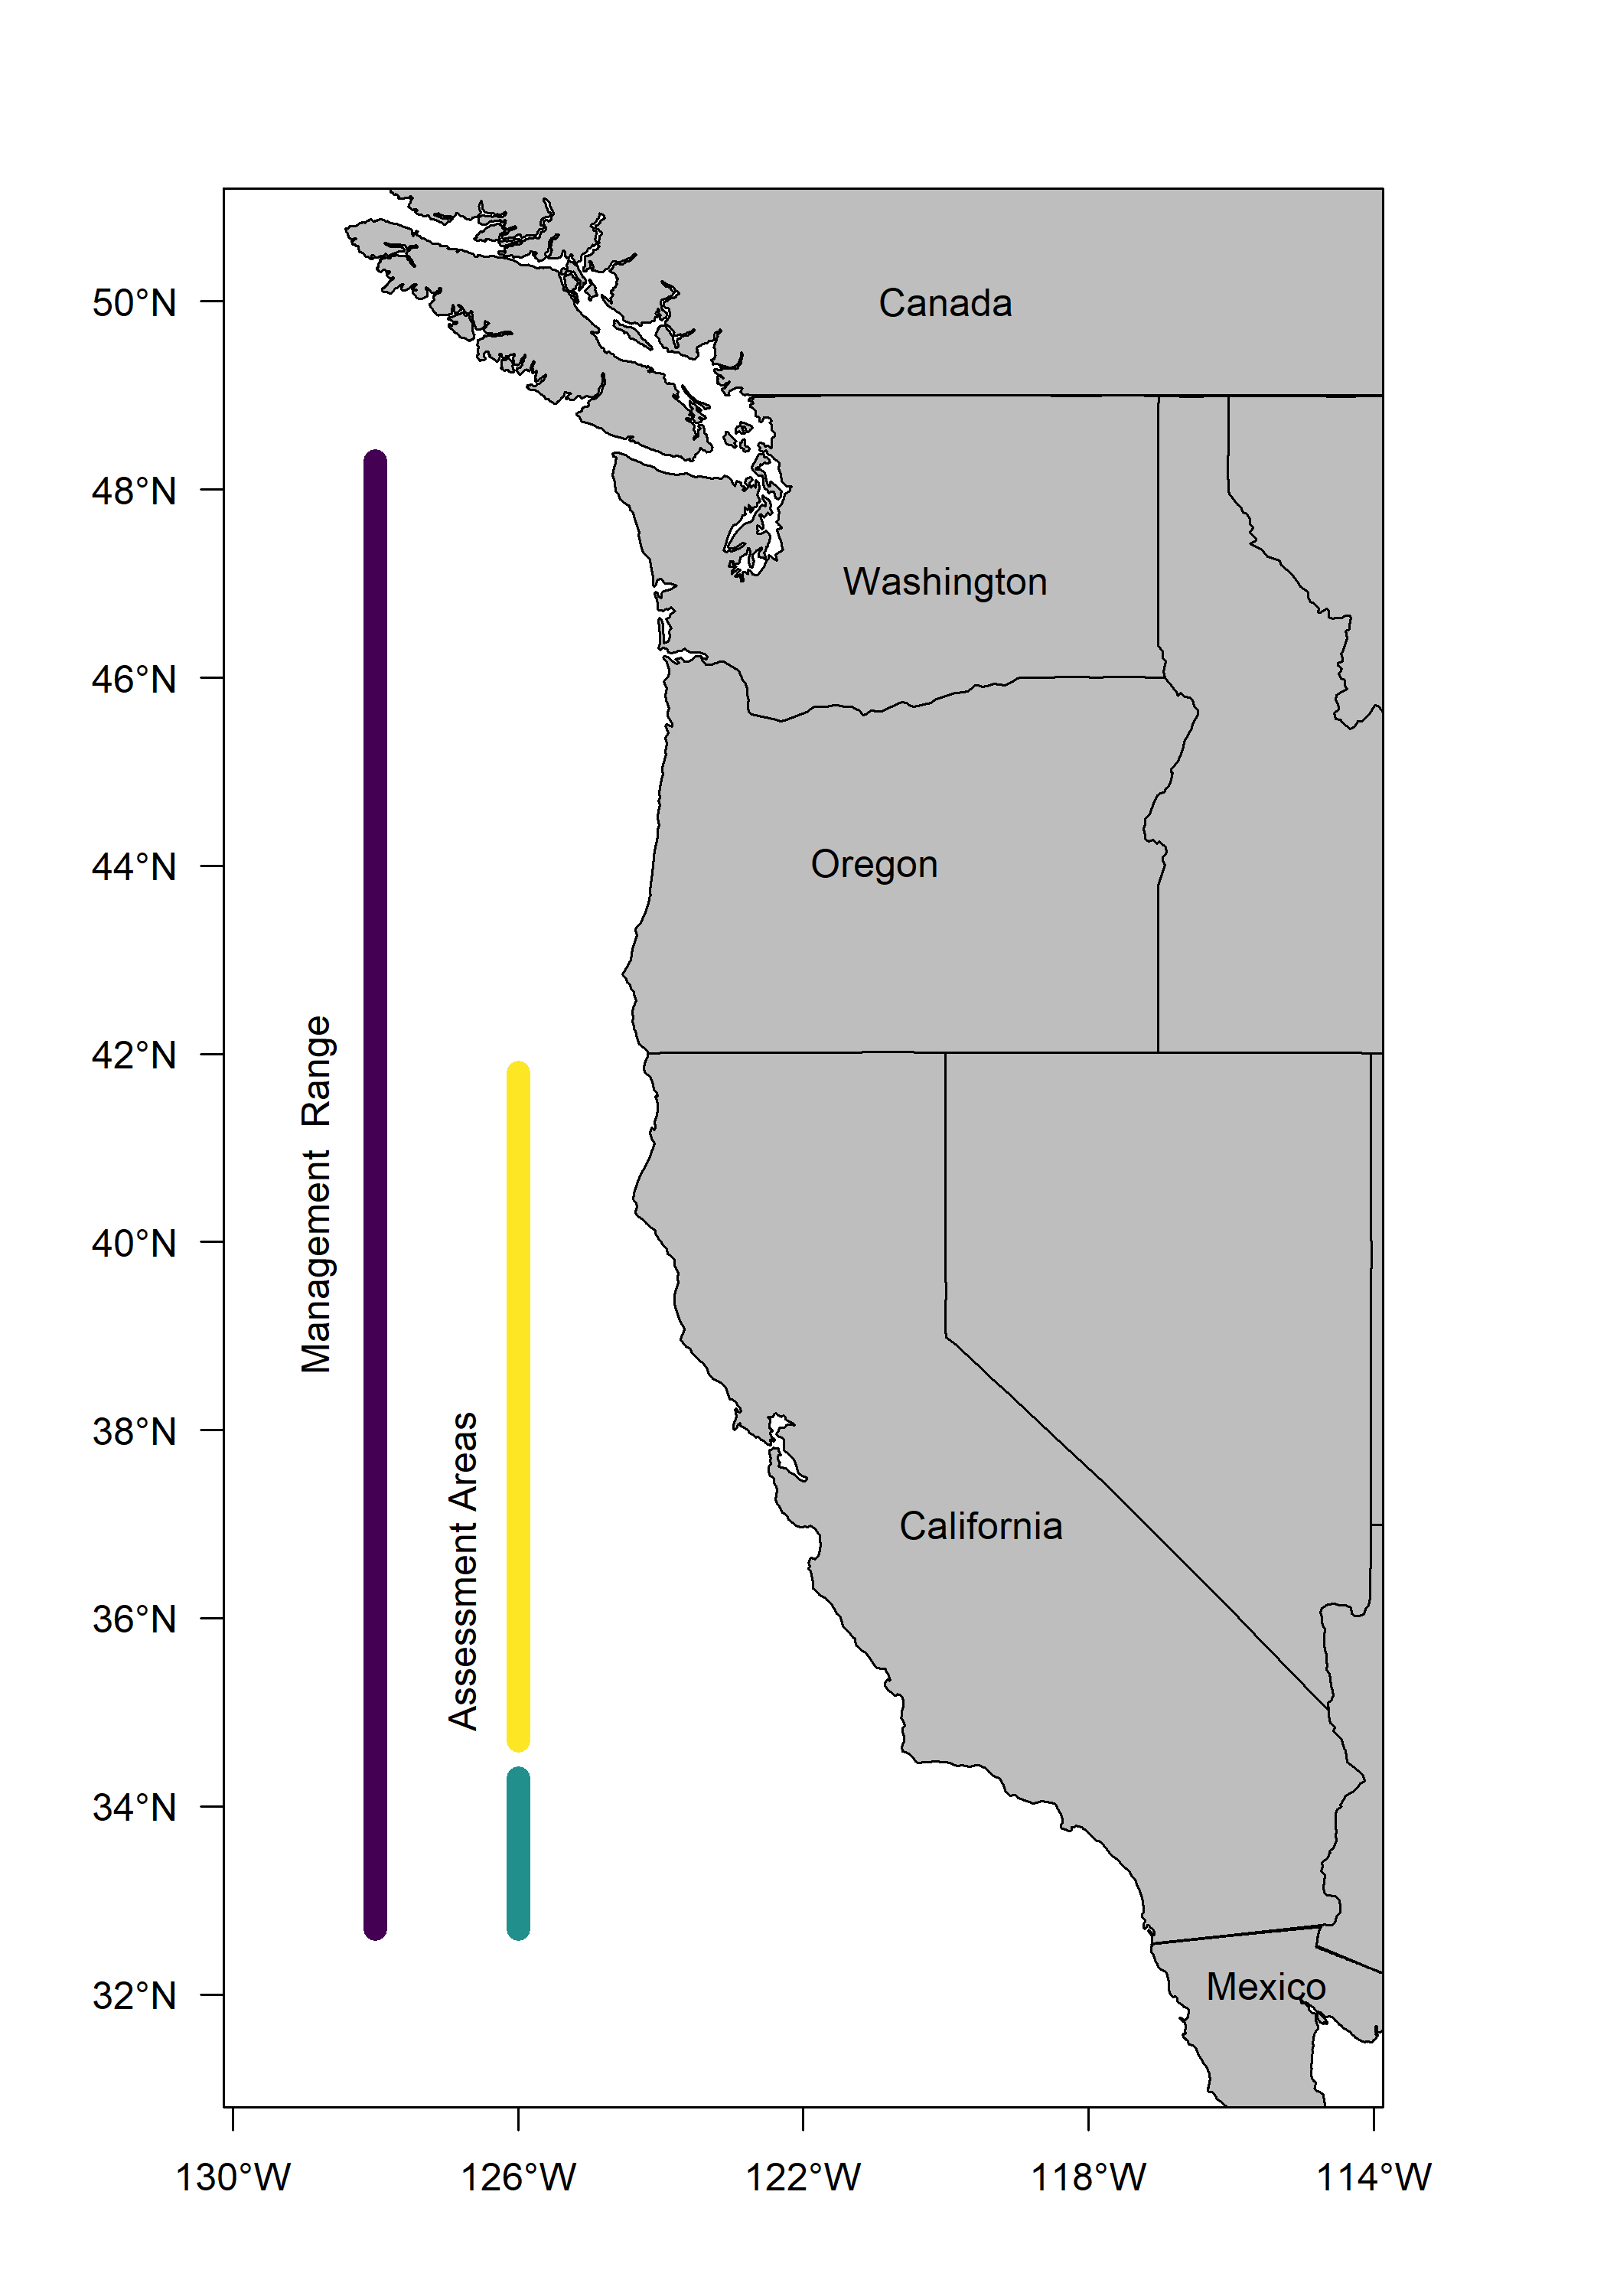
\includegraphics[alt=The management range of copper rockfish off the West Coast covers Washington Oregon and California with the model areas for the California stock modeled south of Point Conception the the U.S. Mexico border and north of Point Conception to the California Oregon border.,width=1\textwidth,height=1\textheight]{C:/Users/melissa.monk/Documents/GitHub/copper_rockfish_2023/documents/shared_figures/map.png}
}
\caption{Map of management area and the 2023 assessment areas for copper rockfish.\label{fig:ca-map}}
\end{figure}

\FloatBarrier

\begin{figure}
{\centering
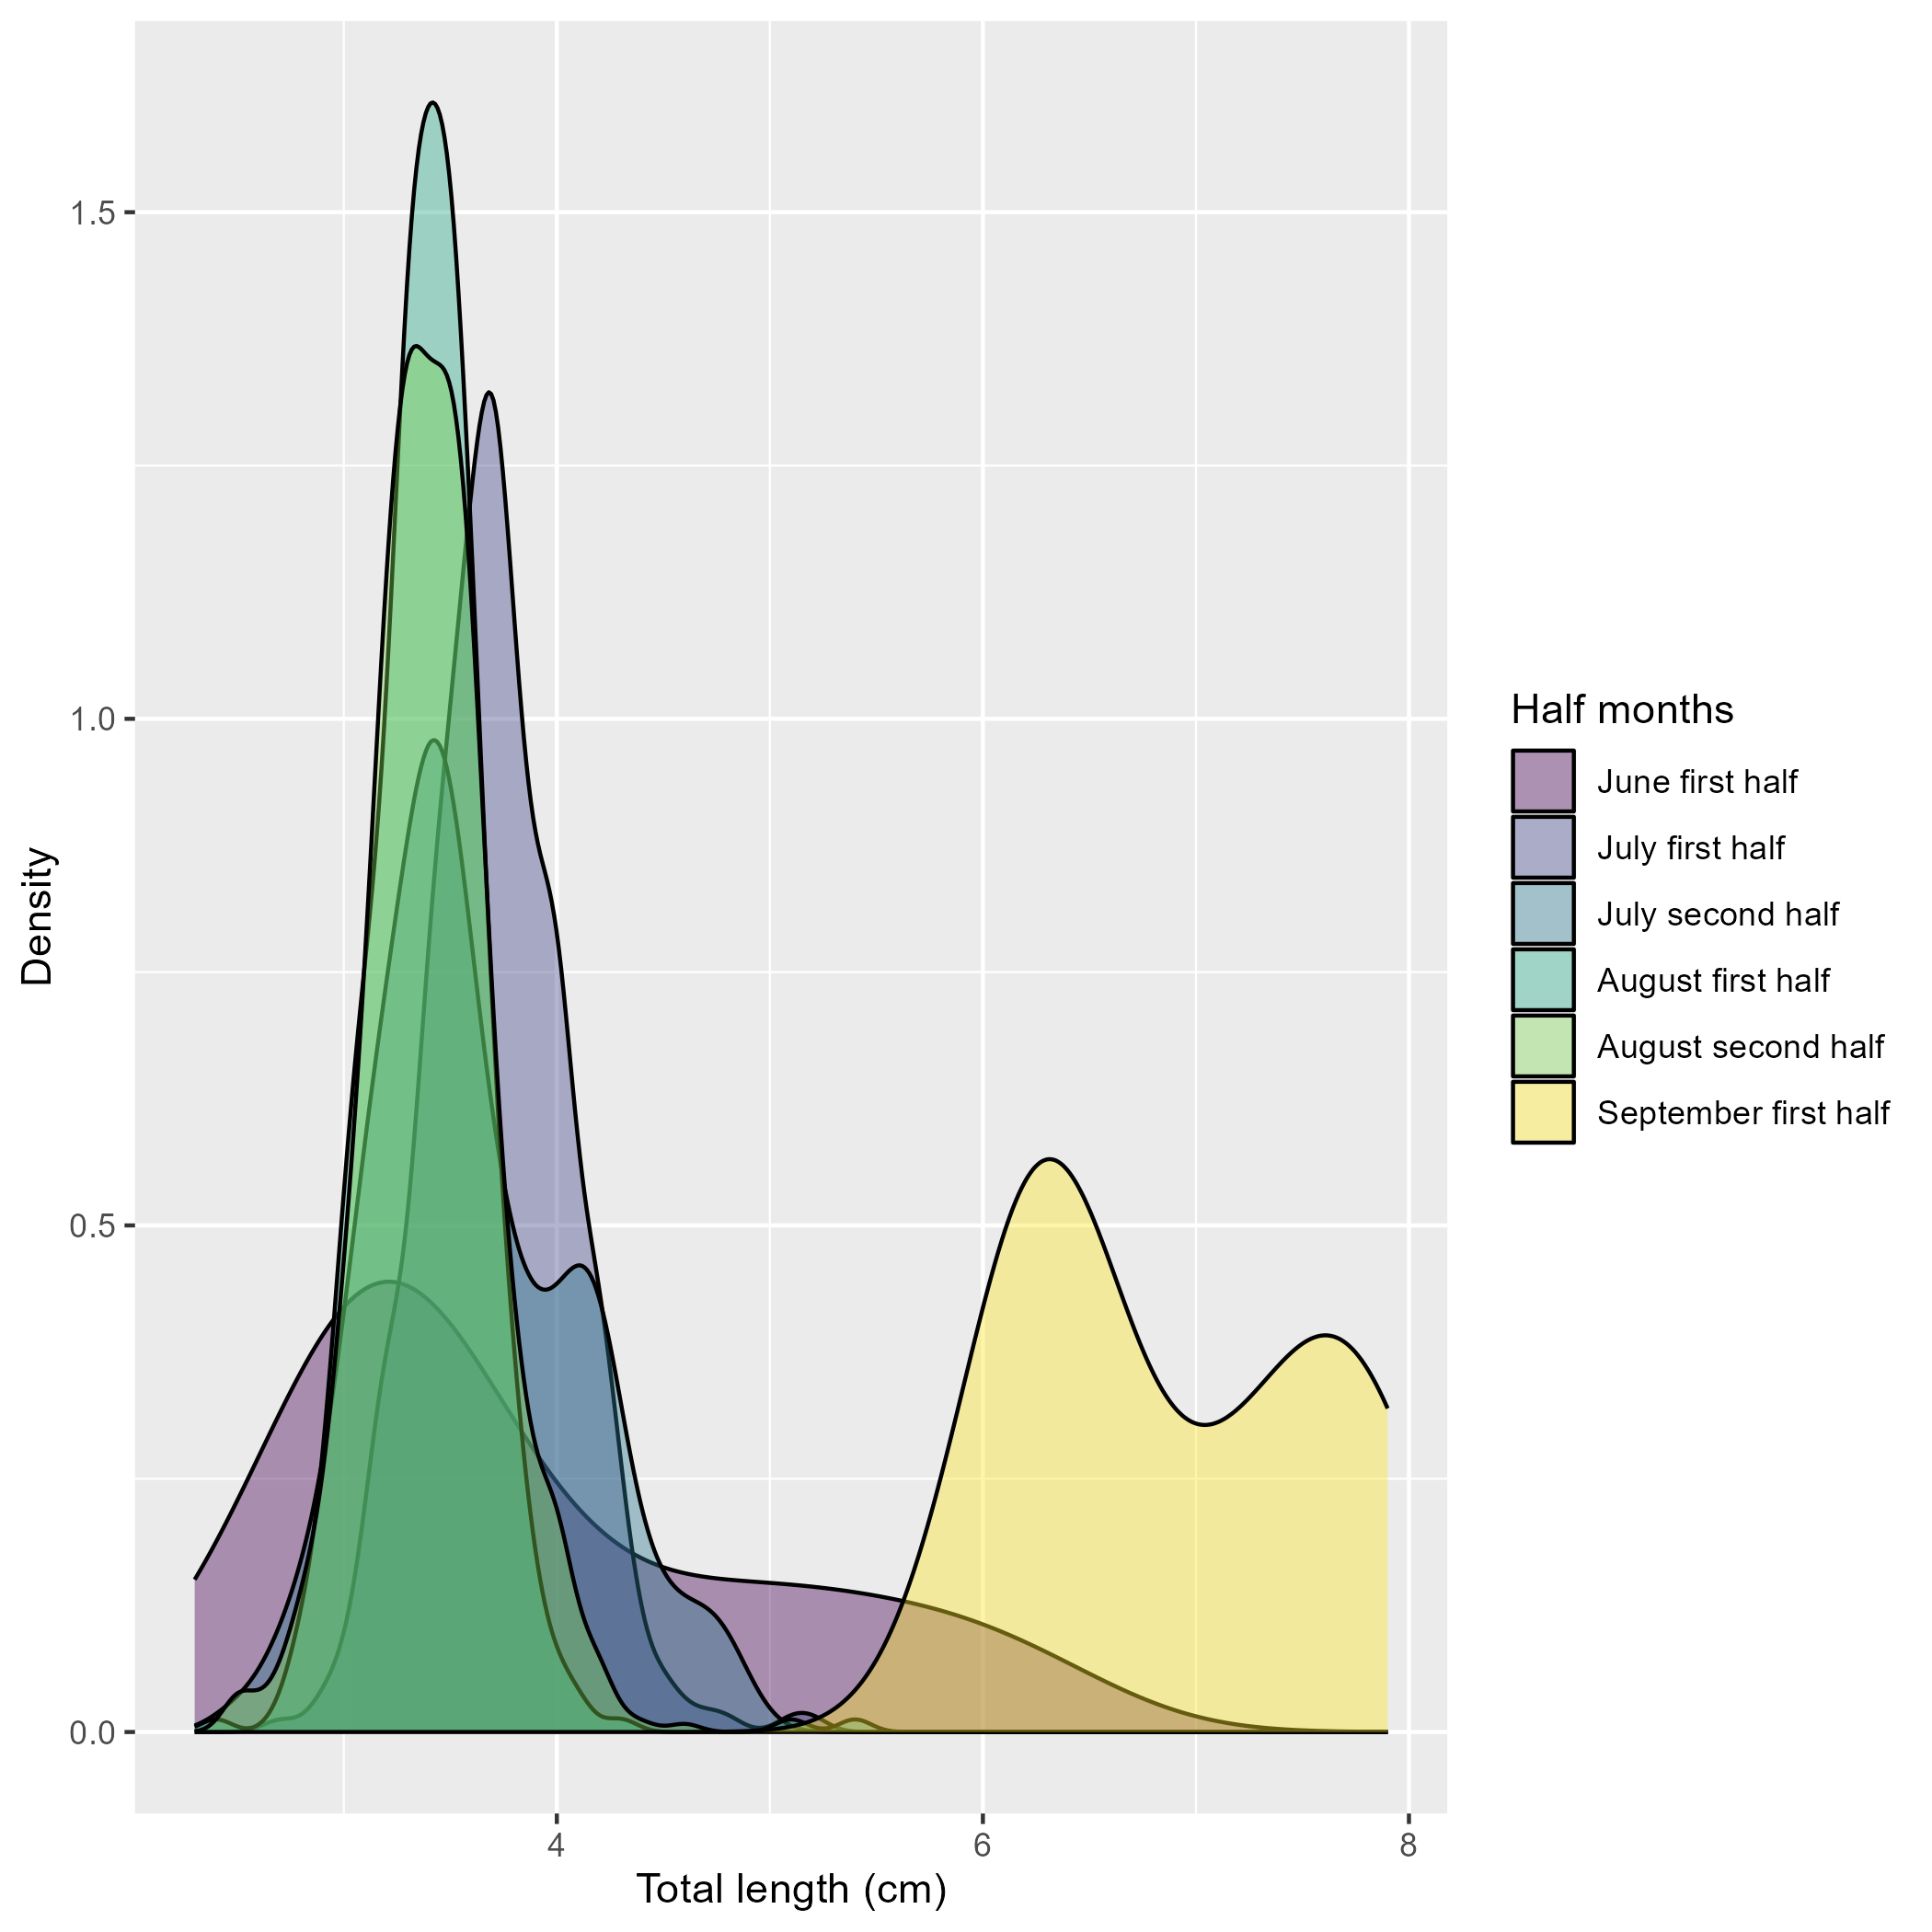
\includegraphics[alt=Observations of young of the year copper rockfish peak between 3 to 4 centimeters between June through August. Observations of young of the year observed in September has a bimodal distribution with sizes peaking between 6 to 7 centimeters and 8 centimeters.,width=1\textwidth,height=1\textheight]{C:/Users/melissa.monk/Documents/GitHub/copper_rockfish_2023/documents/shared_figures/copper_length_by_half_month.png}
}
\caption{Distribution of young-of-the-year copper rockfish lengths from fish genetically identified from D. Baetscher's UCSC dissertation work.\label{fig:copper-smurf-length}}
\end{figure}

\pagebreak

\begin{figure}
{\centering
\includegraphics[alt=Stacked bar plot of landings by fleet used in the base model where catches in metric tons. The landings are below 50 metric tons total until the late 1950s and then increase peaking in the 1970s.  Landing then decline until the early 2000s.  From 2010 to present landings again increase.,width=1\textwidth,height=1\textheight]{S:/copper_rockfish_2023/models/nca/10.0_north_post_star_base/plots/catch2 landings stacked.png}
}
\caption{Landings by fleet used in the base model where catches in metric tons by fleet are stacked.\label{fig:catch}}
\end{figure}

\pagebreak

\begin{figure}
{\centering
\includegraphics[alt=Catch data ar ablor all years modeled from the commercial dead fishery from the mid 1990s for the commercial live fishery and from 1926 to present for the two recreational fleets.  A fishery-independent index from CCFRP was available from 2007 to present. Length composition data were available for all fleets. Marginal ages were available from the recreational charter boat fleet from sparse years in the 1970s and the most recent year.  Conditional age at length data were availble from the commercial dead fishery both recreational fleets CCFRP and various other sources input as a growth fleet.,width=1\textwidth,height=1\textheight]{S:/copper_rockfish_2023/models/nca/10.0_north_post_star_base/plots/data_plot.png}
}
\caption{Summary of data sources used in the base model.\label{fig:data-plot}}
\end{figure}

\FloatBarrier

\begin{figure}
{\centering
\includegraphics[alt=A map of the northern Califonria assessment area with the total number of copper rockfish observed by site for each of the fishery-indpendent surveys considered. Copper rockfish were most commonly observed in shallower waters and over rocky habitat.,width=1\textwidth,height=1\textheight]{S:/copper_rockfish_2023/data/survey_indices/NorthernCA.png}
}
\caption{Map of northern California assessment area with the total number of copper rockfish observed by site for each of the fishery-indpendent surveys considered. Also shown is the network of MPAs, the 3nm state maritime boundary and the CDFW blocks. The CDFW blocks are colored a darker blue   if copper rockfish were observed by a survey and based on expert opinion from the fleet.\label{fig:survey-map}}
\end{figure}

\pagebreak

\begin{figure}
{\centering
\includegraphics[alt=The commercial dead fishery generally catches fish of 25 centimeters or larger.,width=1\textwidth,height=1\textheight]{S:/copper_rockfish_2023/models/nca/10.0_north_post_star_base/plots/comp_lendat_bubflt1mkt0.png}
}
\caption{Length composition data from the commercial dead fleet.\label{fig:com-dead-len-data}}
\end{figure}

\pagebreak

\begin{figure}
{\centering
\includegraphics[alt=Mean length for the commercial dead fleet were availbe from 1979 to 1981 1991 to 2000 2001 and 2016 to 2021. Mean length was around 40 to 45 centimeters for the majority of the time period and decreased to around 30 centimeters startin in 2019.,width=1\textwidth,height=1\textheight]{S:/copper_rockfish_2023/models/nca/10.0_north_post_star_base/plots/comp_lendat_data_weighting_TA1.8_Commercial_Dead.png}
}
\caption{Mean length for commercial dead fleet with 95 percent confidence intervals.\label{fig:mean-com-dead-len-data}}
\end{figure}

\pagebreak

\begin{figure}
{\centering
\includegraphics[alt=The condition age at length composition through time follows the expected patter of the growth curve with the data trunkcated in some yeras to fish 40 centimeters and larger.,width=1\textwidth,height=1\textheight]{S:/copper_rockfish_2023/models/nca/10.0_north_post_star_base/plots/comp_condAALdat_bubflt1mkt0.png}
}
\caption{Conditional age-at-length composition data from the commercial dead fleet.\label{fig:com-dead-age-data}}
\end{figure}

\pagebreak

\begin{figure}
{\centering
\includegraphics[alt=The commercial live fishery generally catches fish between 22 and 50 centimeters.,width=1\textwidth,height=1\textheight]{S:/copper_rockfish_2023/models/nca/10.0_north_post_star_base/plots/comp_lendat_bubflt2mkt0.png}
}
\caption{Length composition data from the commercial live fleet.\label{fig:com-live-len-data}}
\end{figure}

\pagebreak

\begin{figure}
{\centering
\includegraphics[alt=The mean length for the commercial live fishery was between 34 and 45 centimeters until 2011 when it decreased to 27 to approximately 30 centimeters for the remainder of the time series. .,width=1\textwidth,height=1\textheight]{S:/copper_rockfish_2023/models/nca/10.0_north_post_star_base/plots/comp_lendat_data_weighting_TA1.8_Commercial_Live.png}
}
\caption{Mean length for commercial live fleet with 95 percent confidence intervals.\label{fig:mean-com-live-len-data}}
\end{figure}

\pagebreak

\pagebreak

\begin{figure}
{\centering
\includegraphics[alt=The recreational Deb Wilson-Vandenbergy CPFV index remains fairly constant from 1988 to 1992 and then then declines steadily from 1993 to 1998.,width=1\textwidth,height=1\textheight]{S:/copper_rockfish_2023/data/rec_indices/debwv_cpfv_onboard/deltalogn/Index.png}
}
\caption{Estimated annual index of abundances for the CPFV fleet based on the Deb Wilson-Vandenberg survey data.\label{fig:dwv-index-main}}
\end{figure}

\pagebreak

\begin{figure}
{\centering
\includegraphics[alt=The recreational CPFV index increases from 1999 to 2001 decreases slightly and remains constant for three years.  The index from 2005 to 2008 is steady at the level observed in 2001 and then decreases in 2008.  The index generally increases from 2009 to 2021.,width=1\textwidth,height=1\textheight]{S:/copper_rockfish_2023/data/rec_indices/crfs_cpfv_onboard/north/area_weighted/Index.png}
}
\caption{Estimated annual index of abundances for the CPFV fleet based on CRFS survey data.\label{fig:crfs-index-main}}
\end{figure}

\pagebreak

\begin{figure}
{\centering
\includegraphics[alt=The private/rental mode index of abundance remains flat and uniformative from 2004 to 2014.  The index increaes in 2015 spikess to a high relative value from 20 to 50 in 2017.  The last two years of the index are higher than 2015 but lower than the value in 2017.,width=1\textwidth,height=1\textheight]{S:/copper_rockfish_2023/data/rec_indices/crfs_pr_dockside/north/rm_last2yrs_area_weighted/Index.png}
}
\caption{Estimated annual index of abundances for the private/rental fleet based on CRFS survey data.\label{fig:crfs-pr-index-main}}
\end{figure}

\pagebreak

\begin{figure}
{\centering
\includegraphics[alt=The recreational fleet generally catches fish between 22 and 50 centimeters.,width=1\textwidth,height=1\textheight]{S:/copper_rockfish_2023/models/nca/10.0_north_post_star_base/plots/comp_lendat_bubflt3mkt0_page2.png}
}
\caption{Length composition data from the recreational CPFV fleet.\label{fig:rec-cpfv-len-data}}
\end{figure}

\pagebreak

\begin{figure}
{\centering
\includegraphics[alt=The mean length from the recreational CPFV fleet is uncertain until 1980 at which point it ranges from 35 to 40 centimeters for the remainder of the time series.,width=1\textwidth,height=1\textheight]{S:/copper_rockfish_2023/models/nca/10.0_north_post_star_base/plots/comp_lendat_data_weighting_TA1.8_Rec_CPFV.png}
}
\caption{Mean length for recreational CPFV fleet with 95 percent confidence intervals.\label{fig:mean-rec-cpfv-len-data}}
\end{figure}

\pagebreak

\begin{figure}
{\centering
\includegraphics[alt=The recreational private rental fleet catches fish range from 20 to 50 centimeters with the after fish around 30 centimeters.,width=1\textwidth,height=1\textheight]{S:/copper_rockfish_2023/models/nca/10.0_north_post_star_base/plots/comp_lendat_flt4mkt0_page2.png}
}
\caption{Length composition data from the recreational PR fleet.\label{fig:rec-pr-len-data}}
\end{figure}

\pagebreak

\begin{figure}
{\centering
\includegraphics[alt=The mean length in the private rental fleet is more uncertain then tha charter fleet until 2003. The average length ranges from 35 to 40 centimeters from 1978 to 1985.  The average length then remains around 30 to 35 centimeters for the remainders of the time series.,width=1\textwidth,height=1\textheight]{S:/copper_rockfish_2023/models/nca/10.0_north_post_star_base/plots/comp_lendat_data_weighting_TA1.8_Rec_PR.png}
}
\caption{Mean length for recreational PR fleet with 95 percent confidence intervals.\label{fig:mean-rec-pr-len-data}}
\end{figure}

\FloatBarrier

\begin{figure}
{\centering
\includegraphics[alt=The majority of the fish aged from the recreational CPFV fleet were less than 15 years old.,width=1\textwidth,height=1\textheight]{S:/copper_rockfish_2023/models/nca/10.0_north_post_star_base/plots/comp_condAALdat_bubflt3mkt0.png}
}
\caption{Conditional age-at-length composition data from the recreational CPFV fleet.\label{fig:rec-cpfv-caal-data}}
\end{figure}

\pagebreak

\begin{figure}
{\centering
\includegraphics[alt=There are sparse age data for the recreational CPFV fleet. The average age from 1978 to 1985 is 10 to 15 years and in 2021 is around 10 years old.,width=1\textwidth,height=1\textheight]{S:/copper_rockfish_2023/models/nca/10.0_north_post_star_base/plots/comp_agedat_data_weighting_TA1.8_Rec_CPFV.png}
}
\caption{Mean age for recreational CPFV fleet with 95 percent confidence intervals.\label{fig:mean-rec-cpfv-age-data}}
\end{figure}

\FloatBarrier

\begin{figure}
{\centering
\includegraphics[alt=The marginal age compositions suggest the majority of fish caught by the CPFV fleet are less than 20 years old. .,width=1\textwidth,height=1\textheight]{S:/copper_rockfish_2023/models/nca/10.0_north_post_star_base/plots/comp_agedat__aggregated_across_time.png}
}
\caption{Marginal age composition data aggregate across the 1978, 1981, 1984, and 2022 (carcass ages) data years from the CPFV fleet.\label{fig:rec-cpfv-marg-age-data}}
\end{figure}

\pagebreak

\begin{figure}
{\centering
\includegraphics[alt=Comparison of all length collected by the CRFS sampling program for the CPFV fleet to the lengths from the fish with ages from the cooperative sampling program. The length distributions in the area north of Point Conception are in general agreement while the distribution of lengths collected by this program does not align with the length samples from CRFS.,width=1\textwidth,height=1\textheight]{S:/copper_rockfish_2023/data/ages/plots/coop_crfs_length_comparison.png}
}
\caption{Comparison of all length collected by the CRFS sampling program for the CPFV fleet to the lengths from the fish with ages from the cooperative sampling program. The length distributions in the area north of Point Conception are in general agreement while the distribution of lengths collected by this program does not align with the length samples from CRFS.\label{fig:coop-len-comparison}}
\end{figure}

\pagebreak

\begin{figure}
{\centering
\includegraphics[alt=The conditional age at length compositions suggest the majority of fish caught by the CPFV fleet are less than 20 years old.,width=1\textwidth,height=1\textheight]{S:/copper_rockfish_2023/models/nca/10.0_north_post_star_base/plots/comp_condAALdat_bubflt4mkt0.png}
}
\caption{Conditional age-at-length data for recreational PR collected in 2022.\label{fig:rec-pr-caal-data}}
\end{figure}

\pagebreak

\begin{figure}
{\centering
\includegraphics[alt=A map of the nortern California assessment area showing locations sampled by the fishery-indpendent surveys and the MPAs.,width=1\textwidth,height=1\textheight]{S:/copper_rockfish_2023/data/survey_indices/plots/north_survey_locations_designation.png}
}
\caption{Sample locations by each of the fishery-independent data sources used in the base model with indices of abundance, lengths, and ages if collected.\label{fig:survey-locations}}
\end{figure}

\pagebreak

\begin{figure}
{\centering
\includegraphics[alt=Sample locations from the CCFRP and CDFW ROV surveys inside and adjacent to MPAs in northern California.,width=1\textwidth,height=1\textheight]{S:/copper_rockfish_2023/data/survey_indices/plots/north_survey_locations.png}
}
\caption{Sample locations by area areas open to fishing (reference) and MPAS for each of the fishery-independent data sources used in the base model with indices of abundance, lengths, and ages if collected.\label{fig:ref-mpa}}
\end{figure}

\pagebreak

\begin{figure}
{\centering
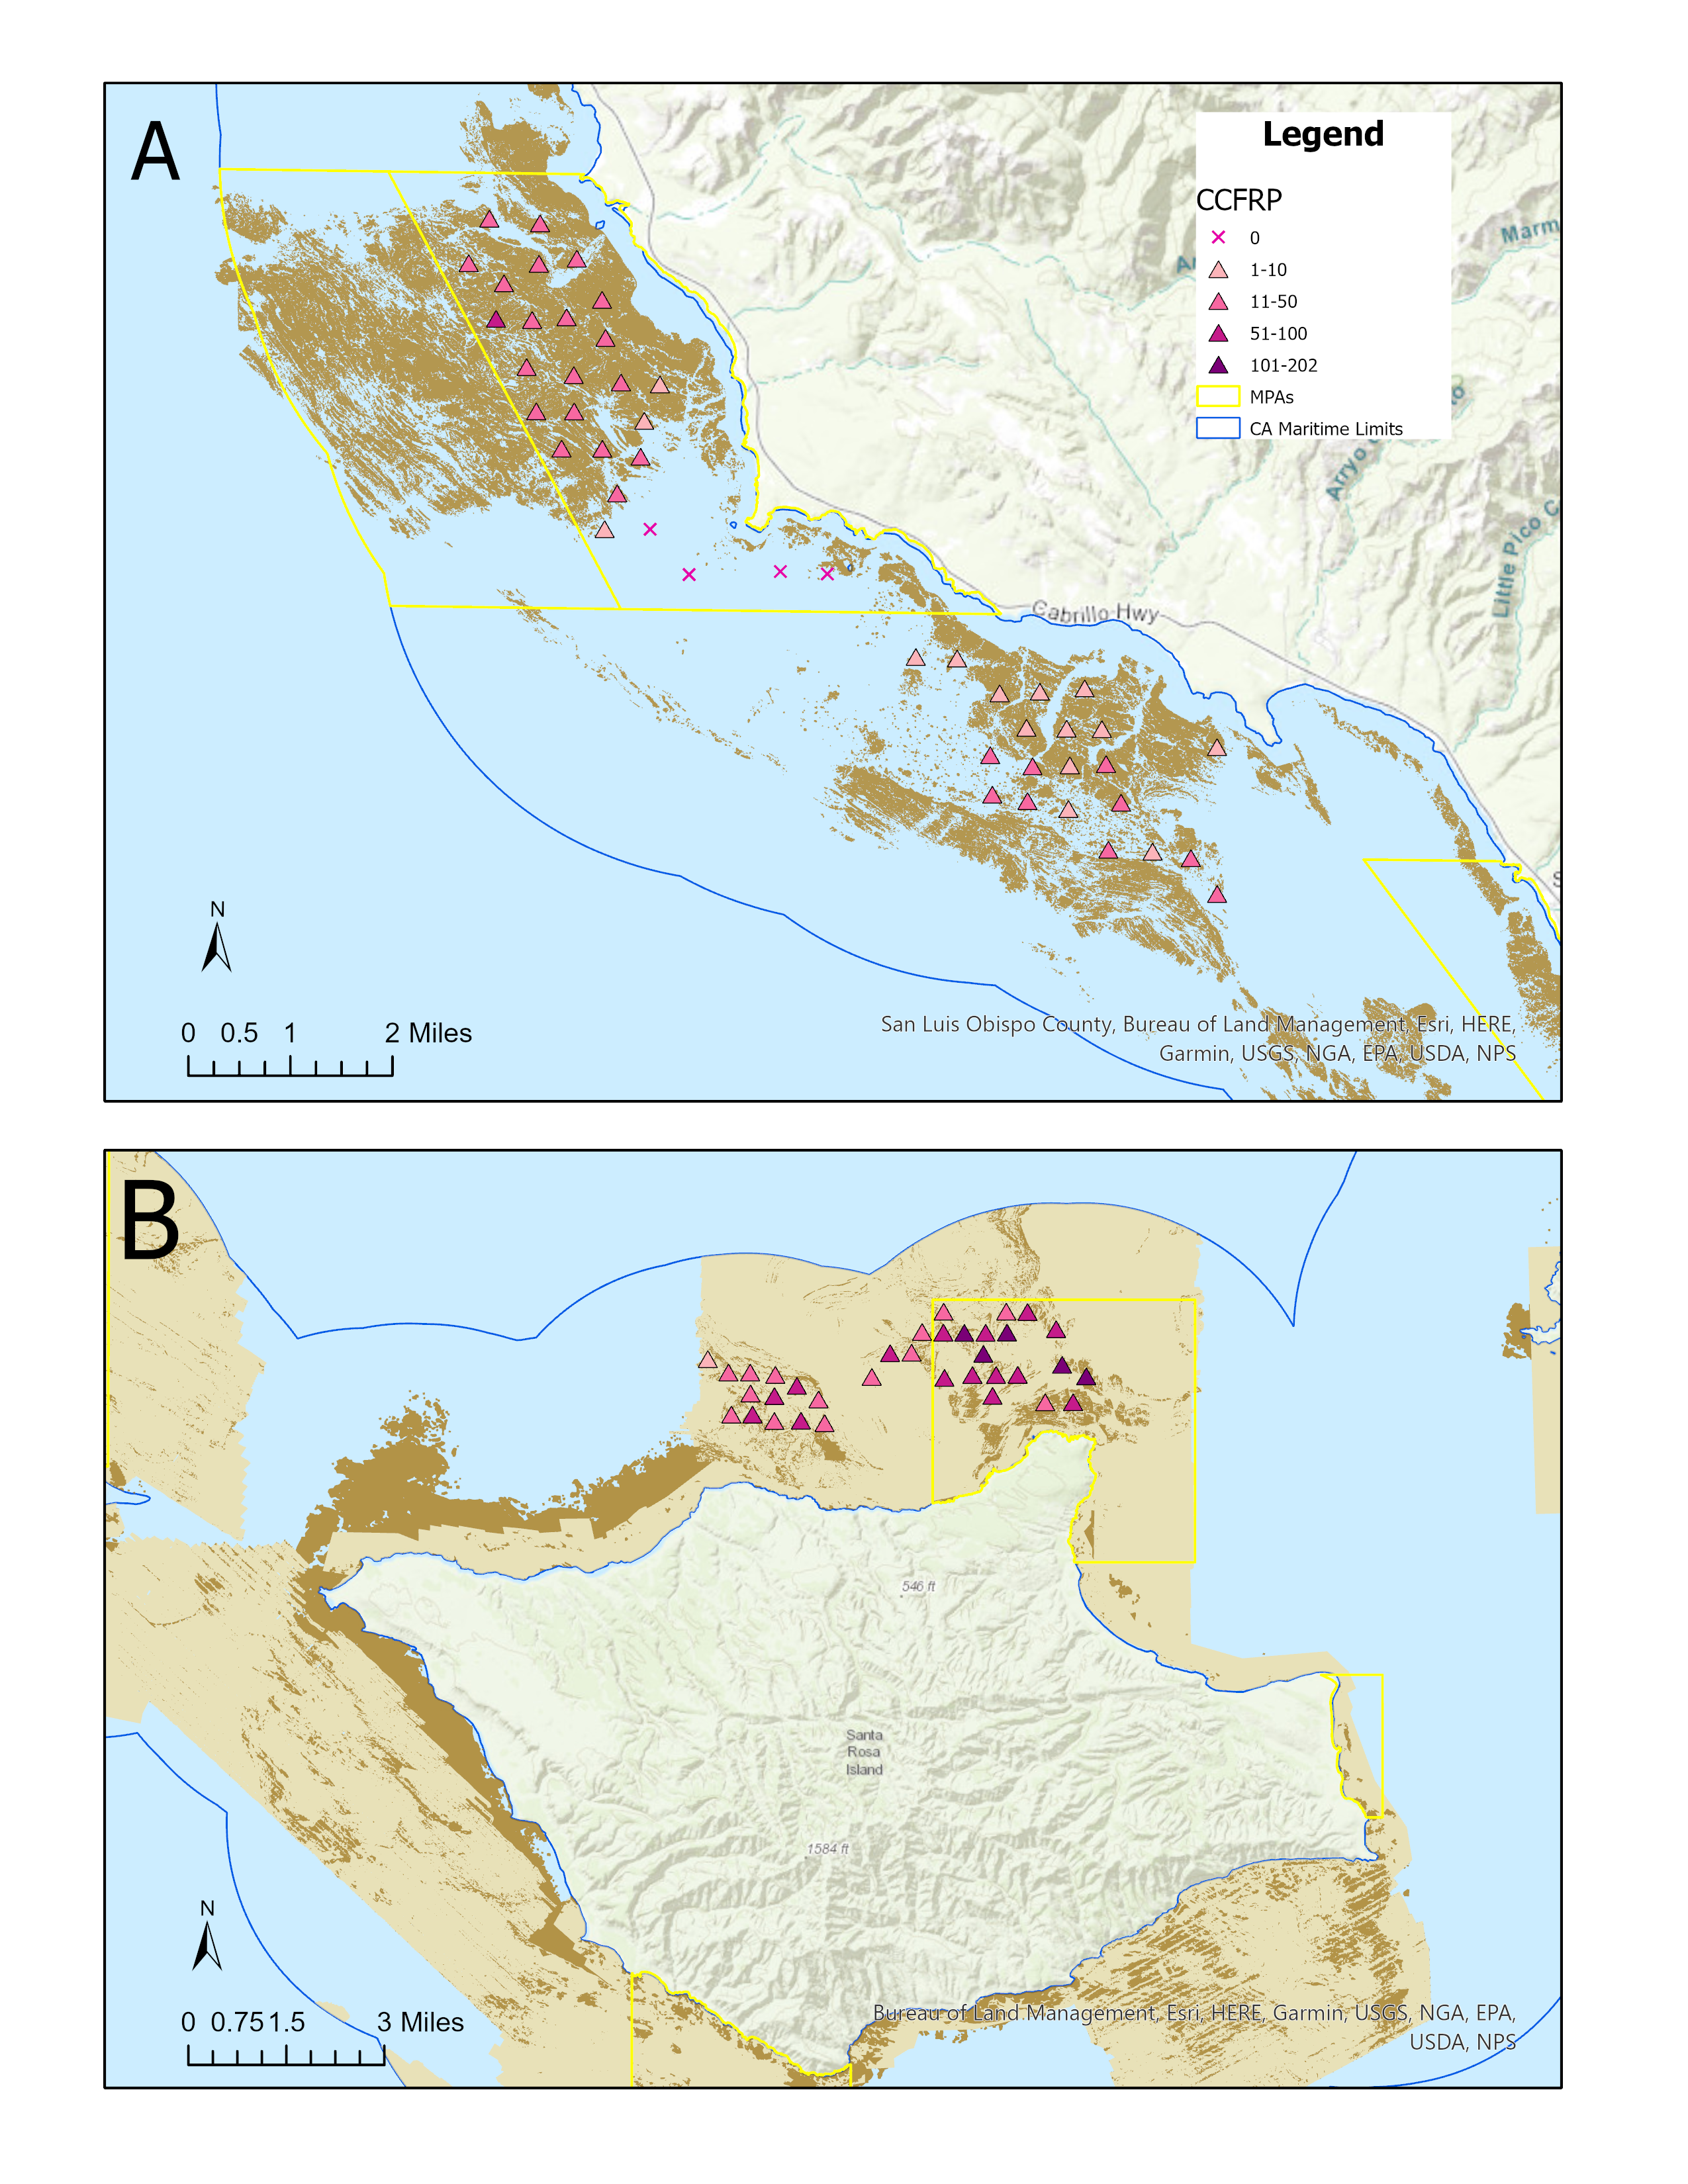
\includegraphics[alt=Map depicting copper rockfish observations from the Piedras Blancas MPA and reference sites for CCFRP in northern California A and the Carrington Point MPA and reference sites in southern California. The examples from each area show the differences in the available interpreted rocky substrate. Rocky habitat (in brown) is depicted for northern California and the areas that have been interpreted for the area shown in southern California are in tan with the rocky substrate in brown.  The lower resolution rocky substrate (outside the tan areas) depicted in southern California represents interpreted substrate from courser bathymetry data.,width=1\textwidth,height=1\textheight]{C:/Users/melissa.monk/Documents/GitHub/copper_rockfish_2023/documents/shared_figures/ccfrp_map.png}
}
\caption{Map depicting copper rockfish observations from the Piedras Blancas MPA and reference sites for CCFRP in northern California (A) and the Carrington Point MPA and reference sites in southern California. The examples from each area show the differences in the available interpreted rocky substrate. Rocky habitat (in brown) is depicted for northern California and the areas that have been interpreted for the area shown in southern California are in tan with the rocky substrate in brown.  The lower resolution rocky substrate (outside the tan areas) depicted in southern California represents interpreted substrate from courser bathymetry data. .\label{fig:ccfrp-map}}
\end{figure}

\begin{figure}
{\centering
\includegraphics[alt=The relative index for CCFRP is flat from 2007 to 2015 and steadily increases for the remainder of the time series.,width=1\textwidth,height=1\textheight]{S:/copper_rockfish_2023/data/survey_indices/ccfrp/north/area_weighted/Index.png}
}
\caption{Estimated relative index of abundance from the CCFRP Hook and Line survey.\label{fig:ccfrp-index-main}}
\end{figure}

\pagebreak

\begin{figure}
{\centering
\includegraphics[alt=CCFRP generally catches fish ranging from 20 to 50 centimeters. .,width=1\textwidth,height=1\textheight]{S:/copper_rockfish_2023/models/nca/10.0_north_post_star_base/plots/comp_lendat_bubflt5mkt0.png}
}
\caption{Length composition data from the CCFRP Hook and Line survey.\label{fig:ccfrp-len-data}}
\end{figure}

\pagebreak

\begin{figure}
{\centering
\includegraphics[alt=The mean length of fish caught by CCFRP range increases from 34 cm in 2007 to 38 centimeters in 2022.,width=1\textwidth,height=1\textheight]{S:/copper_rockfish_2023/models/nca/10.0_north_post_star_base/plots/comp_lendat_data_weighting_TA1.8_CCFRP.png}
}
\caption{Mean length for the CCFRP Hook and Line survey with 95 percent confidence intervals.\label{fig:ccfrp-mean-len-data}}
\end{figure}

\pagebreak

\begin{figure}
{\centering
\includegraphics[alt=The range of age at length of fish caught by CCFRp are younger than approximatley 10 years of age from 2018 to 2019 and in 2022 observed fihs older than 10.,width=1\textwidth,height=1\textheight]{S:/copper_rockfish_2023/models/nca/10.0_north_post_star_base/plots/comp_condAALdat_bubflt5mkt0.png}
}
\caption{Conditional age-at-length data from the CCFRP Hook and Line survey.\label{fig:ccfrp-age-data}}
\end{figure}

\pagebreak

\pagebreak

\pagebreak

\pagebreak

\pagebreak

\pagebreak

\pagebreak

\begin{figure}
{\centering
\includegraphics[alt=The peak of the distirbution for the cooperative CPFV and Peasron lengths peaked around 35 centimeters and the WCGBT survey length distribution peaks around 45 centimeters.,width=1\textwidth,height=1\textheight]{S:/copper_rockfish_2023/data/ages/plots/south_growth_length_comparison.png}
}
\caption{Length distribution of fish by collection source that were used as conditional age-at-length data in the growth fleet.\label{fig:growth-len-dist}}
\end{figure}

\pagebreak

\begin{figure}
{\centering
\includegraphics[alt=The peasek of the distirbutions of ages for the cooperative CPFV and Pearson collections were around 10 years and the WCGBT survey age distribution peaked at around 6 years of age.,width=1\textwidth,height=1\textheight]{S:/copper_rockfish_2023/data/ages/plots/south_growth_age_comparison.png}
}
\caption{Age distribution of fish by collection source that were used as conditional age-at-length data in the growth fleet.\label{fig:growth-age-dist}}
\end{figure}

\pagebreak

\begin{figure}
{\centering
\includegraphics[alt=Locations of copper rockfish from visual surveys along the coast that were not included in the stock assessment.,width=1\textwidth,height=1\textheight]{C:/Users/melissa.monk/Documents/GitHub/copper_rockfish_2023/documents/shared_figures/visual_surveys.png}
}
\caption{Locations copper rockfish were observed from visual surveys from Milton Love's submersible survey of natural reefs and oil platforms (RIGS) and additional visual surveys conducted by the SWFSC.\label{fig:visual-surveys}}
\end{figure}

\begin{figure}
{\centering
\includegraphics[alt=Indices of abundance that show improbable estimates of CPUE among counties and indicate a noisy dataset from the MRFSS period of sampling.,width=1\textwidth,height=1\textheight]{S:/copper_rockfish_2023/data/rec_indices/mrfss_cpfv_dockside/north/plots/average_cpue_by_cnty.png}
}
\caption{Average CPUE by county from the MRFSS dockside data north of Point Conception. Note the break in years from 1989-1995.\label{fig:mrfss-cpue-county}}
\end{figure}

\begin{figure}
{\centering
\includegraphics[alt=Bubble plot showing the uncommmonly encountered copper rockfish fromt he WCGBT survey.  Most copper rockfish observered were near Monterey Bay and and Morro Bay.,width=1\textwidth,height=1\textheight]{S:/copper_rockfish_2023/data/wcgbt/north/plots/cpue_map.png}
}
\caption{Location and catch-per-unit-effort by location caught north of Point Conception by the NWFSC WCGBT survey.\label{fig:wcgbt-cpue}}
\end{figure}

\pagebreak

\begin{figure}
{\centering
\includegraphics[alt=Very few copper rockfish were observed in the WCGBTS.  The majority of coppers were observed between 50 and 100 meters depth.,width=1\textwidth,height=1\textheight]{S:/copper_rockfish_2023/data/wcgbt/north/plots/presence-absence_proportion_by_depth.png}
}
\caption{Proportion of positive tows across all years by depth in meters from the NWFSC WCGBT survey.\label{fig:wcgbt-depth}}
\end{figure}

\pagebreak

\begin{figure}
{\centering
\includegraphics[alt=The WCGBT survey provided age data for the assessment.  No clear trend of differences in growth rates between males and females were observed in the plot of the available age at length data. Some of the smallest fish observed had undetermined sex.,width=1\textwidth,height=1\textheight]{S:/copper_rockfish_2023/data/wcgbt/plots/wcgbt_north_age_at_length_by_area.png}
}
\caption{Age and length by sex for copper rockfish caught north of Point Conception by the NWFSC WCGBT survey.\label{fig:wcgbt-len-age}}
\end{figure}

\pagebreak

\subsection{Biology}\label{biology}

\begin{figure}
{\centering
\includegraphics[alt=The highest frequency of older aged fish peaking between 5-15 years were observed in California north of Point Conception. Souths of Point Conception in California the the highest frequency of ages peaking around 6 years of age. The highest frequency of ages in both Oregon and Washington peaked around 8 years of age.,width=1\textwidth,height=1\textheight]{S:/copper_rockfish_2023/data/ages/plots/west_coast_age_density.png}
}
\caption{Densities of aged copper rockfish by U.S. West Coast areas and limited samples from the Gulf of Alaska (25 fish).\label{fig:west-coast-age-density}}
\end{figure}

\pagebreak

\begin{figure}
{\centering
\includegraphics[alt=Logistic maturity curve with fish starting to become mature at 25 cenitmeters and full maturity by 43 centimeters.,width=1\textwidth,height=1\textheight]{S:/copper_rockfish_2023/models/nca/10.0_north_post_star_base/plots/bio6_maturity.png}
}
\caption{Maturity as a function of length.\label{fig:maturity}}
\end{figure}

\pagebreak

\begin{figure}
{\centering
\includegraphics[alt=Exponential curve of fecundity by length with the largest length fish having the highest fecundity.,width=1\textwidth,height=1\textheight]{S:/copper_rockfish_2023/models/nca/10.0_north_post_star_base/plots/bio9_fecundity_len.png}
}
\caption{Fecundity as a function of length.\label{fig:fecundity}}
\end{figure}

\pagebreak

\begin{figure}
{\centering
\includegraphics[alt=Proportion of fish by sex in two centimeter length bins.  The smallest fish below 10 centimeters had undetermined sex.  The largest average proportion is approximately 50 50 from 18 to 48 centeimeters.  The proportion of sexed fish larger than 52 females is skewed towards female in this dataset.,width=1\textwidth,height=1\textheight]{S:/copper_rockfish_2023/data/wcgbt/plots/length_fraction_female.png}
}
\caption{Fraction of each sex by length by the NWFSC WCGBT survey.\label{fig:frac-sex-len}}
\end{figure}

\pagebreak

\begin{figure}
{\centering
\includegraphics[alt=Fish weight increases with increasing fish length.  There is no difference in the weight to length relationship for males and females.,width=1\textwidth,height=1\textheight]{S:/copper_rockfish_2023/data/biology/plots/Length_Weight_All.png}
}
\caption{Estimated weight-at-length using data from the NWFSC Hook and Line and WCGBT survey.\label{fig:weight-length}}
\end{figure}

\pagebreak

\begin{figure}
{\centering
\includegraphics[alt=Ageing error increases linearly with age.,width=1\textwidth,height=1\textheight]{S:/copper_rockfish_2023/data/ages/ageing_error/B0_S3/Reader_1_vs_Reader_2.png}
}
\caption{Distribution of double reads between age reader 1 and 2.\label{fig:age-error-dist}}
\end{figure}

\pagebreak

\begin{figure}
{\centering
\includegraphics[alt=Linear increase in the ageing imprecision standard deviation.,width=1\textwidth,height=1\textheight]{S:/copper_rockfish_2023/models/nca/10.0_north_post_star_base/plots/numbers5_ageerrorSD.png}
}
\caption{Ageing imprecision standard deviation of observed age in years.\label{fig:age-error}}
\end{figure}

\pagebreak

\begin{figure}
{\centering
\includegraphics[alt=Ageing error increases linear with age.,width=1\textwidth,height=1\textheight]{S:/copper_rockfish_2023/models/nca/10.0_north_post_star_base/plots/numbers10_ageerror_matrix_1.png}
}
\caption{Distribution of observed age at true age for ageing error type 1.\label{fig:age-error-matrix}}
\end{figure}

\pagebreak

\subsection{Model Results}\label{model-results}

\subsubsection{Model Bridging}\label{model-bridging}

\begin{figure}
{\centering
\includegraphics[alt=The stock synthesis models produced the same values of spwaning output.,width=1\textwidth,height=1\textheight]{S:/copper_rockfish_2023/models/nca/_bridging/_plots/0_model_convert_compare2_spawnbio_uncertainty.png}
}
\caption{Stock synthesis model version bridge comparison of estimated spawning output.\label{fig:bridge-ssb}}
\end{figure}

\pagebreak

\begin{figure}
{\centering
\includegraphics[alt=The stock synthesis models produced the same values of estimated fraction of unfished and uncertainty.,width=1\textwidth,height=1\textheight]{S:/copper_rockfish_2023/models/nca/_bridging/_plots/0_model_convert_compare4_Bratio_uncertainty.png}
}
\caption{Model version bridge comparison of estimated fraction unfished.\label{fig:bridge-depl}}
\end{figure}

\pagebreak

\begin{figure}
{\centering
\includegraphics[alt=Additions and updates of data including fleet structure biology removals lengths and ages and fishery indices did not result in large overall changes in the model.  Addition of fishery lengths and ages and indices estimated a higher spawning output in the last three years of the model.,width=1\textwidth,height=1\textheight]{S:/copper_rockfish_2023/models/nca/_bridging/_plots/full_bridge_1_compare2_spawnbio_uncertainty.png}
}
\caption{Model structure and data bridging comparison of estimated spawning output.\label{fig:data-bridge-ssb-1}}
\end{figure}

\pagebreak

\begin{figure}
{\centering
\includegraphics[alt=Additions and updates of data including fleet structure biology removals lengths and ages and fishery indices did not result in large overall changes in the model.  Addition of fishery lengths and ages and indices estimated a higher fraction of unfished in the last three years of the model.,width=1\textwidth,height=1\textheight]{S:/copper_rockfish_2023/models/nca/_bridging/_plots/full_bridge_1_compare4_Bratio_uncertainty.png}
}
\caption{Model structure and data bridging comparison of estimated fraction unfished.\label{fig:data-bridge-depl-1}}
\end{figure}

\pagebreak

\begin{figure}
{\centering
\includegraphics[alt=.,width=1\textwidth,height=1\textheight]{S:/copper_rockfish_2023/models/nca/_bridging/_plots/full_bridge_2_compare2_spawnbio_uncertainty.png}
}
\caption{Model structure and data bridging comparison of estimated spawning output.\label{fig:data-bridge-ssb-2}}
\end{figure}

\pagebreak

\begin{figure}
{\centering
\includegraphics[alt=Addition of the ROV indices and lengths and the fishery independent data ressulted in higher estimates of sapwning output in the ending years of the model.,width=1\textwidth,height=1\textheight]{S:/copper_rockfish_2023/models/nca/_bridging/_plots/full_bridge_2_compare4_Bratio_uncertainty.png}
}
\caption{Model structure and data bridging comparison of estimated fraction unfished.\label{fig:data-bridge-depl-2}}
\end{figure}

\pagebreak

\begin{figure}
{\centering
\includegraphics[alt=The caption contains a detailed description of fishing regulations.,width=1\textwidth,height=1\textheight]{S:/copper_rockfish_2023/management/fishing_regs.png}
}
\caption{The CDFW recreational season length and depth restriction for nearshore rockfish by month from 2000 to 2003. A triangle indicates a regulation change mid-month. The regions defined base on the following latitudes: Northern ($42^\circ 00^\prime$ N. lat. to $40^\circ 10^\prime$ N. lat.), Mendocino ($40^\circ 10^\prime$ N. lat. to $38^\circ 57^\prime$ N. lat.), San Francisco ($38^\circ 57^\prime$ N. lat. to $37^\circ 11^\prime$ N. lat.), Central ($37^\circ 11^\prime$ N. lat. to $34^\circ 27^\prime$ N. lat.), Southern ($34^\circ 27^\prime$ N. lat. to U.S./Mexico border). Not all management areas have been consistently defined over time. The northern  and southern management areas have remained the same. From 2001-2003 the Central management area was defined as $40^\circ 10^\prime$ N. lat. to  $34^\circ 27^\prime$ N. lat. In 2004, the Central area was split into a North-Central and South-Central areas at $36^\circ 00^\prime$ N. lat. In 2005, the regions from $40^\circ 10^\prime$ N lat. to $34^\circ 27^\prime$ N. lat. were redefined. The North-Central encompasses $40^\circ 10^\prime$ N. lat. to $37^\circ 11^\prime$ N. lat., Monterey South-Central from $37^\circ 11^\prime$ N. lat. to $36^\circ 00^\prime$ N. lat., and Morro Bay South-Central from $36^\circ 00^\prime$ N. lat. to $34^\circ 27^\prime$ N. lat.\label{fig:depth-closures}}
\end{figure}

\pagebreak

\pagebreak

\subsubsection{Biology}\label{biology-1}

\begin{figure}
{\centering
\includegraphics[alt=Mean weight increases exponentially with length for males and females.,width=1\textwidth,height=1\textheight]{S:/copper_rockfish_2023/models/nca/10.0_north_post_star_base/plots/bio5_weightatsize.png}
}
\caption{Assumed weight-length relationship for each sex.\label{fig:est-len-wght}}
\end{figure}

\pagebreak

\begin{figure}
{\centering
\includegraphics[alt=Males and females have similar growth until approximately 12 years of age when female sthen grow to a larger size than males.,width=1\textwidth,height=1\textheight]{S:/copper_rockfish_2023/models/nca/10.0_north_post_star_base/plots/bio1_sizeatage.png}
}
\caption{Model estimated length-at-age in the beginning of the year. Shaded area indicates 95 percent distribution of length-at-age around the estimated growth curve.\label{fig:mod-est-len-age}}
\end{figure}

\pagebreak

\subsubsection{Selectivity}\label{selectivity}

\begin{figure}
{\centering
\includegraphics[alt=Asymptotic selectivity is estimated for the commercial dead fleet and the commercial live fleet from 1916 to 2010 and the CPFV fleet from 2017 to 2022.  Dome shaped selectivity is estimated for the later years of the commercial live fleet earlier years of the CDFW fleet the private recreational fleet and 2007-2016 for CCFRP.,width=1\textwidth,height=1\textheight]{S:/copper_rockfish_2023/models/nca/10.0_north_post_star_base/plots/north_selectivity.png}
}
\caption{Estimated selectivity for each fleet and survey in the base model.\label{fig:est-selex}}
\end{figure}

\pagebreak

\subsubsection{Recruitment}\label{recruitment-1}

\begin{figure}
{\centering
\includegraphics[alt=See table 22.,width=1\textwidth,height=1\textheight]{S:/copper_rockfish_2023/models/nca/10.0_north_post_star_base/plots/ts11_Age-0_recruits_(1000s)_with_95_asymptotic_intervals.png}
}
\caption{Estimated time series of age-0 recruits (1000s).\label{fig:recruits}}
\end{figure}

\pagebreak

\begin{figure}
{\centering
\includegraphics[alt=The early period of recruitment deviations increases in the 1960s before the estimated period begins.  Recrutiment deviations decrease through 1980 increase to the mid 1990s decrease again until 2007 and then bounces between negative and positive to the end of the time series.,width=1\textwidth,height=1\textheight]{S:/copper_rockfish_2023/models/nca/10.0_north_post_star_base/plots/recdevs2_withbars.png}
}
\caption{Estimated time series of recruitment deviations.\label{fig:rec-devs}}
\end{figure}

\pagebreak

\begin{figure}
{\centering
\includegraphics[alt=Bias adjustment ramps up linearly from 0 to 0.90 between 1966-2003 constant at 0.90 between 2003-2016 and then ramps down to 0 between 2016-2022.,width=1\textwidth,height=1\textheight]{S:/copper_rockfish_2023/models/nca/10.0_north_post_star_base/plots/recruit_fit_bias_adjust.png}
}
\caption{Points are transformed variances. Red line shows current settings for bias adjustment specified in control file. Blue line shows least squares estimate of alternative bias adjustment relationship for recruitment deviations (which may or may not be an improvement).\label{fig:bias-adjust}}
\end{figure}

\newpage

\begin{figure}
{\centering
\includegraphics[alt=Beverton-holt stock recruitment relationship with a steepness of 0.72 with spawning output and the resulting recruitment estimates.,width=1\textwidth,height=1\textheight]{S:/copper_rockfish_2023/models/nca/10.0_north_post_star_base/plots/SR_curve.png}
}
\caption{Stock-recruit curve. Point colors indicate year, with warmer colors indicating earlier years and cooler colors in showing later years.\label{fig:bh-curve}}
\end{figure}

\pagebreak

\subsubsection{Fits to Data}\label{fits-to-data}

\begin{figure}
{\centering
\includegraphics[alt=The predicted length compositions were generally well fit for for all fleets.,width=1\textwidth,height=1\textheight]{S:/copper_rockfish_2023/models/nca/10.0_north_post_star_base/plots/comp_lenfit__aggregated_across_time.png}
}
\caption{Length composition aggregated across years by fleet with the model estimated fit to the data by sex (green unsexed, red female, and blue male).\label{fig:len-agg-fit}}
\end{figure}

\pagebreak

\begin{figure}
{\centering
\includegraphics[alt=There are no clear patters in the residuals in the observed fits.,width=1\textwidth,height=1\textheight]{S:/copper_rockfish_2023/models/nca/10.0_north_post_star_base/plots/comp_lenfit_residsflt1mkt0.png}
}
\caption{Pearson residuals for commercial dead fleet. Closed bubble are positive residuals (observed > expected) and open bubbles are negative residuals (observed < expected).\label{fig:com-dead-pearson}}
\end{figure}

\pagebreak

\begin{figure}
{\centering
\includegraphics[alt=The model predicted mean length generally fit the observed data well.,width=1\textwidth,height=1\textheight]{S:/copper_rockfish_2023/models/nca/10.0_north_post_star_base/plots/comp_lenfit_data_weighting_TA1.8_Commercial_dead.png}
}
\caption{Mean length for commercial dead lengths with 95 percent confidence intervals based on current samples sizes.\label{fig:com-dead-mean-len-fit}}
\end{figure}

\pagebreak

\begin{figure}
{\centering
\includegraphics[alt=The model predicted mean length generally fit the observed data well.,width=1\textwidth,height=1\textheight]{S:/copper_rockfish_2023/models/nca/10.0_north_post_star_base/plots/comp_condAALfit_data_weighting_TA1.8_condAgeCommercial_Dead.png}
}
\caption{Mean age from the commercial dead fleet conditional ages.\label{fig:com-dead-mean-age}}
\end{figure}

\pagebreak

\begin{figure}
{\centering
\includegraphics[alt=There are no clear patters in the residuals in the observed fits.,width=1\textwidth,height=1\textheight]{S:/copper_rockfish_2023/models/nca/10.0_north_post_star_base/plots/comp_lenfit_residsflt2mkt0.png}
}
\caption{Pearson residuals for commercial live fleet. Closed bubble are positive residuals (observed > expected) and open bubbles are negative residuals (observed < expected).\label{fig:com-live-pearson}}
\end{figure}

\pagebreak

\begin{figure}
{\centering
\includegraphics[alt=The model predicted mean length generally fit the observed data well.,width=1\textwidth,height=1\textheight]{S:/copper_rockfish_2023/models/nca/10.0_north_post_star_base/plots/comp_lenfit_data_weighting_TA1.8_Commercial_live.png}
}
\caption{Mean length for commercial live fish lengths with 95 percent confidence intervals based on current samples sizes.\label{fig:com-live-mean-len-fit}}
\end{figure}

\pagebreak

\begin{figure}
{\centering
\includegraphics[alt=There are no clear patters in the residuals in the observed fits.,width=1\textwidth,height=1\textheight]{S:/copper_rockfish_2023/models/nca/10.0_north_post_star_base/plots/comp_lenfit_residsflt3mkt0_page2.png}
}
\caption{Pearson residuals for recreational CPFV fleet. Closed bubble are positive residuals (observed > expected) and open bubbles are negative residuals (observed < expected).\label{fig:rec-cpfv-pearson}}
\end{figure}

\pagebreak

\begin{figure}
{\centering
\includegraphics[alt=The model predicted mean length generally fit the observed data well.,width=1\textwidth,height=1\textheight]{S:/copper_rockfish_2023/models/nca/10.0_north_post_star_base/plots/comp_lenfit_data_weighting_TA1.8_Rec_CPFV.png}
}
\caption{Mean length for recreational CPFV lengths with 95 percent confidence intervals based on current samples sizes.\label{fig:rec-cpfv-mean-len-fit}}
\end{figure}

\pagebreak

\begin{figure}
{\centering
\includegraphics[alt=There are no clear patters in the residuals in the observed fits.,width=1\textwidth,height=1\textheight]{S:/copper_rockfish_2023/models/nca/10.0_north_post_star_base/plots/comp_agefit_residsflt3mkt0.png}
}
\caption{Pearson residuals for recreational CPFV age data. Closed bubble are positive residuals (observed > expected) and open bubbles are negative residuals (observed < expected).\label{fig:rec-cpfv-age-pearson}}
\end{figure}

\pagebreak

\begin{figure}
{\centering
\includegraphics[alt=There are no clear patters in the residuals in the observed fits.,width=1\textwidth,height=1\textheight]{S:/copper_rockfish_2023/models/nca/10.0_north_post_star_base/plots/comp_lenfit_residsflt4mkt0_page2.png}
}
\caption{Pearson residuals for recreational private/rental fleet. Closed bubble are positive residuals (observed > expected) and open bubbles are negative residuals (observed < expected).\label{fig:rec-pr-pearson}}
\end{figure}

\pagebreak

\begin{figure}
{\centering
\includegraphics[alt=The model predicted mean length generally fit the observed data well.,width=1\textwidth,height=1\textheight]{S:/copper_rockfish_2023/models/nca/10.0_north_post_star_base/plots/comp_lenfit_data_weighting_TA1.8_Rec_PR.png}
}
\caption{Mean length for recreational private/rental lengths with 95 percent confidence intervals based on current samples sizes.\label{fig:rec-pr-mean-len-fit}}
\end{figure}

\pagebreak

\begin{figure}
{\centering
\includegraphics[alt=There are no clear patters in the residuals in the observed fits.,width=1\textwidth,height=1\textheight]{S:/copper_rockfish_2023/models/nca/10.0_north_post_star_base/plots/comp_condAALfit_residsflt4mkt0.png}
}
\caption{Pearson residuals for the recreational private/rental conditional age-at-ength data. Closed bubble are positive residuals (observed > expected) and open bubbles are negative residuals (observed < expected).\label{fig:rec-pr-age-pearson}}
\end{figure}

\begin{figure}
{\centering
\includegraphics[alt=There are no clear patters in the residuals in the observed fits.,width=1\textwidth,height=1\textheight]{S:/copper_rockfish_2023/models/nca/10.0_north_post_star_base/plots/comp_lenfit_residsflt5mkt0.png}
}
\caption{Pearson residuals for CCFRP Hook and Line survey length data. Closed bubble are positive residuals (observed > expected) and open bubbles are negative residuals (observed < expected).\label{fig:ccfrp-len-pearson}}
\end{figure}

\pagebreak

\begin{figure}
{\centering
\includegraphics[alt=The model predicted mean length generally fit the observed data well.,width=1\textwidth,height=1\textheight]{S:/copper_rockfish_2023/models/nca/10.0_north_post_star_base/plots/comp_lenfit_data_weighting_TA1.8_CCFRP.png}
}
\caption{Mean length for CCFRP Hook and Line survey lengths with 95 percent confidence intervals based on current samples sizes.\label{fig:ccfrp-mean-len-fit}}
\end{figure}

\pagebreak

\begin{figure}
{\centering
\includegraphics[alt=There are no clear patters in the residuals in the observed fits.,width=1\textwidth,height=1\textheight]{S:/copper_rockfish_2023/models/nca/10.0_north_post_star_base/plots/comp_condAAlfit_residsflt5mkt0.png}
}
\caption{Pearson residuals for CCFRP Hook and Line survey conditional-age-at-length data. Closed bubble are positive residuals (observed > expected) and open bubbles are negative residuals (observed < expected).\label{fig:ccfrp-age-pearson}}
\end{figure}

\pagebreak

\pagebreak

\pagebreak

\pagebreak

\textbackslash begin\{figure\} \{\centering \includegraphics[alt=The index was generally fit well but the model did not capture the observed decrease in the index from 1996-1998.,width=1\textwidth,height=1\textheight]{S:/copper_rockfish_2023/models/nca/10.0_north_post_star_base/plots/index5_logcpuefit_DWV_CPFV.png} \} \textbackslash caption\{Fit to log index data on log scale for Deb Wilson-Vandenberg CPFV survey. Lines indicate 95\% uncertainty interval around index values based on the model assumption of lognormal error. Thicker lines (if present) indicate input uncertainty before addition of estimated additional uncertainty parameter.\label{fig:dwv-cpfv-index-fit}\} \textbackslash end\{figure\}

\pagebreak

\textbackslash begin\{figure\} \{\centering \includegraphics[alt=The model fit the index well and fit the index well capturing the increase in 2016.,width=1\textwidth,height=1\textheight]{S:/copper_rockfish_2023/models/nca/10.0_north_post_star_base/plots/index5_logcpuefit_CRFS_CPFV.png} \} \textbackslash caption\{Fit to log index data on log scale for CRFS CPFV survey. Lines indicate 95\% uncertainty interval around index values based on the model assumption of lognormal error. Thicker lines (if present) indicate input uncertainty before addition of estimated additional uncertainty parameter.\label{fig:crfs-cpfv-index-fit}\} \textbackslash end\{figure\}

\pagebreak

\textbackslash begin\{figure\} \{\centering \includegraphics[alt=The general trend in the index was fit well but did not capture the increase in 2017.,width=1\textwidth,height=1\textheight]{S:/copper_rockfish_2023/models/nca/10.0_north_post_star_base/plots/index5_logcpuefit_Rec_PR.png} \} \textbackslash caption\{Fit to log index data on log scale for recreational (CRFS) PR. Lines indicate 95\% uncertainty interval around index values based on the model assumption of lognormal error. Thicker lines (if present) indicate input uncertainty before addition of estimated additional uncertainty parameter.\label{fig:crfs-pr-index-fit}\} \textbackslash end\{figure\}

\FloatBarrier

\pagebreak

\textbackslash begin\{figure\} \{\centering \includegraphics[alt=The CCFRP survey index was fit well by the model.  Only one year 2013 did not intersect with the increased estimated uncertainty.,width=1\textwidth,height=1\textheight]{S:/copper_rockfish_2023/models/nca/10.0_north_post_star_base/plots/index5_logcpuefit_CCFRP.png} \} \textbackslash caption\{Fit to log index data on log scale for CCFRP survey. Lines indicate 95\% uncertainty interval around index values based on the model assumption of lognormal error. Thicker lines (if present) indicate input uncertainty before addition of estimated additional uncertainty parameter.\label{fig:ccfrp-index-fit}\} \textbackslash end\{figure\}

\pagebreak

\begin{figure}
{\centering
\includegraphics[alt=The indices genearlly track trends in the same direction over time.,width=1\textwidth,height=1\textheight]{S:/copper_rockfish_2023/models/nca/10.0_north_post_star_base/plots/index9_standcpueall.png}
}
\caption{Standardized indices overlaid. Each index is rescaled to have mean observation = 1.0. Note, the  MRFSS CPFV (Rec_CPFV) fishery-dependent and CDFW ROV fishery-independent indices of abundance were not fit in the model but are included here for illustration.\label{fig:standardized-indices}}
\end{figure}

\pagebreak

\subsubsection{Time-series}\label{time-series}

\begin{figure}
{\centering
\includegraphics[alt=Spawning output is relatively unfished between the start of the model until 1960 with the spawning output sharply decreasing to low levels bythe late 1990s remaining low until the early 2000s where spawning output begins to increases to the end of the time series.,width=1\textwidth,height=1\textheight]{S:/copper_rockfish_2023/models/nca/10.0_north_post_star_base/plots/ts7_Spawning_output_with_95_asymptotic_intervals_intervals.png}
}
\caption{Estimated time series of spawning output in billions of eggs.\label{fig:ssb}}
\end{figure}

\pagebreak

\begin{figure}
{\centering
\includegraphics[alt=Total biomass in metric tons is relatively unfished between the start of the model through 1960 with the spawning output sharply decreasing to low levels by 1990s remaining low until the early 2000s where biomass increases to the end of the time series.,width=1\textwidth,height=1\textheight]{S:/copper_rockfish_2023/models/nca/10.0_north_post_star_base/plots/ts1_Total_biomass_(mt).png}
}
\caption{Estimated time series of total biomass.\label{fig:tot-bio}}
\end{figure}

\pagebreak

\begin{figure}
{\centering
\includegraphics[alt=Estimated fraction of unfished is relatively unfished between the start of the model through 1960 with the spawning output sharply decreasing to low levels by 1990s remaining low until the early 2000s where it increases until the end of the time series.,width=1\textwidth,height=1\textheight]{S:/copper_rockfish_2023/models/nca/10.0_north_post_star_base/plots/ts9_Relative_spawning_output_intervals.png}
}
\caption{Estimated time series of fraction of unfished spawning output.\label{fig:depl}}
\end{figure}

\pagebreak

\begin{figure}
{\centering
\includegraphics[alt=Estimated spawning biomass is relatively unfished between the start of the model through 1960 with the spawning output sharply decreasing to low levels by 1990s remaining low until the early 2000s where it increases until the end of the time series.,width=1\textwidth,height=1\textheight]{C:/Users/melissa.monk/Documents/GitHub/copper_rockfish_2023/documents/shared_figures/spawning_output_combined.png}
}
\caption{Estimated combined time series of spawning output for copper rockfish in California waters.\label{fig:sb-all}}
\end{figure}

\clearpage

\begin{figure}
{\centering
\includegraphics[alt=Estimated fraction of unfished is relatively unfished between the start of the model through 1960 with the spawning output sharply decreasing to low levels by 1990s remaining low until the early 2000s where it increases until the end of the time series.,width=1\textwidth,height=1\textheight]{C:/Users/melissa.monk/Documents/GitHub/copper_rockfish_2023/documents/shared_figures/depletion_combined.png}
}
\caption{Estimated combined time series of fraction of relative spawning output for copper rockfish in California waters.\label{fig:depl-all}}
\end{figure}

\clearpage

\subsubsection{Sensitivity Analyses and Retrospectives}\label{sensitivity-analyses-and-retrospectives}

\begin{figure}
{\centering
\includegraphics[alt=.,width=1\textwidth,height=1\textheight]{S:/copper_rockfish_2023/models/nca/_sensitivities/_plots/Sensi_REplot_structure_horizontal.png}
}
\caption{Comparison of the relative change in estimated management quantities as compared to the 
base model for structural sensitivities. The quantities compared are the estimate of unfished 
spawning output (SB~0~), spawning output in 2023 (SB~2023~), the relative spawning output 
SB~2023~/SB~0~), the yield based on a spawner per recruit harvest rate (Yield~SPR=0.50~),
and the fishing mortality at that harvest rate (F~SPR=0.50~). The colored boxes indicate the 95 percent confidence interval around the point estimate of the quantity from the base model where each color corresponds with a specific quantity in the legend. A model with matching estimates as the base model would reflect a relative change of 0, a model with estimates less than the base model would have a negative relative change, and a model with estimates greater than the base model would have a positive relative change.\label{fig:sens-structure}}
\end{figure}

\newpage

\begin{figure}
{\centering
\includegraphics[alt=See Table 20 for additional details.,width=1\textwidth,height=1\textheight]{S:/copper_rockfish_2023/models/nca/_sensitivities/_plots/Sensi_REplot_data_horizontal.png}
}
\caption{Comparison of the relative change in estimated management quantities as compared to the 
base model for data senstivities. The quantities compared are the estimate of unfished spawning 
output (SB~0~), spawning output in 2023 (SB~2023~), the relative spawning output (SB~2023~/SB~0~), 
the yield based on a spawner per recruit harvest rate (Yield~SPR=0.50~), and the fishing mortality at that harvest rate (F~SPR=0.50~). The colored boxes indicate the 95 percent confidence interval around the point estimate of the quantity from the base model where each color corresponds with a specific quantity in the legend. A model with matching estimates as the base model would reflect a relative change of 0, a model with estimates less than the base model would have a negative relative change, and a model with estimates greater than the base model would have a positive relative change.\label{fig:sens-data}}
\end{figure}

\newpage

\begin{figure}
{\centering
\includegraphics[alt=See Table 20.,width=1\textwidth,height=1\textheight]{S:/copper_rockfish_2023/models/nca/_sensitivities/_plots/10.0_north_post_star_base_1_compare2_spawnbio_uncertainty.png}
}
\caption{Change in estimated spawning output by sensitivity.\label{fig:sens-ssb-1}}
\end{figure}

\newpage

\begin{figure}
{\centering
\includegraphics[alt=See Table 20.,width=1\textwidth,height=1\textheight]{S:/copper_rockfish_2023/models/nca/_sensitivities/_plots/10.0_north_post_star_base_1_compare4_Bratio_uncertainty.png}
}
\caption{Change in estimated fraction unfished by sensitivity.\label{fig:sens-depl-1}}
\end{figure}

\newpage

\begin{figure}
{\centering
\includegraphics[alt=See Table 20.,width=1\textwidth,height=1\textheight]{S:/copper_rockfish_2023/models/nca/_sensitivities/_plots/10.0_north_post_star_base_2_compare2_spawnbio_uncertainty.png}
}
\caption{Change in estimated spawning output by sensitivity.\label{fig:sens-ssb-2}}
\end{figure}

\newpage

\begin{figure}
{\centering
\includegraphics[alt=See Table 20.,width=1\textwidth,height=1\textheight]{S:/copper_rockfish_2023/models/nca/_sensitivities/_plots/10.0_north_post_star_base_2_compare4_Bratio_uncertainty.png}
}
\caption{Change in estimated fraction unfished by sensitivity.\label{fig:sens-depl-2}}
\end{figure}

\newpage

\begin{figure}
{\centering
\includegraphics[alt=See Table 20.,width=1\textwidth,height=1\textheight]{S:/copper_rockfish_2023/models/nca/_sensitivities/_plots/10.0_north_post_star_base_3_compare2_spawnbio_uncertainty.png}
}
\caption{Change in estimated spawning output by sensitivity.\label{fig:sens-ssb-3}}
\end{figure}

\newpage

\begin{figure}
{\centering
\includegraphics[alt=See Table 20.,width=1\textwidth,height=1\textheight]{S:/copper_rockfish_2023/models/nca/_sensitivities/_plots/10.0_north_post_star_base_3_compare4_Bratio_uncertainty.png}
}
\caption{Change in estimated fraction unfished by sensitivity.\label{fig:sens-depl-3}}
\end{figure}

\newpage

\begin{figure}
{\centering
\includegraphics[alt=The retrospective estimates fall within the estimated base model uncertainty.,width=1\textwidth,height=1\textheight]{S:/copper_rockfish_2023/models/nca/10.0_north_post_star_base_retro/compare2_spawnbio_uncertainty.png}
}
\caption{Change in the estimate of spawning output when the most recent 5 years of data area removed sequentially.\label{fig:retro-ssb}}
\end{figure}

\pagebreak

\begin{figure}
{\centering
\includegraphics[alt=The retrospective estimates fall within the estimated base model uncertainty.,width=1\textwidth,height=1\textheight]{S:/copper_rockfish_2023/models/nca/10.0_north_post_star_base_retro/compare4_Bratio_uncertainty.png}
}
\caption{Change in the estimate of fraction unfished when the most recent 5 years of data area removed sequentially.\label{fig:retro-depl}}
\end{figure}

\pagebreak

\subsubsection{Likelihood Profiles}\label{likelihood-profiles-1}

\begin{figure}
{\centering
\includegraphics[alt=.,width=1\textwidth,height=1\textheight]{S:/copper_rockfish_2023/models/nca/10.0_north_post_star_base_profile_SR_LN(R0)_prior_like_0/piner_panel_SR_LN(R0).png}
}
\caption{Change in the negative log-likelihood across a range of log(R~0~) values.\label{fig:r0-profile}}
\end{figure}

\pagebreak

\begin{figure}
{\centering
\includegraphics[alt=.,width=1\textwidth,height=1\textheight]{S:/copper_rockfish_2023/models/nca/10.0_north_post_star_base_profile_SR_LN(R0)_prior_like_0/SR_LN(R0)_trajectories_compare1_spawnbio.png}
}
\caption{Change in the estimate of spawning output across a range of log(R~0~) values.\label{fig:r0-ssb}}
\end{figure}

\pagebreak

\begin{figure}
{\centering
\includegraphics[alt=.,width=1\textwidth,height=1\textheight]{S:/copper_rockfish_2023/models/nca/10.0_north_post_star_base_profile_SR_LN(R0)_prior_like_0/SR_LN(R0)_trajectories_compare3_Bratio.png}
}
\caption{Change in the estimate of fraction unfished across a range of log(R~0~) values.\label{fig:r0-depl}}
\end{figure}

\pagebreak

\begin{figure}
{\centering
\includegraphics[alt=.,width=1\textwidth,height=1\textheight]{S:/copper_rockfish_2023/models/nca/10.0_north_post_star_base_profile_SR_BH_steep_prior_like_1/piner_panel_SR_BH_steep.png}
}
\caption{Change in the negative log-likelihood across a range of steepness (h) values.\label{fig:h-profile}}
\end{figure}

\pagebreak

\begin{figure}
{\centering
\includegraphics[alt=.,width=1\textwidth,height=1\textheight]{S:/copper_rockfish_2023/models/nca/10.0_north_post_star_base_profile_SR_BH_steep_prior_like_1/SR_BH_steep_trajectories_compare1_spawnbio.png}
}
\caption{Change in the estimate of spawning output across a range of steepness (h) values.\label{fig:h-ssb}}
\end{figure}

\pagebreak

\begin{figure}
{\centering
\includegraphics[alt=.,width=1\textwidth,height=1\textheight]{S:/copper_rockfish_2023/models/nca/10.0_north_post_star_base_profile_SR_BH_steep_prior_like_1/SR_BH_steep_trajectories_compare3_Bratio.png}
}
\caption{Change in the estimate of fraction unfished across a range of steepness (h) values.\label{fig:h-depl}}
\end{figure}

\pagebreak

\begin{figure}
{\centering
\includegraphics[alt=.,width=1\textwidth,height=1\textheight]{S:/copper_rockfish_2023/models/nca/10.0_north_post_star_base_profile_NatM_uniform_Fem_GP_1_prior_like_1/piner_panel_NatM_uniform_Fem_GP_1.png}
}
\caption{Change in the negative log-likelihood across a range of female natural mortality (M) values.\label{fig:m-profile}}
\end{figure}

\pagebreak

\begin{figure}
{\centering
\includegraphics[alt=.,width=1\textwidth,height=1\textheight]{S:/copper_rockfish_2023/models/nca/10.0_north_post_star_base_profile_NatM_uniform_Fem_GP_1_prior_like_1/NatM_uniform_Fem_GP_1_trajectories_compare1_spawnbio.png}
}
\caption{Change in the estimate of spawning output across a range of female natural mortality (M) values.\label{fig:m-ssb}}
\end{figure}

\pagebreak

\begin{figure}
{\centering
\includegraphics[alt=.,width=1\textwidth,height=1\textheight]{S:/copper_rockfish_2023/models/nca/10.0_north_post_star_base_profile_NatM_uniform_Fem_GP_1_prior_like_1/NatM_uniform_Fem_GP_1_trajectories_compare3_Bratio.png}
}
\caption{Change in the estimate of fraction unfished across a range of female natural mortality (M) values.\label{fig:m-depl}}
\end{figure}

\begin{figure}
{\centering
\includegraphics[alt=The retrospective estimates fall within the estimated base model uncertainty.,width=1\textwidth,height=1\textheight]{C:/Users/melissa.monk/Documents/GitHub/copper_rockfish_2023/documents/shared_figures/north_assess_compare_compare2_spawnbio_uncertainty.png}
}
\caption{Comparison of the estimated spawning output for the base model to previous assessment in 2021.\label{fig:comp-assess-sb}}
\end{figure}

\newpage

\begin{figure}
{\centering
\includegraphics[alt=The retrospective estimates fall within the estimated base model uncertainty.,width=1\textwidth,height=1\textheight]{C:/Users/melissa.monk/Documents/GitHub/copper_rockfish_2023/documents/shared_figures/north_assess_compare_compare4_Bratio_uncertainty.png}
}
\caption{Comparison of the estimated fraction unfished for the base model to previous assessment in 2021.\label{fig:comp-assess-depl}}
\end{figure}

\newpage

\subsubsection{Reference Points and Forecasts}\label{reference-points-and-forecasts}

\begin{figure}
{\centering
\includegraphics[alt=The estimated fishing rate exceeded the target for nearly all years since 1970 in the  model south of Point Conception.,width=1\textwidth,height=1\textheight]{C:/Users/melissa.monk/Documents/GitHub/copper_rockfish_2023/documents/shared_figures/compare6_SPRratio_uncertainty.png}
}
\caption{Estimated 1 - relative spawning ratio (SPR) by year for both sub-area models south and north of Point Conception.\label{fig:1-spr}}
\end{figure}

\clearpage

\begin{figure}
{\centering
\includegraphics[alt=The estimated fishing rate is below the target and the stock is estimated to be above the refrence point target in northern California.,width=1\textwidth,height=1\textheight]{C:/Users/melissa.monk/Documents/GitHub/copper_rockfish_2023/documents/shared_figures/compare15_phase_plot.png}
}
\caption{Phase plot of the relative biomass (also referred to as fraction unfished) versus the SPR ratio where each point represents the biomass ratio at the start of the year and the relative fishing intensity in that same year. Lines through the final point show the 95 percent intervals based on the asymptotic uncertainty for each dimension. The shaded ellipse is a 95 percent region which accounts for the estimated correlations between the biomass ratio and SPR ratio.\label{fig:phase}}
\end{figure}

\pagebreak

\begin{figure}
{\centering
\includegraphics[alt=Equilibrium curve peaks around 0.30 fraction of unfished with the estimated current fraction of unfished at 0.46.,width=1\textwidth,height=1\textheight]{C:/Users/melissa.monk/Documents/GitHub/copper_rockfish_2023/documents/shared_figures/north_yield2_yield_curve_with_refpoints.png}
}
\caption{Equilibrium yield curve for the base case model north of Point Conception. Values are based on the 2022
fishery selectivities and with steepness fixed at 0.72.\label{fig:yield-north}}
\end{figure}

\pagebreak

\begin{figure}
{\centering
\includegraphics[alt=Equilibrium curve peaks around 0.30 fraction of unfished with the estimated current fraction of unfished at 0.16.,width=1\textwidth,height=1\textheight]{C:/Users/melissa.monk/Documents/GitHub/copper_rockfish_2023/documents/shared_figures/south_yield2_yield_curve_with_refpoints.png}
}
\caption{Equilibrium yield curve for the base case model south of Point Conception. Values are based on the 2022
fishery selectivities and with steepness fixed at 0.72.\label{fig:yield-south}}
\end{figure}

\pagebreak

\section{Appendices}\label{appendices}

\subsection{Detailed Fits to Composition Data}\label{detailed-fit-comps}

\subsubsection{Length Composition Data}\label{length-data}

\begin{figure}
{\centering
\includegraphics[alt=See the CompReport file for detailed information on the composition data and the model fits.,width=1\textwidth,height=1\textheight]{S:/copper_rockfish_2023/models/nca/10.0_north_post_star_base/plots/comp_lenfit_flt1mkt0.png}
}
\caption{Length comps, whole catch, Commercial_Dead.<br><br>'N adj.' is the input sample size after data-weighting adjustment. N eff. is the calculated effective sample size used in the McAllister-Ianelli tuning method.\label{fig:comp_lenfit_flt1mkt0}}
\end{figure}

\begin{figure}
{\centering
\includegraphics[alt=See the CompReport file for detailed information on the composition data and the model fits.,width=1\textwidth,height=1\textheight]{S:/copper_rockfish_2023/models/nca/10.0_north_post_star_base/plots/comp_lenfit_flt2mkt0.png}
}
\caption{Length comps, whole catch, Commercial_Live.<br><br>'N adj.' is the input sample size after data-weighting adjustment. N eff. is the calculated effective sample size used in the McAllister-Ianelli tuning method.\label{fig:comp_lenfit_flt2mkt0}}
\end{figure}

\begin{figure}
{\centering
\includegraphics[alt=See the CompReport file for detailed information on the composition data and the model fits.,width=1\textwidth,height=1\textheight]{S:/copper_rockfish_2023/models/nca/10.0_north_post_star_base/plots/comp_lenfit_flt3mkt0_page1.png}
}
\caption{Length comps, whole catch, Rec_CPFV (plot 1 of 2).<br><br>'N adj.' is the input sample size after data-weighting adjustment. N eff. is the calculated effective sample size used in the McAllister-Ianelli tuning method.\label{fig:comp_lenfit_flt3mkt0_page1}}
\end{figure}

\begin{figure}
{\centering
\includegraphics[alt=See the CompReport file for detailed information on the composition data and the model fits.,width=1\textwidth,height=1\textheight]{S:/copper_rockfish_2023/models/nca/10.0_north_post_star_base/plots/comp_lenfit_flt3mkt0_page2.png}
}
\caption{Length comps, whole catch, Rec_CPFV (plot 1 of 2).<br><br>'N adj.' is the input sample size after data-weighting adjustment. N eff. is the calculated effective sample size used in the McAllister-Ianelli tuning method. (plot 2 of 2).\label{fig:comp_lenfit_flt3mkt0_page2}}
\end{figure}

\begin{figure}
{\centering
\includegraphics[alt=See the CompReport file for detailed information on the composition data and the model fits.,width=1\textwidth,height=1\textheight]{S:/copper_rockfish_2023/models/nca/10.0_north_post_star_base/plots/comp_lenfit_flt4mkt0_page1.png}
}
\caption{Length comps, whole catch, Rec_PR (plot 1 of 2).<br><br>'N adj.' is the input sample size after data-weighting adjustment. N eff. is the calculated effective sample size used in the McAllister-Ianelli tuning method.\label{fig:comp_lenfit_flt4mkt0_page1}}
\end{figure}

\begin{figure}
{\centering
\includegraphics[alt=See the CompReport file for detailed information on the composition data and the model fits.,width=1\textwidth,height=1\textheight]{S:/copper_rockfish_2023/models/nca/10.0_north_post_star_base/plots/comp_lenfit_flt4mkt0_page2.png}
}
\caption{Length comps, whole catch, Rec_PR (plot 1 of 2).<br><br>'N adj.' is the input sample size after data-weighting adjustment. N eff. is the calculated effective sample size used in the McAllister-Ianelli tuning method. (plot 2 of 2).\label{fig:comp_lenfit_flt4mkt0_page2}}
\end{figure}

\begin{figure}
{\centering
\includegraphics[alt=See the CompReport file for detailed information on the composition data and the model fits.,width=1\textwidth,height=1\textheight]{S:/copper_rockfish_2023/models/nca/10.0_north_post_star_base/plots/comp_lenfit_flt5mkt0.png}
}
\caption{Length comps, whole catch, CCFRP.<br><br>'N adj.' is the input sample size after data-weighting adjustment. N eff. is the calculated effective sample size used in the McAllister-Ianelli tuning method.\label{fig:comp_lenfit_flt5mkt0}}
\end{figure}

\newpage

\subsubsection{Age Composition Data}\label{age-data}

\newpage

\subsubsection{Conditional-Age-at-Length Composition Data}\label{caal-data}

\begin{figure}
{\centering
\includegraphics[alt=See the CompReport file for detailed information on the composition data and the model fits.,width=1\textwidth,height=1\textheight]{S:/copper_rockfish_2023/models/nca/10.0_north_post_star_base/plots/comp_condAALfit_residsflt9mkt0_page1.png}
}
\caption{Pearson residuals, whole catch, Growth (max=34.49) (plot 1 of 4).\label{fig:comp_condAALfit_residsflt9mkt0_page1}}
\end{figure}

\begin{figure}
{\centering
\includegraphics[alt=See the CompReport file for detailed information on the composition data and the model fits.,width=1\textwidth,height=1\textheight]{S:/copper_rockfish_2023/models/nca/10.0_north_post_star_base/plots/comp_condAALfit_residsflt9mkt0_page2.png}
}
\caption{Pearson residuals, whole catch, Growth (max=34.49) (plot 2 of 4).\label{fig:comp_condAALfit_residsflt9mkt0_page2}}
\end{figure}

\begin{figure}
{\centering
\includegraphics[alt=See the CompReport file for detailed information on the composition data and the model fits.,width=1\textwidth,height=1\textheight]{S:/copper_rockfish_2023/models/nca/10.0_north_post_star_base/plots/comp_condAALfit_residsflt9mkt0_page3.png}
}
\caption{Pearson residuals, whole catch, Growth (max=34.49) (plot 3 of 4).\label{fig:comp_condAALfit_residsflt9mkt0_page3}}
\end{figure}

\begin{figure}
{\centering
\includegraphics[alt=See the CompReport file for detailed information on the composition data and the model fits.,width=1\textwidth,height=1\textheight]{S:/copper_rockfish_2023/models/nca/10.0_north_post_star_base/plots/comp_condAALfit_residsflt9mkt0_page4.png}
}
\caption{Pearson residuals, whole catch, Growth (max=34.49) (plot 4 of 4).\label{fig:comp_condAALfit_residsflt9mkt0_page4}}
\end{figure}

\textbackslash begin\{figure\} \{\centering \includegraphics[alt=See the CompReport file for detailed information on the composition data and the model fits.,width=1\textwidth,height=1\textheight]{S:/copper_rockfish_2023/models/nca/10.0_north_post_star_base/plots/comp_condAALfit_Andre_plotsflt5mkt0.png} \} \textbackslash caption\{Conditional AAL plot, whole catch, CCFRP These plots show mean age and std. dev. in conditional \href{mailto:A@L}{\nolinkurl{A@L}}.Left plots are mean \href{mailto:A@L}{\nolinkurl{A@L}} by size-class (obs. and exp.) with 90\% CIs based on adding 1.64 SE of mean to the data.Right plots in each pair are SE of mean \href{mailto:A@L}{\nolinkurl{A@L}} (obs. and exp.) with 90\% CIs based on the chi-square distribution.\label{fig:comp_condAALfit_Andre_plotsflt5mkt0}\} \textbackslash end\{figure\}

\textbackslash begin\{figure\} \{\centering \includegraphics[alt=See the CompReport file for detailed information on the composition data and the model fits.,width=1\textwidth,height=1\textheight]{S:/copper_rockfish_2023/models/nca/10.0_north_post_star_base/plots/comp_condAALfit_Andre_plotsflt9mkt0_page1.png} \} \textbackslash caption\{Conditional AAL plot, whole catch, Growth (plot 1 of 6) These plots show mean age and std. dev. in conditional \href{mailto:A@L}{\nolinkurl{A@L}}.Left plots are mean \href{mailto:A@L}{\nolinkurl{A@L}} by size-class (obs. and exp.) with 90\% CIs based on adding 1.64 SE of mean to the data.Right plots in each pair are SE of mean \href{mailto:A@L}{\nolinkurl{A@L}} (obs. and exp.) with 90\% CIs based on the chi-square distribution.\label{fig:comp_condAALfit_Andre_plotsflt9mkt0_page1}\} \textbackslash end\{figure\}

\begin{figure}
{\centering
\includegraphics[alt=See the CompReport file for detailed information on the composition data and the model fits.,width=1\textwidth,height=1\textheight]{S:/copper_rockfish_2023/models/nca/10.0_north_post_star_base/plots/comp_condAALfit_Andre_plotsflt9mkt0_page2.png}
}
\caption{Conditional AAL plot, whole catch, Growth (plot 2 of 6).\label{fig:comp_condAALfit_Andre_plotsflt9mkt0_page2}}
\end{figure}

\begin{figure}
{\centering
\includegraphics[alt=See the CompReport file for detailed information on the composition data and the model fits.,width=1\textwidth,height=1\textheight]{S:/copper_rockfish_2023/models/nca/10.0_north_post_star_base/plots/comp_condAALfit_Andre_plotsflt9mkt0_page3.png}
}
\caption{Conditional AAL plot, whole catch, Growth (plot 3 of 6).\label{fig:comp_condAALfit_Andre_plotsflt9mkt0_page3}}
\end{figure}

\begin{figure}
{\centering
\includegraphics[alt=See the CompReport file for detailed information on the composition data and the model fits.,width=1\textwidth,height=1\textheight]{S:/copper_rockfish_2023/models/nca/10.0_north_post_star_base/plots/comp_condAALfit_Andre_plotsflt9mkt0_page4.png}
}
\caption{Conditional AAL plot, whole catch, Growth (plot 4 of 6).\label{fig:comp_condAALfit_Andre_plotsflt9mkt0_page4}}
\end{figure}

\begin{figure}
{\centering
\includegraphics[alt=See the CompReport file for detailed information on the composition data and the model fits.,width=1\textwidth,height=1\textheight]{S:/copper_rockfish_2023/models/nca/10.0_north_post_star_base/plots/comp_condAALfit_Andre_plotsflt9mkt0_page5.png}
}
\caption{Conditional AAL plot, whole catch, Growth (plot 5 of 6).\label{fig:comp_condAALfit_Andre_plotsflt9mkt0_page5}}
\end{figure}

\begin{figure}
{\centering
\includegraphics[alt=See the CompReport file for detailed information on the composition data and the model fits.,width=1\textwidth,height=1\textheight]{S:/copper_rockfish_2023/models/nca/10.0_north_post_star_base/plots/comp_condAALfit_Andre_plotsflt9mkt0_page6.png}
}
\caption{Conditional AAL plot, whole catch, Growth (plot 6 of 6).\label{fig:comp_condAALfit_Andre_plotsflt9mkt0_page6}}
\end{figure}

\subsection{Implied Fit to Excluded Data}\label{excluded-data}

\subsubsection{Length Data}\label{length-data-1}

The implied fits to the data not included in the base model due to low annual sample size are shown below.

\begin{figure}
{\centering
\includegraphics[alt=See the CompReport file for detailed information on the composition data and the model fits.,width=1\textwidth,height=1\textheight]{S:/copper_rockfish_2023/models/nca/10.0_north_post_star_base/plots/comp_gstlenfit_flt1mkt0_page1.png}
}
\caption{Excluded length comps, whole catch, Commercial_Dead (plot 1 of 2).<br><br>'N adj.' is the input sample size after data-weighting adjustment. N eff. is the calculated effective sample size used in the McAllister-Ianelli tuning method.\label{fig:comp_gstlenfit_flt1mkt0_page1}}
\end{figure}

\begin{figure}
{\centering
\includegraphics[alt=See the CompReport file for detailed information on the composition data and the model fits.,width=1\textwidth,height=1\textheight]{S:/copper_rockfish_2023/models/nca/10.0_north_post_star_base/plots/comp_gstlenfit_flt1mkt0_page2.png}
}
\caption{Excluded length comps, whole catch, Commercial_Dead (plot 1 of 2).<br><br>'N adj.' is the input sample size after data-weighting adjustment. N eff. is the calculated effective sample size used in the McAllister-Ianelli tuning method. (plot 2 of 2).\label{fig:comp_gstlenfit_flt1mkt0_page2}}
\end{figure}

\begin{figure}
{\centering
\includegraphics[alt=See the CompReport file for detailed information on the composition data and the model fits.,width=1\textwidth,height=1\textheight]{S:/copper_rockfish_2023/models/nca/10.0_north_post_star_base/plots/comp_gstlenfit_flt2mkt0.png}
}
\caption{Excluded length comps, whole catch, Commercial_Live.<br><br>'N adj.' is the input sample size after data-weighting adjustment. N eff. is the calculated effective sample size used in the McAllister-Ianelli tuning method.\label{fig:comp_gstlenfit_flt2mkt0}}
\end{figure}

\begin{figure}
{\centering
\includegraphics[alt=See the CompReport file for detailed information on the composition data and the model fits.,width=1\textwidth,height=1\textheight]{S:/copper_rockfish_2023/models/nca/10.0_north_post_star_base/plots/comp_gstlenfit_flt3mkt0.png}
}
\caption{Excluded length comps, whole catch, Rec_CPFV.<br><br>'N adj.' is the input sample size after data-weighting adjustment. N eff. is the calculated effective sample size used in the McAllister-Ianelli tuning method.\label{fig:comp_gstlenfit_flt3mkt0}}
\end{figure}

\begin{figure}
{\centering
\includegraphics[alt=See the CompReport file for detailed information on the composition data and the model fits.,width=1\textwidth,height=1\textheight]{S:/copper_rockfish_2023/models/nca/10.0_north_post_star_base/plots/comp_gstlenfit_flt4mkt0.png}
}
\caption{Excluded length comps, whole catch, Rec_PR.<br><br>'N adj.' is the input sample size after data-weighting adjustment. N eff. is the calculated effective sample size used in the McAllister-Ianelli tuning method.\label{fig:comp_gstlenfit_flt4mkt0}}
\end{figure}

\newpage

\subsubsection{Fishery-Dependent Indices of Abundance}\label{fishery-dependent-indices-of-abundance}

\textbackslash begin\{figure\} \{\centering \includegraphics[alt=.,width=1\textwidth,height=1\textheight]{S:/copper_rockfish_2023/models/nca/10.0_north_post_star_base/plots/index5_logcpuefit_Rec_CPFV.png} \} \textbackslash caption\{Implied fit to log index data on log scale for the recreational (MRFSS) CPFV index of abundance. Lines indicate 95\% uncertainty interval around index values based on the model assumption of lognormal error. Thicker lines (if present) indicate input uncertainty before addition of estimated additional uncertainty parameter.\label{fig:mrfss-cpfv-index-fit}\} \textbackslash end\{figure\}

\pagebreak

\subsection{Development of Indices of Abundance}\label{development-of-indices-of-abundance}

\subsubsection{California Onboard CPFV Index of Abundance}\label{onboard-cpfv-index}

The state of California implemented a statewide onboard observer sampling program in 1999 (Monk et al. 2014). California Polytechnic State University (Cal Poly) has conducted an independent onboard sampling program as of 2003 for boats in Port San Luis and Morro Bay, and follows the protocols established in Reilly et al. (1998). During an onboard observer trip the sampler rides along on the CPFV and records location-specific catch and discard information to the species level for a subset of anglers onboard the vessel. The subset of observed anglers is usually a maximum of 15 people and the observed anglers change during each fishing stop.

The catch cannot be linked to an individual, but rather to a specific fishing location. The sampler also records the starting and ending time, number of anglers observed, starting and ending depth, and measures discarded fish. The fine-scale catch and effort data allow us to better filter the data for indices to fishing stops within suitable habitat for copper rockfish. Cal Poly has modified protocols to reflect sampling changes that CDFW has also adopted, e.g., observing fish as they are encountered instead of at the level of a fisher's bag. Therefore, the Cal Poly data are incorporated in the same index as the CDFW data. The only difference is that Cal Poly measures the length of both retained and discarded fish.

In the assessment model, the recreational CPFV fleet is modeled as retained plus discarded fish. The proportion of observed discarded copper rockfish is small, averaging 3.5\% over the time series (\ref{tab:onboard-keepdiscard}) and are included in the index.

As described above the CDFW and Cal Poly onboard observer programs are identical in that the same protocols are followed. The only difference is that Cal Poly measures both retained and discarded fish from the observed anglers and CDFW measures only discarded fish from the observed anglers. CDFW measures retained fish as part of the angler interview at the bag and trip level.\\
Therefore, only retained fish were modeled in this index. The data went through a QA/QC process at the SWFSC which included mapping fishing drifts in ArcPro to determine if the recorded latitude and longitude were correct.

We applied a number of data filters to the available data presented in Table \ref{tab:onboard-filter}. The onboard CPFV index restricts the time series to 2004-2019. The onboard observer survey began in 1999, but the sample sizes were small during the first years of the program. The years 1999-2003 also represent years where a number of regulations changed including gear limits, bag limits, and spatial closures. Due to COVID-19, no onboard sampling took place in 2020. In 2021 the onboard sampling resumed in August, but not at full capacity. The southern California CPFV began an organized effort to avoid copper rockfish and encourage their clientele to release and descend copper rockfish when encountered. The northern California fleet also participated in this effort to an extent. In 2022, the CDFW implemented the one copper rockfish sub-bag limit and combined with avoidance by the fleet, the data for this year do not represent the available copper rockfish biomass. See the online supplementary material or the history of regulation changes section for details.

The filters also included removal of the number of observed anglers and time fished at the tail ends of the distributions and removal of drifts occurring in depths outside copper rockfish's range (Table \ref{tab:onboard-filter} and Figure \ref{fig:onboard-depths}). We retained 17,458 drifts for index standardization, and 3,303 of those drifts encountered copper rockfish Table \ref{tab:onboard-percentpos}.

We modeled catch per angler minutes fished (CPUE) by fishing drift. Prior to any modeling, the SWFSC QA/QC'd the data to ensure the location information was correct. Each drift was overlaid with the available interpreted substrate layer that characterizes rocky and hard substrate, assigned to a rocky reef, and the distance of the drift start location to rocky reef was calculated. In addition, the depth of the start location was interpreted from the 2 m resolution bathymetry as well as 90 m resolution bathymetry layer for comparison. For drifts missing depth location, we assigned depth based on the best available depth based on the bathymetry.

To appropriately weight the onboard observer survey index by the available rocky substrate within a region, each drift was assigned to the closest area of rocky habitat. Hard bottom was extracted from the \href{http://seafloor.otterlabs.org/index.html}{California Seafloor Mapping Project}, along the mainland coast of southern California. These data were collected in state waters at a resolution of two meters, but did not extend into state waters past the mainland coast. Additional interpreted bathymetric data classifying the bottom type as rock or soft bottom were compiled by analysts at the University of California Santa Cruz and are now also available from CDFW's website. We used the available interpreted rocky substrate data to expand the known area of rocky substrate to areas in southern California that lack substrate type. This expansion of the estimated rocky substrate assumes that the proportions of rocky substrate within and outside state waters are similar. Copper rockfish are a nearshore species and the majority of observed encounters were within state waters (Table \ref{tab:onboard-waterarea}). This is, of course, an estimation of the amount of rocky substrate, and represents the best available data. The calculations can be found in the online supplementary material. Starting in 2017, depth restrictions eased in districts north of Point Conception and the recreational fleet targeted these depths (Figure \ref{fig:onboard-depths}). The deeper waters (40-50 fm) are outside of the mapped hard bottom habitat, but could be assigned to the larger areas considered as a factor in the index.

The covariates explored for model selection included year and four categorical region levels (CRFS Districts 3-6), a categorical variable for month, and continuous depth and depth-squared. Trends in the average CPUE by region were similar in the filtered data set (Figure \ref{fig:onboard-regioncpue}). A year and region interaction was included after visualizing the trends in average CPUE over time, but was not significant. The full model was selected by AICc and included year, depth, depth squared and region (Table @ref(tab:onboard-model\_selection)).

Indices were fit via MLE from the sdmTMB package in R. The Q-Q plot for the negative binomial model indicated a poor fit to the data, which as not surprising given the low percent of observed drifts encountering copper rockfish. A delta-Lognormal was selected over a delta-gamma by a delta AIC of 487. The Q-Q plot indicated a much improved fit compared to the negative binomial model (Table \ref{fig:onboard-qq}). The relative abundance is predominantly flat during the time series, with a visible increase in CPUE in 2017 when deeper waters opened in portions of northern California after a 17 year closure (Table \ref{tab:onboard-index} and Figure \ref{fig:onboard-index}).

\begingroup\fontsize{10}{12}\selectfont
\begingroup\fontsize{10}{12}\selectfont

\begin{longtable}[t]{c>{\centering\arraybackslash}p{2cm}>{\centering\arraybackslash}p{2cm}>{\centering\arraybackslash}p{2cm}}
\caption{\label{tab:onboard-keepdiscard}Number of observed copper rockfish retained and discarded by year.}\\
\toprule
Year & Number Kept & Number Discarded & Proprtion Discarded\\
\midrule
\endfirsthead
\caption[]{Number of observed copper rockfish retained and discarded by year. (\textit{continued)}}\\
\toprule
Year & Number Kept & Number Discarded & Proprtion Discarded\\
\midrule
\endhead

\endfoot
\bottomrule
\endlastfoot
1999 & 43 & 0 & 0.0\%\\
2000 & 44 & 0 & 0.0\%\\
2001 & 66 & 2 & 2.9\%\\
2002 & 66 & 3 & 4.3\%\\
2003 & 129 & 8 & 5.8\%\\
2004 & 348 & 29 & 7.7\%\\
2005 & 431 & 29 & 6.3\%\\
2006 & 535 & 38 & 6.6\%\\
2007 & 523 & 17 & 3.1\%\\
2008 & 266 & 4 & 1.5\%\\
2009 & 262 & 9 & 3.3\%\\
2010 & 480 & 19 & 3.8\%\\
2011 & 313 & 16 & 4.9\%\\
2012 & 327 & 19 & 5.5\%\\
2013 & 332 & 11 & 3.2\%\\
2014 & 374 & 11 & 2.9\%\\
2015 & 369 & 8 & 2.1\%\\
2016 & 404 & 12 & 2.9\%\\
2017 & 823 & 5 & 0.6\%\\
2018 & 584 & 7 & 1.2\%\\
2019 & 398 & 7 & 1.7\%\\*
\end{longtable}
\endgroup{}
\endgroup{}

\newpage

\begingroup\fontsize{10}{12}\selectfont
\begingroup\fontsize{10}{12}\selectfont

\begin{longtable}[t]{c>{\centering\arraybackslash}p{2cm}>{\centering\arraybackslash}p{2cm}>{\centering\arraybackslash}p{2cm}}
\caption{\label{tab:onboard-waterarea}Number of observed drifts inside and outside of state waters by district, summed across years.}\\
\toprule
District & Inside State Waters & Outside State Waters & Percent Inside\\
\midrule
\endfirsthead
\caption[]{Number of observed drifts inside and outside of state waters by district, summed across years. (\textit{continued)}}\\
\toprule
District & Inside State Waters & Outside State Waters & Percent Inside\\
\midrule
\endhead

\endfoot
\bottomrule
\endlastfoot
3 & 2486 & 416 & 85.7\%\\
4 & 386 & 74 & 83.9\%\\
5 & 24 & 0 & 100.0\%\\
6 & 17 & 0 & 100.0\%\\*
\end{longtable}
\endgroup{}
\endgroup{}

\newpage

\begingroup\fontsize{10}{12}\selectfont
\begingroup\fontsize{10}{12}\selectfont

\begin{longtable}[t]{c>{\centering\arraybackslash}p{1.6cm}>{\centering\arraybackslash}p{1.6cm}>{\centering\arraybackslash}p{1.6cm}>{\centering\arraybackslash}p{1.6cm}}
\caption{\label{tab:onboard-percentpos}Number of samples with and without copper rockfish.}\\
\toprule
year & tripsWithTarget & tripsWOTarget & totalTrips & percentpos\\
\midrule
\endfirsthead
\caption[]{Number of samples with and without copper rockfish. (\textit{continued)}}\\
\toprule
year & tripsWithTarget & tripsWOTarget & totalTrips & percentpos\\
\midrule
\endhead

\endfoot
\bottomrule
\endlastfoot
1999 & 14 & 167 & 181 & 7.70\%\\
2000 & 13 & 90 & 103 & 12.60\%\\
2001 & 31 & 168 & 199 & 15.60\%\\
2002 & 19 & 159 & 178 & 10.70\%\\
2003 & 57 & 515 & 572 & 10.00\%\\
2004 & 88 & 831 & 919 & 9.60\%\\
2005 & 150 & 559 & 709 & 21.20\%\\
2006 & 172 & 635 & 807 & 21.30\%\\
2007 & 203 & 669 & 872 & 23.30\%\\
2008 & 95 & 694 & 789 & 12.00\%\\
2009 & 100 & 752 & 852 & 11.70\%\\
2010 & 170 & 857 & 1027 & 16.60\%\\
2011 & 158 & 996 & 1154 & 13.70\%\\
2012 & 163 & 864 & 1027 & 15.90\%\\
2013 & 199 & 960 & 1159 & 17.20\%\\
2014 & 186 & 858 & 1044 & 17.80\%\\
2015 & 198 & 767 & 965 & 20.50\%\\
2016 & 221 & 1017 & 1238 & 17.90\%\\
2017 & 240 & 650 & 890 & 27.00\%\\
2018 & 170 & 547 & 717 & 23.70\%\\
2019 & 178 & 621 & 799 & 22.30\%\\*
\end{longtable}
\endgroup{}
\endgroup{}

\newpage

\newpage

\begingroup\fontsize{10}{12}\selectfont
\begingroup\fontsize{10}{12}\selectfont

\begin{longtable}[t]{c>{\centering\arraybackslash}p{2cm}>{\centering\arraybackslash}p{2cm}}
\caption{\label{tab:onboard-index}Estimated relative index of abundance for the onboard CPFV survey.}\\
\toprule
Year & Estimate & logSE\\
\midrule
\endfirsthead
\caption[]{Estimated relative index of abundance for the onboard CPFV survey. (\textit{continued)}}\\
\toprule
Year & Estimate & logSE\\
\midrule
\endhead

\endfoot
\bottomrule
\endlastfoot
2004 & 0.0072 & 0.1027\\
2005 & 0.0083 & 0.0960\\
2006 & 0.0078 & 0.0948\\
2007 & 0.0076 & 0.0928\\
2008 & 0.0073 & 0.1049\\
2009 & 0.0089 & 0.1046\\
2010 & 0.0076 & 0.0936\\
2011 & 0.0073 & 0.0936\\
2012 & 0.0075 & 0.0943\\
2013 & 0.0080 & 0.0906\\
2014 & 0.0081 & 0.0909\\
2015 & 0.0080 & 0.0885\\
2016 & 0.0113 & 0.0865\\
2017 & 0.0108 & 0.0870\\
2018 & 0.0102 & 0.0916\\
2019 & 0.0100 & 0.0885\\*
\end{longtable}
\endgroup{}
\endgroup{}

\newpage

\begingroup\fontsize{10}{12}\selectfont

\begin{landscape}\begingroup\fontsize{10}{12}\selectfont

\begin{longtable}[t]{c>{\centering\arraybackslash}p{8cm}cc}
\caption{\label{tab:onboard-filter}Data filtering steps for the onboard CPFV survey.}\\
\toprule
Filter & Description & Number of Samples & Positive Samples\\
\midrule
\endfirsthead
\caption[]{Data filtering steps for the onboard CPFV survey. (\textit{continued)}}\\
\toprule
Filter & Description & Number of Samples & Positive Samples\\
\midrule
\endhead

\endfoot
\bottomrule
\endlastfoot
All data & All data & 28,554 & 4,551\\
Years & Start time series in 2004 due to sparse data & 25,267 & 4,291\\
Errors and Missing Data & Remove drifts with missing data and identified errors & 25,107 & 4,288\\
Area fished & Remove drifts in bays & 24,667 & 4,288\\
Months fished & Remove Jan-March; recreational rockfish fishery closed & 23,935 & 4,196\\
Depth & Remove upper and lower \$1\%\$ of depth with observed coppers;Remaining drifts between 50 and 300 feet & 22,444 & 4,146\\
Observed anglers & Remove upper and lower \$2.5\%\$ of observed anglers;  Remaining drifts with 4-12 observed anglers & 21,032 & 3,988\\
Time fished & Remove upper and lower \$2.5\%\$ time fished and
                                         time fished; Remaining drifts with 5-73 minutes time fished & 19,406 & 3,797\\
Distance from rocky substrate & After removing observations further
than 0.5km from rocky substrate, keep 95\% of the data; drifts within 10.1 m of rocky substrate & 17,458 & 3,403\\*
\end{longtable}
\endgroup{}
\end{landscape}
\endgroup{}

\newpage

\newpage

\begin{figure}
{\centering
\includegraphics[alt=Index for the CPFV survey indicating a flat index until 2016 when the relative index indreases.,width=1\textwidth,height=1\textheight]{S:/copper_rockfish_2023/data/rec_indices/crfs_cpfv_onboard/north/start2004/deltalogn/index.png}
}
\caption{Index for the onboard CPFV survey.\label{fig:onboard-index}}
\end{figure}

\newpage

\begin{figure}
{\centering
\includegraphics[alt=The q q plot shows a decent fit to the data.,width=1\textwidth,height=1\textheight]{S:/copper_rockfish_2023/data/rec_indices/crfs_cpfv_onboard/north/start2004/deltalogn/qq.png}
}
\caption{Q-Q plot for the onboard CPFV survey.\label{fig:onboard-qq}}
\end{figure}

\newpage

\begin{figure}
{\centering
\includegraphics[alt=Average CPUE by district whosing that the trends across district are similar.,width=1\textwidth,height=1\textheight]{S:/copper_rockfish_2023/data/rec_indices/crfs_cpfv_onboard/north/start2004/average_cpue_by_district.png}
}
\caption{Average CPUE by district prior to standardization.\label{fig:onboard-regioncpue}}
\end{figure}

\newpage

\begin{figure}
{\centering
\includegraphics[alt=Distribution of depths showing an increase in the mean as you move through time.,width=1\textwidth,height=1\textheight]{S:/copper_rockfish_2023/data/rec_indices/crfs_cpfv_onboard/north/start2004/copper_depths_gisdepthadded.png}
}
\caption{Distribution by year of depths where copper rockfish observed.\label{fig:onboard-depths}}
\end{figure}

\newpage

\begin{figure}
{\centering
\includegraphics[alt=Number of drifts with copper rockfish by depth indicating copper rockfish are mostly found shallower than 300 feet.,width=1\textwidth,height=1\textheight]{S:/copper_rockfish_2023/data/rec_indices/crfs_cpfv_onboard/north/start2004/drifts_by_depth_district.png}
}
\caption{Depths of observed copper rockfish by district.\label{fig:onboard-depths2}}
\end{figure}

\newpage

\subsubsection{Deb Wilson-Vandenberg Onboard CPFV Index of Abundance}\label{dwv-cpfv-index}

The Deb Wilson-Vandenberg data set is derived from an onboard observer survey conducted by CDFW in California north of Point Conception from 1987-1998 and referred to as the Deb Wilson-Vandenberg onboard observer survey, Reilly et al. (1998). During an observer trip the sampler rode along on the CPFV and recorded location-specific catch and discard information to the species level for a subset of anglers onboard the vessel. The subset of observed anglers is usually a maximum of 15 people and the observed anglers change during each fishing stop. The catch cannot be linked to an individual, but rather to a specific fishing location. The sampler also recorded the starting and ending time, number of anglers observed, starting and ending depth, and measured retained and discarded fish. The fine-scale catch and effort data allow us to better filter the data for indices to fishing stops within suitable habitat for the target species.

A large effort was made by the SWFSC to recover data from the original data sheets for this survey and develop a relational database Monk et al. (2016). The specific fishing locations at each fishing stop were recorded at a finer scale than the catch data for this survey. We aggregated the relevant location information (time and number of observed anglers) to match the available catch information. Between April 1987 and July 1992 the number of observed anglers was not recorded for each fishing stop, but the number of anglers aboard the vessel is available. We imputed the number of observed anglers using the number of anglers aboard the vessel and the number of observed anglers at each fishing stop from the August 1992-December 1998 data (see Supplemental materials for details). In 1987, trips were only observed in Monterey, CA and were therefore excluded from the analysis (Table \ref{tab:deb-filter}). Sampling mainly targeted areas of central California. Of the 2,256 trips observed, only 12 of those launched from port in District 6, the most northern district in California.

Each fishing location was assigned to a reef based on the on the bathymetric maps and interpretation of hard bottom was extracted from the \href{http://seafloor.otterlabs.org/index.html}{California Seafloor Mapping Project}. Reefs were aggregated to four regions to produce adequate sample sizes; the California/Oregon border to San Francisco (V1), San Francisco to Moss Landing (V2), Moss Landing to Big Sur (V3), and San Luis Obispo county to Point Conception (V4). The ports in San Luis Obispo county were sampled more frequently than other regions and the arithmetic mean of CPUE by year was also higher in this area (Figure \ref{fig:deb-regioncpue})

The filters also included removal of the number of observed anglers and time fished at the tail ends of the distributions and removal of drifts occurring in depths outside copper rockfish's range (Table \ref{tab:deb-filter} and Figure \ref{fig:deb-depths}). We retained 5,546 drifts for index standardization, with 1,389 fishing locations encountering copper rockfish.\\
Tables of the number of samples and positive observations can be found in Table \ref{tab:deb-percentpos}.

We modeled catch per angler hour fished (CPUE) by fishing stop where the angler hours were summed across drifts at a fishing stop. To explore weighting of the onboard observer survey index by the available rocky substrate within a region, each drift was assigned to the closest area of rocky habitat. Hard bottom was extracted from the \href{http://seafloor.otterlabs.org/index.html}{California Seafloor Mapping Project}, along the mainland coast of southern California. These data were collected in state waters at a resolution of two meters, but did not extend into state waters past the mainland coast. Additional interpreted bathymetric data classifying the bottom type as rock or soft bottom were compiled by analysts at the University of California Santa Cruz and are now also available from CDFW's website. We used the available interpreted rocky substrate data to expand the known area of rocky substrate to areas in southern California that lack substrate type. This expansion of the estimated rocky substrate assumes that the proportions of rocky substrate within and outside state waters are similar.

The covariates explored for model selection included year, four categorical region levels, and continuous depth and depth-squared.\\
Trends in the average CPUE by region were similar in the filtered data set (Figure \ref{fig:deb-regioncpue}). A year and region interaction was included after visualizing the trends in average CPUE over time, but was not significant (Figure @ref(fig:deb-average\_cpue\_by\_region)). The full model was selected by AICc and included year, depth, depth squared and region (Table @ref(tab:deb-model\_selection)).

Indices were fit via MLE from the sdmTMB package in R. The Q-Q plot for the negative binoimal model indicated a poor fit to the data, which as not surprising given the low percent of observed drifts encountering copper rockfish. A delta-gamma was selected over a delta-lognormal by a delta AIC of 43. The Q-Q plot indicated a much improved fit compared to the negative binomial model (Table \ref{fig:onboard-qq}). The relative abundance indicates a decreasing trend during the time series (Table \ref{tab:deb-index} and Figure \ref{fig:deb-index}).

\begingroup\fontsize{10}{12}\selectfont
\begingroup\fontsize{10}{12}\selectfont

\begin{longtable}[t]{r>{\raggedleft\arraybackslash}p{1.6cm}>{\raggedleft\arraybackslash}p{1.6cm}>{\raggedleft\arraybackslash}p{1.6cm}>{\raggedleft\arraybackslash}p{1.6cm}}
\caption{\label{tab:deb-percentpos}Number of samples and percent positive for Deb Wilson-Vandenberg's onboard observer survey.}\\
\toprule
Year & Trips with Target & Trips without Target & Total trips & Percent with Target\\
\midrule
\endfirsthead
\caption[]{Number of samples and percent positive for Deb Wilson-Vandenberg's onboard observer survey. (\textit{continued)}}\\
\toprule
Year & Trips with Target & Trips without Target & Total trips & Percent with Target\\
\midrule
\endhead

\endfoot
\bottomrule
\endlastfoot
1988 & 114 & 276 & 390 & 29.2\%\\
1989 & 162 & 247 & 409 & 39.6\%\\
1990 & 50 & 63 & 113 & 44.2\%\\
1991 & 54 & 78 & 132 & 40.9\%\\
1992 & 160 & 305 & 465 & 34.4\%\\
1993 & 171 & 322 & 493 & 34.7\%\\
1994 & 154 & 436 & 590 & 26.1\%\\
1995 & 216 & 622 & 838 & 25.8\%\\
1996 & 194 & 830 & 1024 & 18.9\%\\
1997 & 202 & 1119 & 1321 & 15.3\%\\
1998 & 127 & 831 & 958 & 13.3\%\\*
\end{longtable}
\endgroup{}
\endgroup{}

\newpage

\newpage

\begingroup\fontsize{10}{12}\selectfont
\begingroup\fontsize{10}{12}\selectfont

\begin{longtable}[t]{c>{\centering\arraybackslash}p{2cm}>{\centering\arraybackslash}p{2cm}}
\caption{\label{tab:deb-index}Estimated relative index of abundance for the onboard CPFV survey.}\\
\toprule
Year & Estimate & logSE\\
\midrule
\endfirsthead
\caption[]{Estimated relative index of abundance for the onboard CPFV survey. (\textit{continued)}}\\
\toprule
Year & Estimate & logSE\\
\midrule
\endhead

\endfoot
\bottomrule
\endlastfoot
1988 & 0.0770 & 0.1418\\
1989 & 0.1147 & 0.1183\\
1990 & 0.1123 & 0.2016\\
1991 & 0.0978 & 0.1939\\
1992 & 0.0997 & 0.1285\\
1993 & 0.0925 & 0.1163\\
1994 & 0.0692 & 0.1273\\
1995 & 0.0684 & 0.1139\\
1996 & 0.0545 & 0.1192\\
1997 & 0.0479 & 0.1263\\
1998 & 0.0414 & 0.1356\\*
\end{longtable}
\endgroup{}
\endgroup{}

\newpage

\begingroup\fontsize{9}{11}\selectfont

\begin{landscape}\begingroup\fontsize{9}{11}\selectfont

\begin{longtable}[t]{l>{\raggedright\arraybackslash}p{8cm}ll}
\caption{\label{tab:deb-filter}Data filtering steps for the onboard CPFV survey.}\\
\toprule
Filter & Description & Number of Samples & Positive Samples\\
\midrule
\endfirsthead
\caption[]{Data filtering steps for the onboard CPFV survey. (\textit{continued)}}\\
\toprule
Filter & Description & Number of Samples & Positive Samples\\
\midrule
\endhead

\endfoot
\bottomrule
\endlastfoot
All & None & 7,569 & 1,634\\
No catch & Remove no catch trips & 7,569 & 1,634\\
Only sampled Monterey & Remove 1987 and depths >80fm & 7,053 & 1,612\\
Time fished & Remove upper and lower 2.5\% of time fished; keep 6-218 minutes & 6,714 & 1,488\\
Observed anglers & Remove upper and lower 2.5\% of observed anglers; keep 4-15 & 6,490 & 1,428\\
Depth & Retain drifts between 8-56 fm & 5,692 & 1,401\\
Target & Retain trips with at least 71.5\% groundfish catch (97.5\% of trips) & 5,546 & 1,380\\*
\end{longtable}
\endgroup{}
\end{landscape}
\endgroup{}

\newpage

\begin{figure}
{\centering
\includegraphics[alt=.,width=1\textwidth,height=1\textheight]{S:/copper_rockfish_2023/data/rec_indices/debwv_cpfv_onboard/deltagamma/index.png}
}
\caption{Index for the onboard CPFV survey.\label{fig:deb-index}}
\end{figure}

\newpage

\begin{figure}
{\centering
\includegraphics[alt=.,width=1\textwidth,height=1\textheight]{S:/copper_rockfish_2023/data/rec_indices/debwv_cpfv_onboard/deltagamma/qq.png}
}
\caption{Q-Q plot for the onboard CPFV survey.\label{fig:deb-qq}}
\end{figure}

\newpage

\begin{figure}
{\centering
\includegraphics[alt=.,width=1\textwidth,height=1\textheight]{S:/copper_rockfish_2023/data/rec_indices/debwv_cpfv_onboard/average_cpue_by_reef.png}
}
\caption{Average CPUE by region prior to standardization.\label{fig:deb-regioncpue}}
\end{figure}

\newpage

\begin{figure}
{\centering
\includegraphics[alt=.,width=1\textwidth,height=1\textheight]{S:/copper_rockfish_2023/data/rec_indices/debwv_cpfv_onboard/percent_gfish.png}
}
\caption{Percent of catch by trip that consisted of groundfish.\label{fig:deb-percent-gfish}}
\end{figure}

\newpage

\begin{figure}
{\centering
\includegraphics[alt=.,width=1\textwidth,height=1\textheight]{S:/copper_rockfish_2023/data/rec_indices/debwv_cpfv_onboard/depth_by_reef.png}
}
\caption{Stacked bar plot of the depth of observed copper rockfish by region.\label{fig:deb-depths}}
\end{figure}

\newpage

\subsubsection{CRFS PR Dockside Index of Abundance}\label{crfs-pr-index}

Catch and effort data from CRFS dockside sampling of private boats, 2004-2022, were provided by CDFW for use in this assessment. The PR dockside data housed on the Recreational Fisheries Information Network (RecFIN) were determined to include a number of complexities that precluded the ability to use them for an index of abundance. For the time period from 2004-2014 the authors re-created the interview, or trip level, data from the ``i'' sample files. For 2015-2022 the authors used files provided by CDFW from the CRFS dockside sampling program.

The data for both time periods included catch by species, number of anglers contributing to the catch, angler-reported area of fishing, gear, county, port, interview site, year, month, and CRFS district. The catch included the number of fish observed by the CRFS sample, the number of unobserved retained fish reported by the angler, and the number of discarded and descended fish reported by the angler. The sample size of the unfiltered private boat data is much larger than the CPFV onboard observer data set, with 256,738 samples statewide from 2004-2022, 169,912 north of Point Conception and 86,826 south of Point Conception.

Records were limited to the primary private and rental boats public-access sites, PR1 sites, which encompasses over 90\% of the total private boat effort (Table \ref{tab:pr-filter}). The CRFS interviews contain a small fraction (407 trips over the entire time series) of samples where the retained catch for rockfish is over the daily bag limit of 10 fish per person. We did not remove these data from the index, but did only include sampler examined catch. Rockfish species can be difficult to distinguish and there have not been any verification studies conducted to determine the uncertainty in angler reported unobserved catch. Additional data filters included the exclusion of any samples from January and March, since those months have been closed to the recreational fishery north of Point Conception since 2005. The time series was also restricted to 2004-2019. Sampling during the COVID period (2020-2021) resulted in a higher fraction of the sampler examined catch in the ``rockfish, general'' category due to the social distancing requirements (Table \ref{tab:pr-rfgen}). The CDFW implemented a one fish sub-bag limit for copper rockfish in 2022 and the quantiles and distribution of CPUE suggest that this regulation change impacted fishing behavior in the private boat fleet (Table \ref{tab:pr-cpue} and Figure \ref{fig:pr-bag}).

The angler reported water area was restricted to ocean areas in U.S. waters and a reported primary gear of hook-and-line or troll gear. A number of trips reporting troll as the primary gear reported a secondary gear of hook-and-line. To determine if the angler(s) interviewed targeted rockfish and fished in rocky habitat, we retained trips if the angler reported the primary target species as rockfish or bottomfish or if rockfish was reported as the secondary target species. This filter replaced the Stephens-MacCall (Stephens and MacCall 2004) filtering approach. We retained 75,307 angler interviews for index standardization, with 15,549 including sampled examined copper rockfish (Table \ref{tab:pr-filter}).

We modeled retained catch per angler days with a negative binomial GLM in the R package sdmTMB. The initial model exploration included a delta-lognormal model that did not converge and a delta-gamma model, which did converge. However, the proportion of zeroes was reproduced when the model was fit with a Bayesian negative binomial GLM (Figure \ref{fig:pr-prop-zero}) and was retained despite the tail on the Q-Q plot of the MLE fit (Figure \ref{fig:pr-qq}). There are a handful of samples with higher than average CPUE and the authors checked with CDFW to determine whether the samples should still be included. CDFW indicated data sheets were not available prior to 2012, but the catches were less than the bag limits, and should be assumed to be correct. The significant year and region interaction was included in the final model selection and the index was area weighted based on the amount of interpreted rocky substrate in each district. The ports along the northern California port are such that there is little overlap in the fishing grounds between ports, with the exception being the San Francisco Bay area. However, the private/rental fleet has a shorter range than the CPFV fleet and how we aggregated the data for the area weighting is appropriate (Figure \ref{fig:pr-districtcpue}).

Based on AICc values from maximum likelihood fits Table \ref{tab:pr-modelselect}, a main effects model including year, district and a year and district interaction. Month and primary target species were modeled as categorical covariates (Table \ref{tab:pr-index} and Figure \ref{fig:pr-index}).

\newpage

\begingroup\fontsize{10}{12}\selectfont
\begingroup\fontsize{10}{12}\selectfont

\begin{longtable}[t]{r>{\raggedleft\arraybackslash}p{1.33cm}>{\raggedleft\arraybackslash}p{1.33cm}>{\raggedleft\arraybackslash}p{1.33cm}>{\raggedleft\arraybackslash}p{1.33cm}>{\raggedleft\arraybackslash}p{1.33cm}}
\caption{\label{tab:pr-cpue}Summary values of the copper rockfish retained per angler (CPUE) to look at the effects of the sub-bag limit.}\\
\toprule
Year & Minimum & 25th Quantile & Median & 75th Quantile & Maximum\\
\midrule
\endfirsthead
\caption[]{Summary values of the copper rockfish retained per angler (CPUE) to look at the effects of the sub-bag limit. (\textit{continued)}}\\
\toprule
Year & Minimum & 25th Quantile & Median & 75th Quantile & Maximum\\
\midrule
\endhead

\endfoot
\bottomrule
\endlastfoot
2015 & 0.125 & 0.500 & 0.667 & 1.25 & 10.000\\
2016 & 0.143 & 0.500 & 0.667 & 1.50 & 10.000\\
2017 & 0.111 & 0.500 & 1.000 & 2.00 & 10.000\\
2018 & 0.143 & 0.500 & 1.000 & 1.60 & 20.000\\
2019 & 0.111 & 0.500 & 0.917 & 1.50 & 10.000\\
2020 & 0.167 & 0.500 & 0.667 & 1.00 & 7.500\\
2021 & 0.111 & 0.500 & 0.667 & 1.25 & 8.571\\
2022 & 0.125 & 0.333 & 0.500 & 1.00 & 6.333\\*
\end{longtable}
\endgroup{}
\endgroup{}

\newpage

\begingroup\fontsize{10}{12}\selectfont
\begingroup\fontsize{10}{12}\selectfont

\begin{longtable}[t]{r>{\raggedleft\arraybackslash}p{2cm}>{\raggedleft\arraybackslash}p{2cm}>{\raggedleft\arraybackslash}p{2cm}}
\caption{\label{tab:pr-rfgen}Summary of the number of speciated and unspeciated (RFGEN) rockfish 
  per year across all of California.}\\
\toprule
Year & Unspeciated & Speciated & Percent unspeciated\\
\midrule
\endfirsthead
\caption[]{Summary of the number of speciated and unspeciated (RFGEN) rockfish 
  per year across all of California. (\textit{continued)}}\\
\toprule
Year & Unspeciated & Speciated & Percent unspeciated\\
\midrule
\endhead

\endfoot
\bottomrule
\endlastfoot
2,015 & 5,816 & 93,285 & 5.9\%\\
2,016 & 5,153 & 71,835 & 6.7\%\\
2,017 & 6,015 & 80,123 & 7.0\%\\
2,018 & 4,767 & 79,348 & 5.7\%\\
2,019 & 3,597 & 92,228 & 3.8\%\\
2,020 & 27,522 & 59,999 & 31.4\%\\
2,021 & 13,439 & 90,050 & 13.0\%\\
2,022 & 3,559 & 83,804 & 4.1\%\\*
\end{longtable}
\endgroup{}
\endgroup{}

\newpage

\begingroup\fontsize{10}{12}\selectfont
\begingroup\fontsize{10}{12}\selectfont

\begin{longtable}[t]{c>{\centering\arraybackslash}p{1.6cm}>{\centering\arraybackslash}p{1.6cm}>{\centering\arraybackslash}p{1.6cm}>{\centering\arraybackslash}p{1.6cm}}
\caption{\label{tab:pr-percentpos}Number of samples and percent positive for the dockside PR survey.}\\
\toprule
Year & Trips with Target & Trips without Target & Total trips & Percent with Target\\
\midrule
\endfirsthead
\caption[]{Number of samples and percent positive for the dockside PR survey. (\textit{continued)}}\\
\toprule
Year & Trips with Target & Trips without Target & Total trips & Percent with Target\\
\midrule
\endhead

\endfoot
\bottomrule
\endlastfoot
2,004 & 340 & 2,929 & 3,269 & 10.4\%\\
2,005 & 563 & 4,284 & 4,847 & 11.6\%\\
2,006 & 941 & 4,860 & 5,801 & 16.2\%\\
2,007 & 789 & 3,435 & 4,224 & 18.7\%\\
2,008 & 699 & 3,021 & 3,720 & 18.8\%\\
2,009 & 630 & 3,553 & 4,183 & 15.1\%\\
2,010 & 474 & 2,339 & 2,813 & 16.9\%\\
2,011 & 666 & 3,003 & 3,669 & 18.2\%\\
2,012 & 610 & 3,780 & 4,390 & 13.9\%\\
2,013 & 865 & 4,635 & 5,500 & 15.7\%\\
2,014 & 1,033 & 5,357 & 6,390 & 16.2\%\\
2,015 & 1,497 & 4,994 & 6,491 & 23.1\%\\
2,016 & 1,286 & 4,142 & 5,428 & 23.7\%\\
2,017 & 1,751 & 3,266 & 5,017 & 34.9\%\\
2,018 & 1,647 & 3,298 & 4,945 & 33.3\%\\
2,019 & 1,814 & 3,113 & 4,927 & 36.8\%\\
2,021 & 1,395 & 3,370 & 4,765 & 29.3\%\\
2,022 & 1,287 & 3,466 & 4,753 & 27.1\%\\*
\end{longtable}
\endgroup{}
\endgroup{}

\newpage

\begingroup\fontsize{9}{11}\selectfont

\begin{landscape}\begingroup\fontsize{9}{11}\selectfont

\begin{longtable}[t]{l>{\raggedright\arraybackslash}p{8cm}ll}
\caption{\label{tab:pr-filter}Data filtering steps for the CRFS PR dockside survey.}\\
\toprule
Filter & Description & Number of Samples & Positive Samples\\
\midrule
\endfirsthead
\caption[]{Data filtering steps for the CRFS PR dockside survey. (\textit{continued)}}\\
\toprule
Filter & Description & Number of Samples & Positive Samples\\
\midrule
\endhead

\endfoot
\bottomrule
\endlastfoot
All data & All data & 169,912 & 19,931\\
Year & Remove 2020-2022 due to COVID sampling restrictions 
                                         and avoidance & 149,516 & 16,522\\
Areas fished & Retain trips occuring in ocean areas & 144,178 & 16,473\\
Gear & Retain trips with primary gear of hook-and-line or troll & 135,339 & 16,011\\
Months fished & Remove Jan-March; recreational rockfish fishery closed & 135,079 & 16,000\\
Target species & Retain trips with primary target of 
rockfish or bottomfish target; or as secondary target species for trips identified in 
the previous table & 75,307 & 15,549\\*
\end{longtable}
\endgroup{}
\end{landscape}
\endgroup{}

\newpage

\begingroup\fontsize{8}{10}\selectfont
\begingroup\fontsize{8}{10}\selectfont

\begin{longtable}[t]{c>{\centering\arraybackslash}p{0.8cm}>{\centering\arraybackslash}p{0.8cm}>{\centering\arraybackslash}p{0.8cm}>{\centering\arraybackslash}p{0.8cm}>{\centering\arraybackslash}p{0.8cm}>{\centering\arraybackslash}p{0.8cm}>{\centering\arraybackslash}p{0.8cm}>{\centering\arraybackslash}p{0.8cm}>{\centering\arraybackslash}p{0.8cm}}
\caption{\label{tab:pr-modelselect}Model selection for the dockside PR survey.}\\
\toprule
Intercept & District & Month & Target Species & Year & District:Year & Offset & DF & AICc & Delta AICc\\
\midrule
\endfirsthead
\caption[]{Model selection for the dockside PR survey. (\textit{continued)}}\\
\toprule
Intercept & District & Month & Target Species & Year & District:Year & Offset & DF & AICc & Delta AICc\\
\midrule
\endhead

\endfoot
\bottomrule
\endlastfoot
-2.52 & + & + & + & + & + & + & 75 & 123549.8 & 0.00\\
-2.53 & + & NA & + & + & + & + & 67 & 123623.0 & 73.20\\
-2.08 & + & + & NA & + & + & + & 73 & 123952.7 & 402.93\\
-2.08 & + & NA & NA & + & + & + & 65 & 124040.3 & 490.48\\
-2.69 & + & + & + & + & NA & + & 30 & 124728.0 & 1178.18\\
-2.69 & + & NA & + & + & NA & + & 22 & 124796.3 & 1246.54\\
-2.18 & + & + & NA & + & NA & + & 28 & 125169.0 & 1619.18\\
-2.16 & + & NA & NA & + & NA & + & 20 & 125250.9 & 1701.13\\
-3.26 & NA & + & + & + & NA & + & 27 & 125356.2 & 1806.36\\
-3.38 & NA & NA & + & + & NA & + & 19 & 125462.5 & 1912.71\\
-2.34 & NA & + & NA & + & NA & + & 25 & 127208.7 & 3658.87\\
-2.56 & NA & NA & NA & + & NA & + & 17 & 127440.6 & 3890.82\\*
\end{longtable}
\endgroup{}
\endgroup{}

\newpage

\begingroup\fontsize{10}{12}\selectfont
\begingroup\fontsize{10}{12}\selectfont

\begin{longtable}[t]{c>{\centering\arraybackslash}p{2cm}>{\centering\arraybackslash}p{2cm}}
\caption{\label{tab:pr-index}Estimated relative index of abundance for the dockside PR survey.}\\
\toprule
Year & Estimate & logSE\\
\midrule
\endfirsthead
\caption[]{Estimated relative index of abundance for the dockside PR survey. (\textit{continued)}}\\
\toprule
Year & Estimate & logSE\\
\midrule
\endhead

\endfoot
\bottomrule
\endlastfoot
2004 & 5.0643 & 0.0901\\
2005 & 7.5953 & 0.0820\\
2006 & 10.0948 & 0.0770\\
2007 & 12.8845 & 0.0793\\
2008 & 11.0041 & 0.0843\\
2009 & 9.6841 & 0.0827\\
2010 & 8.7669 & 0.0897\\
2011 & 10.2716 & 0.0858\\
2012 & 8.7882 & 0.0821\\
2013 & 8.6207 & 0.0797\\
2014 & 10.9753 & 0.0779\\
2015 & 20.9872 & 0.0755\\
2016 & 22.0089 & 0.0743\\
2017 & 49.5223 & 0.0790\\
2018 & 33.0939 & 0.0745\\
2019 & 35.3609 & 0.0733\\*
\end{longtable}
\endgroup{}
\endgroup{}

\newpage

\begin{figure}
{\centering
\includegraphics[alt=The number of copper rockfish retained did not significanly change with the changing bag limits.,width=1\textwidth,height=1\textheight]{S:/copper_rockfish_2023/data/rec_indices/crfs_pr_dockside/bag_change_visuals/pr_copper_cpue_year_area_max5.png}
}
\caption{Distribution by year of the number of copper rockfish retained per angler. 
  This includes sampler observed and angler reported catch. The vertical line at 1 represents the sub-bag 
  limit implemented in 2022.\label{fig:pr-bag}}
\end{figure}

\newpage

\begin{figure}
{\centering
\includegraphics[alt=The average CPUE by district shows a trend of increasing average CPUE and higher CPUE in district four.,width=1\textwidth,height=1\textheight]{S:/copper_rockfish_2023/data/rec_indices/crfs_pr_dockside/north/rm_last2yrs_area_weighted/average_cpue_by_cnty.png}
}
\caption{Average CPUE by district prior to standardization.\label{fig:pr-districtcpue}}
\end{figure}

\newpage

\begin{figure}
{\centering
\includegraphics[alt=The index is relatively flat until an increase in 2015.,width=1\textwidth,height=1\textheight]{S:/copper_rockfish_2023/data/rec_indices/crfs_pr_dockside/north/rm_last2yrs_area_weighted/index.png}
}
\caption{Index for the dockside PR survey.\label{fig:pr-index}}
\end{figure}

\newpage

\textbackslash begin\{figure\} \{\centering \textbackslash includegraphics{[}alt=The predicted proportion of zeroes is within 0.5\% of the data.,width=1\textwidth,height=1\textheight{]}\{S:/copper\_rockfish\_2023/data/rec\_indices/crfs\_pr\_dockside/north/rm\_last2yrs\_area\_weighted/negbin\_prop\_zero\_main\_effects.png\} \}

\caption{Predicted proportion of zeroes from the Bayesian fit to the main effects model.\label{fig:pr-prop-zero}}

\textbackslash end\{figure\}

\newpage

\begin{figure}
{\centering
\includegraphics[alt=The qq plot indicates a relatively good fit with some diversion of the 1:1 line on the upper quantiles.,width=1\textwidth,height=1\textheight]{S:/copper_rockfish_2023/data/rec_indices/crfs_pr_dockside/north/rm_last2yrs_area_weighted/qq.png}
}
\caption{Q-Q plot for the dockside PR survey.\label{fig:pr-qq}}
\end{figure}

\newpage

\subsubsection{CCFRP Index of Abundance}\label{ccfrp-index}

The California Collaborative Fisheries Research Program, \href{https://www.mlml.calstate.edu/ccfrp/}{CCFRP}, is a fishery-independent hook-and-line survey designed to monitor nearshore fish populations at a series of sampling locations both inside and adjacent to MPAs (Wendt and Starr 2009; Starr et al. 2015a). The CCFRP survey began in 2007 along the central coast of California and was designed in collaboration with academics, NMFS scientists and fishermen. From 2007-2016 the CCFRP project was focused on the central California coast, and has monitored four MPAs consistently. In 2017, the CCFRP expanded coastwide within California.\\
The index of abundance was developed from the four MPAs sampled consistently (Año Nuevo and Point Lobos by Moss Landing Marine Labs; Point Buchon and Piedras Blancas by Cal Poly).

The survey design for CCFRP consists 500 x 500 m cells both within and adjacent to each MPA. On any given survey day site cells are randomly selected within a stratum (MPA and/or reference cells). CPFVs are chartered for the survey and the fishing captain is allowed to search within the cell for a fishing location. During a sampling event, each cell is fished for a total of 30-45 minutes by volunteer anglers. Each fish encountered is recorded, measured, and released (or descended to depth) and can later be linked back to a particular angler, . CCFRP samples shallower depths to avoid barotrauma-induced mortality.\\
Starting in 2017, a subset of fish have been retained to collect otoliths and fin clips that provide needed biological information for nearshore species. For the index of abundance, CPUE was modeled at the level of the drift, similar to the fishery-dependent onboard observer survey described above.

The CCFRP data are quality controlled at the time they are key punched and little filtering was needed for the index. Cells not consistently sampled over time were excluded as well as cells that never encountered copper rockfish. The full dataset for northern California contained 8,770 drifts, 23\% of which encountered copper rockfish. After applying filters to remove drifts from sites that were not consistently sampled, marked for exclusion in the data, or did not fish a minimum of 15 minutes, 7,078 drifts remained for for index standardization, with 1,757 drifts encountering copper rockfish.

The CCFRP index includes all of the MPAs currently sampled from 2017-2022 and the core central California sampling sites from 2007-2022. Trends inside all of the MPAs sampled increased from 2017-2020. The final index (Table \ref{tab:ccfrp-index}) represents a similar trend to the arithmetic mean of the annual CPUE (Figure \ref{fig:ccfrp-avg-cpue}). We modeled retained catch per angler hour (CPUE; number of fish per angler hour) using MLE in the sdmTMB package. Indices with a year and area (location along the coast) interaction were not considered in model selection due to the expansion of the survey in 2007, but a year and MPA interaction was modeled. Figure \ref{fig:ccfrp-avg-cpue} mean by inside (MPA) and outside (REF) MPAs over time and illustrates the distinct trends of increasing average CPUE over time.

A negative binomial model was fit to the drift-level data (catch with a log offset for angler hours). Because the average observed CPUE inside MPAs and in the reference sites exhibited differing trends, we explored a year:mpa/reference site interaction, which was selected as the best fit model by AIC Table \ref{tab:ccfrp-model-selection}), The final model included year, mpa/reference categorization, depth, depth squared, and a year:mpa/reference interaction. The model was fit using the sdmTMB R package (version 0.3.0).

Based on work completed at the SWFSC, we estimate that the percent of rocky reef habitat from Point Conception to the California/Oregon border within California state waters is 892 \(km^2\), of which approximately 23\% is in MPAs that prohibit the harvest of groundfish (pers comm. Rebecca Miller, UCSC). There is recreational fishing outside of state waters, but habitat maps are not available at the same 2-m resolution and do not allow for direct comparisons. The final index was weighted, giving 20\% of the model weight to MPAs and 80\% of model weight to the ``open'' areas within the state.

\begingroup\fontsize{7}{9}\selectfont

\begin{landscape}\begingroup\fontsize{7}{9}\selectfont

\begin{longtable}[t]{l>{\raggedright\arraybackslash}p{2cm}>{\raggedright\arraybackslash}p{2cm}>{\raggedright\arraybackslash}p{2cm}}
\caption{\label{tab:ccfrp-data-filter}Data filtering for the CCFRP survey.}\\
\toprule
Filter & Description & Samples & Positive\_Samples\\
\midrule
\endfirsthead
\caption[]{Data filtering for the CCFRP survey. (\textit{continued)}}\\
\toprule
Filter & Description & Samples & Positive\_Samples\\
\midrule
\endhead

\endfoot
\bottomrule
\endlastfoot
All data &  & 8770 & 1979\\
Sampling frequency & Remove locations and cells not well 
                                          sampled and drifts marked for exclusion & 7850 & 1773\\
Location & Remove grid cells that never observed
                                           the target species & 7205 & 1773\\
Time fished & Remove drifts less than two minutes 
                                          and cells fished less than 15 minutes
                                          during a sampling event & 7078 & 1757\\*
\end{longtable}
\endgroup{}
\end{landscape}
\endgroup{}

\newpage

\begingroup\fontsize{7}{9}\selectfont

\begin{landscape}\begingroup\fontsize{7}{9}\selectfont

\begin{longtable}[t]{l>{\raggedright\arraybackslash}p{1cm}>{\raggedright\arraybackslash}p{1cm}>{\raggedright\arraybackslash}p{1cm}>{\raggedright\arraybackslash}p{1cm}>{\raggedright\arraybackslash}p{1cm}>{\raggedright\arraybackslash}p{1cm}>{\raggedright\arraybackslash}p{1cm}>{\raggedright\arraybackslash}p{1cm}>{\raggedright\arraybackslash}p{1cm}>{\raggedright\arraybackslash}p{1cm}}
\caption{\label{tab:ccfrp-model-selection}Model selection for the CCFRP survey.}\\
\toprule
Depth & Depth.Squared & Mpaorref & Region & Year & Interaction & Effort.Offset & Df & Log.Likelihood & AICc & Delta\\
\midrule
\endfirsthead
\caption[]{Model selection for the CCFRP survey. (\textit{continued)}}\\
\toprule
Depth & Depth.Squared & Mpaorref & Region & Year & Interaction & Effort.Offset & Df & Log.Likelihood & AICc & Delta\\
\midrule
\endhead

\endfoot
\bottomrule
\endlastfoot
0.402 & -0.008 & + & + & + & + & + & 36 & -5319.3 & 10710.9 & 0.0\\
0.393 & -0.008 & + & NA & + & + & + & 35 & -5321.0 & 10712.3 & 1.4\\
0.406 & -0.008 & + & + & + & NA & + & 21 & -5351.1 & 10744.4 & 33.5\\
0.397 & -0.008 & + & NA & + & NA & + & 20 & -5353.0 & 10746.1 & 35.2\\
0.145 & NA & + & NA & + & + & + & 34 & -5350.2 & 10768.8 & 57.9\\
0.144 & NA & + & + & + & + & + & 35 & -5350.1 & 10770.5 & 59.6\\
0.143 & NA & + & NA & + & NA & + & 19 & -5383.4 & 10804.9 & 94.0\\
0.143 & NA & + & + & + & NA & + & 20 & -5383.2 & 10806.5 & 95.6\\
0.464 & -0.010 & NA & + & + & NA & + & 20 & -5508.1 & 11056.3 & 345.4\\
0.454 & -0.010 & NA & NA & + & NA & + & 19 & -5510.5 & 11059.2 & 348.3\\
0.144 & NA & NA & NA & + & NA & + & 18 & -5554.0 & 11144.1 & 433.2\\
0.144 & NA & NA & + & + & NA & + & 19 & -5553.8 & 11145.6 & 434.7\\
NA & NA & + & NA & + & + & + & 33 & -5632.6 & 11331.5 & 620.6\\
NA & NA & + & + & + & + & + & 34 & -5632.2 & 11332.7 & 621.8\\
NA & NA & + & NA & + & NA & + & 18 & -5661.2 & 11358.4 & 647.5\\
NA & NA & + & + & + & NA & + & 19 & -5660.7 & 11359.5 & 648.6\\
NA & NA & NA & NA & + & NA & + & 17 & -5815.9 & 11665.8 & 954.9\\
NA & NA & NA & + & + & NA & + & 18 & -5815.3 & 11666.8 & 955.9\\*
\end{longtable}
\endgroup{}
\end{landscape}
\endgroup{}

\newpage

\begingroup\fontsize{10}{12}\selectfont
\begingroup\fontsize{10}{12}\selectfont

\begin{longtable}[t]{c>{\centering\arraybackslash}p{2cm}>{\centering\arraybackslash}p{2cm}}
\caption{\label{tab:ccfrp-index}Estimated relative index of abundance for the CCFRP survey.}\\
\toprule
Year & Estimate & logSE\\
\midrule
\endfirsthead
\caption[]{Estimated relative index of abundance for the CCFRP survey. (\textit{continued)}}\\
\toprule
Year & Estimate & logSE\\
\midrule
\endhead

\endfoot
\bottomrule
\endlastfoot
2007 & 0.0582160 & 0.1394863\\
2008 & 0.0275242 & 0.1493542\\
2009 & 0.0599728 & 0.1562757\\
2010 & 0.0329613 & 0.1665564\\
2011 & 0.0302584 & 0.1638784\\
2012 & 0.0359084 & 0.1446754\\
2013 & 0.0237656 & 0.1726645\\
2014 & 0.0495890 & 0.1397864\\
2015 & 0.0371527 & 0.2124289\\
2016 & 0.0962345 & 0.1096466\\
2017 & 0.0920281 & 0.1075274\\
2018 & 0.1107285 & 0.0950086\\
2019 & 0.1284849 & 0.0884973\\
2020 & 0.1693210 & 0.0947559\\
2021 & 0.1546231 & 0.0894429\\
2022 & 0.1363272 & 0.0914945\\*
\end{longtable}
\endgroup{}
\endgroup{}

\newpage

\FloatBarrier

\FloatBarrier
\newpage

\begin{figure}
{\centering
\includegraphics[alt=The average CPUE is higher in the MPAs at Piedras Blancas Point Lobos and Stewarts Point.,width=1\textwidth,height=1\textheight]{S:/copper_rockfish_2023/data/survey_indices/ccfrp/north/mpa_site_cpue.png}
}
\caption{Average CPUE by site with trends prior to standardization in the MPA and REF areas.\label{fig:ccfrp-avg-cpue}}
\end{figure}

\newpage

\begin{figure}
{\centering
\includegraphics[alt=The q q plots indicates a fairly good fit to the index.,width=1\textwidth,height=1\textheight]{S:/copper_rockfish_2023/data/survey_indices/ccfrp/north/area_weighted/qq.png}
}
\caption{QQ-plot for the CCFRP survey.\label{fig:ccfrp-qq}}
\end{figure}

\newpage

\begin{figure}
{\centering
\includegraphics[alt=The weighted index is relatively flat until 2015 and then increases.,width=1\textwidth,height=1\textheight]{S:/copper_rockfish_2023/data/survey_indices/ccfrp/north/area_weighted/Index.png}
}
\caption{The weighted relative index of abundance.\label{fig:ccfrp-index}}
\end{figure}

\subsection{CPFV Fleet Description, Trip Types, and Sampling}\label{cpfv-samples}

During the 2021 copper rockfish stock assessment review meeting and during the pre-assessment workshop for the 2023 groundfish assessments, concern was raised regarding possible biases in the available data from the CPFV fleet. This appendix describes the CPFV fleet, including the differences between the fleet north and south of Point Conception and why sampling by trip type was raised as a concern in southern California. The goal of this exploratory analysis was to compare the CPFV logbook data and the onboard observer sampled trips to describe the proportion of sampled trips by trip type and the distribution of copper rockfish catches across trip types. We then used CPFV data from the two most recent years pre-COVID (2018 and 2019) to illustrate how the distribution of sampling effort compares to the distribution of fishing effort and catches of copper rockfish.

CPFV Fleet Description: The CPFV fleets north and south of Point Conception are fundamentally different in terms of the size of the vessels, available target species, and accessible areas and depths. The CPFVs north of Point Conception targeting groundfish do not typically target other species on the same trip, with the exception being a half-day groundfish trip mixed with a half-day of Dungeness crab pot fishing. Overnight trips are extremely rare in northern California and weather is a more constraining factor as you move north along the coast. There are few Coast Guard inspected vessels north of Bodega Bay, California and the recreational fleet is dominated by smaller six-pack vessels with limited capacity.

In southern California, the diversity of target species is higher and includes several state-managed gamefish, coastal pelagics, and highly migratory species. There are three distinct trip types in southern California. The shortest of these is a half-day trip where a CPFV will run two trips a day. The three-quarter to full-day trips are able to access fishing grounds further offshore, such as the Channel Islands. Overnight and multi-day access areas including remote destinations such as San Nicholas Island and may target a combination of species, i.e., trips targeting tunas, but also catching rockfish. A number of CPFVs in southern California also transit to fish in Mexican waters for rockfish. The diversity of trip types and variety target species within a CPFV trip in southern California pose a challenge for both sampling and managing the fisheries. If either catch rates or size compositions vary across trip, in the absence of representative sampling, stock assessments may not be able to accurately account for that variability resulting in the possibility that selectivity and the input catches may be biased.

\emph{Available CPFV Catch and Effort Data:} The components of the CDFW sampling programs used in this analysis are the CRFS CPFV onboard observer survey, CRFS angler interviews, and the mandatory, self-reported CPFV logbooks.

The CRFS program divides California into six districts, and these represent the finest spatial stratification of catch and effort estimates for stock assessments and management (Figure \ref{fig:crfs-districts}). The \href{https://nrm.dfg.ca.gov/FileHandler.ashx?DocumentID=62348&inline}{CRFS sampling manual} outlines the sampling methodologies for each survey component. The \href{https://nrm.dfg.ca.gov/FileHandler.ashx?DocumentID=36136&inline}{California Fisheries Recreational Fisheries Survey Methods} indicates the CPFV mode ``sampling goal is to sample onboard at the historical sampling frequency of two to five percent of estimated CPFV trips of interest (e.g., trips targeting groundfish, inshore and coastal pelagic species) at each CPFV landing and to sample other CPFV trip types dockside.''

The CRFS data collected onboard are a key component to obtaining species-specific information from the CPFV fleet because the state of California allows the filleting of fish at sea. To accurately identify rockfish species and obtain measurements of whole fish, the majority of CPFV angler interviews occur onboard the vessel.

The CPFV logbooks include information on the the general location fished, number of anglers, number of fish retained and discarded, use of descending devices, as examples. The CPFV fleet, in the absence of an onboard observer, is not required to speciate the catch and only one CDFW block number (i.e., location identifying grid system) is recorded per entry. For these reasons the CPFV logbook data are not often used to develop an index of abundance for groundfish species. However, the CPFV logbook data provide insight into the spatial distribution of fishing effort and changes in effort over time.

Data Summaries from 2018-2019: In order to maintain confidentiality, we aggregated data within each dataset across 2018 and 2019, and across districts four and six (i.e., no trips were observed onboard in CRFS District 5 during 2018-2019).

We filtered the CPFV logbook data to trips that recorded at least one rockfish and the CPFV onboard observer data to trips that encountered at least 1 percent groundfish species. Additional filters were applied to the CPFV logbook data such as removing trips that recorded the primary fishing location in Mexican waters (6 percent of all trips). We also removed a small fraction (less than 10 trips) recorded as multi-day trips, but that reported a fishing location along the mainland of southern California.

The combined onboard observer sampling rate for 2018-2019 was 3 percent of all CPFV trips statewide in the filtered data. No trips were observed onboard in CRFS District 5 during 2018-2019. However, 1,051 CPFV logbooks were submitted from District 5 ports that recorded at least one rockfish. When we grouped the data by the modeled areas north and south of Point Conception, we found that 2 percent of all trips in northern California were sampled onboard. In southern California, 4 percent of single-day trips were observed and less than 1 percent of multi-day trips were observed.

We then explored the southern California data further to look at sampling effort by trip type. The CPFV logbooks indicated if a trip was a single- or multi-day, but the logbooks do not differentiate between a half-day or three-quarter day trip. We assigned each CPFV logbook trip from southern California to a sub-region (District 1 mainland, District 2 mainland, northern Channel Islands, Southern Channel Islands, and Offshore) based upon the recorded block number (Table \ref{tab:logbook-triptype}). The trips assigned to ``Southern CA Offshore'' were a catch-all that included blocks outside the range of a half-day trip, but not within the vicinity of an island. We separated out the ``Southern CA Offshore'' trips because it is likely their target species was not rockfish. Approximately 16 percent of the CPFV logbooks in southern California were from multi-day trips. As expected, the trips recording a CDFW block near the mainland were recorded as half-day trips. More than twice as many trips to the northern Channel Islands were single-day trips versus multi-day trips. The vessels in District 2 typically offer fewer half-day day trips and fish the nearshore when weather precludes crossing the channel to the northern Channel Islands on a three-quarter day trip.

To put these sampling rates in context for copper rockfish, we looked at the total estimated mortality by district related to the distribution of sampling. The total mortality of copper rockfish in metric tons from 2018-2019 from the CPFV fleet by CRFS District is shown in Table \ref{tab:catch-example}. Fifty-two percent of the total copper rockfish mortality was from northern California and 48 percent from southern California. Within northern California, 50 percent of the total mortality originated from District 3, and in southern California, 81 percent of the total mortality originated from District 2.

From the onboard observer trips in District 1, 37 percent of the observed copper rockfish were from half-day day trips, 42 percent from three-quarter to full-day trips, and 21 percent of the observed copper rockfish were from the five observed multi-day trips (Table \ref{tab:onboard-coppers}).

In District 2, 17 percent of the observed copper rockfish were from half-day day trips, 75 percent from the three-quarter to full day trips, and 8 percent from multi-day trips. When weather allows, the northern Channel Islands can be accessed from CRFS District 2 during a three-quarter to full-day trip or a multi-day trip, depending on the port. For instance, the CPFVs from Channel Islands Sportfishing in Oxnard, California access the northern Channel Islands during multi-day trips, and the same areas are accessed by the three-quarter to full-day trips out of Santa Barbara Landing.

The majority of length samples for the CPFV fleet are taken onboard the observed trips. The shift in the distribution of lengths from each trip type is evident from the overnight trips from District 1 with larger fish encountered on the overnight trips (Figure \ref{fig:copper-lengths}). The average length of fish encountered on half-day trips out of District 2 is 33.1 cm compared to 36.3 for three-quarter day trips and 36.6 for overnight trips.

To account for the differences in the the differences in catch rates and size compositions observed across trip types and areas, we would need to collect estimates of catch and effort at a finer-scale than the CRFS district. While the logbooks are not perfect, and there is a fraction of non-compliance, they highlight the intense fishing pressure in some areas and may help identify the how to distribute sampling efforts. For example, increased sampling in Districts 4-6 would also provide information on the length composition of the fish encountered by the CPFV fleet, especially considering the increase in average length with latitude (Figure \ref{fig:copper-lengths}). The increased sampling in District 4-6 would also provide the data needed to create an accurate index of relative abundance from the onboard observer data, which can easily be considered one of the most valuable fishery-dependent data sources available. Based on additional data from the logbooks it may be possible to identify an approximate fraction of half-day to three-quarter day trips. The lengths in Table \ref{tab:copper-lengths} are currently all weighted equally in the length compositions within the current assessment models. Future research is needed to determine the effects of the changing size composition by trip type within stock assessment models, especially for southern California where larger fish are encountered on longer trips. Weighting the length composition data by the catch from each trip type is one possible method to account for the differences observed in Figure \ref{fig:copper-lengths}.

\newpage

\begin{figure}
{\centering
\includegraphics[alt=A map showing the six sampling districts with district one and two south of Point Conception.,width=1\textwidth,height=1\textheight]{S:/copper_rockfish_2023/data/rec_indices/cpfv_logbook_summaries/crfs_districts.png}
}
\caption{Map of the CDFW CRFS sampling Districts.\label{fig:crfs-districts}}
\end{figure}

\pagebreak

\begin{figure}
{\centering
\includegraphics[alt=The length distribution of copper rockfish encountered on overnight trips is larger than on single day trips.,width=1\textwidth,height=1\textheight]{S:/copper_rockfish_2023/data/rec_indices/cpfv_logbook_summaries/length_by_triptype.png}
}
\caption{Distribution of the lengths of copper rockfish measured from 2018-2019 from dockside angler interviews by district.\label{fig:copper-lengths}}
\end{figure}

\pagebreak

\begingroup\fontsize{10}{12}\selectfont
\begingroup\fontsize{10}{12}\selectfont

\begin{longtable}[t]{r>{\raggedleft\arraybackslash}p{2cm}>{\raggedleft\arraybackslash}p{2cm}>{\raggedleft\arraybackslash}p{2cm}}
\caption{\label{tab:catch-example}Total mortality in metric tons of copper rockfish from 2018 and 2019 from the CPFV fleet by CRFS District.}\\
\toprule
District & 2018 & 2019 & Total\\
\midrule
\endfirsthead
\caption[]{Total mortality in metric tons of copper rockfish from 2018 and 2019 from the CPFV fleet by CRFS District. (\textit{continued)}}\\
\toprule
District & 2018 & 2019 & Total\\
\midrule
\endhead

\endfoot
\bottomrule
\endlastfoot
1 & 9.2 & 23.1 & 32.3\\
2 & 87.0 & 51.8 & 138.8\\
3 & 49.3 & 44.3 & 93.6\\
4 & 30.0 & 27.9 & 57.9\\
5 & 7.7 & 13.1 & 20.7\\
6 & 6.0 & 7.3 & 13.2\\*
\end{longtable}
\endgroup{}
\endgroup{}

\begingroup\fontsize{10}{12}\selectfont
\begingroup\fontsize{10}{12}\selectfont

\begin{longtable}[t]{r>{\raggedleft\arraybackslash}p{2cm}>{\raggedleft\arraybackslash}p{2cm}>{\raggedleft\arraybackslash}p{2cm}}
\caption{\label{tab:onboard-coppers}Number of copper rockfish observed during the CPFV trips sampled onboard by district and trip type from 2018-2019.}\\
\toprule
District & 1/2 day trips & 3/4-1 day trips & Overnight trips\\
\midrule
\endfirsthead
\caption[]{Number of copper rockfish observed during the CPFV trips sampled onboard by district and trip type from 2018-2019. (\textit{continued)}}\\
\toprule
District & 1/2 day trips & 3/4-1 day trips & Overnight trips\\
\midrule
\endhead

\endfoot
\bottomrule
\endlastfoot
1 & 111 & 123 & 62\\
2 & 136 & 588 & 59\\
3 & 140 & 351 & NA\\
4 and 6 & 12 & 138 & NA\\*
\end{longtable}
\endgroup{}
\endgroup{}

\begingroup\fontsize{10}{12}\selectfont
\begingroup\fontsize{10}{12}\selectfont

\begin{longtable}[t]{r>{\raggedleft\arraybackslash}p{2cm}>{\raggedleft\arraybackslash}p{2cm}>{\raggedleft\arraybackslash}p{2cm}}
\caption{\label{tab:copper-lengths}Number of copper rockfish measured by district and trip type from the angler interviews in 2018-2019.}\\
\toprule
District & 1/2 day trips & 3/4-1 day trips & Overnight trips\\
\midrule
\endfirsthead
\caption[]{Number of copper rockfish measured by district and trip type from the angler interviews in 2018-2019. (\textit{continued)}}\\
\toprule
District & 1/2 day trips & 3/4-1 day trips & Overnight trips\\
\midrule
\endhead

\endfoot
\bottomrule
\endlastfoot
1 & 240 & 240 & 69\\
2 & 388 & 1311 & 189\\
3 & 313 & 664 & NA\\
4 and 6 & 12 & 302 & NA\\*
\end{longtable}
\endgroup{}
\endgroup{}

\pagebreak

\begingroup\fontsize{10}{12}\selectfont

\begin{landscape}\begingroup\fontsize{10}{12}\selectfont

\begin{longtable}[t]{l>{\raggedright\arraybackslash}p{1.83cm}>{\raggedright\arraybackslash}p{1.83cm}>{\raggedright\arraybackslash}p{1.83cm}>{\raggedright\arraybackslash}p{1.83cm}>{\raggedright\arraybackslash}p{1.83cm}}
\caption{\label{tab:onboard-trips}Number of CPFV trips sampled as part of the onboard observer survey during 2018-2019, the percent of trips with copper rockfish observed, and the total number of recorded copper rockfish by trip type and District. District 4 and 6 were combined to retain confidentiality.  No trips from District 5 were sampled.}\\
\toprule
District & 1/2 day trips & 3/4-1 day trips & Overnight trips & Percent trips with copper rockfish & Total number of copper rockfishobserved\\
\midrule
\endfirsthead
\caption[]{Number of CPFV trips sampled as part of the onboard observer survey during 2018-2019, the percent of trips with copper rockfish observed, and the total number of recorded copper rockfish by trip type and District. District 4 and 6 were combined to retain confidentiality.  No trips from District 5 were sampled. (\textit{continued)}}\\
\toprule
District & 1/2 day trips & 3/4-1 day trips & Overnight trips & Percent trips with copper rockfish & Total number of copper rockfishobserved\\
\midrule
\endhead

\endfoot
\bottomrule
\endlastfoot
1 & 435 & 119 & 5 & 21\% & 296\\
2 & 36 & 93 & 4 & 72\% & 783\\
3 & 86 & 55 & 0 & 67\% & 864\\
4 and 6 & 10 & 69 & 0 & 61\% & 150\\
Percent of trips encountering copper rockfish & 26\% & 60\% & 89\% & - & -\\
Copper rockfish observed & 399 & 1,200 & 121 & - & -\\*
\end{longtable}
\endgroup{}
\end{landscape}
\endgroup{}

\pagebreak

\begingroup\fontsize{10}{12}\selectfont
\begingroup\fontsize{10}{12}\selectfont

\begin{longtable}[t]{r>{\raggedleft\arraybackslash}p{2cm}>{\raggedleft\arraybackslash}p{2cm}}
\caption{\label{tab:logbook-triptype}Number of CPFV logbook entries with at least one rockfish, grouped by region fished and trip type from 2018-2019.}\\
\toprule
Region & Multi-day & Single-day\\
\midrule
\endfirsthead
\caption[]{Number of CPFV logbook entries with at least one rockfish, grouped by region fished and trip type from 2018-2019. (\textit{continued)}}\\
\toprule
Region & Multi-day & Single-day\\
\midrule
\endhead

\endfoot
\bottomrule
\endlastfoot
Mexico & 223 & 636\\
District 1 mainland & 0 & 8324\\
Southern Channel Islands & 1170 & 1572\\
District 2 mainland & 0 & 663\\
Northern Channel Islands & 1135 & 2600\\
Southern CA Offshore & 119 & 2243\\
District 3 & 58 & 5195\\
District 4 & 0 & 3156\\
District 5 & 0 & 1051\\
District 6 & 0 & 1189\\*
\end{longtable}
\endgroup{}
\endgroup{}

\pagebreak

\subsection{Information Provided by the Commercial and Recreational Fleet Representatives}\label{information-provided-by-the-commercial-and-recreational-fleet-representatives}

The copper rockfish STAT held the following three informal virtual meetings with stakeholders as part of the data exploration process:

\begin{enumerate}

    \item Copper Rockfish and the Commercial Fisheries on January 10, 2023 with 24 attendees
    \item Copper Rockfish and the Recreational Fishery South of Point Conception on January 23, 2023 with 17 attendees
    \item Copper Rockfish and the Recreational Fishery North of Point Conception on January 30, 2023 with 19 attendees
    
\end{enumerate}

A summary of the information learned from these meetings is provided here. We would like to thank everyone who participated in our virtual meetings for their willingness to participate in the stock assessment process and provided additional insight into the fisheries for copper rockfish.

\textbf{Preferred Habitat and Life History Notes.} Copper rockfish are ``king'' of the reef and appear to push other species off of the best habitat within a reef. The STAT consistently heard from all fishermen that copper rockfish are not caught in areas of high relief. Copper rockfish prefer areas of flatter or broken hard bottom, and also venture out over soft bottom habitat. It is often larger fish caught over soft bottom where they are feeding on sanddabs. Copper rockfish do not feed on pyrosomes as frequently as other rockfish species. Copper rockfish will follow prey targets, including pelagic red crabs that have been observed farther north than usual. In general rockfish catches decreased when prey (anchovies, squid, mychtophids, pyrosomes, etc.) are hyper abundant. Fishermen notice ontogenic shifts, as well as seasonal and weather related movements of copper rockfish. Copper also tend to move based on weather conditions. North of Point Conception ($34^\circ 27^\prime$ N. lat.), copper rockfish cannot be found during bad weather and seem to move to deeper waters. This appears true of all rockfish in general with respect to long period swells that create heavy bottom surge, increased turbulence and suspend flocculent materials near the bottom.

\textbf{Commercial Fishery.} To fish copper rockfish commercially in California a Deeper Nearshore permit is needed. The trip limits of 75 pounds per two-month period in combination with depth restrictions have negatively impacted the commercial targeting of copper rockfish. The fleet reported releasing (by descending back to depth) more fish in 2022 with the current lower quota of 75 pounds per two-month period. Copper rockfish are a component of the live fish fishery in both northern and southern California. They are most often targeted to be sold live, but those fish that do not survive well are sold dead at a much lower price. Copper rockfish are encountered at an average depth of 45 fm, but can be found out to 60 fm.

The live fish market is constantly in flux and can be difficult to predict. In southern California, a large portion of the live-fish fishery collapsed during the COVID-19 pandemic and has not returned. A fisherman's market in San Diego has allowed individual fishermen to sell fish directly to the public.Many of the live fish buyers in central California transport live fish to Las Vegas, Nevada or Los Angeles and San Jose in California.

North of Point Conception, copper rockfish is a target of the commercial fleet. North of Cape Mendocino ($40^\circ 10^\prime$ N. lat.), live fish sell for 3-4 times the price of dead copper. For fishermen targeting black rockfish in the north, copper rockfish are an incidental catch of value. Out of Morro Bay, coppers ranging between 1 and 6 pounds are most common in the 10-15 fm range and also sell for \$7 to \$8 per pound. In shallow waters, fishermen will use traps within the live-fish fleet and vertical gear for deeper waters. In Central California (near Morro Bay) the nearshore live-fish target species live in the kelp beds and larger coppers on the outside edges of the reef. Larger coppers are typically found on isolated outcrops. It's rare for the commercial live fleet to fish deeper than 15fa, and in central California it's harder to keep fish exhibiting barotrauma alive. The price of live fish is much higher.

Commercial fishermen from multiple areas along the coast emphasized that the price differential for copper by size is not as pronounced as it is for other species landed in the live-fish fishery. North of San Francisco, the commercial fleet encounters larger copper rockfish (\textasciitilde{} 7 pounds) in general. Fish smaller than 2.5 - 3 pounds (approximately 14-17 inches) are desired by the live-fish buyers and the restaurant market and thus will sell for a higher price. The larger fish can be retailed to the general public.

South of Point Conception, copper rockfish are not generally a target species for the live-fish fishery and have been difficult to market. The fleet is now marketing copper rockfish in Southern California as a species similar to the popular ``grouper'' (bocaccio rockfish, \emph{S. paucispinis}) and demand is increasing. The majority of commercially caught copper rockfish in Southern California are sold dead. The price of a dead copper in San Diego is around \$6 per pound. The fleet can keep copper alive from depths as deep as 60 fathoms with no issue. Coppers seem to be the hardiest of the rockfish species.

\textbf{Recreational Fishery.} In 1997 there were approximately 295 CPFVs in California and in 2022 that number was reduced to 193 active Coast Guard inspected CPFVs, vessels that can carry seven or more passengers. Of the 193 CPFVs in the state, 78 fish offshore exclusively. The number of active six-pack vessels is much less.

During the COVID-19 pandemic, reduced loads were required on the CPFVs to maintain distancing among passengers. Customers preferred the reduced loads that resulted in a less crowded vessel and have been willing to pay the increased charter costs to maintain the reduced loads post-COVID. This is true along the entire coast of California for Coast Guard inspected vessels.

\emph{North of Point Conception.} The majority of vessels north of Bodega Bay are six-packs. Vessels fishing out of Eureka generally fish closer to shore due to weather and fuel costs. The primary target in this area is salmon, and vessels will switch to rockfish especially if salmon are not biting or is salmon season is closed.

Larger copper rockfish can be found in 40-60 feet of water and swell is a good indicator for the presence of copper rockfish. If there is swell, the copper rockfish remain close to the bottom and are not as active, i.e., reduced chance of catching copper rockfish. In Eureka, copper rockfish are a desirable species in the recreational fleet due to their larger average size. Copper rockfish would not be caught more than 5-10 feet off the bottom.

In central California, small copper rockfish can be found in 100+ feet of water at the edge of the Farallon Islands. The last two to three weeks of December, fishermen out of Emeryville, California find aggregations of copper rockfish on shaled beds where they are not usually present.

Small copper rockfish have been caught off the the jetties in Humboldt, Pillar Point Harbor, and San Francisco, California. In the Half Moon Bay CFPV fleet, copper rockfish are rarely observed shallower than 35 fathoms and they tend to only bite the bottom hook. The gear regulations from unlimited hooks to two hooks per line and a one pole limit in 1999-2000 resulted in increased loss of fish to sea lions.

\emph{South of Point Conception.} After the depth restrictions and other closures the fleet moved to different fishing ground and the desire for copper rockfish increased retention. Over half of the habitat regularly fished by the 1/2-day vessels out of Mission Bay in San Diego is now within in protected areas closed to fishing, and the depth closures moved effort from offshore to inshore (\textless50-60fa) starting in 2001. During the summer months the effort of the fleet in southern California shifts to pelagic species and kelp and sand bass, the timing of which is dependent on ocean temperatures. There is more pressure on the rockfish stocks during cold water years.

The business of the recreational fleet is tied to the state of the economy. When fuel prices are high there are fewer boats fishing. Around 2014-2015, as the economy recovered, business started increasing. Beginning in 2022, the CPFV fleet in southern California made a concerted effort to avoid copper rockfish grounds, and when copper rockfish were encountered, encouraged their clients to release and descend copper rockfish back to depth. Anglers who were not catching as many fish were more interested in retaining their copper rockfish.

In general, there is less rocky habitat in southern California compared to northern California. In southern California towards San Diego, coppers are typically found in less than 35 fathoms with juveniles in less than 10 fathoms. In some areas, size classes of coppers are mixed and are not caught deeper than 60 fathoms.

A portion of the U.S. fleet fishes rockfish in Mexican waters where there are some known areas of higher copper rockfish density. At the Coronado Islands in Mexico, coppers are typically found in 28-35 fathoms on low-relief habitat. Fishing is more consistent in Mexican waters.

The activity of private vessels is dependent on ocean conditions, the vessel's size, range and fuel costs. Private vessels of \textgreater25 feet are usually focused on pelagic species and may fish rockfish during the transit to or from HMS grounds. It's difficult for the private anglers to access offshore waters at depths of 50+ fathoms.

\textbf{Additional Notes of Interest.} Some of the meeting attendees participate in Cooperative Research, such as the NWFSC and the CCFRP Hook and Line surveys and the SWFSC Cooperative Sampling Program.

During the NWFSC Hook and Line survey, there have been times when the vermilion and widow rockfishes are abundant and the lines are reeled in before even reaching the bottom where copper rockfish may be encountered. Anglers who previously participated in ROV studies with NMFS observed rockfish species moving to the bottom and hiding in crevices when the ground swell reached 6-7 ft. There is interest in participation in future ROV surveys.

We heard interest from the CPFV fleet in deploying conductivity, temperature, and depth (CTD) devices during their trips. Fishermen are interested in tagging fish they release.

The number one question posed to the STAT at all meetings was, ``How will the stock assessment account for closed areas?'' The fleet would like to see some accounting for these areas in the assessment models.

\subsection{CRFS PR Index Allocation at Cape Mendocino for Copper Rockfish in 2023}\label{crfs-pr-index-allocation-at-cape-mendocino-for-copper-rockfish-in-2023}

\subsection{Allocation of Yield Among Federal Management Areas}\label{allocation-of-yield-among-federal-management-areas}

The 2021 northern California base model for copper rockfish represents U.S. waters between $34^\circ 27^\prime$ N. lat. and the California-Oregon border $42^\circ 00^\prime$ N. lat.. Federal management of the minor near rockfish, which includes copper rockfish, is based on areas north and south of $40^\circ 10^\prime$ N. lat., near Cape Mendocino. Therefore, yield estimates from the northern California base model must be divided between the northern and southern management areas in order to determine the contribution of copper rockfish to the minor nearshore rockfish overfishing limit (OFL).

Allocation of the OFL could, ideally, be based on a fishery-independent survey of abundance, but lacking that information several alternatives exist. Previous allocations have used catch as a proxy for abundance when no other information was available. Recent advances in habitat mapping allow us to estimate the relative amount of rocky substrate habitat within state waters (0-3 nm) in each area, e.g., the \href{https://walrus.wr.usgs.gov/mapping/csmp/}{California Seafloor Mapping Project}. If we assumed that average density of copper rockfish is constant over the assessed area, the fraction of copper rockfish occurring north of Cape Mendocino would be equal to the fraction of habitat in the same area: approximately 18\% (pers. comm. Rebecca Miller, UCSC). However, the assumption of equal density may not be accurate, and no direct estimates of density are available from a fishery-independent survey with adequate spatial coverage.

The methods described in this appendix were also used in the 2021 assessment of vermilion and sunset rockfish in California north of Point Conception. The spatial coverage of the CDFW CRFS dockside interviews is complete across the state and provides information on northern management area. We therefore used the private boat (PR1) CPUE data to develop a spatial index (with CPUE assumed proportional to density), and multiplied the area-specific CPUE estimates by the amount of habitat to produce a spatial index of relative abundance. Data were filtered using the same methods detailed in the assessment for the CRFS private boat dockside index. We limited the data to 2016-2019, removing the most recent years for the same reasons as in index development (COVID-19 and then the sub-bag limit), to create an index that is representative of recent catch rates in each area.

Copper rockfish is a nearshore species and we recognize that there is a fraction of the population and rocky habitat outside of state waters. However, due to depth closures that began in 2002, samples from deeper waters are not available, nor is the associated habitat data. This method assumes the same proportion of habitat outside state waters north and south of Cape Mendocino. We explored limiting the data to only angler-reported trips inside state waters. However, the accuracy of the angler-reported trip location is unknown and the trip may represent catch from both inside and outside state waters. Filtering based on angler-reported area fished did not affect the final result, so we retained all data for this analysis.

We modeled CPUE (copper rockfish per angler trip) using a Bayesian negative binomial regression with subregion defined as CRFS districts and pooling data across years 2016-2019. Including the subregion covariate reduced AIC by 1486 points relative to the null (intercept-only) model.

When CPUE is multiplied by the percentage of habitat area north of $40^\circ 10^\prime$ N. lat. latitude, the expected percentage of the stock that occurs north of Cape Mendocino is 5.86\% (Table \ref{tab:pr-split-cpue}).

\begingroup\fontsize{10}{12}\selectfont
\begingroup\fontsize{10}{12}\selectfont

\begin{longtable}[t]{l>{\raggedright\arraybackslash}p{1.33cm}>{\raggedright\arraybackslash}p{1.33cm}>{\raggedright\arraybackslash}p{1.33cm}>{\raggedright\arraybackslash}p{1.33cm}>{\raggedright\arraybackslash}p{1.33cm}}
\caption{\label{tab:pr-split-cpue}Estimated CPUE, percent habitat area, and relative abundance by CRFS District.}\\
\toprule
CRFS District & CPUE & Area & Percent of Area & CPUE*Area & Relative Abundance\\
\midrule
\endfirsthead
\caption[]{Estimated CPUE, percent habitat area, and relative abundance by CRFS District. (\textit{continued)}}\\
\toprule
CRFS District & CPUE & Area & Percent of Area & CPUE*Area & Relative Abundance\\
\midrule
\endhead

\endfoot
\bottomrule
\endlastfoot
Central & 0.438 & 272.707 & 32.30\% & 0.142 & 29.71\%\\
Bay & 0.857 & 271.279 & 32.10\% & 0.275 & 57.53\%\\
Wine & 0.202 & 136.937 & 16.20\% & 0.033 & 6.90\%\\
Redwood & 0.142 & 164.193 & 19.40\% & 0.028 & 5.86\%\\*
\end{longtable}
\endgroup{}
\endgroup{}
\end{document}
